\chapter{Central Nervous System (CNS): Brain + Spinal cord}
\label{chap:CNS}
\label{chap:brain}

% \section{Introduction} \label{sec:introduction-2}
The central nervous system (CNS) is composed of the brain (Sect.\ref{sec:brain})
and spinal cord (Sect.\ref{sec:spinal_cord}). NOTE: Read peripheral nervous
system (PNS) in Chap.\ref{chap:periph-nerv-syst}.

While most of the neurons (98\%) in humans are part of the CNS, such centralized
structures developed after the first nervous systems evolved.
\begin{enumerate}
  
  \item  The adult human brain weighs between 1,200 to 1,500 g. It occupies a
  volume of about 1400 cc - approximately 2\% of the total body weight, and
  receives 20\% of the blood, oxygen, and calories supplied to the body.

NOTE:  Current studies estimate that the average adult male human brain contains
approximately 86 billion neurons (with  roughly 16 billion neurons in the
cerebral cortex).  As a single neuron has hundreds to thousands of synapses, the
estimated number of these functional contacts is much higher, in the trillions
(estimated at 0.15 quadrillion).
It has been estimated that the brain of a three-year-old child has about
$10^{15}$ synapses (1 quadrillion), and this number decreases (i.e.
synaptic pruning) to shape the distinct networks.

For other species:
\url{https://en.wikipedia.org/wiki/List_of_animals_by_number_of_neurons}


  \item The adult spinal cord is approximately 40 to 50 cm long and occupies
  about 150 cc.
\end{enumerate}



\chapter{Brain}

At first, you should be prepared that the naming of brain parts might seem
chaotic. Example: {\bf precentral gyrus} - responsible for motor ability
(which is damanaged by stroke) that has many names
(Sect.\ref{sec:precentral-gyrus}):
\begin{itemize}
  \item gyrus precentralis (Latin word)
  \item motor strip (English word) 
  \item Jackson's trip (name after   Hughlings-Jackson who noted it)
  \item primary motor cortex (or M1): used by electrophysiologists
  
  \item somatomor strip or motor homonculus (motor human)
\end{itemize}
The researchers used words from different languages (French, Latin, English,
Greek), alternate with slangs. They also use imagination:
such as comparing brain structures to body anatomy (mammillary bodies), flora
(amygdala, or "almond"), fauna (hippocampus, or "sea horse"), and mythology
(Ammon's horn). Other terms make use of color: substantia nigra ("black
substance"), locus coeruleus ("blue area"), and red nucleus-or of consistency,
such as substantia gelatinosa ("gelatinous substance").

NOTE: A good reference is the book: Fundamentals of Human Neuropsychology (6th
edition).

% Good overview:
% \begin{itemize}
%   \item pons and cerebellum both grows out of the same vesicle, so pons is the
%   only pathway that connect the cerebellum with the brain
% \end{itemize}

\section{Encephalon (en- = in, -cephalon = head)}
\label{sec:encephalon}	

The term {\bf encephalon} refers to all parts of the central nervous system
which are located inside the cranium - the skull that protects the brain. 
It includes the brain (Sect.\ref{sec:brain}), the cerebellum
(Sect.\ref{sec:cerebellum}), and brainstem (Sect.\ref{sec:brain-stem}).

Typically, encephalon and brain are used interchangable.  It resides in the bony
shell (the skull) and washed by the protective fluid.
The encephalon is covered by a membrane, meninges, which has a protective role.
\begin{enumerate}
  \item thinking brain - Sect.\ref{sec:cerebrum}
  
  \item emotion brain - Sect.\ref{sec:limbic-system}
  
  \item smell brain - Sect.\ref{sec:olfactory-cortex}
  
  \item little brain (motor + cognitive) - Sect.\ref{sec:cerebellum} 
  
\end{enumerate}

\begin{mdframed}
\begin{itemize}
  \item  -cephalon = -enkephalos (Greek) = the region of the head (brain)

  \item telen- = telos- (Greek) = end

  \item dien- = inter, e.g. diencephalic structure

  \item prosen- = forward

  \item mesen- (meso-) = middle

  \item hind- = posterior, at the back

  \item cortex = bark, shell
\end{itemize}

\end{mdframed} 


\section{1. Brain}
\label{sec:brain}

The brain consists of two hemispheres and is the largest part of the encephalon
(Sect.\ref{sec:encephalon}). The major part in the brain is the cerebrum
(Sect.\ref{sec:cerebrum}). Here, we provide general information about the brain
via these main sections
\begin{enumerate}
  \item [A] embryonic development (prenatal) Sect.\ref{sec:brain_development}
  
  \item [B] childhood development of brain - Sect.\ref{sec:brain-children}
  
  \item [C] brain during evolution - Sect.\ref{sec:brain_evolution}	
  
  \item [D] brain's anatomy - Sect.\ref{sec:brain-anatomy}
\end{enumerate}

\subsection{A. Brain embryo/fetus development}
\label{sec:brain_development}


During an animal's embryonic phase, clusters of proteins - called signaling
centers - help spur the creation of different parts of the body. Three major
signaling areas in vertebrates - the anterior neural ridge, the zona limitans
intrathalamica and the isthmic organizer - are responsible for starting off the
major divisions within the central nervous system, such as separating the mid
and hind parts of the brain.

\begin{mdframed}
Carnegie stages of Human Development: a standardized system of human embryonic
development through 23 stages, Fig.\ref{fig:embryonic-CNS}
\url{https://embryology.med.unsw.edu.au/embryology/index.php/Foundations_Lecture_-_Introduction_to_Human_Development}

\label{sec:oocyte}
\label{sec:spermatozoon}
{\bf Stage 1} (also day 1) - forming the zygote:
 In fertilizatioin, the man's sperm
({\it spermatozoon}) combines with woman's egg ({\it secondary oocyte}) at the
fallopian tube, forming a single cell called {\it zygote} (i.e. joined together)
of 46 chromosomes (human) which is the first cell in the human body. {\it
Mitosis} is the process of cell divisions. The zygote spends a few days
travelling through the fallopian tube toward the uterus, along with cell
division process.
\url{http://www.embryology.ch/anglais/iperiodembry/carnegie02.html}

{\bf Stage 2} (day 2-3) - formation of compaction (12-16 blastomeres):
\begin{itemize}
  \label{sec:blastomeres}
  \item Day 2: two daughter cells (called {\bf blastomeres}) are formed (after the first
cell division). The first division takes about a day, and then each cell
proceed with mitosis independently.

\label{sec:morula}
  \item Day 3: it becomes {\it morula} - a very solid ball of 12-16 cells.
The cells become more tightly packed during mitosis, the process called {\it
compaction}. 

\label{sec:EPF}
About 24-48 hours after fertilization, a hormone called {\it early pregnancy
factor} (EPF) can be detected in the mother's blood.\footnote{This substance
helps prevent the mother's immune system from rejecting the soon-to-be-implanted
embryo and allows pregnancy to proceed}.
\end{itemize}

{\bf Stage 3} (day 4-5)
\begin{itemize}
  
  \item  Day $3\frac{1}{2}$-4: blastocyst cavity is formed - a hollow ball, i.e.
  fluid-filled cavity with a collection of cells at one end.
  
  \label{sec:blastocyst}
  \label{sec:embryoblast}
  \label{sec:trophoblast}
  {\bf blastocyst} (16-32 cells) is comprised of two cell masses:
  {\it embryoblast} (inner cells) and {\it trophoblast} (lining cells forming
  the layer covered embryoblast and blastocyst cavity). The outermost layer is
  Zona pellucida.
  
  \item Day 5 (Free blastocyst): blastocyst is free, disintegration of the zona
  pellucida; and \textcolor{red}{embryoblast becomes 2 groups of cells}: {\it
  epiblast} and {\it hypoblast}.
\end{itemize}

\label{sec:implantation}
Day 6-13: {\bf implantation} occurs which is the process whereby the early
embryo embeds into the inner wall of the mother's uterus.
\url{http://www.ehd.org/dev_article_unit1.php}
\begin{itemize}
  
  \item Stage 4 (day 6): blastocyst is anchored on the endometrium (epithelium
  of the uterine mucosa) at which {\it syncytiotrophoblast} is formed to enable 
  interaction between the embryo and maternal tissue; and trophoblast becomes
  {\it cytotrophoblast}
  
  \item Stage 5a (day 7-8): trophoblasts invade into the uterine mucosa, until
  it is completely covered by syncytiotrophoblast; amniotic cavity and the
  primary yolk sac (= primary umbilical vesicle) is formed
  
  \item Stage 5b (day 9-10): complete penetration of trophoblast into
  endometrium; and maternal blood vessels interact with syncytiotrophoblast;
  Lacunar trophoblast is formed in syncytiotrophoblast;
  blastocyst cavity now becomes Primary umbilical vesicle (= primary yolk sac) 
  and amniotic cavity becomes Definitive amniotic cavity.
  
  \item Stage 5c (day 11-13): Extraembryonic mesoblast is formed to enable the
  transformation of the primary yolk sac into the secundary yolk sac (=
  secundary umbilical vesicle) and Chorion cavity
  is also created.
  
\end{itemize}

Week 3 (fetal development): beginning development of the brain, spinal cord,
heart, and gastrointestinal tract.

Week 4-5 (embryo about 1/4 inch long at the end of this time): arm and leg buds
are visible, but not clearly distinguishable. The heart is now beating at a
steady rhythm.
The placenta has begun to form and is producing some important hormones
including hCG. \url{http://americanpregnancy.org/while-pregnant/hcg-levels/}

Week 6: neural tube closes.

The bregnancy is divided into 3 trismester: first trimester, second and third tremester.
From week 3-8 is embryonic development, and week 9-38 is fetal development.
\url{http://www.mayoclinic.org/healthy-lifestyle/pregnancy-week-by-week/in-depth/prenatal-care/art-20045302}

The development of the neural starts from the first week of embryonic
development (i.e. week 3); while that of the heart is a little later (middle of
the first week); and the development of the limbs start from the second week of
embryonic development.
\end{mdframed}


\begin{figure}[hbt]
  \centerline{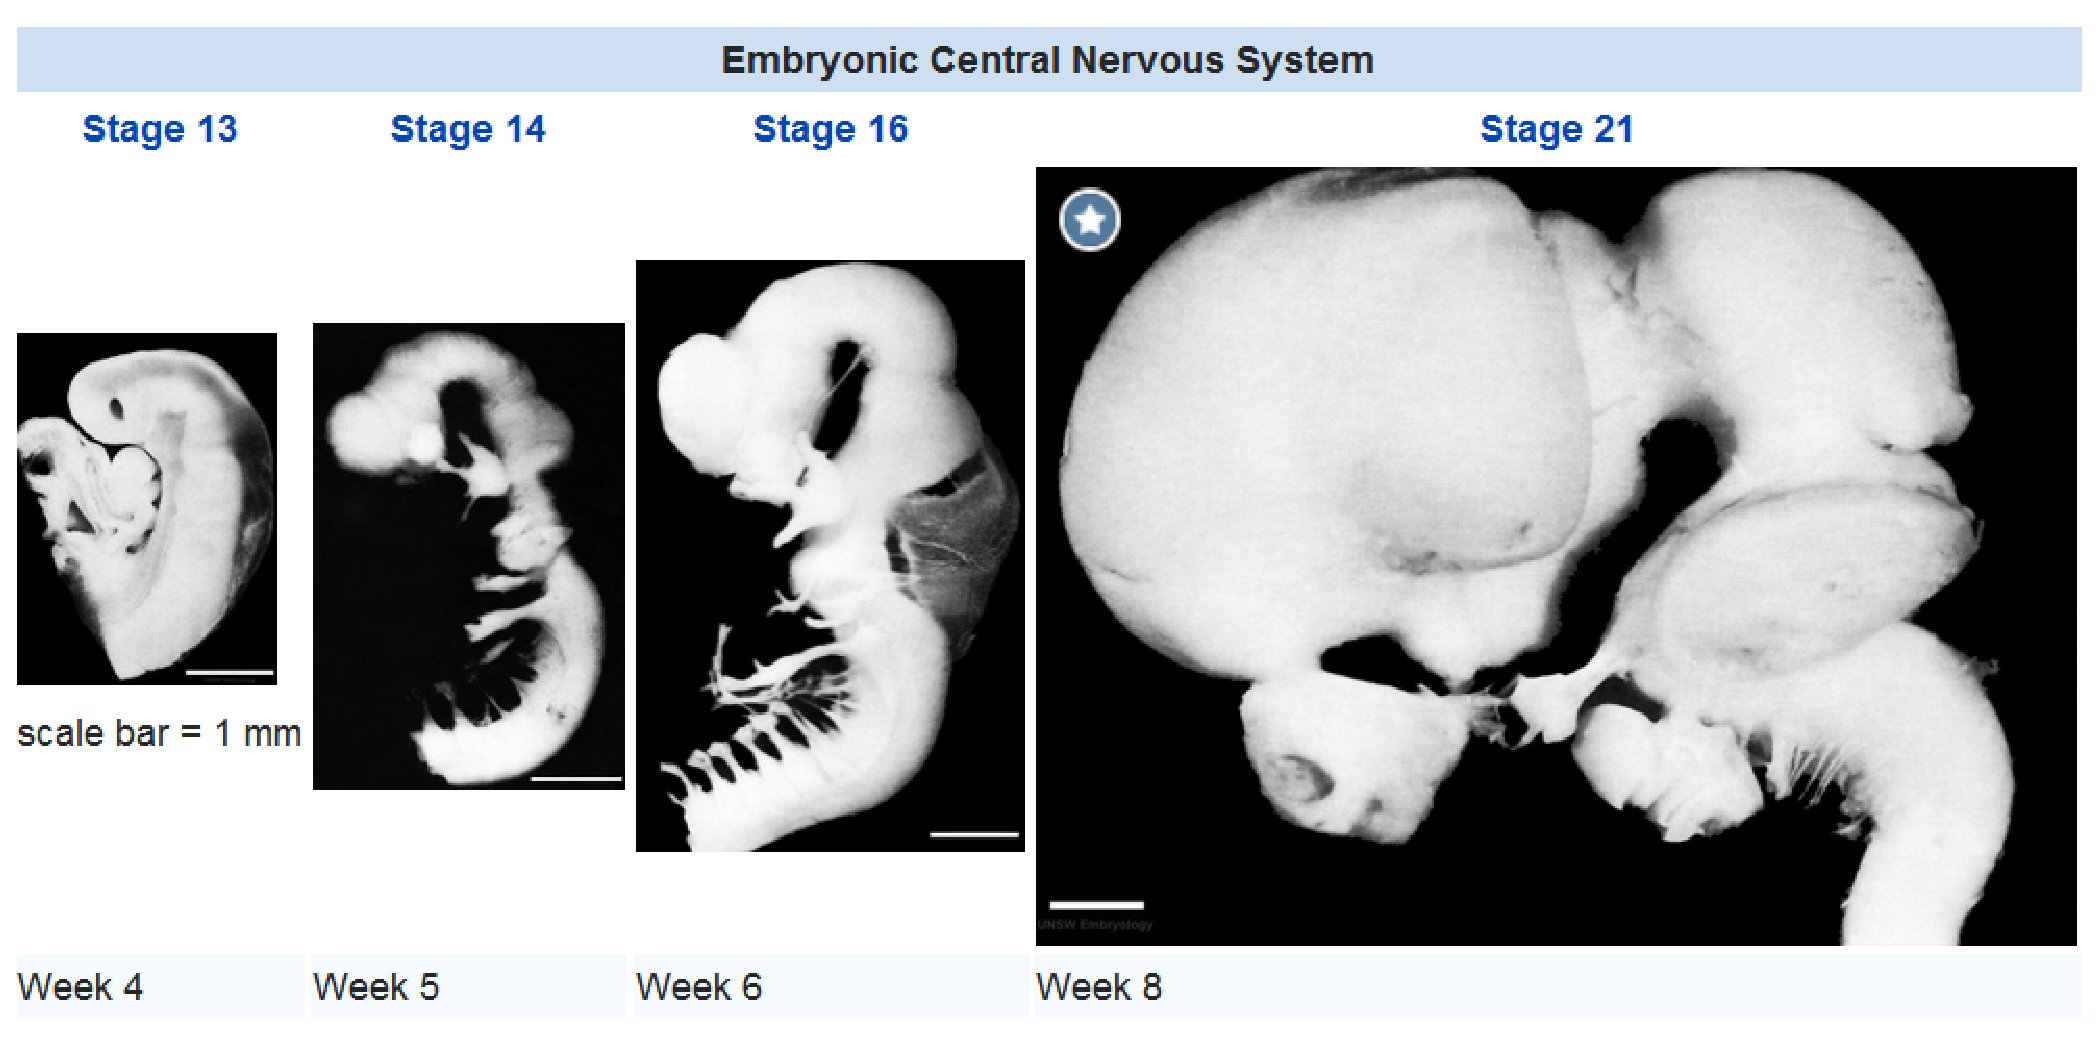
\includegraphics[height=4cm,
    angle=0]{./images/embryonic-CNS.eps}}
\caption{Embryonic CNS
\footnote{\url{https://embryology.med.unsw.edu.au/embryology/index.php/Neural_System_Development}}}
\label{fig:embryonic-CNS}
\end{figure}

\subsection{-- week 3}
\label{sec:endoderm}
\label{sec:mesoderm}
\label{sec:ectoderm}

At week 3, there are 3 key processes. 
\begin{enumerate}
  \item  First is {\bf gastrulation} - the forming
of a structured called {\bf gastrula} with three distinguisable regions   
\begin{itemize}
  \item endoderm (internal layer): face the uterine cavity
  \item mesoderm : 
  \item ectoderm (external layer): closest to the uterine wall
\end{itemize}
Each region contains specific cells that will eventually differentiate into the
different organs and body parts. \textcolor{blue}{The nervous system is
developed from {\bf ectoderm}}; while cardiac muscle is developed from mesoderm.
\url{http://www.biophylaxis.gr/images/en/cell_differentiation.jpg}

  \item 
  Second is somitogenesis, 
  
  \item 
  Third is {\bf neuralation}. In neuralation,
  at day 17-19 (Carnergie stage 8), the embryo reaches an elongated and flattended state
and the {\bf neural plate} is formed. At day 20-21, two neural folds at the
borders of the neural plate appears and fuse together making the {\bf neural
tube} -
\textcolor{red}{the embryonic disk in tubular shape from which the brain and
spinal cord are developed}.
\footnote{\url{http://www.nchpeg.org/nutrition/images/stories/mthfr/neural_tube.JPG}}

\end{enumerate}

\begin{figure}[hbt]
  \centerline{
  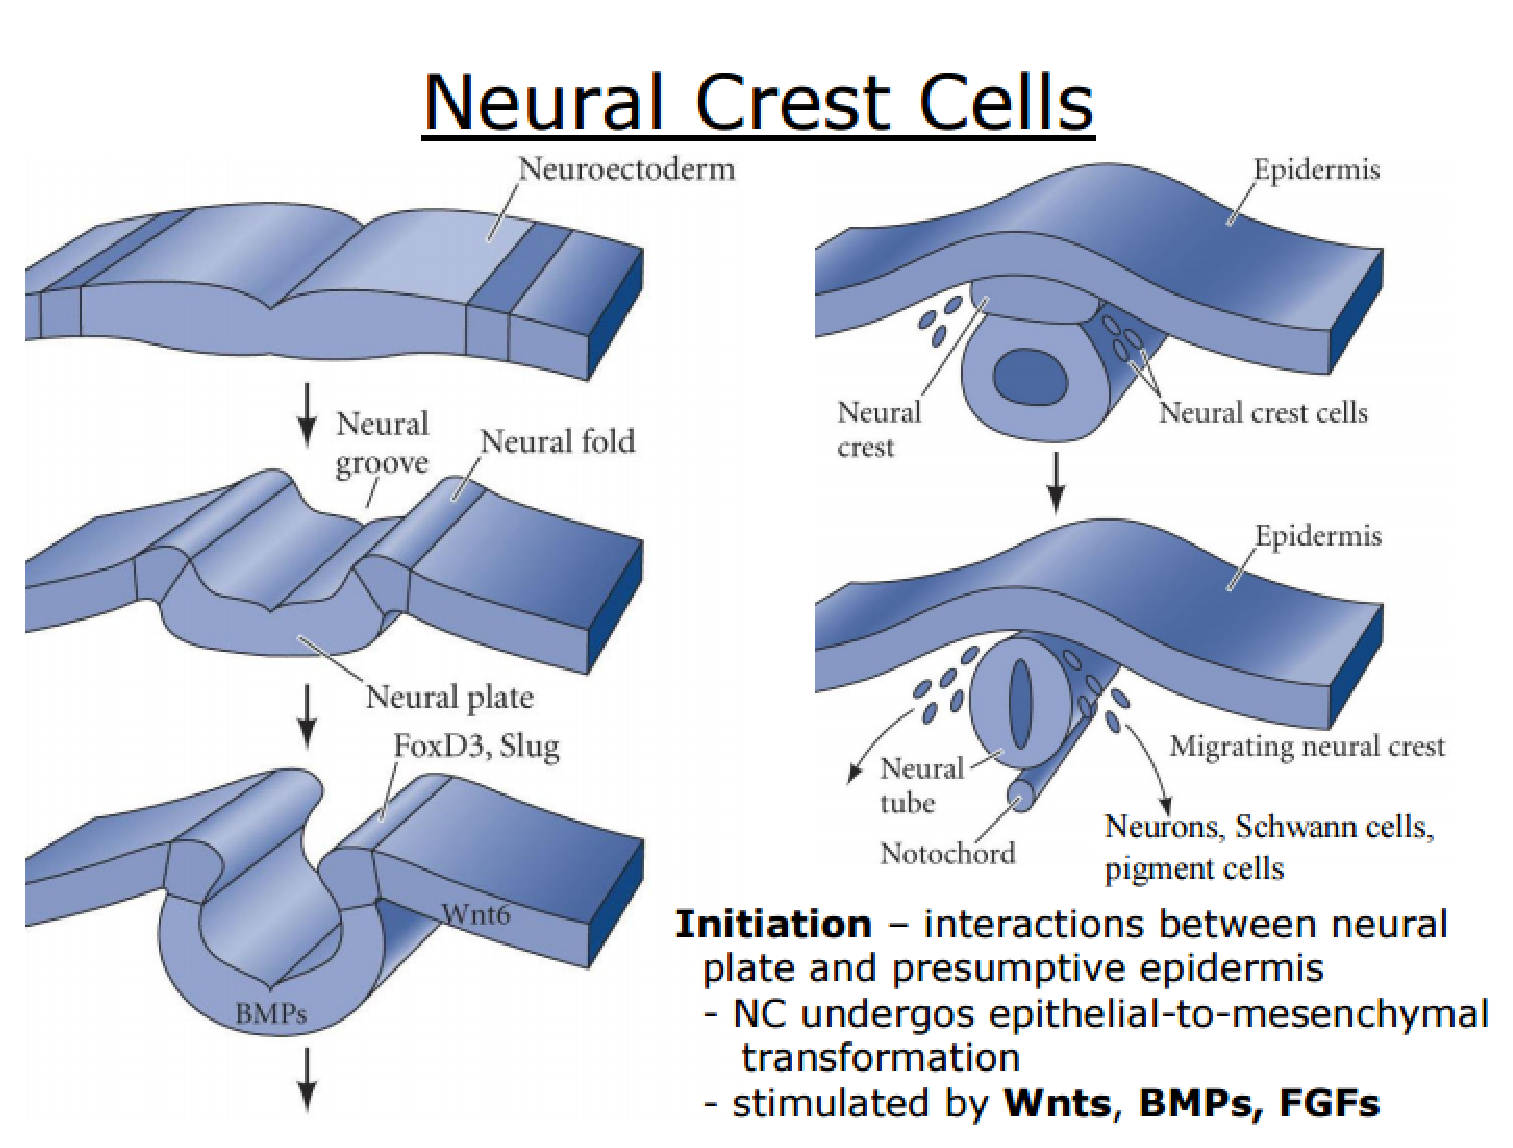
\includegraphics[height=7cm,
    angle=0]{./images/neural_crest_cells.eps}
  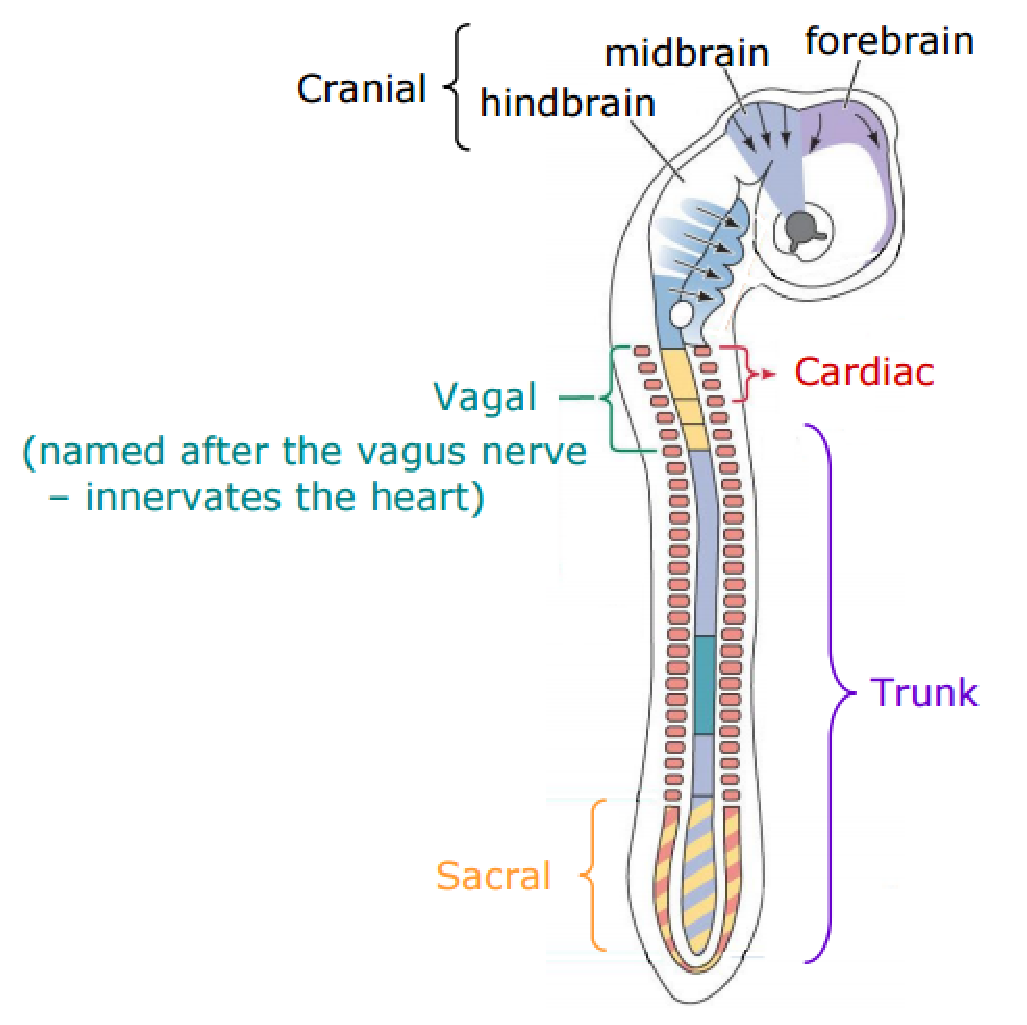
\includegraphics[height=4cm,
    angle=0]{./images/crest_cell_regions.eps}  }
\caption{Epidermis, Neural tube, and Neural crest cells. These genes are neural
crest specifiers (as they are activated during this):
Slug/Snail, FoxD3, Sox10, Sox9, AP-2 and c-Myc
\footnote{\url{http://www.d.umn.edu/~pschoff/documents/NeuralCrest_000.pdf}}}
\label{fig:neural_crest_cells}
\end{figure}

{\bf Neural crest} (4th germ layer): The cells in the neural plate not involving
in forming the neural tube form two longitudinal structures on the dorsal side of the neural
tube, called {\bf neural crest} which looks like the roof plate of the neural
tube, Fig.\ref{fig:neural_crest_cells}.
Neural crest is called the 4th germ layer as the cells in neural crest migrates
extensively to form different neural and non-neural cell types at different
regions, e.g. cranial neural crest, cardiac neural crest, trunk neural crest,
vagal and sacral neural crest.
\url{http://www.ncbi.nlm.nih.gov/books/NBK10065/}
\url{https://embryology.med.unsw.edu.au/embryology/index.php/Neural_Crest_Development}



\begin{figure}[hbt]
  \centerline{
  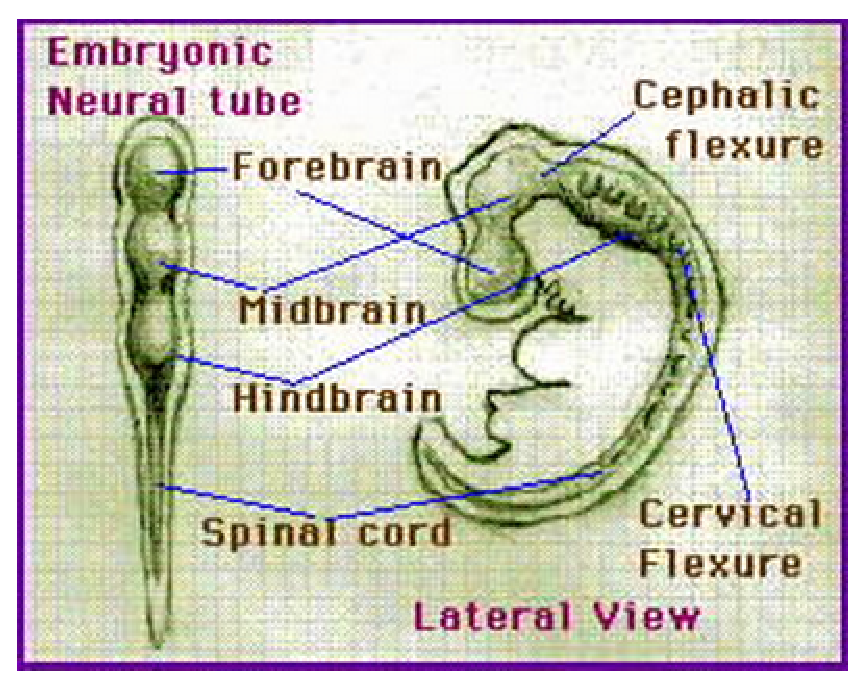
\includegraphics[height=5cm,
    angle=0]{./images/neural_tube.eps}}
\caption{Neural tube with three distinct cavities: forebrain, midbrain, and
hindbrain}
\label{fig:neural_tube}
\end{figure}
 
\subsection{-- week 4}

{\bf At 3-4 weeks}, the neural tube is divided into four unseparated regions
which are then developed into three distinct, but connected rounded cavities
(vesicles) and the fourth one is the spinal cord, Fig.\ref{fig:neural_tube}. 
This stage is called {\it three-vesicle stage}.
At this stage of development the embryo is curled and it is possible to notice
where the head is located.

\begin{mdframed}

Later on: the three vesicles (prosencephalon, mesencephalon, and
rhombencephalon) maps to forebrain (Sect.\ref{sec:forebrain}), midbrain
(Sect.\ref{sec:midbrain}) and hindbrain (Sect.\ref{sec:hindbrain}).

Also, the top and the bottom vesicle, each splitting while the middle one
staying as it, i.e. finally forming 5 vesicles. In particular, the forebrain
splits into telencephalon and diencephalon. The hindbrain splits into myelencephalon
(medulla) and metencephalon (pons \& cerebellum).
\end{mdframed}

\subsection{-- week 6}

{\bf At week 6}: the neural tube 'zips up' along its length to close and protect
the brain and spinal cord, Fig.\ref{fig:neural_crest_cells}. If the neural tube
doesn't close at any part along its length, the baby will  have a neural tube
defect (i.e. neural tube diseases - NTD) such as spina bifida, anencephaly,
encephalocele.


% In development, the forebrain develops from the {\bf prosencephalon} (i.e.
% forebrain), the most anterior vesicle of the neural tube that later forms both
% the diencephalon and the telencephalon. The {\bf Telencephalon} (the cerebral
% hemispheres) is the largest of the divisions of the human brain, and {\bf
% diencephalon} (interbrain) is the region of embryonic vertebrate neural tube
% that gives rise to posterior forebrain structures. In adults, the diencephalon
% appears at the upper end of the brain stem, situated between the cerebrum and
% the brain stem (Sect.\ref{sec:diencephalon}).

\url{http://www.us.elsevierhealth.com/media/us/samplechapters/9780443104077/Chapter 02.PDF}

\subsection{-- week 8}

Gestational week eight (GW8) is the time in human embryonic period in that
there is rapid growth and elaboration of both cortical and subcortical
structures, including the rudiments of the major fiber pathways.

Neuron production in humans begins on embryonic day 42. E42, i.e. 42 days post
conception (Bystron et al. 2008; Stiles 2008) and is largely complete by
midgestation.

By the end of the prenatal period major fiber pathways, including the
thalamocortical pathway, are complete. 

\subsection{* forebrain (prosencephalon): telencephalon and diencephalon}
\label{sec:forebrain}

{\bf Prosencephalon} ({\it forebrain} - most anterior cavity (vesicle)) is the
pre-embryonic structure which then develops further into {\it diencephalon}, and
{\it telencephalon}, Fig.\ref{fig:prosencephalon}.

\begin{figure}[hbt]
  \centerline{
  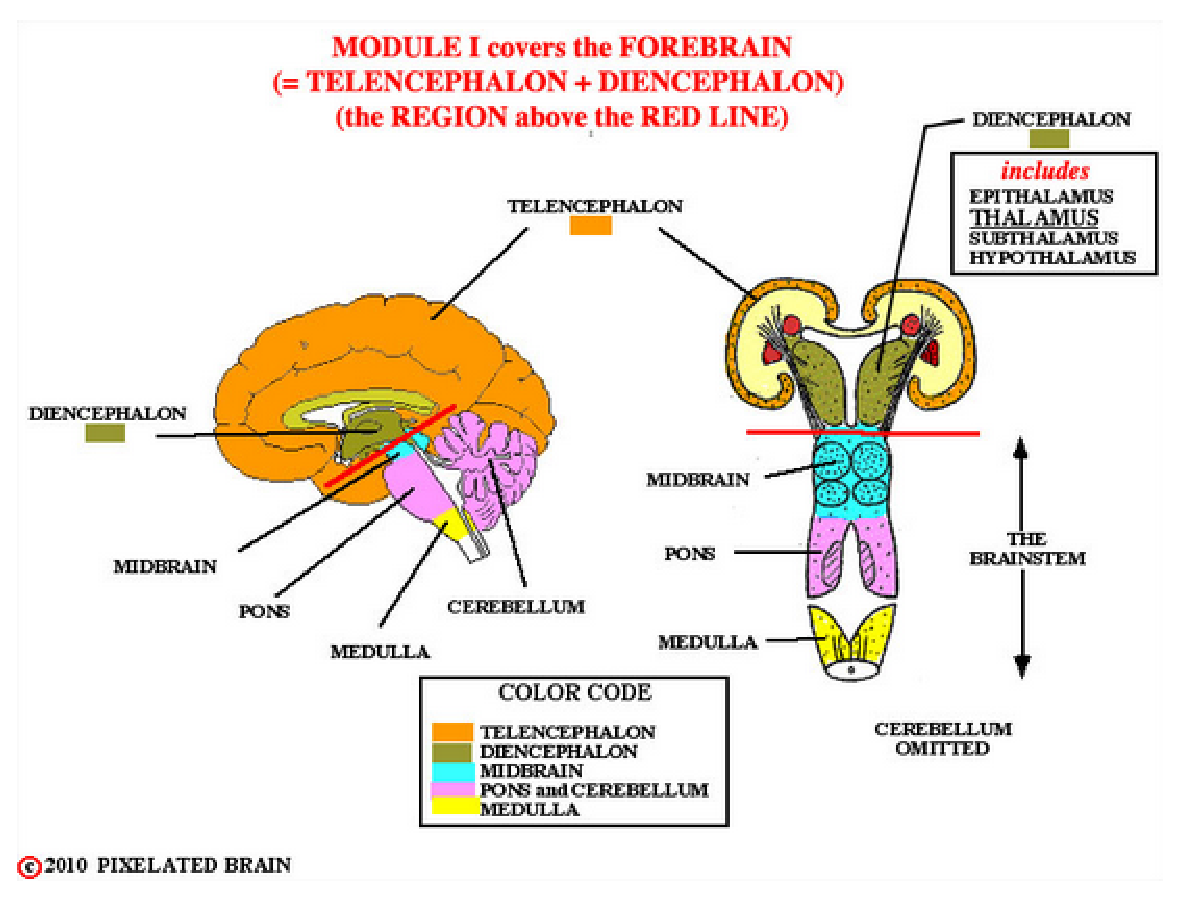
\includegraphics[height=7cm,
    angle=0]{./images/prosencephalon.eps}}
\caption{Telencephalon, Diencephalon (epithalamus, thalamus, subthalamus,
hypothalamus), Mesencephalon (Midbrain), Myelencephalon (Medulla),
Metencephalon(Pons, Cerebellum)}
\label{fig:prosencephalon}
\label{fig:mesencephalon}
\label{fig:myelencephalon}
\end{figure}

The anterior part of the brain (forebrain) in vertebrates, fish, amphibia, and
reptiles is relatively underveloped. In these animals, the forebrain appears to
be related to the olfactory system (thus term {\it rhinencephalon}
(smell-brain) - Sect.\ref{sec:olfactory-bulb}).

The forebrain in the mammals developed to the extent making it comprising most
of the mass of the CNS. The part of the forebrain in the mammals that seems to
be homologous to the forebrain in the lower vertebrates retain the name
rhinencephalon (and also called {\it archipallium}). However, the rhinencephalon
in mammals, with evolution, has also acquired many additional connections with
other parts of the forebrain. The part of the forebrain that has developed
mostly in mammals is called {\it neopallium} (or neocortex) -
Sect.\ref{sec:neocortex}.



\subsection{-- telencephalon}
\label{sec:telencephalon}

{\bf Telencephalon} is the embryonic structure in forebrain
(Sect.\ref{sec:forebrain}) which develops into cerebrum (the outer most and
upper most part of the brain) - Sect.\ref{sec:cerebrum} - which is the largest
of the divisions of the human brain. The word {\bf cerebrum} comes from Latin,
where it means "brain".  In English it refers to the major part of the brain.

In mammals, we have more details
\begin{itemize}
  \item dorsal telencephalon (i.e. pallium): develops into cerebral cortex
  
  \item ventral telencephalon (i.e. subpallium): develops into basal ganglia
\end{itemize}


\subsection{--  diencephalon (interbrain)}
\label{sec:diencephalon}  

{\bf Diencephalon} (interbrain, diencephalic structure) is the embryonic
structure in forebrain (Sect.\ref{sec:forebrain}), and develops into 4 distinct
posterior forebrain structures of thalamus (from Greek means {\it chamber}).
\begin{enumerate}
  \item {\it dorsal thalamus} (or simply thalamus -
Sect.\ref{sec:thalamus}), 

  \item {\it subthalamus} (Sect.\ref{sec:subthalamus}), 
  
  \item {\it hypothalamus} - Sect.\ref{sec:hypothalamus}, 

  \item and {\it epithalamus} (Sect.\ref{sec:epithalamus}).
\url{http://en.wikipedia.org/wiki/Diencephalon}
\end{enumerate}


In adult mammals, the diencephalon appears at the upper end of the brain stem,
situated between the cerebrum and the brain stem. The function is discussed in
Sect.\ref{sec:thalamus-function}.

  

\subsection{* midbrain (mesencephalon)}

{\bf mesencephalon} ({\it midbrain} - second cavity)
  
(no change)

\subsection{*hindbrain (rhombencephalon): myelencephalon + metencephalon}
\label{sec:hindbrain}

During embryonic stages, the hindbrain is developed from the {\bf
rhombencephalon} vesicle ({\it hindbrain} - the caudal cavity). 

It develops further into {\it myelencephalon} and
{\it metencephalon}.

\begin{enumerate}
  \item myelencephalon - Sect.\ref{sec:myelencephalon}
  \begin{itemize}
    \item  medulla oblongata (Sect.\ref{sec:medulla_oblongata}) 
  \end{itemize}

  \item metencephalon - Sect.\ref{sec:metencephalon}
  \begin{itemize}
    \item pons - Sect.\ref{sec:pons}
    \item cerebellum - Sect.\ref{sec:cerebellum}
  \end{itemize}
\end{enumerate}

\subsection{--  myelencephalon: medulla oblongata, reticular formation}
\label{sec:myelencephalon}

{\bf Myelencephalon} is the posterior portion of the brain stem, which as
described below, is composed largely of tracts carrying signals between the rest
of the brain and the body. The caudal end of the myelencephalon develops into
the spinal cord  (Sect.\ref{sec:spinal_cord}).

Myelencephalon develops into 
\begin{itemize}

  \item   medulla oblongata (Sect.\ref{sec:medulla_oblongata}) at the brainstem
  (and serves as the connection between spinal cord and the brain, Fig.\ref{fig:myelencephalon},
i.e. regulates vasomotor function and autonomic responses such as respiration
and cardiovascular systems as well as basic reflexive activities (coughing,
sneezing, swallowing, vomiting))
  
  \item reticular formation - Sect.\ref{sec:reticular-formation} - an
  interesting part from the psychological perspective.
\end{itemize}

 
 
\subsection{--  metecephalon: pons + cerebellum}
\label{sec:metencephalon}

As part of the hindbrain (Sect.\ref{sec:hindbrain}), the {\bf  metencephalon} is
composed of two main structures: the pons (Sect.\ref{sec:brain-stem}) and
cerebellum (Sect.\ref{sec:cerebellum}).

\subsection{B. Brain childhood/adolescence development}
\label{sec:brain-children}

A better understanding of normal neurodevelopment could help elucidate the
pathogenesis of disorders such as schizophrenia (Sect.\ref{sec:schizophrenia}),
in which aberrant during brain development is thought to occur before the onset
of psychotic symptoma-tology.
\citep{sowell2002}.

There are two important factors \citep{stiles2010}.  
\begin{enumerate}
  \item  gene expression: what genes are and how they play an important role in
  brain development
  
  \item the outcome of brain development, the mature brain: what are the major
  structures and what are the basic principles of brain organization
\end{enumerate}

\subsection{-- size}

The infant brain will increase in size by a factor of up to 5 by adulthood.
However, the brain increases in size by four-fold during the preschool period,
reaching approximately 90\% of adult volume by age 6. 
\begin{itemize}
  \item  Whole-brain voxel-based morphometry (VBM) to assess regional patterns of gray-
and white-matter maturation and similar results have been observed with most
prominent at the age between 7-16 years of age.
  \item The volumetric MRI studies on postmortem have given that cortical gray-matter
volume reductions appear to be somewhat specific to the superior cortices of the
frontal and parietal lobes relatively late in development (i.e. between
childhood and adolescence).

  \item Male brain volumes tend to be larger than female brain volumes (MWU, p<0.05) by
approximately 7\%. Regionally, only the frontal and parietal lobes and the
subcortical region differbetween males and female.

  \item With the exception of the thalamus, all subcortical regions were significantly
correlated with total brain volume.
\end{itemize}

\subsection{-- cell types}
\label{sec:brain-cells}

Neurons (Sect.\ref{sec:neuron-types}), neuroglia (astrocytes and
oligodendrocytes - Sect.\ref{sec:neuroglia-cell}), and ependymal cells
(Sect.\ref{sec:ependymal-cell}) are three distinct categories of neural cells in
the central nervous system (Chap.\ref{chap:cells-CNS}).

During development, the precursors for all of these cells reside within the
epithelium of the neural plate and its successor, the neural tube. The cavity
formed inside the neural tube is surrounded by the neural precursor cells the
give rise to different cell types in the neurons of the CNS
(Sect.\ref{sec:neuron-types}). This cavity will eventually form the ventricles
(Sect.\ref{sec:ventricle_brain}).

There are many different kinds of neurons that vary in their size and shape as
well as in their function (Sect.\ref{sec:neuron-type-classification}). Neurons
make connections with other neurons to form the information processing networks
that are responsible for all of our thoughts, sensations, feelings and actions.


\subsection{-- number of neurons and connectivity}

At birth, the human brain consists of approximately 86 ($\pm$ 8) billion
neurons; and reaches about 100 billion at matured. It means that the
number of neurons are not playing an important factor to the development of the
brain; but it is the connectivity between them (as we will discuss shortly).


Since each neuron can make connections with more than 1,000 other neurons, the
adult brain is estimated to have more than 60 trillion neuronal connections.
During the early postnatal period, level of connectivity throughout the
developing brain far exceeds that of adults (Innocenti and Price 2005). This
exuberant connectivity is gradually pruned back via competitive processes that
are influenced by the experience of the organism.

So, there are two major changes: the synaptic connections between neurons
(Sect.\ref{sec:synaptogenesis}), and the myelination of nerve fibers.
\begin{enumerate}
  \item  The increased myelination is related to improved conductivity between different
brain regions during maturation. The brain regions have been shown to mature in
a pattern generally proceeding from inferior to superior, and from posterior to
anterior structure.

  \item The structural changes in both the major gray and white matter
  compartments continue through childhood and adolescence, and these changes in
  structure parallel changes in functional organization that are also reflected
  in behavior.
\end{enumerate}



\subsection{C. Brain evolution}
\label{sec:brain_evolution}

According to Paul MacLean's theory, the following three distinct brains emerged
successively in the course of evolution and now co-inhabit the human skull:

\subsection{-- archipallium (primitive brain)}
\label{sec:archipallium}

{\bf archipallium} (primitive brain): controls the body's vital 
  functions such as heart rate, breathing, body temperature and balance

  
Example: reptilian brain (the oldest of the three, first appear about 500
million years ago):  include the brainstem and the cerebellum. 
  
\subsection{-- paleopallium (add limbic system)}
\label{sec:paleopallium}

{\bf paleopallium}:  adding the limbic system (Sect.\ref{sec:limbic-system},
first appear about 150 million years ago):  emerged first in the mammals; with
the main structures of the limbic brain are the hippocampus, the amygdala, and
the hypothalamus.
  
The limbic brain is the seat of the value judgments that we make, often
unconsciously, that exert such a strong influence on our behaviour.

\subsection{-- neopallium}
\label{sec:neopallium}
  
{\bf neopallium} - neocortex brain (first appear about 2-3 million years
  ago):   the two hemispheres of the neocortex have been responsible for the
  development of human language, abstract thought, imagination, and consciousness.
  The neocortex is flexible and has almost infinite learning abilities.
  
  As the cortex grows much faster than the skull, it acquired many folds. The
  very deep folds of the cortex are called fissures, and the shallower folds are
  called sulci (Sect.\ref{sec:sulcus}).

\url{http://thebrain.mcgill.ca/flash/d/d_05/d_05_cr/d_05_cr_her/d_05_cr_her.html}


\subsection{D. Brain's anatomy}
\label{sec:brain-anatomy}
\label{sec:coronal-plane}
\label{sec:hirozontal-plane}
\label{sec:sagittal-plane}

The brain is the most complex part of the body (Sect.\ref{sec:encephalon}). The
brain is divided into many parts that serve specific and of course important
functions.

To understand the brain's anatomy, the brain is often cut into series of
sections, in one of three different traditional directions,
Fig.\ref{fig:brain-cut}: coronal, horizontal and saggital planes. Then, the
neuron is stained using a proper technique (Sect.\ref{sec:stain-neuron}).
A very nice video that show the anatomy of the brain can be obtained
from \href{http://www.youtube.com/watch?v=HVGlfcP3ATI}{YouTube}.

\begin{figure}[hbt]
  \centerline{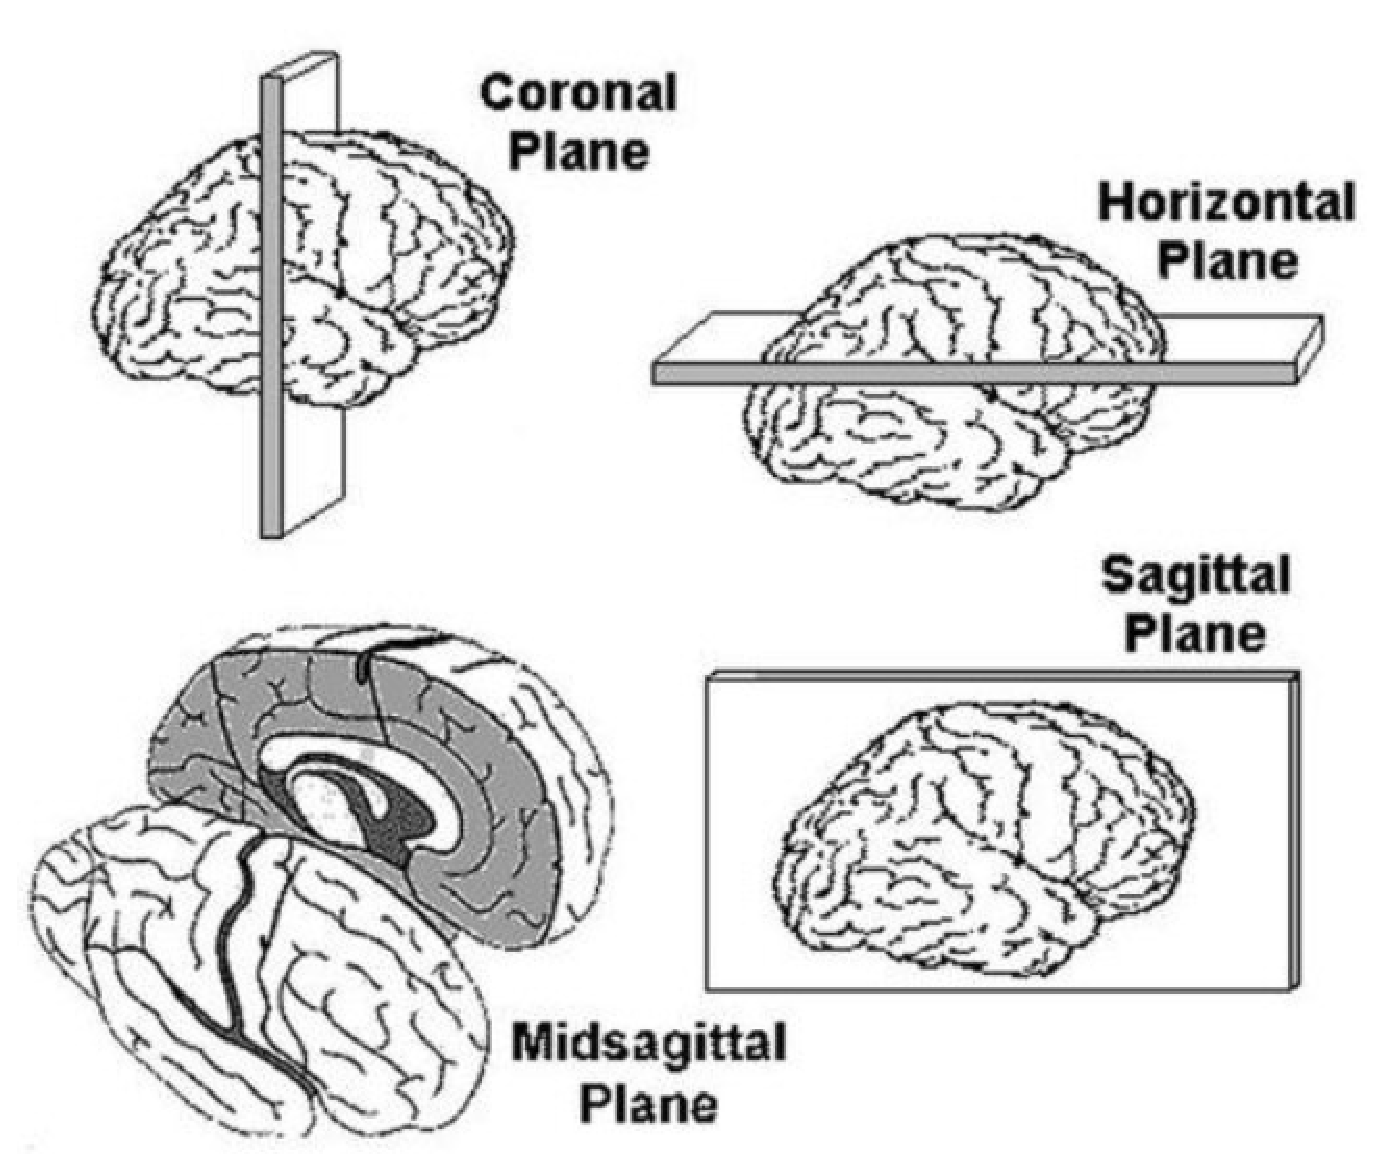
\includegraphics[height=5cm,
    angle=0]{./images/brain-cut.eps}}
  \caption{Brain's cut: coronal plane, horizontal plane, and sagittal plane
  (e.g. midsagittal plane)}
\label{fig:brain-cut}
\end{figure}

The brain is developed during embryonic period from 5 vesicles (see above)
expanding to make up this brain. There are different ways to define the anatomy
of the brain
\begin{enumerate}
  \item 3 major parts: - Sect.\ref{sec:anatomy-3parts} 
  
  \item based on the colors (2 types) - Sect.\ref{sec:anatomy-colors}

  \item (only for cortex) Broadmann areas - Sect.\ref{sec:Brodmann_area}

\end{enumerate}

The largest and most important brain information processing networks involve the
{\bf neocortex} and the many {\bf subcortical nuclei} that relay information to
and from the neocortex.

\subsection{* cerebrum + cerebellum + brain stem}
\label{sec:anatomy-3parts}

If we look at the outside, as shown in Fig.~\ref{fig:brain_structure}, it
is visible three main parts
\begin{enumerate}
  \item cerebrum - Sect.\ref{sec:cerebrum}
  \item cerebellum - Sect.\ref{sec:cerebellum}
  \item (a portion of the) brain stem - Sect.\ref{sec:brain-stem}
\end{enumerate}

\begin{figure}[hbt]
  \centerline{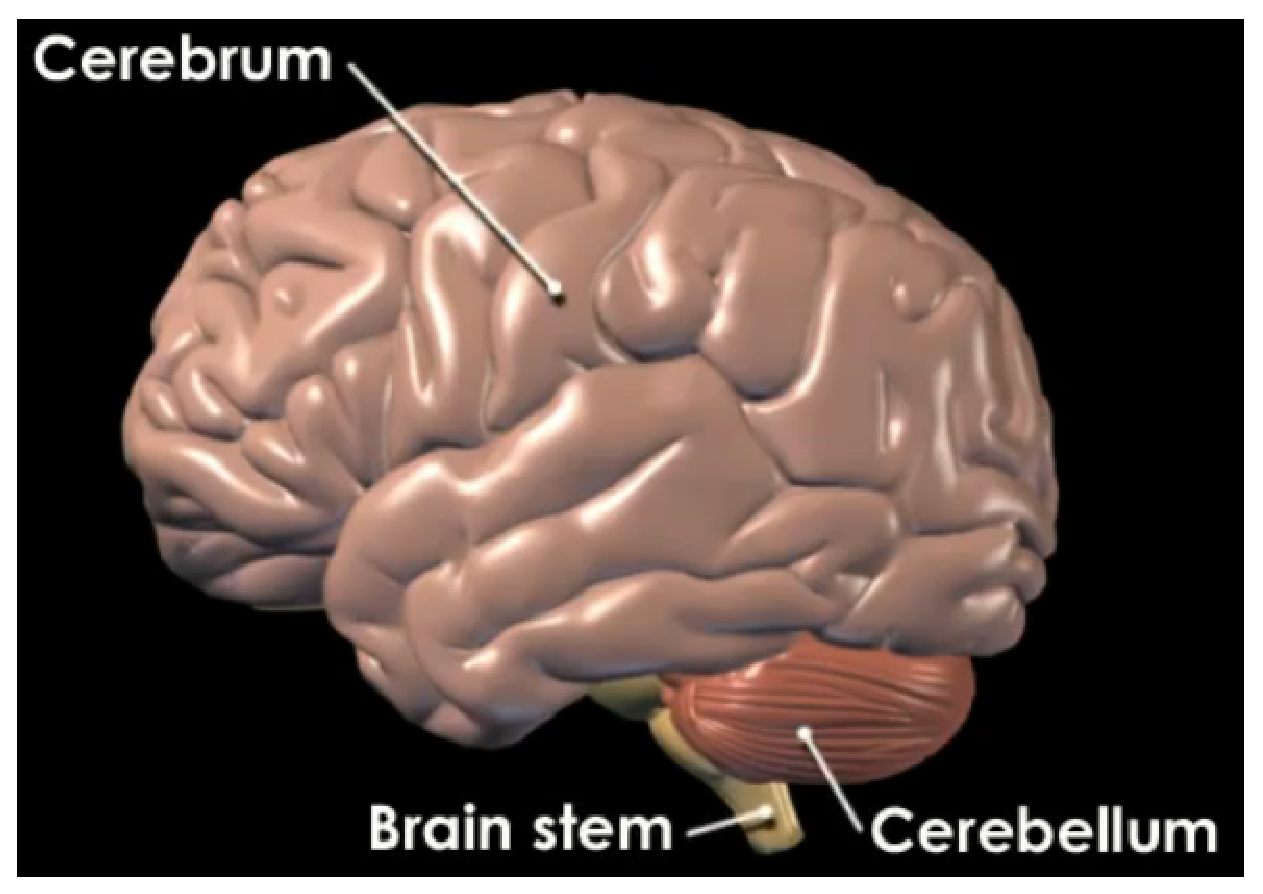
\includegraphics[height=4cm,
    angle=0]{./images/brain_01.eps}}
\caption{Brief view of the brain (from left side)}
\label{fig:brain_structure}
\end{figure}

\subsection{* grey matter + white matter}
\label{sec:anatomy-colors}

A coronal section of the cerebrum and cerebellum shows two parts
with different colors:  grey matter, white matter.
\begin{itemize}

  \item {\it grey matter}: This is where all the nerve cell body (soma),
  including the dendrites, and axon terminal reside.
  
  In the cerebrum, grey matter is a thin layer appeared actually as pinkish-grey
  color (the pinkish due to blood capillaries).
  
%   (outermost for the case of cerebrum and cerebellum; and innermost for the
%   case of spinal cord)
 
  \item {\it white matter}:  white matter is made of axons - the region where the
  myelinated-sheath neuron process - connecting various grey matter areas.
  
  In the cerebrum, white matter presents as a thicker layer than grey matter.
  
\end{itemize}

The presence of white and grey matter is reversed in the brain (the cerebrum
(Sect.\ref{sec:cerebellum}), cerebellum, brain stem), and throughout the spinal
cord (Sect.\ref{sec:spinal_cord}).
 
\textcolor{red}{Cerebral- and spinal white matter do not contain dendrites,
neural cell bodies, or shorter axons}. These are found only in grey matters.
IMPORTANT: 
\begin{itemize}
  \item  The spinal cord has grey matter on the inside and white matter on the
outside.

  \item The Brain has grey matter on the outside and white matter on the inside.

\end{itemize}
% The grey matter locates on the most peripheral edges of the cerebrum, with the
% white matter underneath.
\url{http://web.stanford.edu/group/hopes/cgi-bin/hopes_test/the-hopes-brain-tutorial-text-version/}


%\url{http://web.stanford.edu/group/hopes/cgi-bin/hopes_test/the-hopes-brain-tutorial-text-version/}

% {\bf Cerebrum} (Sect.\ref{sec:cerebrum}) is the most anterior part and most
% superior region in the vertebrate CNS. It grows out of the metencephalon
% (Sect.\ref{sec:metencephalon}). It is divided into symmetric left and right
% hemisphere, known as {\it cerebral hemisphere}.
% The hemispheres communicate with each other through a thick band of 200-250
% million nerve fibers called the {\bf corpus callosum}
% (Sect.\ref{sec:corpus_callosum}). If we divide the cerebrum further, it is
% divided into different {\bf lobes} (Sect.\ref{sec:lobes})
% \begin{enumerate}
%   \item frontal lobe
%   \item parietal lobe
%   \item occipital lobe
%   \item temporal lobe
% \end{enumerate}
% The border between the lobes are anatomically marked by the different {\bf
% sulci}. 




References:
\begin{enumerate}
\item \url{http://www.brainviews.com/abFiles/DrwMedlobes.htm}
\item \url{http://faculty.stcc.edu/AandP/AP/AP1pages/nervssys/unit13/cerebrum.htm}
\end{enumerate}

\subsection{* Brodmann areas (in cortical regions)}
\label{sec:area_in_brain}
\label{sec:Brodmann_area}

Korbinian Brodmann, based on Nissl staining method, published a map of cortical
areas into different regions in 1909, for humans, monkeys, and other species.
A similar, but more detailed cortical map was published by Constantin von
Economo and Georg N. Koskinas in 1925.

IMPORTANT: The same Brodmann area number in different species does not
necessarily indicate homologous areas.

IMPORTANT: The map has been refined so many times.
\textcolor{red}{The same Brodmann area number in different species does not
necessarily indicate homologous areas}.

\begin{figure}[hbt]
  \centerline{
  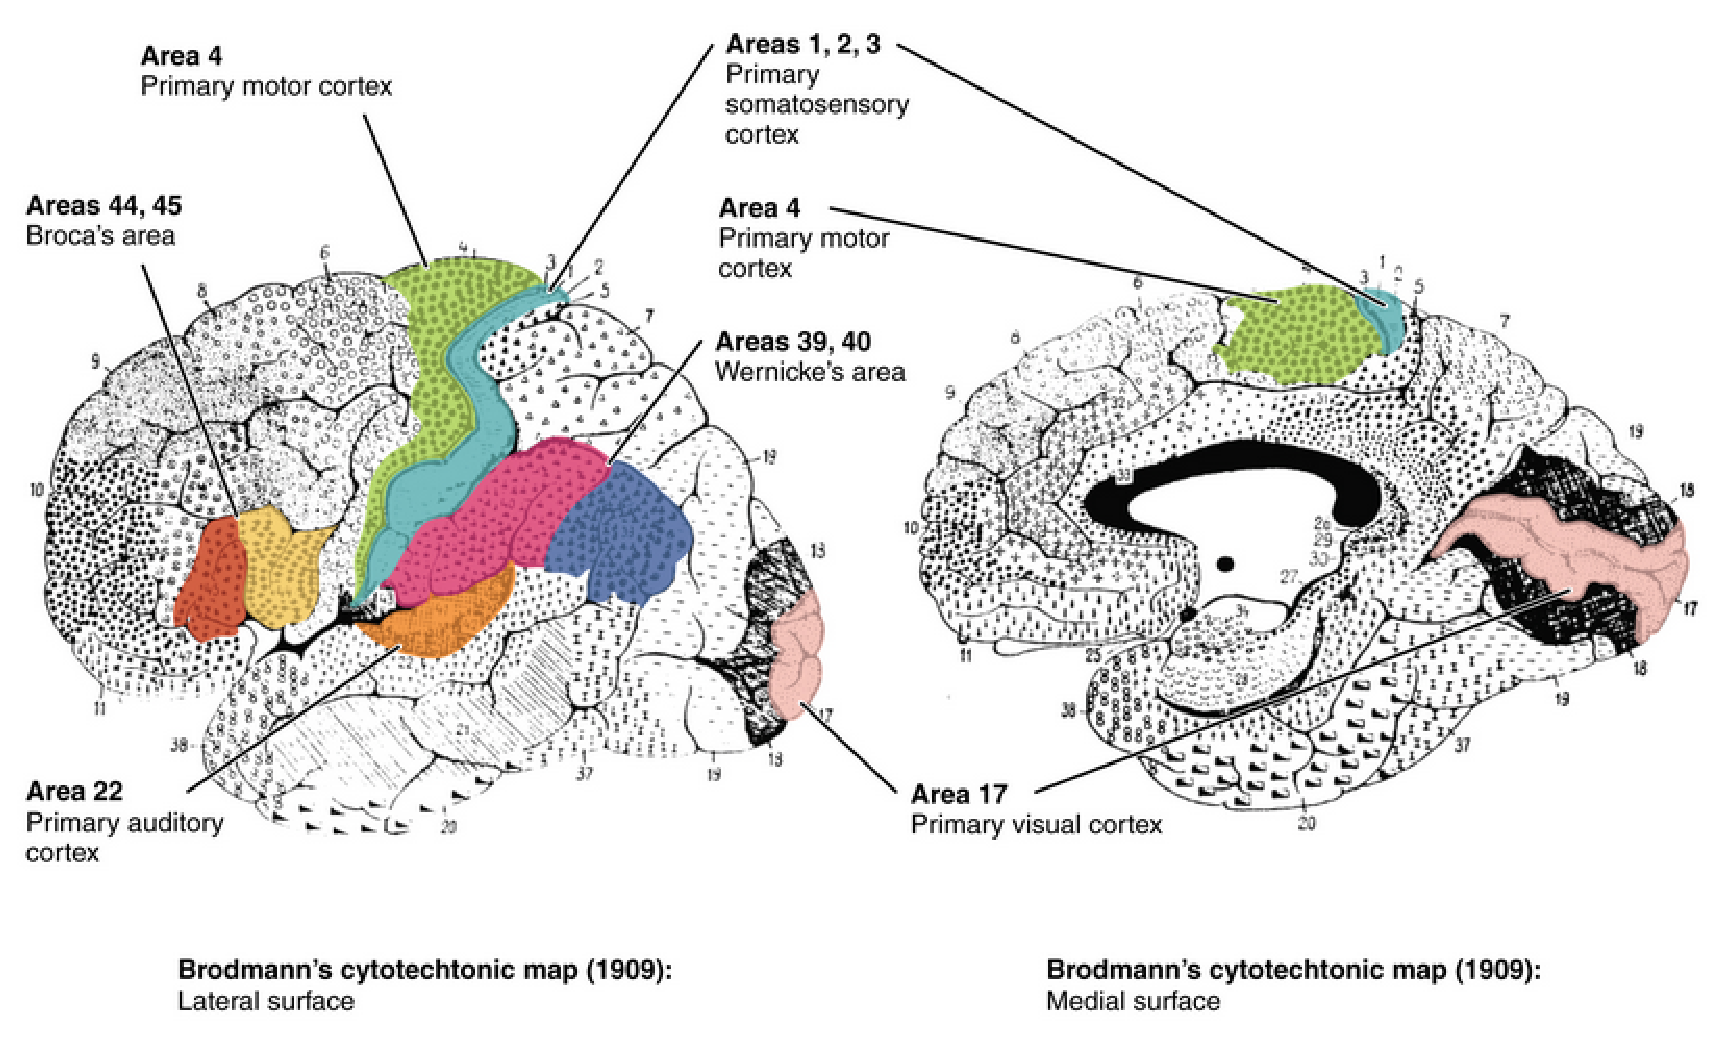
\includegraphics[height=7cm,
    angle=0]{./images/brain_areas.eps}}
\caption{Brodmann area}
\label{fig:brain_areas}
\label{fig:Brodmann_area}
\end{figure}

In humans and other primates:
\begin{itemize}
  \item area 1, 2, 3:  primary somatosensory cortex (Sect.\ref{sec:somatosensory-cortex})
  \item area 4: 	 primary motor cortex (Sect.\ref{sec:motor-cortex})
  \item area 6: premotor cortex
  \item area 5, 7: Somatosensory Association Cortex
  \item area 8: Includes Frontal eye fields
  \item area 9: granular frontal cortex
  \item area 10: frontopolar prefrontal cortex
  \item area 17: primary visual cortex
  
  \item area 25: subgenual cortical areas -
  Sect.\ref{sec:subgenual-cortical-area}
  
  \item area 39, 40: Wernicke's area
  \item area 41, 42: primary auditory cortex (and partially area 22)
  \item area 44, 45: Broca's area
  \item area 46: dorsolateral prefrontal cortex (dLPFC) 
  
\end{itemize}
\url{http://en.wikipedia.org/wiki/Brodmann_area}





\subsection{* ventricular system (cavities)}
\label{sec:ventricle_brain}

A ventricle is a cavity inside the brain. There are total 4 interconnected
cavities (ventricles) in the brain where the cerebrospinal fluid (CSF) is
produced - Sect.\ref{sec:CSF}, Fig.\ref{fig:ventricle_brain}.

The choroid plexuses in the lateral, third and fourth ventricles produce CSF.
By producing CSF, the main function of ventricular system is to protect the
human brain from trauma (via a cushioning effect created by CSF) and to help
form the central canal, which runs the length of the spinal cord.

\begin{enumerate}

  \item left and right lateral ventricles: largest

  \item third ventricle: in the diencephalon of the forebrain between the right
  and left thalamus
  
  \item fourth ventricle (developed from area inside the neural tube called the
  central cana):
  the position is within the region of mesencephalon and metecephalon, i.e.
  located at the back of the pons and upper half of the medulla oblongata of the
  hindbrain.
  
  It has a diamond shape and is located in the upper portion of the medulla.
  This ventricle has a roof and a floor. The roof is composed of the cerebellum,
   located at the back of the brain, and the floor is formed by the rhomboid
   fossa, a depression in the brainstem. 
   Within the floor is the facial colliculus, sulcus limitans, and the obex.
\end{enumerate}
\url{http://en.wikipedia.org/wiki/Ventricular_system#/media/File:Blausen_0896_Ventricles_Brain.png}

\begin{figure}[hbt]
  \centerline{ 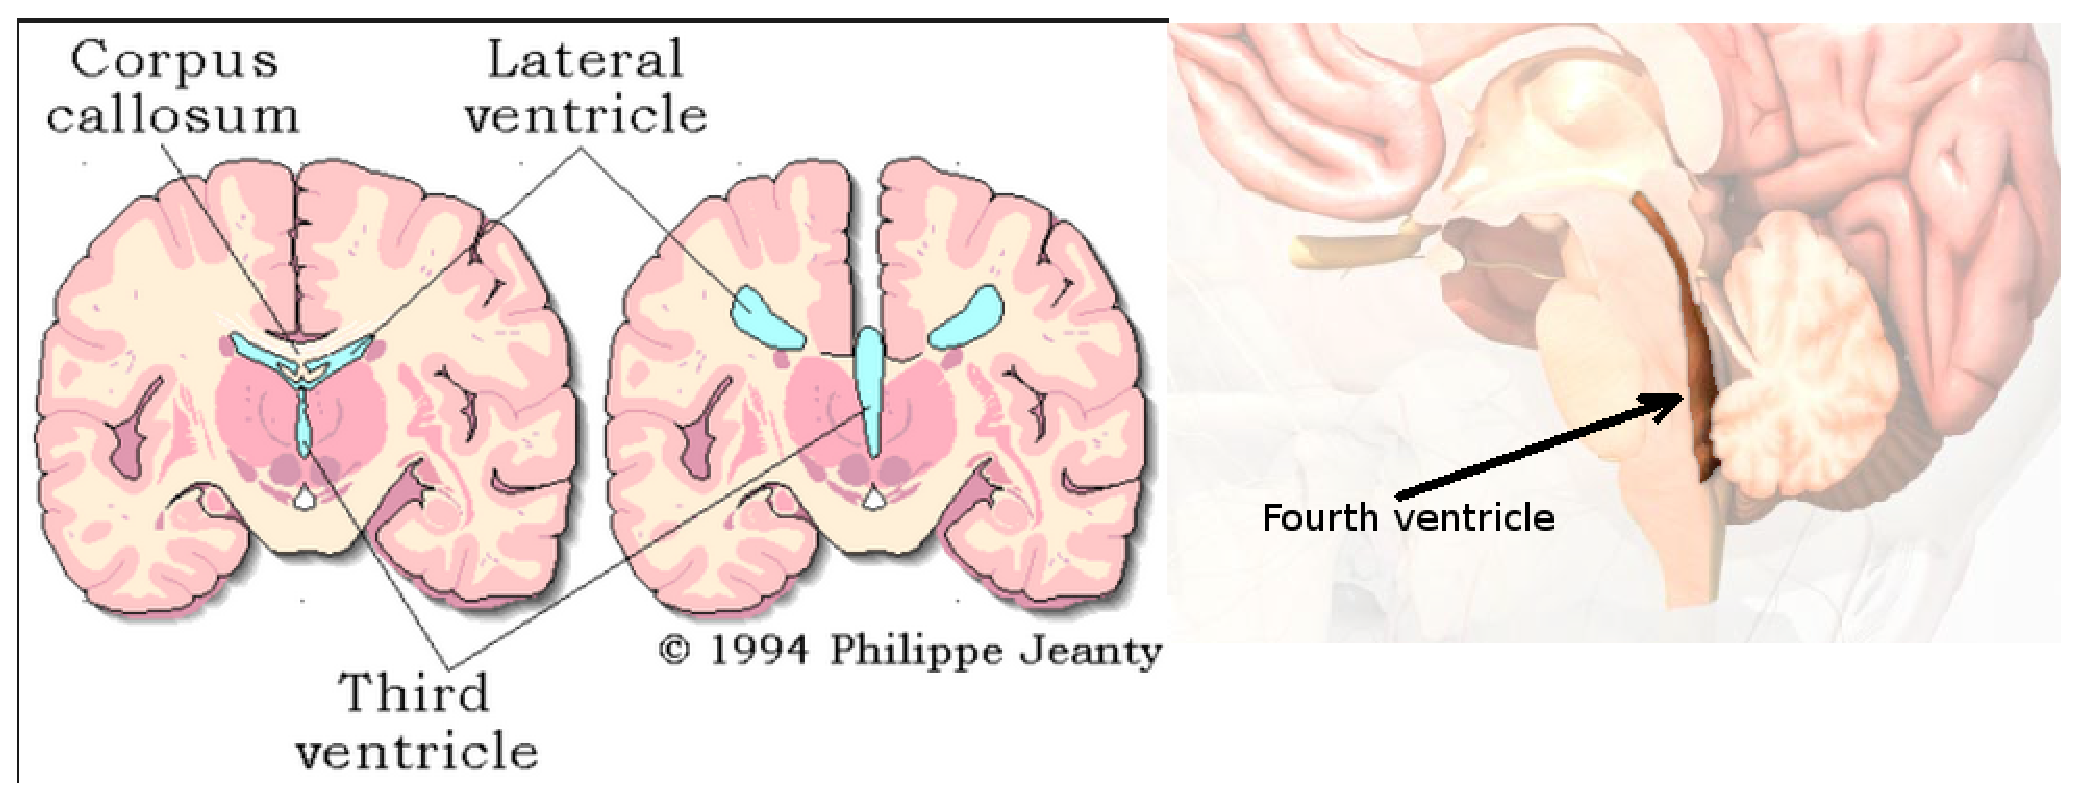
\includegraphics[height=4cm,
    angle=0]{./images/ventricle_brain.eps}}
\caption{Corpus callosum, lateral ventricles, and third ventricle: captured at
two different brain depth}
% http://www.sonoworld.com/images/FetusItemImages/article-images/central_nervous_system/dcc_images/image78.gif
%http://www.healthline.com/human-body-maps/fourth-ventricle
\label{fig:ventricle_brain}
\end{figure}

NOTE: The ventricles are formed during the first three month of pregnancy.
During this time of development, it is possible for circulation to be blocked by
overproduction of cerebrospinal fluid, causing a condition called hydrocephalus.

\subsection{* neuronal nuclei (NeuN)}
\label{sec:nuclei_structure}


There are two forms of brain structures:
\begin{itemize}
  \item brain nuclei - Sect.\ref{sec:nuclei_structure}
  
  \item layered structure - Sect.\ref{sec:layered_structure}
\end{itemize}
There are multiple types of neurons arranged in clumps (subnuclei) or layers.

The brain contains hundreds of distuinguishable nuclei, varying widely in shape
and size. {\bf Neuronal Nucleus} (pl: nuclei) is a brain structure consisting of
a small cluster of neurons - one of the most common forms of nerve cell organization (anatomically,
it's a {\it region of grey matter}, often bordered with white matter). 

\begin{mdframed}

In the peripheral nervous system, a cluster of neurons is referred to instead as
a ganglion (Sect.\ref{sec:ganglion}).

\end{mdframed}

 
Nuclei in brainstem
\begin{itemize}
  \item red nucleus
  \item vestibular nucleus, 
  \item inferior olive
\end{itemize}

Nuclei in cerebellum - Sect.\ref{sec:cerebellum}
\begin{itemize}
  \item dentate nucleus, 
  \item emboliform nucleus, 
  \item globose nucleus, 
  \item fastigial nucleus
\end{itemize}

Nuclei in basal ganglia - Sect.\ref{sec:basal-ganglia}:
\begin{itemize}
  \item striatum (caudate and putamen) - Sect.\ref{sec:striatum} 
  
  \item pallidum (globus pallidus, medial and
  lateral), 
  
  \item substantia nigra, 
  
  \item subthalamic nucleus
\end{itemize}

% Example of subcortical nuclei: 
% \begin{itemize}
%   \item basal ganglia 
%   \item cerebellum 
% \end{itemize}

\label{sec:red_nucleus}
{\it Red nucleus} (nucleus ruber) is a prominent structure in the rostral
midbrain involved in motor coordination. The name 'red' came from the fact that it has
pale pink color (which is believed due to iron that is present in at least 2
different forms: hemoglobin and ferritin).

The red nucleus receives many inputs from the cerebellum.
In humans, the majority of the output goes to the bundle of fibers continues
through the medial tegmental field toward the inferior olive of the same side,
to form part of a pathway that ultimately influence the cerebellum.

Some of the major anatomical components of the brain, such as 
\begin{itemize}
  \item thalamus
  \item hypothalamus
\end{itemize} 
are organized as clusters of interconnected nuclei. 
Each contains several dozen distinguishable substructures.


\subsection{* subcortical structure}
\label{sec:subcortical-structure}

Subcortical structures refer to a set of structures below the cortex.
There are about 20 subcortical structures (subcortical regions) in the brain,
\begin{itemize}
  \item in the forebrain - Sect.\ref{sec:forebrain}

\begin{enumerate}
  \item basal ganglia (Sect.\ref{sec:basal-ganglia})
  \item limbic system (Sect.\ref{sec:limbic-system}): amygdala, hippocampus, \ldots
  
  \item thalamus (Sect.\ref{sec:thalamus})
  \item hypothalamus (Sect.\ref{sec:hypothalamus})
\end{enumerate}

  \item in the midbrain - Sect.\ref{sec:midbrain}
  
\begin{enumerate}
  \item tectum - Sect.\ref{sec:tectum}
  
  \item tegmentum - Sect.\ref{sec:tegmentum}
\end{enumerate}

  
  \item in the hindbrain - Sect.\ref{sec:hindbrain}

\begin{enumerate}
  \item cerebellum - Sect.\ref{sec:cerebellum}
  \item reticular formation - Sect.\ref{sec:reticular-formation}
  
  \item pons - Sect.\ref{sec:pons}
  \item medulla - Sect.\ref{sec:medulla_oblongata}
\end{enumerate}  
\end{itemize}
\url{http://www.intropsych.com/ch02_human_nervous_system/subcortical_structures.html}

The subcortical structures receive massive different inputs from the cerebral
cortex (at the infragranular layer -
Sect.\ref{sec:layered_structure-functional}) and peripheral sense organs and
stretch receptors.
Through recurrent feedback loops this information is integrated and shaped to provide output which
contributes to scaling, sequencing and timing of movement, as well as learning
and automatization of motor and nonmotor behaviours.

  
\section{Cerebrum (thinking brain - cerebral cortex)}
\label{sec:cerebrum}
\label{sec:cerebral-hemisphere}
\label{sec:cerebral-cortex}

Cerebrum in Latin means 'brain'; while the English terms refers to the major
part of the brain, as we know nowadays.  {\bf Cerebrum} (cerebral hemispheres,
cerebral cortex), aka ``thinking brain'', is the most anterior and the most
superior part in the vertebrate CNS, Fig.\ref{fig:brain_structure}).

Cerebrum grows out of the metencephalon (Sect.\ref{sec:metencephalon}), and is
divided into symmetric left and right hemisphere, known as {\it cerebral
hemisphere}, communicated with each other through a thick band of nerve fibers
called the {\bf corpus callosum} (Sect.\ref{sec:corpus_callosum}).

The cerebelum contains
\begin{enumerate}
  \item two cerebral hemispheres (divided by the midsagittal plane) -
  Sect.\ref{sec:hemisphere-brain}:   
%   the outer layer of both is called {\bf
%   cerebral cortex} - Sect.\ref{sec:cerebral-cortex}.
  
%   In mammals, each hemisphere comprises the outer layer (left/right cerebral
%   cortex as grey matter), and the inner layer (white matter).

Like the cerebellum (Sect.\ref{sec:cerebellum}), in mammals, the cerebrum has
the gray matter outside, and white matter inside (Sect.\ref{sec:white-matter}),
Fig.\ref{fig:cerebrum_coronal_section}. The grey matter on cerebrum is called
{\bf cerebral cortex} (Sect.\ref{sec:cerebral_cortex}), and the white matter is
called {\bf white matter of the cerebrum}
(Sect.\ref{sec:white-matter-cerebrum}).
  
  \item several subcortical structures
  \begin{itemize}
  \item hippocampus
  \item basal ganglia
  \item olfactory bulb
  \end{itemize}
\end{enumerate}

% \begin{itemize}
%   \item {\it grey matter} (cerebral cortex): a thin layer (outermost) -
%   Sect.\ref{sec:cerebral_cortex}
%   
%   \item {\it white matter}: a thicker layer -
%   Sect.\ref{sec:white-matter}
% 
% \end{itemize}


\begin{figure}[hbt]
  \centerline{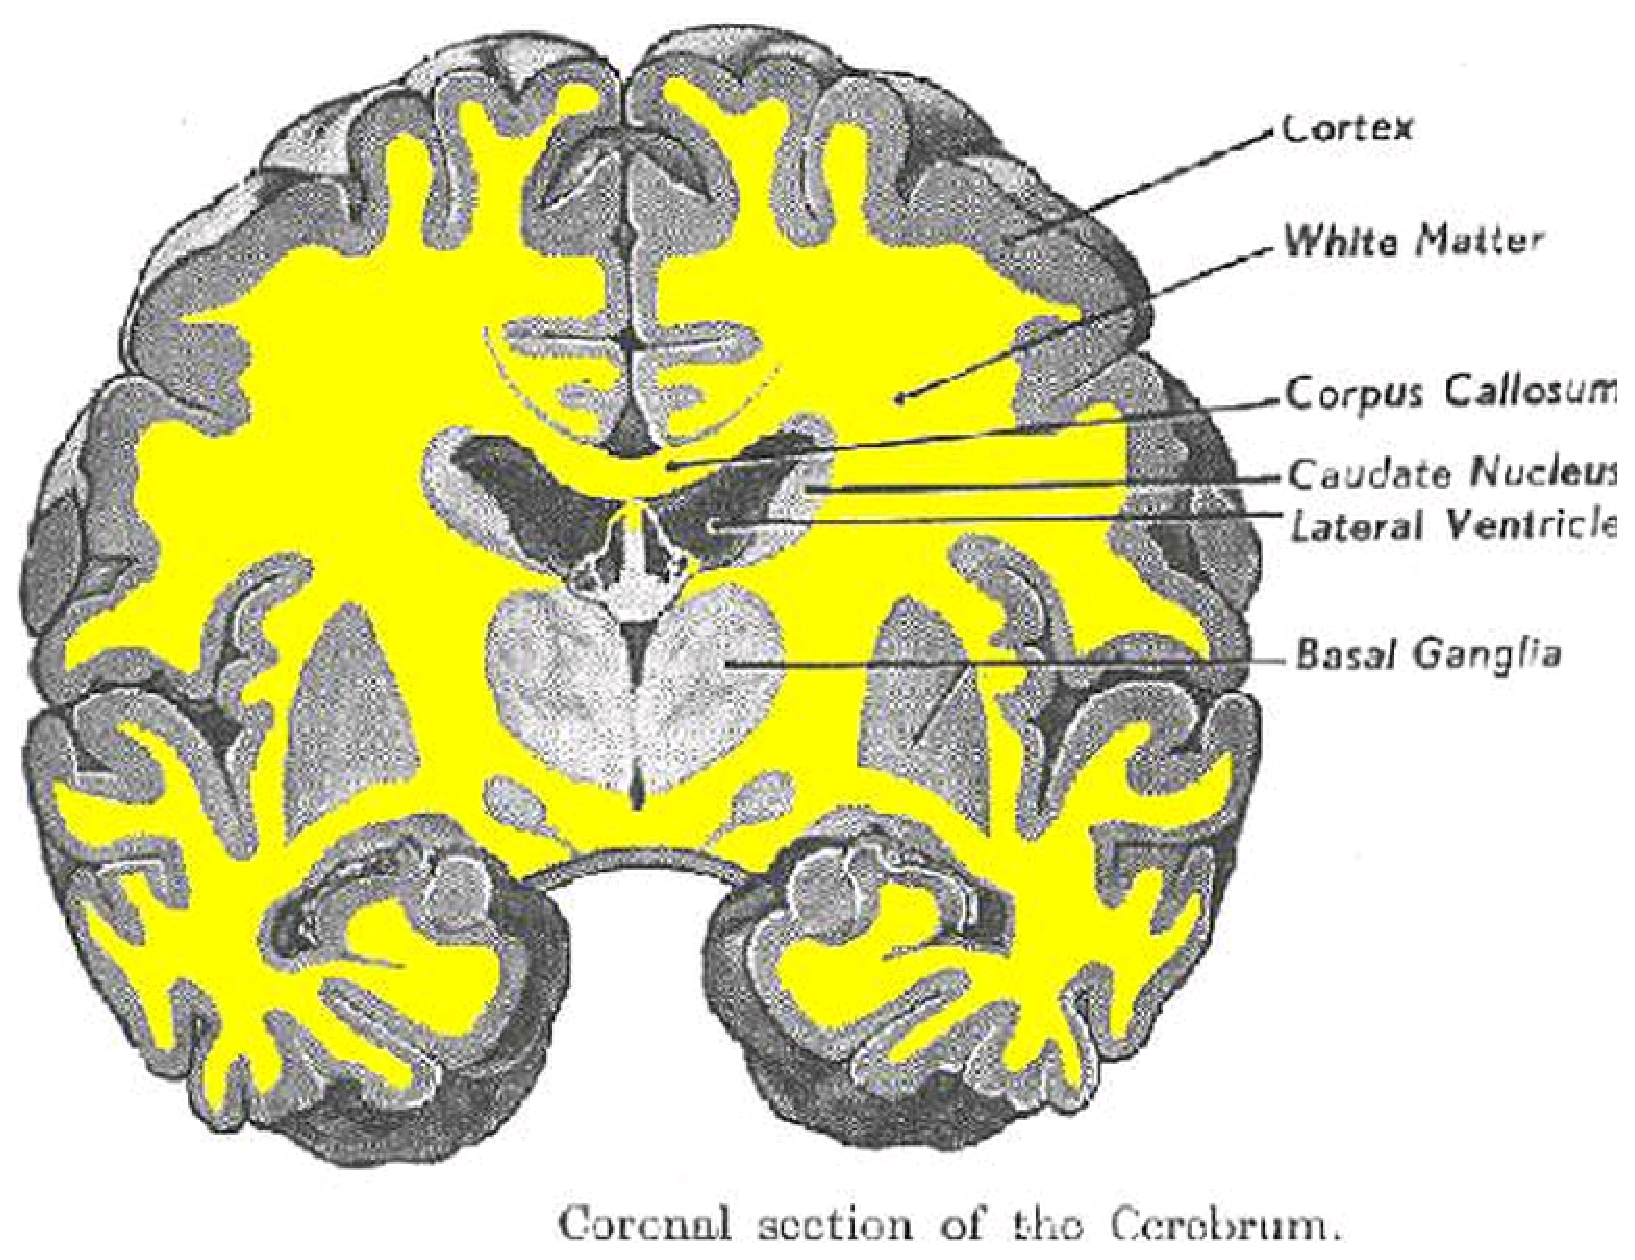
\includegraphics[height=4cm,
    angle=0]{./images/cerebrum_coronal_section.eps}}
  \caption{Cerebrum with 2 main parts: grey matter and white matter}
\label{fig:cerebrum_coronal_section}
\end{figure}


\section{1.A. Cerebral hemispheres}
\label{sec:hemisphere-brain}
\label{sec:brain-hemisphere}

The two hemispheres of the brain are connected by commissure fibers
(Sect.\ref{sec:commissural-fibers}).

The right side of the brain controls muscles on the left side of the body and
the left side of the brain controls muscles on the right side of the body.
Also, in general, sensory information from the left side of the body crosses
over to the right side of the brain and information from the right side of the
body crosses over to the left side of the brain. Therefore, damage to one side
of the brain will affect the opposite side of the body.
\footnote{\url{http://biology.stackexchange.com/questions/3807/why-do-the-two-hemispheres-of-the-brain-control-the-opposite-sides-of-the-body}}

It appears that the right brain is dominant for spatial abilities, face
recognition, visual imagery and music. The left brain may be more dominant for
calculations, math and logical abilities. Of course, these are generalizations
and in normal people, the two hemispheres work together.
\url{https://faculty.washington.edu/chudler/split.html}

We will study the cerebral hemispheres from 
\begin{enumerate}
  \item grey matter - Sect.\ref{sec:grey_matter}
  
  \item white matter - Sect.\ref{sec:white-matter-cerebrum}
\end{enumerate}

\section{* Cerebral cortex: neocortex (isocortex, cortex) +
allocortex + periallocortex}
\label{sec:cerebral_cortex}
\label{sec:grey_matter}
\label{sec:periallocortex}

The grey matter (or gray matter) is considered as the cortex of the cerebrum,
thus given the name {\it cerebral cortex} (Latin: {\it cortex } = "bark",
"rind", "shell" or "husk"). The cerebral cortex is part of the cerebrum
(Sect.\ref{sec:cerebrum}), beside white matter (Sect.\ref{sec:white-matter}).

Most of the cerebral cortex is {\bf neocortex} (Sect.\ref{sec:neocortex}); so
the terms are used interchangably.  However, there are phylogenetically older
areas of cortex termed the allocortex (Sect.\ref{sec:allocortex}).

The {\bf periallocortex} is the transitional zone between the neocortex and the
allocortex. So, we only focus on the neocortex (Sect.\ref{sec:neocortex}).


\subsection{Allocortex (heterogenetic cortex): archicortex, paleocortex}
\label{sec:allocortex}

Other parts of the cerebral cortex are: archicortex,
paleocortex, which are collectively called {\bf allocortex}
(Sect.\ref{sec:allocortex}).

{\bf Allocortex} (heterogenetic cortex) refers to the brain region comprised of
2 parts: the paleocortex, the archicortex; which forms the part of limbic system
- Sect.\ref{sec:limbic-system}.

The specific regions of the brain usually described as belonging to the
allocortex are 
\begin{enumerate}
  \item  archicortex: olfactory system - Sect.\ref{sec:olfactory-bulb}
  
  \item paleocortex: comprise the gyrus cinguli, hippocampal gyrus
  (Sect.\ref{sec:hippocampus}), and amygdala.
\end{enumerate}


Similar to neocortex, allocortex also have laminar structures; but less than 6
layers. Allocortex is characterized by having just three or four cell layers, in
contrast with the six layers of the neocortex, and takes up a much smaller area
than the neocortex. 

Allocortex is termed heterogenetic cortex, because during development it never
has the six-layered architecture of homogenetic neocortex.
It differs from {\it heterotypic cortex}, a type of cerebral cortex, which
during prenatal development, passes through a six-layered stage to have fewer
layers, such as in Brodmann area 4 that lacks granule cells.

\url{https://en.wikipedia.org/wiki/Allocortex}

\subsection{-- paleocortex}
\label{sec:paleocortex}

The paleocortex is part of the allocortex (Sect.\ref{sec:allocortex}). 

Paleocortex includes the piriform lobe (Sect.\ref{sec:piriform-cortex}),
specialized for olfaction, and the entorhinal cortex
(Sect.\ref{sec:entorhinal-cortex}).

\subsection{---- piriform cortex (perform lobe)}
\label{sec:piriform-cortex}

The piriform cortex sometimes called  olfactory cortex, olfactory lobe or
paleopallium; is related to sense of smell. It sends output to olfactory bulb.

\subsection{---- Entorhinal cortex (EC)}
\label{sec:entorhinal-cortex}

The {\bf entorhinal cortex} is a brain region part of paleocortex
(Sect.\ref{sec:paleocortex}). It is near the hippocampus and has direct
connections to it (Sect.\ref{sec:hippocampus}). This is the region first get
damaged in Alzheimer disease (AD, Sect.\ref{sec:Alzheimer-Disease}).

\subsection{-- archicortex}
\label{sec:archicortex}

The archicortex is part of the allocortex (Sect.\ref{sec:allocortex}).

The archicortex consists of the hippocampus (Sect.\ref{sec:hippocampus}), which
is a three-layered cortex dealing with encoding declarative memory and spatial
functions.


\subsection{Neocortex (isocortex, neopallium)}
\label{sec:neocortex}

% The mammalian neocortex of the forebrain (Sect.\ref{sec:forebrain}) is a
% structure with no equals in the vertebrates.

The neocortex (isocortex) comprises 90\% of the cerebral cortex
(Sect.\ref{sec:cerebral_cortex}). That's why some books use neocortex and
cerebral cortex interchangeably.
The neocortex (``neo'' = new) is the newest part of the forebrain
to evolve (Sect.\ref{sec:brain_evolution}).

It is 2-4 mm thick, at the top layer of the cerebral hemispheres; and has a
laminar structure with 6 distinctive (horizontally/radially) layers from outside
(pial surface) to inside (white matter) - Sect.\ref{sec:neocortex-6-layers}, and
tangentially subdivided into functional areas
(Sect.\ref{sec:neocortex_functional-column}). The detail is discussed in
Sect.\ref{sec:neocortex-details}.



% The details is covered in a separate section
% (Sect.\ref{sec:cerebellar_cortex_details}).

\begin{mdframed}

The folding structure of the grey matter allows a far more number of cortical
matter to be contained in a given-sized brain cavity.
In rodents, it is just a smooth surface, so it had long been wrongly accepted
that more intelligent people have more folded and grove surface. Indeed, the
white matters is the one that is more important (Sect.\ref{sec:white-matter}).

\end{mdframed}


If we looks from the exterior, it is divided into different {\bf lobes}
(Sect.\ref{sec:lobes}). The border between the lobes are anatomically marked by
the different {\bf sulci}.
\begin{enumerate}
  \item frontal lobe
  \item parietal lobe
  \item occipital lobe
  \item temporal lobe
\end{enumerate}


\begin{figure}[hbt]
  \centerline{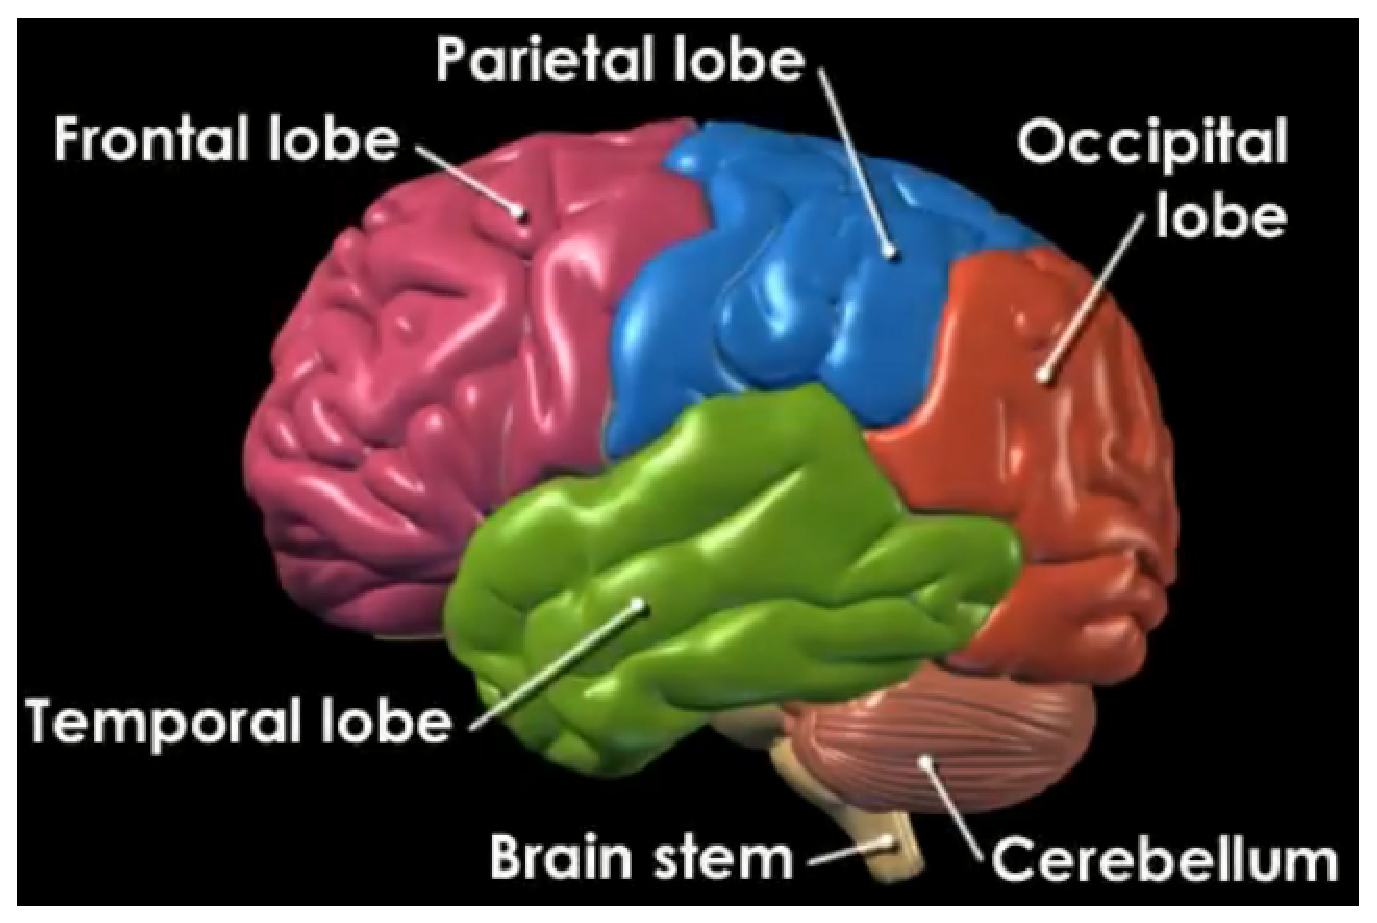
\includegraphics[height=4cm,
    angle=0]{./images/brain_02.eps},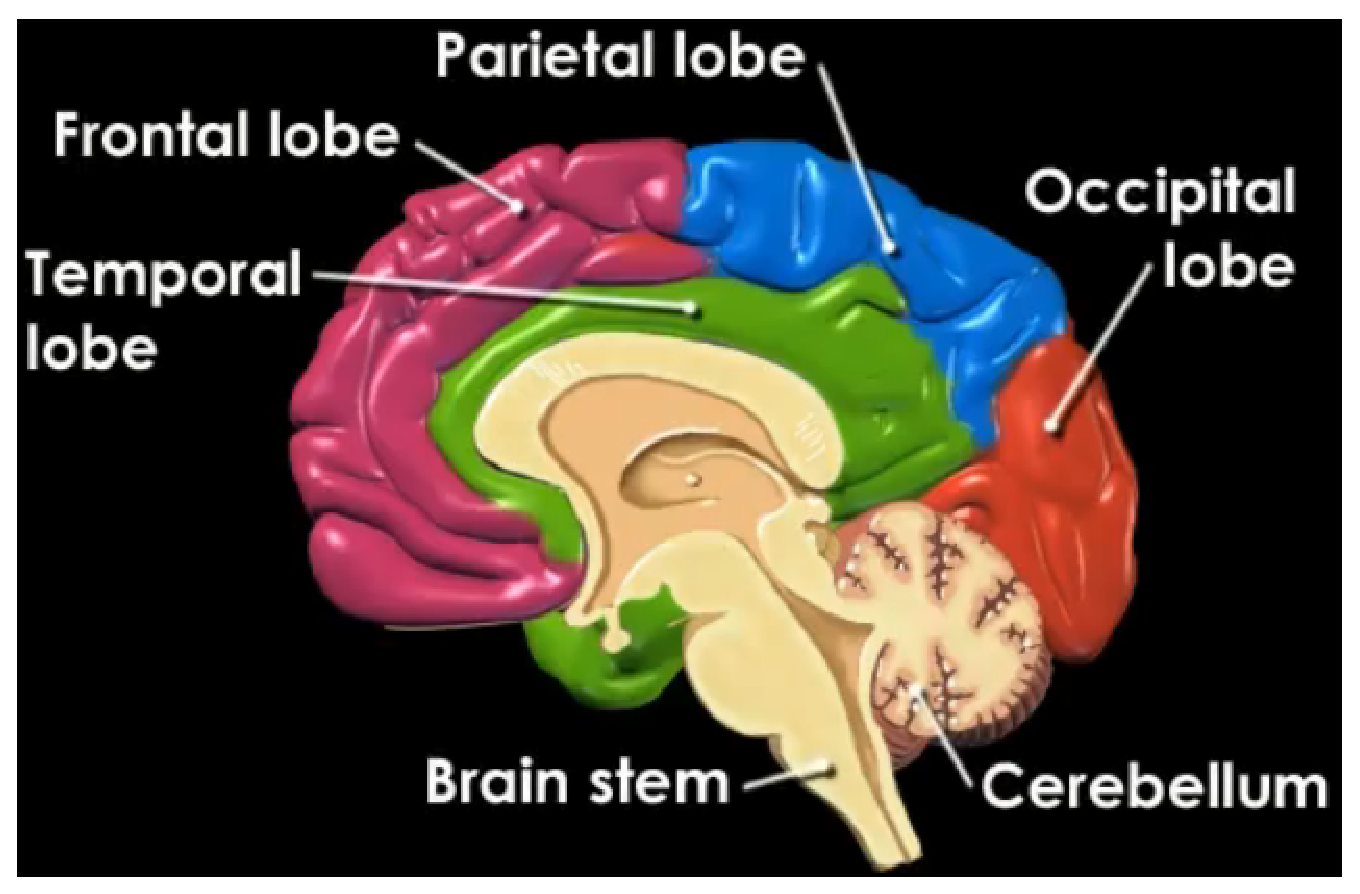
\includegraphics[height=4cm,
    angle=0]{./images/brain_03.eps}}
  \caption{Anatomical structure of the cerebrum (A) from front to back of the
  head, (B) cross-section view from front to back of the head. They are divided
  into regions (frontal lobe, parietal lobe, occipital lobe, temporal lobe,
  brain stem, cerebellum) by Sylvian fissure, central sulcus
    and parieto-occipital sulcus. All of the lobes are further subdivided by
    smaller sulci. }
\label{fig:cerebrum_lobes}
\end{figure}



\subsection{Pyramidal system}
\label{sec:pyramidal-system}

{\bf pyramidal system} refers to corticofugal neurons
(Sect.\ref{sec:corticofugal-projection neurons}) that give rise to corticospinal
projections. See also extra-pyramidla
system - Sect.\ref{sec:extra-pyramidal-system}.

\subsection{Summary}

Neurons from the cerebrum connects with neurons in other regions, with
the spinal cord, facilitating smooth, precise movement, controlling
balanced and
posture\footnote{\url{http://www.coheadquarters.com/coOuterBrain1.htm}}.
Though regions in the neocortex appear to be specialized to
participate in specific types of psychophysical functions, as shown in
Fig.~\ref{fig:functional_region}. It must be fully appreciated that no
single area in the brain has been successfully identified as the sole
functional area of any psycho-physical phenomenon. Rather, the brain
seems to have a highly distributed functionality with many different
regions (both cortical and non-cortical) making important contribution
to every such function.

\begin{figure}[hbt]
  \centerline{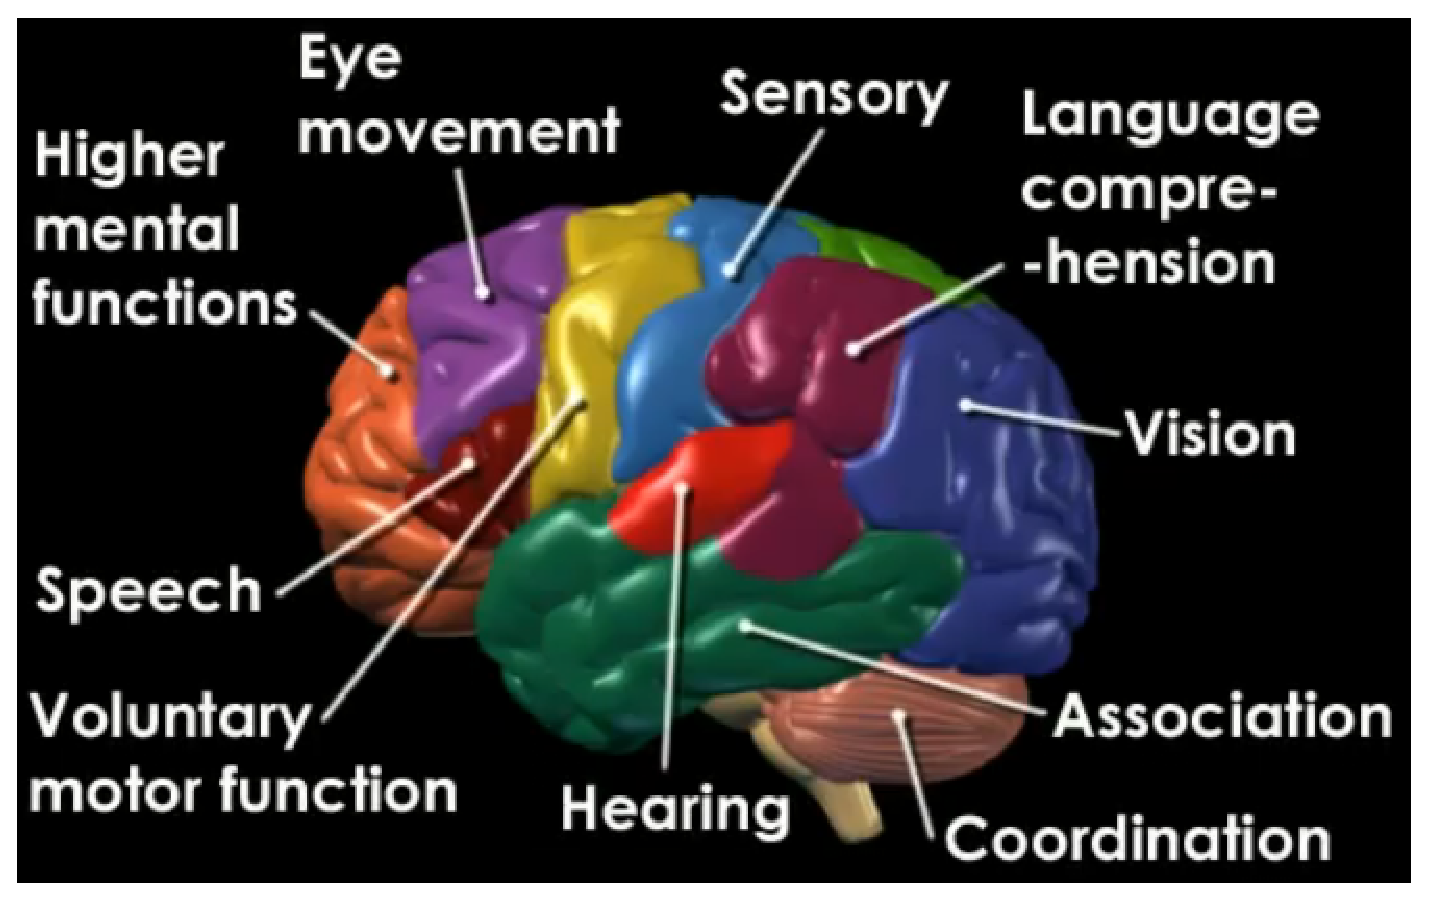
\includegraphics[height=4cm,
    angle=0]{./images/brain_06.eps},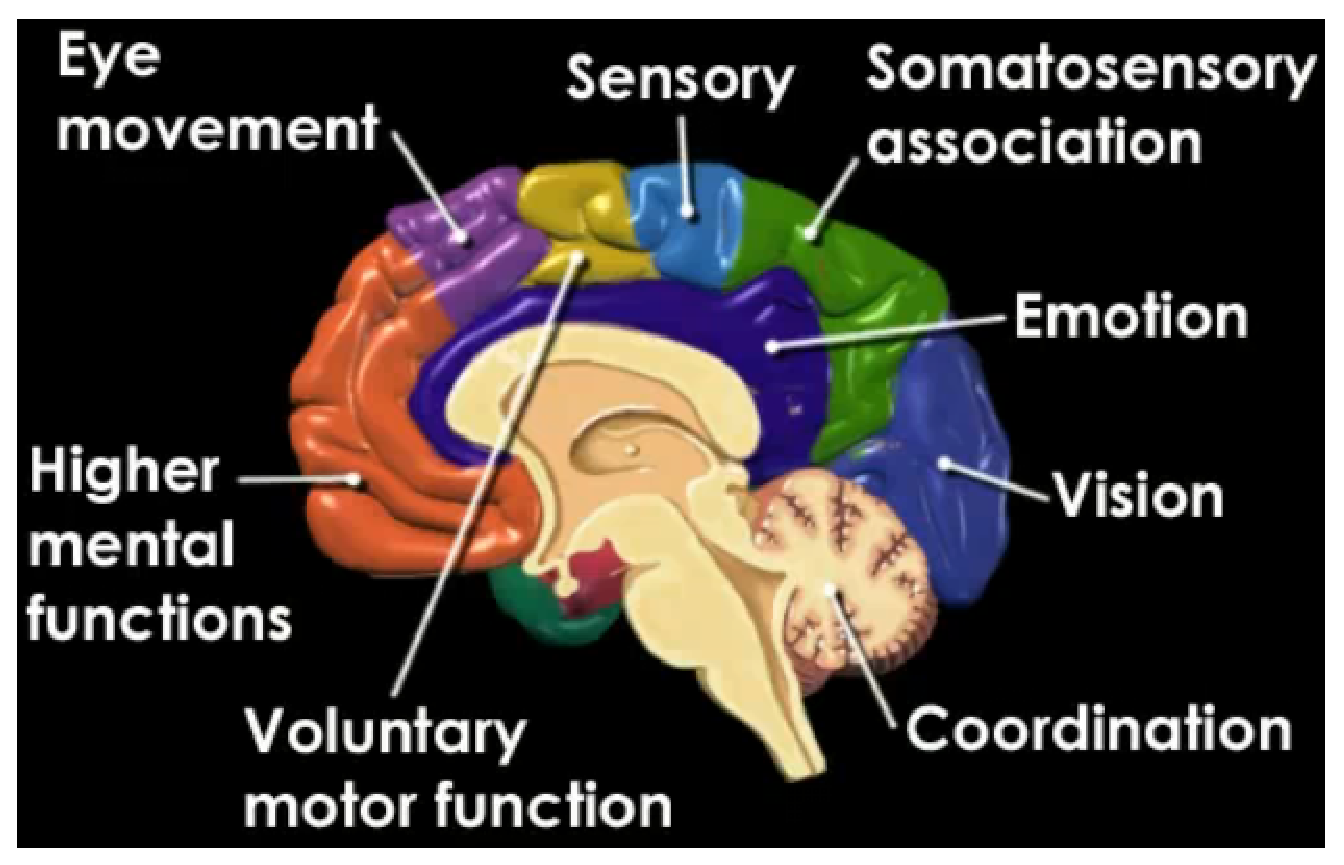
\includegraphics[height=4cm,
    angle=0]{./images/brain_07.eps}}
  \centerline{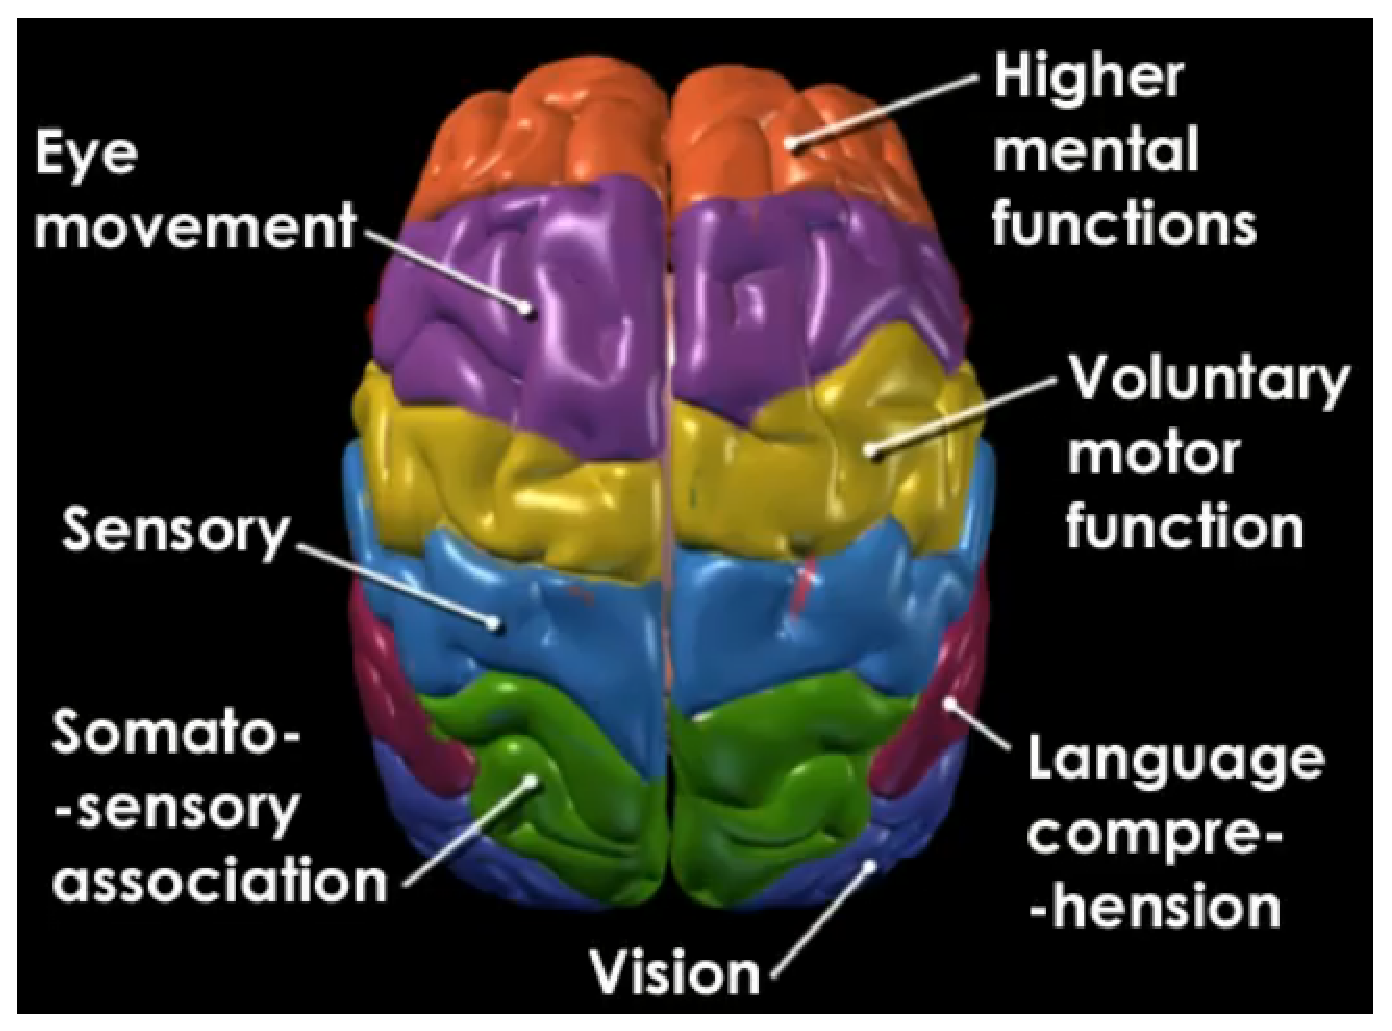
\includegraphics[height=4cm,
    angle=0]{./images/brain_08.eps},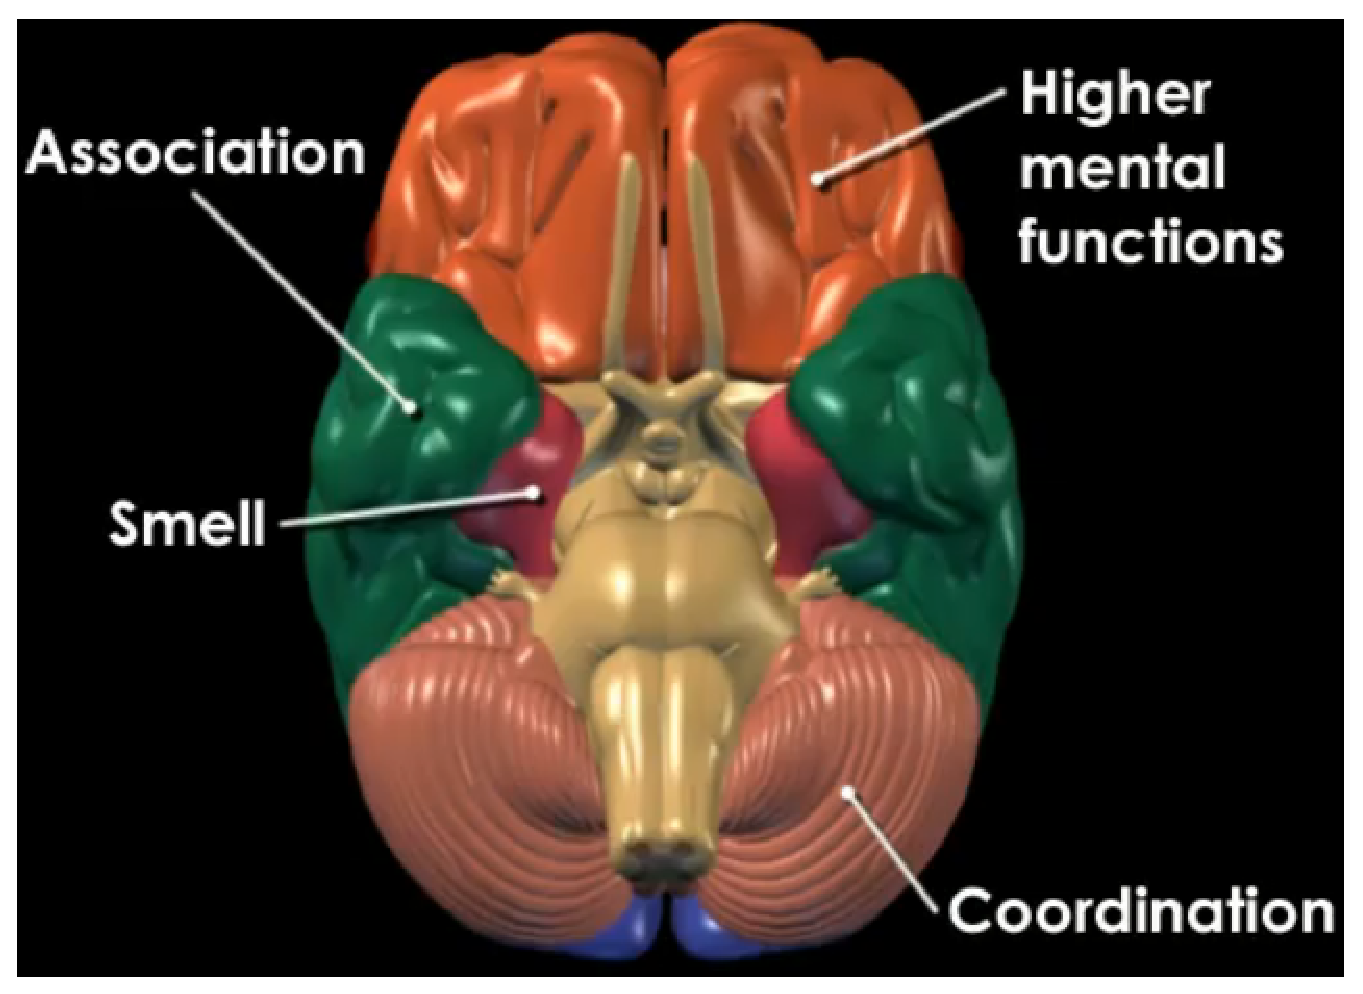
\includegraphics[height=4cm,
    angle=0]{./images/brain_09.eps}}
 \caption{Different functional regions in the brain}
\label{fig:functional_region}
\end{figure}

% \section{Cerebral cortex (details)}
% \label{sec:cerebellar_cortex_details}


\section{-- Neocortex (isocortex)}
\label{sec:neocortex-details}

In human, the thickness of the cerebral cortex (or neocortex to be precise) is
subject to regular local variations, but the average value is from 1.5 to 4.5 mm
(Brodmann, 2010) and is a heavily folded surface.

Neocortex is considered as  the most recently evolved part of the cortex
(Sect.\ref{sec:neopallium}). This section continues the discussion of neocortex
(Sect.\ref{sec:neocortex}).
\begin{itemize}
  \item Classify into gyrus: 
  
  \item Classify into lobes: anatomical view at the surface
  
  \item Classify into (horizontal) layers: from outside to inside
  
  6 layered structure (Sect.\ref{sec:layered_structure}) or 3 functional layers
  (Sect.\ref{sec:layered_structure-functional})
   
  \item Classify into (vertical) functional columns: regions in terms of
  functional role (Sect.\ref{sec:neocortex_functional-column})


\begin{itemize}
  \item motor cortex: Sect.\ref{sec:motor-cortex}
  \item somatosensory cortex - Sect.\ref{sec:somatosensory-cortex}
  \item auditory cortex - Sect.\ref{sec:auditory-cortex}
\end{itemize}
and different association areas as described in Brodmann's map
(Sect.\ref{sec:area_in_brain}).
\begin{itemize}
  \item parieto-occipitotemporal association area
  \item prefrontal association area
  \item limbic association area
  \item Broca's area
  \item Wernicke's area
\end{itemize}

  \item 

\end{itemize}



%there are 6 horizontal layers in the  neocortex 


\begin{mdframed}
{\it Corticocortial} = connecting one cortex with
another. {\it Afferent} = ascending pathway = carrying nerve signal from the
receptors or sense organs toward the CNS. {\it Efferent} = descending pathway = opposite of
afferent.

\end{mdframed}

\subsection{Sulcus (fissure) and Gyrus}
\label{sec:sulcus}
\label{sec:fissure}
\label{sec:gyrus}

As the neocortex of the human grows much faster than the skull, to be able to
hold the increased number of neurons in the brain's surface, the grey matter is
highly folded. Each fold (groove) is called {\bf sulcus} (pl. sulci - valley) or
{\bf fissure} - depending on its depth (fissure is a deep sulcus,
Fig.\ref{fig:cerebral_hemispheres}(B)).

Each surface ridge - the folded cortex between two adjacent sulci - is called
{\bf gyrus} (pl. gyri - ropy structure), Fig.\ref{fig:brain_cerebrum}, which
often take the form of elongated convolution. It is generally surrounded
by one or more sulci (depressions or furrows; sg. sulcus)


\begin{figure}[hbt]
  \centerline{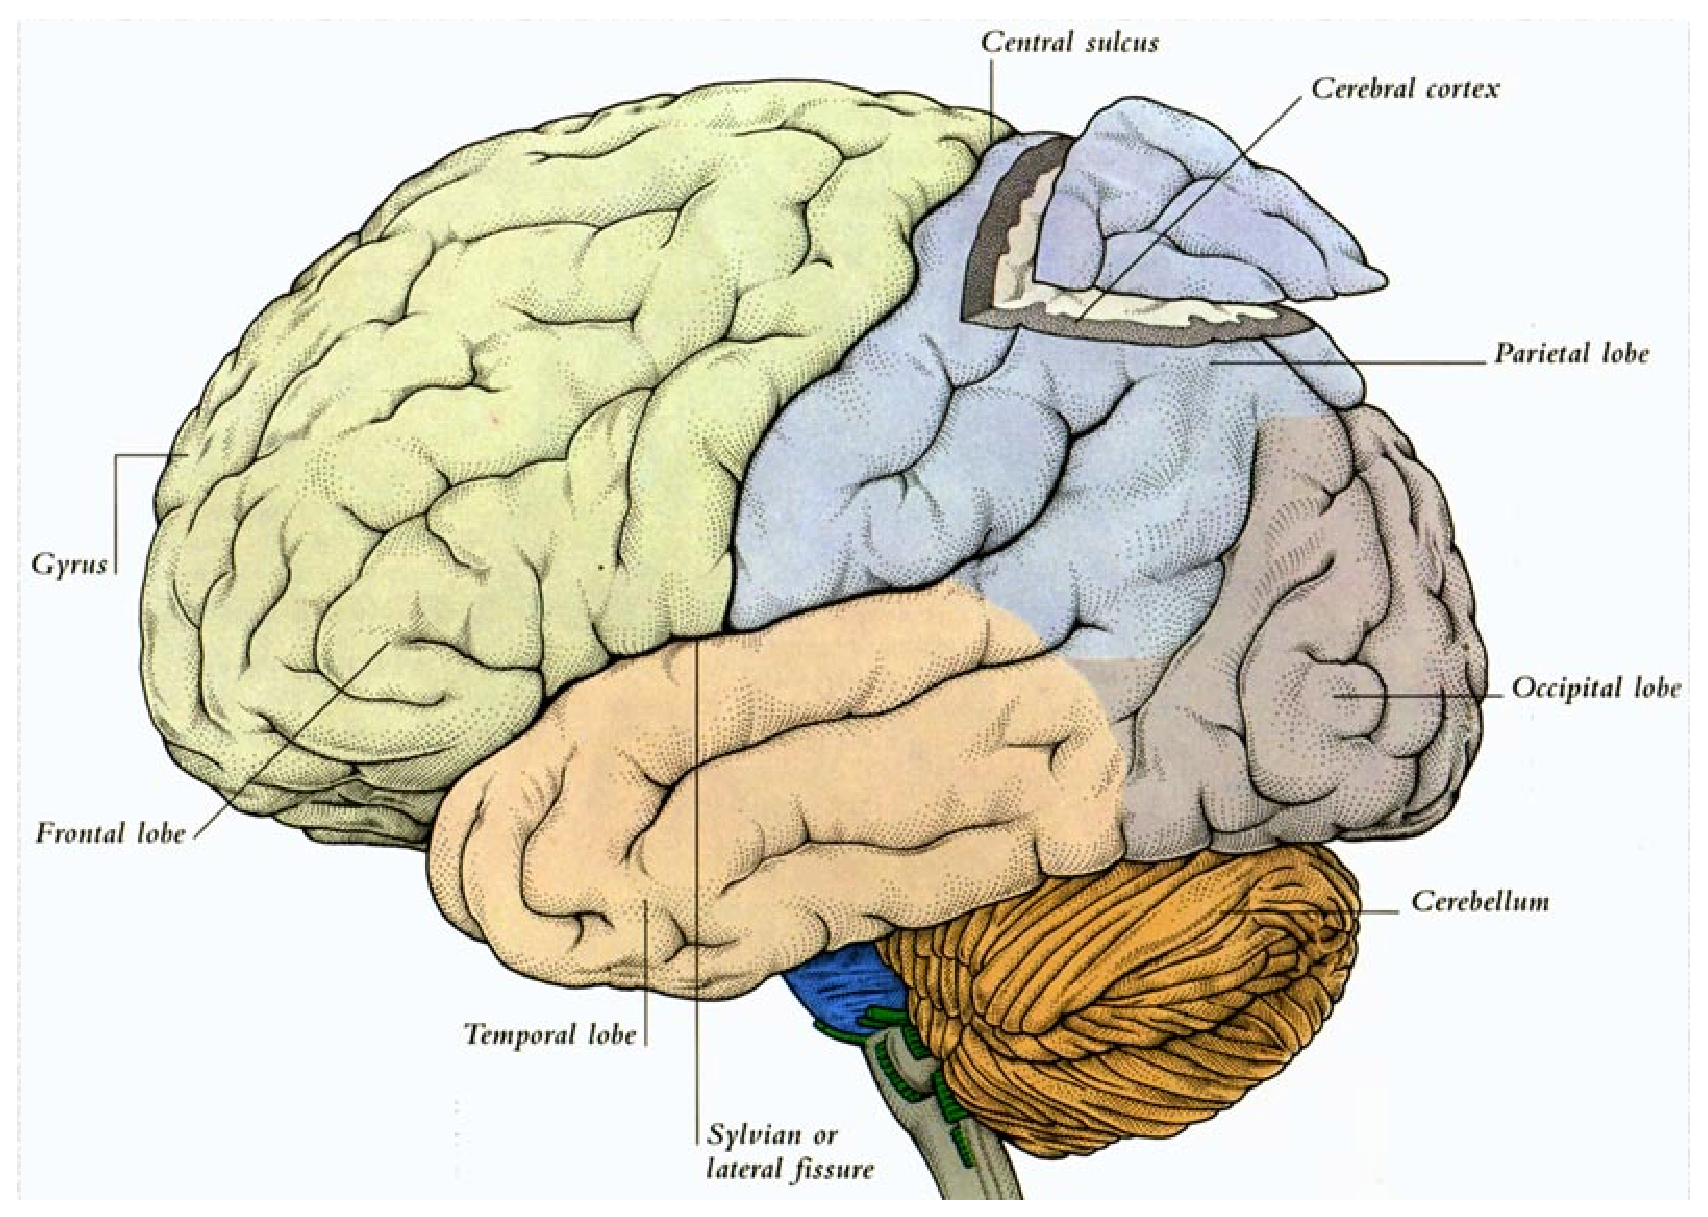
\includegraphics[height=8cm,
    angle=0]{./images/brain_11.eps}}
\caption{Outer brain surface in detail: gyrus, frontal lobe, central sulcus,
lateral sulcus (Sylvian fissure), cerebral cortex, parietal lobe, occipital
lobe, cerebellum}
\label{fig:brain_cerebrum}
\end{figure}

\begin{itemize}
  \item The two really large fissures are called {\bf Sylvia fissure} (lateral fissure,
some times called lateral sulcus as well) and {\bf Interhemispheric fissure}
(longitudinal fissure).

  \item There is another popular sulcus is {\bf central sulcus} (originally:
Rolandic Fissure). The sulci provide convenient landmark to help anatomists
classifying different regions of the neocortex, called {\bf lobe},
Fig.\ref{fig:cerebrum_lobes} (Sect.\ref{sec:lobes}).
\end{itemize}


%\subsection{* Cingulate cortex = Cingulate gyrus + Cingulate sulcus}
\subsection{* Cingulate gyrus: between cingulate sulcus and sulcus of corpus
callosum}
\label{sec:cingulate_gyrus}
\label{sec:cingulate_sulcus}
\label{sec:sulcus-corpus-callosum}

\begin{figure}[htb]
  \centerline{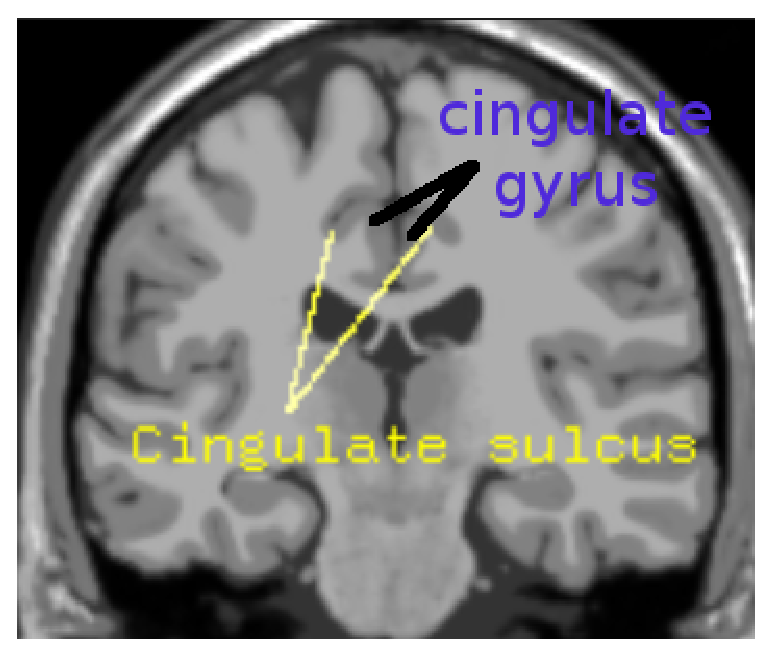
\includegraphics[height=6cm]{./images/cingulate-gyrus.eps}}
  \caption{Cingulate gyrus (the grey matter) and Cingulate
  sulcus}\label{fig:cingulate-gyrus}
\end{figure}

In between the two hemisphere, the grey matters fold deep into the inside the
brain, and the sulcus here is called {\bf cingulate sulcus}. The ridge formed by
the cingulate sulcus and the sulcus of the corpus callosum is called
{\bf cingulate gyrus}. The name {\it cingula} refers to the shape of the
region that looks like a 'belt' (or a zone)
\begin{itemize}
  \item cingulate gyrus
  \item cingulate sulcus
\end{itemize}

If we look from left to right, the {\bf cingulate gyrus} is an arched
convolution that lies immediately below the {\it cingulate sulcus}, and
immediately above the corpus callosum (Sect.\ref{sec:corpus_callosum}) and both
are separated by the sulcus of corpus callosum.

Some researchers belive cingulate gyrus is a part of the limbic system 
(Sect.\ref{sec:limbic-system}), while others think they not but are closely
linked .


\subsection{* Precentral gyrus}
\label{sec:precentral-gyrus}


{\bf Precentral gyrus} is the gyrus on the posterior frontal lobe.
It has other names, Fig.\ref{fig:cerebral_hemispheres}(A):
\begin{itemize}
  \item gyrus precentralis (Latin word)
  \item motor strip (English word)
  
  It is responsible for motor ability (Sect.\ref{sec:motor-cortex})
(which can be damanaged if a stroke occurs). The precentral gyrus on the left
hemisphere control the motion of the body's right side. 
   
  \item Jackson's strip (name after Hughlings-Jackson who noted it)
  
  \item primary motor cortex (or M1 - Sect.\ref{sec:M1-region}): used by
  electrophysiologists
  
  \item somatomor strip or motor homonculus (motor human)
\end{itemize}


\begin{figure}[htb]
  \centerline{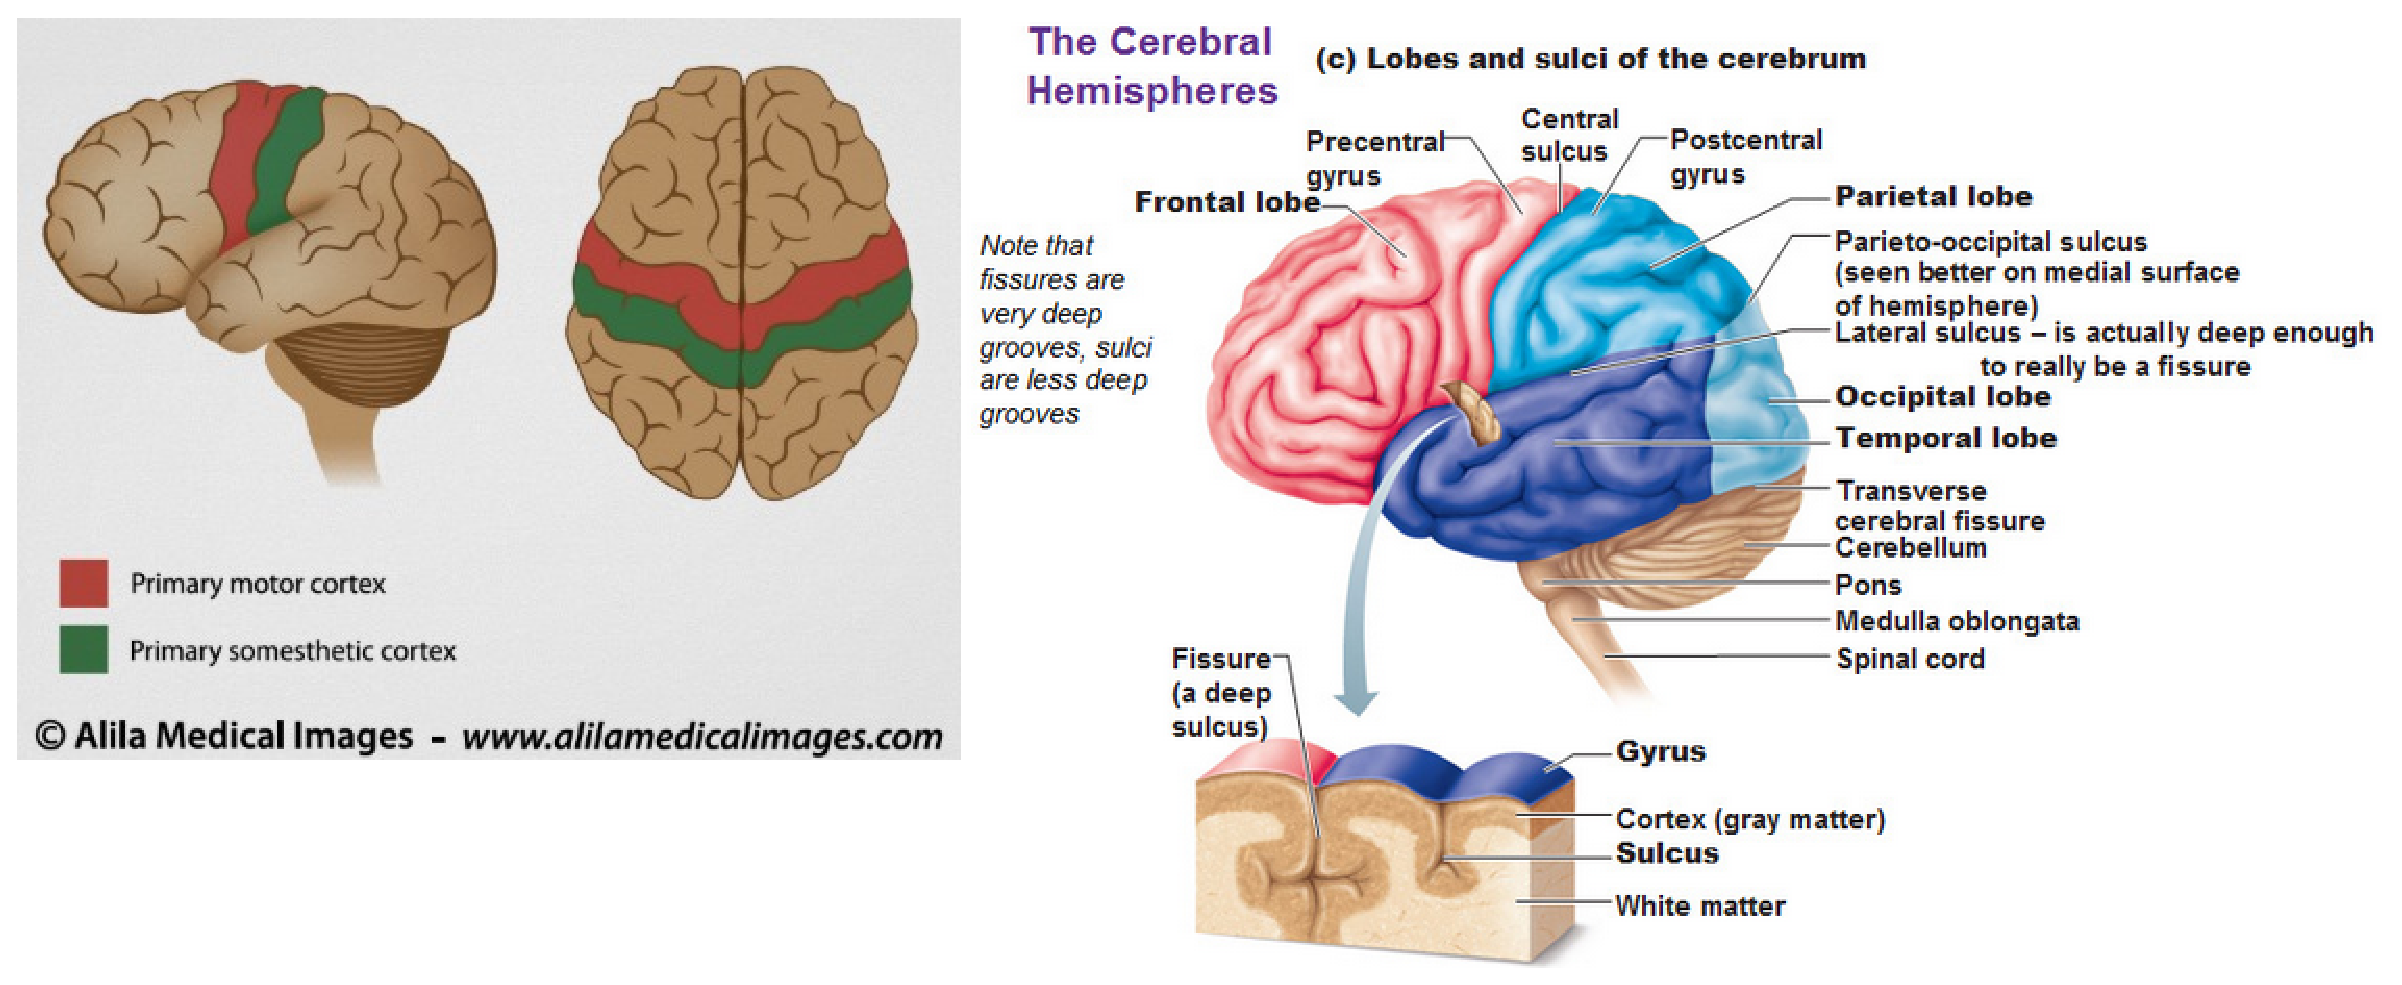
\includegraphics[height=6cm]{./images/cerebral_hemispheres.eps}}
  \caption{(A) precentral gyrus and postcentral
  gyrus; (B) fissure is deeper than sulcus}\label{fig:cerebral_hemispheres}
%http://antranik.org/the-cerebral-hemispheres/  
\end{figure}
 


\subsection{* Postcentral gyrus (contain primary somatosensory cortex)}
\label{sec:postcentral-gyrus}
\label{sec:somatosensory-cortex}

{\bf Postcentral gyrus} is a structure that forms a band around the middle of
the cerebral cortex, encompassing both hemispheres,
Fig.\ref{fig:cerebral_hemispheres}(A).
The postcentral gyrus is the primary sensory area
(Sect.\ref{sec:somatosensory-cortex}) and it preceives pain, touch, pressure,
and temperature.

Underneath of this gyrus is the is {\it primary somesthetic cortex} column, {\it
primary somatosensory cortex} column, or {\bf area 1, 2, 3} based on Brodmann
area (Sect.\ref{sec:Brodmann_area}). {\it Primary} in this case means that a
hierarchy of cortical areas is assumed in which the initial processing of
tactile information is continued in secondary (S2) and so forth "higher"
somatosensory areas.


The somatosensory cortex is organized into regions, such that each hand digit
maps to a specific region. Neurons within each region are organized into tight
clusters called neuronal groups, such that synaptic weights between neurons
within a neuronal group is significantly higher than weights between neurons in
different groups. This group structure is hypothesized to arise as a consequence
of self-organization through synaptic changes driven by the sensory input.



\subsection{Lobes}
\label{sec:lobes}

There are totally 4 lobes: {\bf frontal lobe}, {\bf temporal lobe}, {\bf
occipital lobe}, and {\bf parietal lobe}, as shown in
Fig.~\ref{fig:cerebrum_lobes}.
Lateral sulcus (Sylvian fissure, lateral fissure) - one of the earliest
developing sulcus of the human brain: divides both the frontal lobe and parietal
lobe from temporal lobe. The lateral sulcus is in both hemisphere, but it is
longer in the left hemisphere in most people.

\subsection{-- Frontal lobe}
\label{sec:frontal-lobe}

{\bf Frontal lobe}, in humans, reach its full maturity only after the
20s. This part contains most of dopamine-sensitive neurons which are
associated with emotion, attention, long-term memory, planning and
skilled-movement (e.g. drive). 

The frontal lobe is divided into the prefrontal cortex
(Sect.\ref{sec:prefrontal-cortex}) and the posterior frontal lobe in which
precentral gyrus is the prominent structure (Sect.\ref{sec:precentral-gyrus}).

\subsection{-- Parietal lobe}
\label{sec:parietal-lobe}
\label{sec:posterior-lobe}

{\bf Parietal lobe} integrate sensory information, perceiving and interpreting
bodily sensations (i.e. touch, pressure, pain, temperature). Its name derives
from the overlying parietal bone (Latin: {\it pariet}- = wall).

The central sulcus separates the frontal lobe (Sect.\ref{sec:frontal-lobe}) from
the parietal lobe.


\subsection{-- (Medial) Temporal lobe (temporal area)}
\label{sec:temporal-lobe}

The {\bf (medial) temporal lobe} involves in auditory processing (recognition
of specific tones and loudness) and play key roles in long-term memory
storage
(Sect.\ref{sec:long-term_memory})\footnote{\url{http://www.neuroskills.com/tbi/btemporl.shtml}}

The {\bf left temporal lobe} holds the primary auditory cortex.
Left temporal lesions result in impaired memory for verbal material.
Left temporal lesions disturb recognition of words, i.e. memory of names (names
of people, names of animals, names of tools), live in the left temporal
lobe\footnote{\url{http://www.psycheducation.org/emotion/temporal names.htm}}.

The {\bf right temporal lobe} has many different functions that complement left
temporal lobe functions. The major functions of the right temporal lobe are
nonverbal memory, nonverbal aspects of communication (memory for pictures,
visual scenes, familiar faces, routes or directions and music), but may also
contribute to verbal memory (i.e. aspects of pitch and sound location) and
certain aspects of personality. Right side lesions result in recall of
non-verbal material, such as music and drawings.
% Right temporal damage can cause a loss of inhibition of talking.
\footnote{\url{http://oureverydaylife.com/right-temporal-lobe-functions-35962.html}}

The medial temporal lobe consists of structures that are vital for declarative
or long-term memory (Sect.\ref{sec:declarative-memory}). This includes: the
hippocampus, along with the surrounding hippocampal region consisting of the
perirhinal, parahippocampal, and entorhinal neocortical regions.


% Annu Rev Neurosci. 2004;27:279-306.
% The medial temporal lobe.
% Squire LR1, Stark CE, Clark RE.

\subsection{-- Occipital lobe}
\label{sec:occipital-lobe}

{\bf Occipital lobe} contains most of the anatomical region of the
visual cortex (i.e. detect and interpret visual images).
Fig. \ref{fig:cerebrum_views} shows different angles of view of the
Cerebrum.

\begin{figure}[hbt]
  \centerline{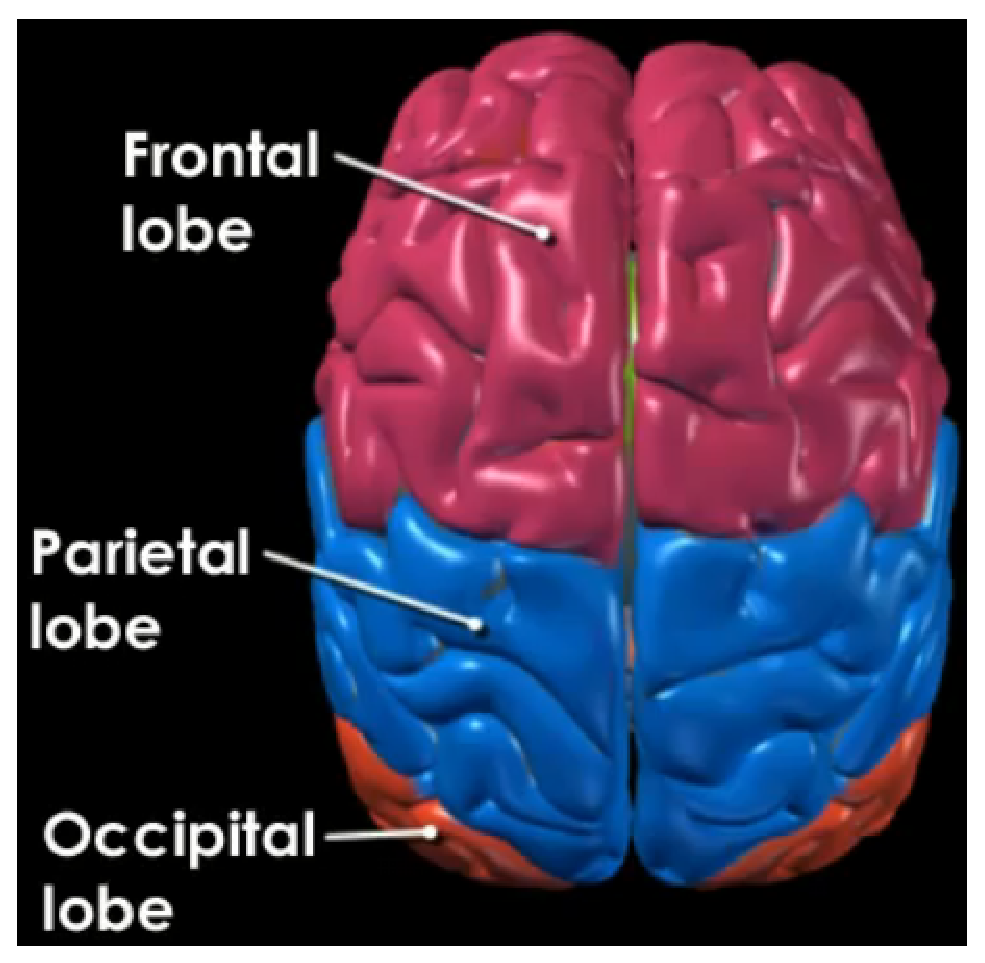
\includegraphics[height=4cm,
    angle=0]{./images/brain_04.eps},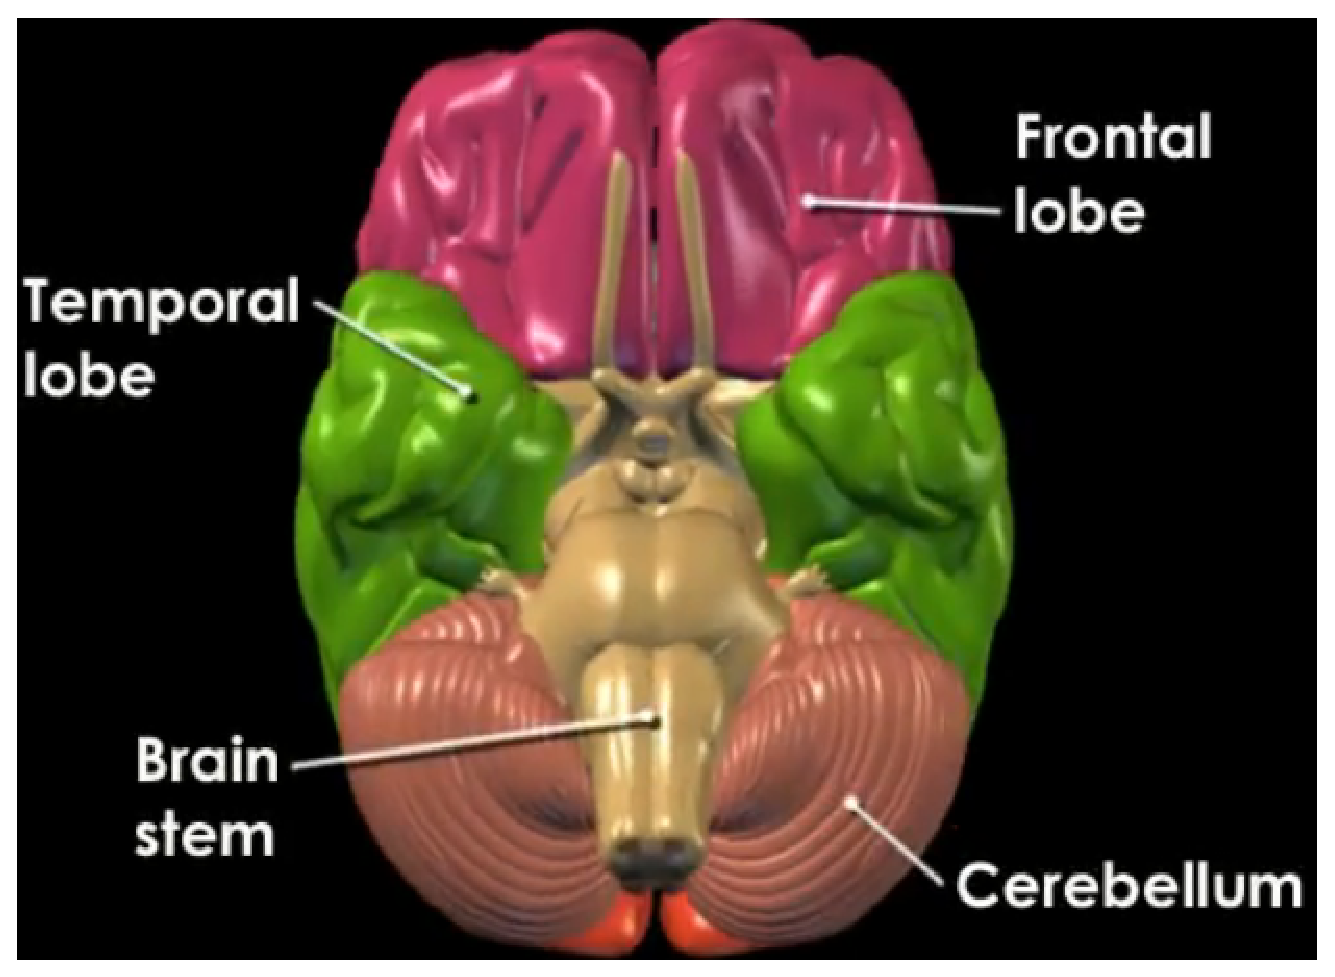
\includegraphics[height=4cm,
    angle=0]{./images/brain_05.eps}}
\caption{Different views of the cerebrum}
\label{fig:cerebrum_views}
\end{figure}

\subsection{Primary cortices (vertical functional columns): M1, V1, A1, S1}

Certain cortical regions have somewhat simpler functions, termed the primary
cortices.  These regions directly receive sensory input (vision, hearing,
somatic sensation) or directly involved in production of limb or eye movements.

\textcolor{red}{In essence, it's very difficult to determine the exact
  connectivity of neurons in the neocortex.}
Thus, some researchers prefer to refer to neocortical interconnection as
`random'; yet there are some simple rules they follows~\cite{well2005cnc}.
Tangentially, there are 4 primary functional columns
\begin{itemize}
  \item [1] motor cortex column (M1): control movement -
  Sect.\ref{sec:M1-region}.

  \item [2,3,4] The three below columns are called {\it sensory areas}.
  \begin{enumerate}
    \setcounter{enumi}{2}
%     (If you have lists at deeper levels of nesting, the relevant counters are
%     enumii, enumiii and enumiv.)
  \item visual cortex column (V1) : input from eye/retina (Chap.\ref{chap:Retina})

  \item auditory cortex column (A1): input from inner ear/cochlea

  \item primary somatosensory (associative) cortex column (S1): input from whole
  body, i.e. from exteroceptors (nociceptors, thermoreceptors and mainly
  mechanoreceptors). Sect.\ref{sec:somatosensory-cortex}
\url{http://www.scholarpedia.org/article/S1_laminar_specialization}
  
  S1 area has a very well-developed layer IV and is thus widely used to
  study.
  \end{enumerate}
\end{itemize}

However, the impressive plasticity of the neocortex, which is able to rewire and
reorganizeareal structures and connectivity after impairments ofsensory
pathways, argues for a more complex scenario \citep{alfano2013}.

The neurons within a given column are stereotypically interconnected in the
vertical dimension, share extrinsic connectivity, and hence act as basic
functional units subserving a set of common static and dynamic cortical
operations that include not only sensory and motor areas but also association
areas subserving the highest cognitive functions.

\subsection{-- M1 region (primary motor cortex - brain area 4)}
\label{sec:M1-region}

M1 region receives input from striatum, cerebellum and sensory information -
through corticocortical connections, and from the {\it sensory areas} 
  
M1 (brain area 4) is the main contributor to electrical impulse passing down to
the spinal cord that control the execution of movement are generated in the
primary motor cortex. These impulses pass via the internal capsule to the
spinothalamic tract in the spinal cord, both parts of the pyramidal system.


\subsection{-- V1 region (primary visual cortex): striate region}
\label{sec:V1-region}

V1 is the simplest, earliest cortical visual area (Sect.\ref{sec:visual-cortex})
as is considered essential part of the brain for all species. It is highly
specialized for processing information about static and moving objects and is
excellent in pattern recognition, with 6 functionally distinct layers
(Sect.\ref{sec:layered_structure}).
\begin{itemize}
  \item Layer 4 receives the most visual input from the lateral geniculate
  nucleus (LGN), so is divided into 4 layers:  4A, 4B, 4C$\alpha$, and
  4C$\beta$.
  
  \item {\bf retinotopy}: in humans, the upper bank of the calcarine sulcus
  responds strongly to the lower half of visual field (below the center), and
  the lower bank of the calcarine to the upper half of visual field -
  Sect.\ref{sec:retinotopy}.

  
  \item 
\end{itemize}

Neurons in V1 display striped pattern
(Sect.\ref{sec:ocular-dominance-column}). The average number of neurons in the
adult human primary visual cortex, in each hemisphere, has been estimated at
around 140 million.


\subsection{neural types in neocortex (cerebral cortex)}

\textcolor{red}{Neural types}: Grey matter (cerebral cortex) has two primary
types of neurons: inhibitory interneurons ($\; \sim\;
20\%$ - Sect.\ref{sec:inhibitory-cell}) and excitatory pyramidal neurons
(Sect.\ref{sec:pyramidal-neurons}) ($\;\sim\; 80\%$). 

\subsection{Horizontal columns: 6 structural layer?}
\label{sec:layered_structure}
%\subsection{Layers}
\label{sec:neocortex-6-layers}
\label{sec:horizontal-columns}

The visual appearance of the cortex, through the cortical slice, shows different
patterns as it is composed of different layers. {\bf Layered structure} is found
in the cerebral cortex (Sect.\ref{sec:cerebral_cortex}) and cerebellar cortex
(Sect.\ref{sec:cerebellar_cortex}). This is the distinguish feature only found
in mammals, giving it the name 'neo' - the latest evolutionary part of the
brain.

This same pattern of lamination is seen in different neocortical areas in a
given species, as well as in necortices in different mammals.
\textcolor{red}{This suggests all pieces of cortex perform basically the same
type of transactions on the information they receive; and what defines the
difference is the number of transactions that can be carried}.

\textcolor{red}{How many structural layers?}: The widely used definition of
\textcolor{red}{6 layers is not accurate}, due to a historical mistake that 6
layers could be observed at 6 months of the cortex. Even 6 layers concept is
widely used, it is important to know that at different regions in the cortex, we
can have fewer layers.

Besides the 6 horizontal laminae (layers), sublaminar divisions are also
present.  However, there is no hard border between them, yet there being a
gradient of change of varying distinctiveness between many of them.
These gradients of change are brought about by the arrangement of structures
that are invisible in classic Nissl-stained sections, and these structures tend
to disperse the somata of the neurons found in that layer. It is clearly see
this phenomenon in the motor cortex, where the small neurons of layer IV,
visible in the fetal animal, become so dispersed by the growth of the enormous
dendrites of layer III and layer V pyramidal neurons that the layer IV of motor
cortex appears to have disappeared in the adult.

Each layer has a different composition in terms of neuron types and
connectivity. \textcolor{red}{Interestingly, a natural starting place
is layer 4, the layer in which sensory input first arrives}.
In cerebral cortex, recent molecular studies offer a glimpse into a much
richer stratification, which has hundreds of different neural cell types
(Sect.\ref{sec:cortical-neurons}) and a diverse range of glial cells
\citep{lein2007, molyneaux2007}.
During the last few years there has been remarkable progress in the discovery of
genes that identify distinct neuronal subtypes and control neuronal subtype
development.
Fig.\ref{fig:neocortical-genes} shows the distribution of different genes
(layer-specific genes) at different layers of the neocortex.

\begin{figure}[htb]
  \centerline{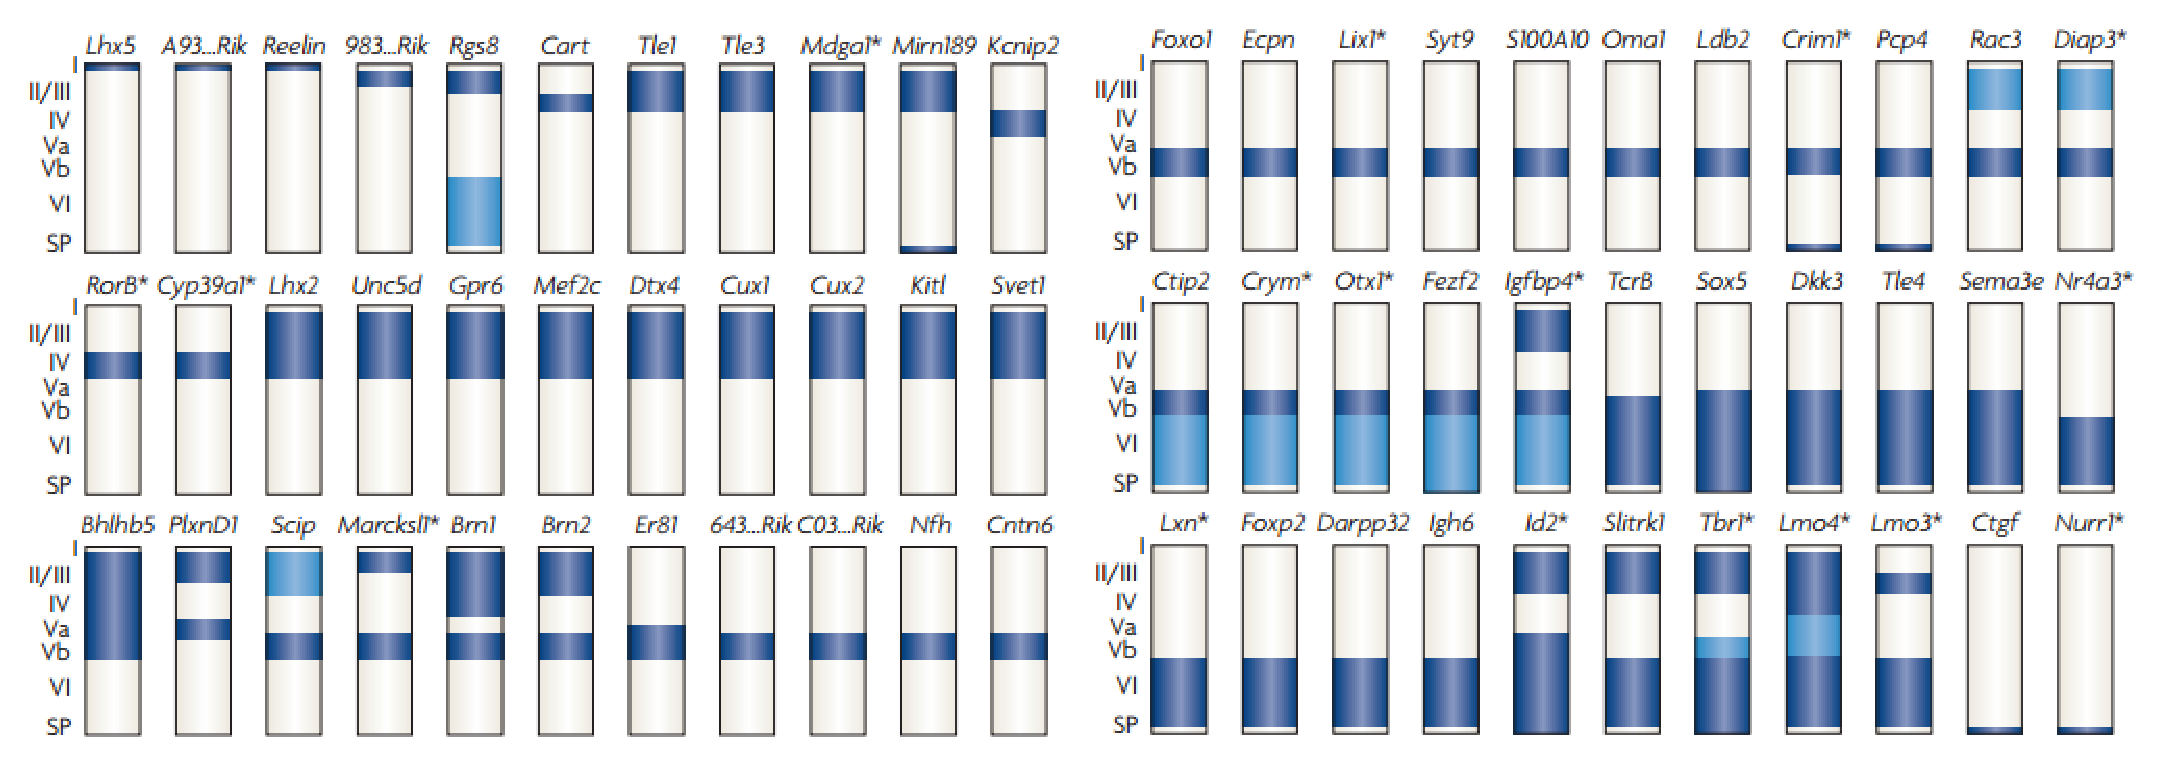
\includegraphics[height=5cm]{./images/neocortical-genes.eps}}
  \caption{Subtype genes in the mouse neocortex}\label{fig:neocortical-genes}
\end{figure}

\begin{itemize}
  \item pyramidal neurons (Sect.\ref{sec:pyramidal-neurons}): principal neurons
  in layer III (Sect.\ref{sec:layer-III}) and layer V (Sect.\ref{sec:layer-V}).

  \item GABAergic inhibitory interneurons:
  
In all layers, a complimentary set of GABAergic inhibitory interneurons can be
found, that are too diverse in form and function to shortly integrate them into
this summary.
  
  \item Spiny stellate cells : Sect.\ref{sec:stellate_cells}
  
  \item astrocytes:
  homogeneous distributed throughout the six-layered cortical organization
\end{itemize}
The neurons in these different layers connect vertically to form small
microcircuits. \textcolor{red}{These cortical microcircuits are grouped into
cortical columns and minicolumns} (Sect.\ref{sec:neocortex_functional-column}).

\subsection{** Layer I}
\label{sec:layer-I}

{\bf Layer I} (molecular layer): all kinds of input reaches this area via
synaptic conjunctions. So, this layers contains a dense connectivity matrix with
the dendrites of pyramidal neurons from deeper layers and very few horizontally
oriented neurons as well as glial cells - Sect.\ref{sec:glial-cells}.
\begin{enumerate}
  \item apical dendritic tufts of CPNs 
  \item horizontal axons of ??? (which neurons from which layers)
  \item Cajal-Reizius (Sect.\ref{sec:Cajal-Reizius-cell}) and 
  \item spiny stellate cells - Sect.\ref{sec:stellate_cells}
  \item astrocytes
\end{enumerate}

% ; and those
% it does contain are inhibitory neurons.

  
\subsection{** Layer II}
\label{sec:layer-II}

{\bf Layer II} (external granular layer) contains mostly 
\begin{enumerate}
  \item small pyramidal
cells (Sect.\ref{sec:pyramidal-neuron-layer-II}), 

  \item numerous stellate neurons
(Sect.\ref{sec:stellate_cells}) and 

  \item apical dendrites from pyramidal neurons in Layer V + VI
  (Sect.\ref{sec:pyramidal-neuron-layer-Va}).

  \item astrocytes
\end{enumerate}
  
Layer II is often pooled with layer III, i.e. layer II/III, due to the lack of a
clear between the two layers.
  
\subsection{** Layer III}
\label{sec:layer-III}

{\bf Layer III} (external pyramidal layer) contains a variety of cells,
mostly small and medium sized pyramidal cells. (Ichinohe,2012)
\begin{enumerate}
  \item large and robust CPNs (Sect.\ref{sec:pyramidal-neuron-layer-III})
  \item interneurons
  \item astrocytes
\end{enumerate}

\subsection{** Layer IV}
\label{sec:layer-IV}


Layer IV is most prominent in the primary sensory cortices. Layer IV is
prominent in the sensory cortex, and it is the primary recipient of afferent
connections from thalamus (type C neurons), i.e.
thalamocortical connection, \citep{miller2001} and from other cortical regions,
and sends the signals to other layers.

\textcolor{red}{Motor cortex lacks layer IV}. Cortical
  areas that lack a layer IV are called agranular. Cortical areas that have only
  an extremely small (or non-existent internal granular layer) layer
  IV are called {\bf dysgranular cortex} (agranular cortex).
\url{http://www.scholarpedia.org/article/S1_laminar_specialization}

{\bf Layer IV} (internal granular layer): 
\begin{enumerate}
  \item characterized by a very cell-dense appearance, mainly contain spiny
  stellate cells (Sect.\ref{sec:stellate_cells}) and 
  
  \item star-shaped pyramidal cells - Sect.\ref{sec:pyramidal-neurons}.
  
  \item densely packed polymorphous granulle cell
  (Sect.\ref{sec:granule_cells}):
  receive inputs from the thalamus and send projections to supragranular layers 2-3, but
  also to infragranular layers of the cerebral cortex.
  \item astrocytes
\end{enumerate}

Response tuning of layer 4 cells is largely determined by a local interplay of
feed-forward excitation (directly from the thalamus) and inhibition (from layer
4 inhibitory interneurons driven by the thalamus).

\begin{mdframed}

The studies often use the electrical signal regenerated from {\it whisker} -
long hair like growing from rat mouth.
The electrical message from the whisker follicle shoots up a pathway to an area
of the brain called the {\bf barrel cortex} - a dark-staining region of layer
IV of the somatosensory cortex. The barrel cortex that receives the signal
from whisker is called {\it whisker barrel}. The barrel cortex takes up a large
part of the somatosensory area of the rat's brain, the area that deals with touch.
\url{http://www.ratbehavior.org/RatWhiskers.htm}

\url{https://en.wikipedia.org/wiki/Barrel_cortex}
\end{mdframed}  



\subsection{** Layer V}
\label{sec:layer-V}


{\bf Layer V} (internal pyramidal layer) contains mainly the largest pyramidal
cells; along with basal dendrites of neurons in Layer III + VI.
\begin{enumerate}
  \item Layer Va pyramidal neurons: Sect.\ref{sec:pyramidal-neuron-layer-Va}
  \item Layer Vb pyramidal neurons: Sect.\ref{sec:pyramidal-neuron-layer-Vb}
  
  \item Betz cell: the giant pyramidal cells within layer V of primary
motor cortex
  \item astrocytes
\end{enumerate}

Pyramidal cells in layer V project long axons that leave the cortex and descend
to the subcortical structures (e.g.  basal ganglia). There are also Betz cells
whose axon travels through internal capsule, brain stem, and spinal cord,
forming the main pathways for voluntary motor control
(Sect.\ref{sec:pyramidal-neurons}).

\subsection{** Layer VI}
\label{sec:layer-VI}

{\bf Layer VI} (polymorphic or multiform or fusiform layer) contains different
neurons blending into the white matter; along with basal dendrites of
neurons from Layer III +  IV.

Major neurons found
\begin{enumerate}
  \item large CPNs
  \item small spindle-like pyramidal (fusiform neurons):
  
fusiform neurons = neurons with elongated soma; though it does not refer to a
uniform class of neurons, but can be a mixtured of deformed pyramidal neurons,
smooth stellate cells and Martinotti cells.
  
  \item astrocytes
\end{enumerate}


\subsection{-- 3 functional layers}
\label{sec:layered_structure-functional}

\textcolor{red}{How many functional layers?}: The 6 horizontal layers of the
cerebral cortex are organized into: supragranular layer (I to III), internal
granular layer (IV), infragranular layer (V and VI), as shown in Fig.~\ref{fig:laminal}.

\begin{figure}[hbtp]
  \centerline{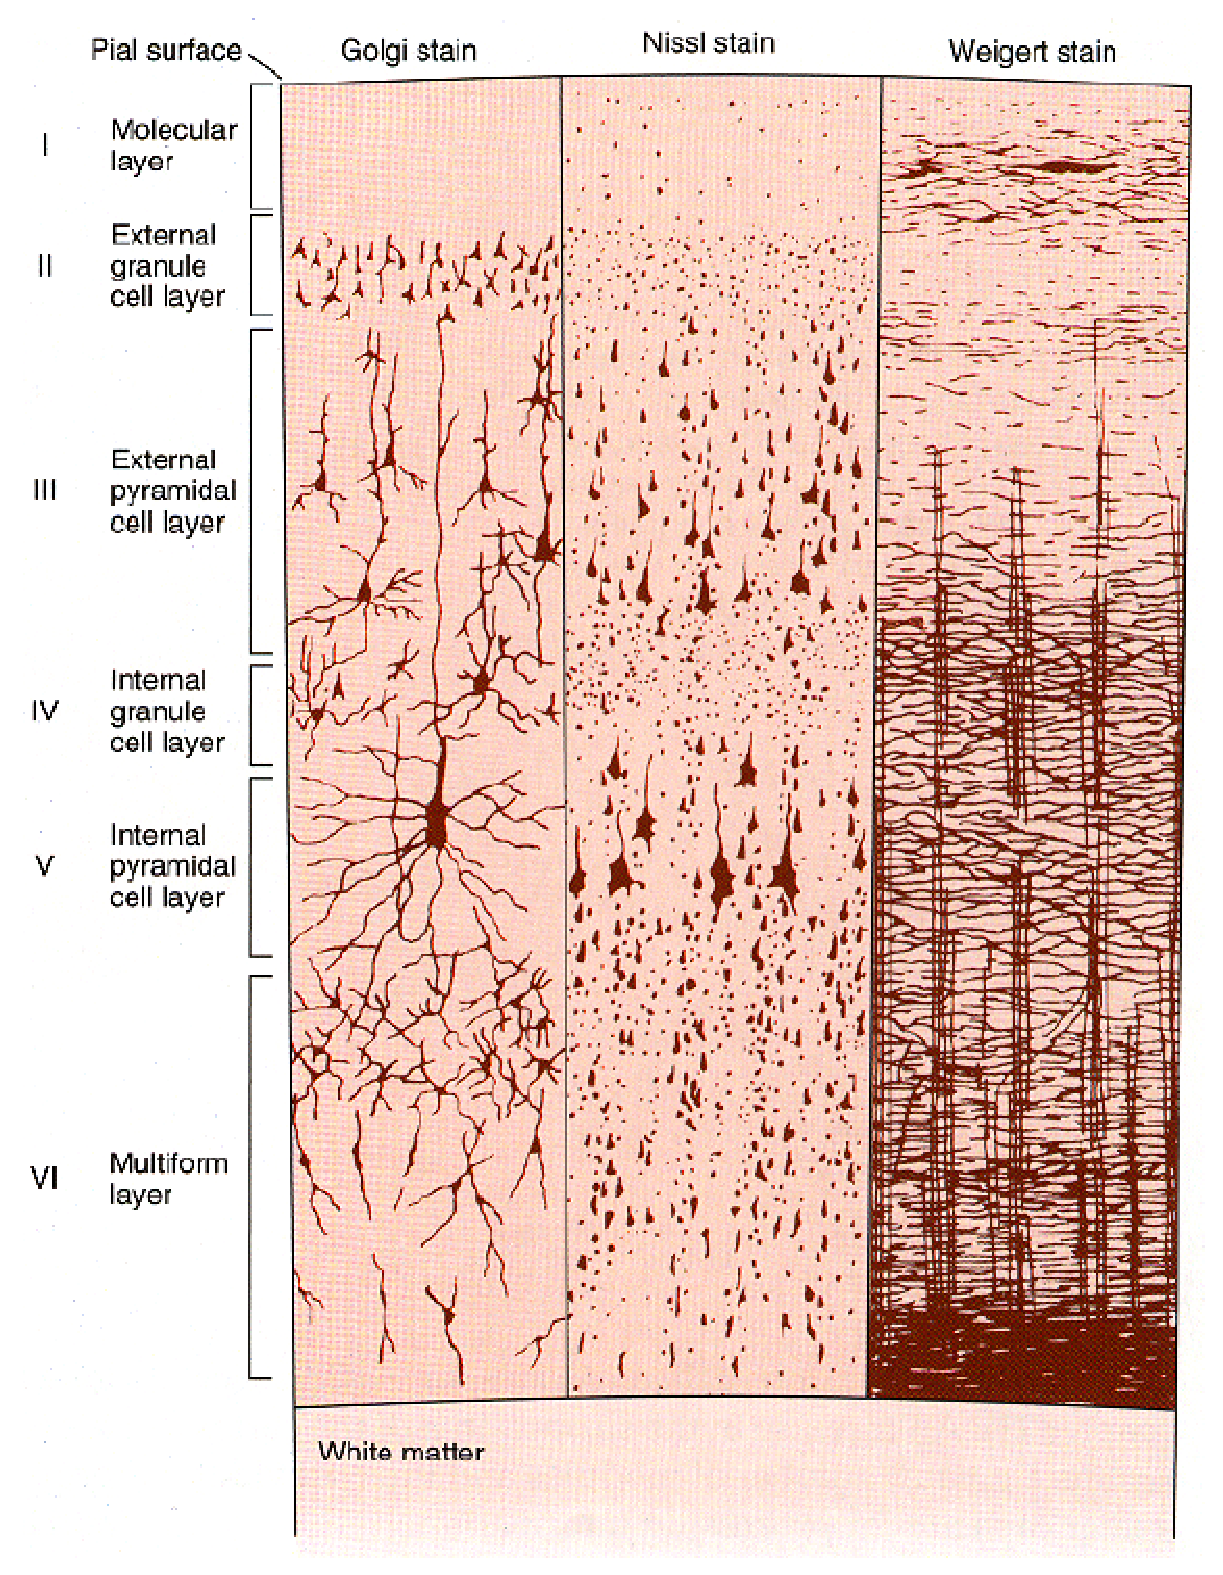
\includegraphics[height=12cm,
    angle=0]{./images/laminal_cerebrum.eps}}
  \caption{Different neural elements are shown in the different layers in neocortex (total
  2-4 mm thick) are revealed by different staining methods: Golgi stain
  (for whole neurons), Nissl stain (mark the ER - soma), Weigert stain (myelin
  stain - axons)
  %(A) neuronal cells + dendrites, (B)
   % proximal dendrites, (C) patterns of axonal distribution
    }
 % \caption{The three drawing of laminal structures of cerebrum by Cajal
 %   (father of neuroscience)}
\label{fig:laminal}
\end{figure}

%Functionally, the layers of the cerebral cortex can be divided into three
% parts.
\begin{enumerate}
  \item {\bf Supragranular layer}: consists of layer I to III
  
  It is highly developed in humans and permits communication between one portion
  of the cortex and other regions. This is the primary origin and terminal of
  intra-cortical connections as either
  \begin{itemize}
    \item associational (i.e., with other areas of the same hemisphere), or
    \item commissural (i.e., connections to the opposite hemisphere, primarily
    through the corpus callosum).
  \end{itemize}
  
  \item {\bf Internal granular layer}: layer IV (Sect.\ref{sec:layer-IV})
  
  
  \item {\bf Infragranular layer}: layer V and VI
  
  The neurons in these layers receive input from the supragranular cells of
  adjacent columns, although they do not reciprocate; instead, they send their
  signals to extracortical regions. 
  It primarily connects the cerebral cortex with subcortical regions
  (Sect.\ref{sec:subcortical-structure}), such as the
  thalamus, and motor and sensory centers. These layers are most
  developed in motor cortical areas.
   
\end{enumerate}

%\subsection{Neuron types}


\subsection{Vertical functional columns: minicolumn, macrocolumn (segregate, hypercolumn), orientation column, barrel
column, ocular dominance column, ontogenetic column}
\label{sec:neocortex_functional-column}
\label{sec:vertical_functional-column}


Review \citep{buxhoeveden2002, rakic2008, jones2010}: 

Horizontal layers and vertical columns are undoubtedly the most dominant
features of cytological organization of the cerebral cortex. However, much works
have been done on horizontal layers (Sect.\ref{sec:neocortex-6-layers}), but not
many in understanding the cortical columns. In this section, we will cover the
later.

The idea that neurons organized into columns of functional similar neurons
started since 1957 by {\bf Mountcastle} as he found that neurons in the
sensory area in the cat organized vertically (or radially in the convoluted
cerebrum) and he estimated unitary column should be about 0.5 mm in diameter. 

{\bf Definition}: ``a (radial cortical) {\bf
functional column} is a segment of neocortex extending through the entire
thickness of the neocortex, occupying the lateral areas of about a few tens of a
millimeter in diameter'', Fig.\ref{fig:cortical-layer_rodent}. However, this
organization is not uniform across the neocortex.
\textcolor{red}{The human cortex is estimated to contain as many as two million
columns each
 having between 50,000 and 100,000 neurons.}
 
In 1972, Rakic and colleagues provided evidence for the embryological origin of
vertical units. Subsequent research by many others has shown that the cortical
columns consist of an array of iterative neuronal groups (also called {\bf
modules}) that extend radially across cellular layers VI to II with layer I at
the top. Currently, there are different terms refering to this modular
structure.


\begin{enumerate}
  \item The {\bf minicolumn} (sometimes referred to as the microcolumn) of
  0.5mm in diameter, with its 80-100 neurones, is the smallest level of vertical
  organization in the cortex.
However, as pointed out by \citep{house2008, rakic2008}, this number is not
applied to all areas in the neocortex as the density of neurons in the neocortex
varies as much as three times even among the highly related primate species.

The minicolumn, and columnar organization in general, is a perspective, a way of
classifying and organizing the cortex.

\item  The {\bf macrocolumn} is a larger unit that consists of many minicolumns,
estimated by some to contain between 60 and 80.

\begin{itemize}
  \item The {\bf segregate} is a specific form of macrocolumn in the somatosensory cortex.

  \item The {\bf hypercolumn} is a form of macrocolumn specific to the visual
  cortex.
\end{itemize}


  \item {\bf orientation column}
  
  \item {\bf barrel column}:
  
  \item {\bf ocular dominance column}
  
  \item {\bf ontogenetic column} (embryonic column):
\citep{rakic2008} coined the term '{\bf ontogenetic column}' in designating the
cohorts of cortical neurons that originate, over time, from a single neuronal
progenitor. 

The relationship between ontogenetic and various functional columns has not been
adequately investigated. However, it's clearly that any functional column in the
adult cerebral cortex must consist of several ontogenetic columns (polyclones),
depending on their function; and that neurons from different clones intermix
with the adjacent columns as they migrate across the intermediate zone
  
\end{enumerate}


However, their is no rigid border for a functional column; it appears that the
structure of functional columns are dynamic, i.e. neurons in a functional column
can ``re-wire'' their lateral connection in response to modulatory control
signals so that these neurons can be a part of many different functional columns
(Chap.\ref{chap:brain_circuitry}).

\begin{figure}[htb]
  \centerline{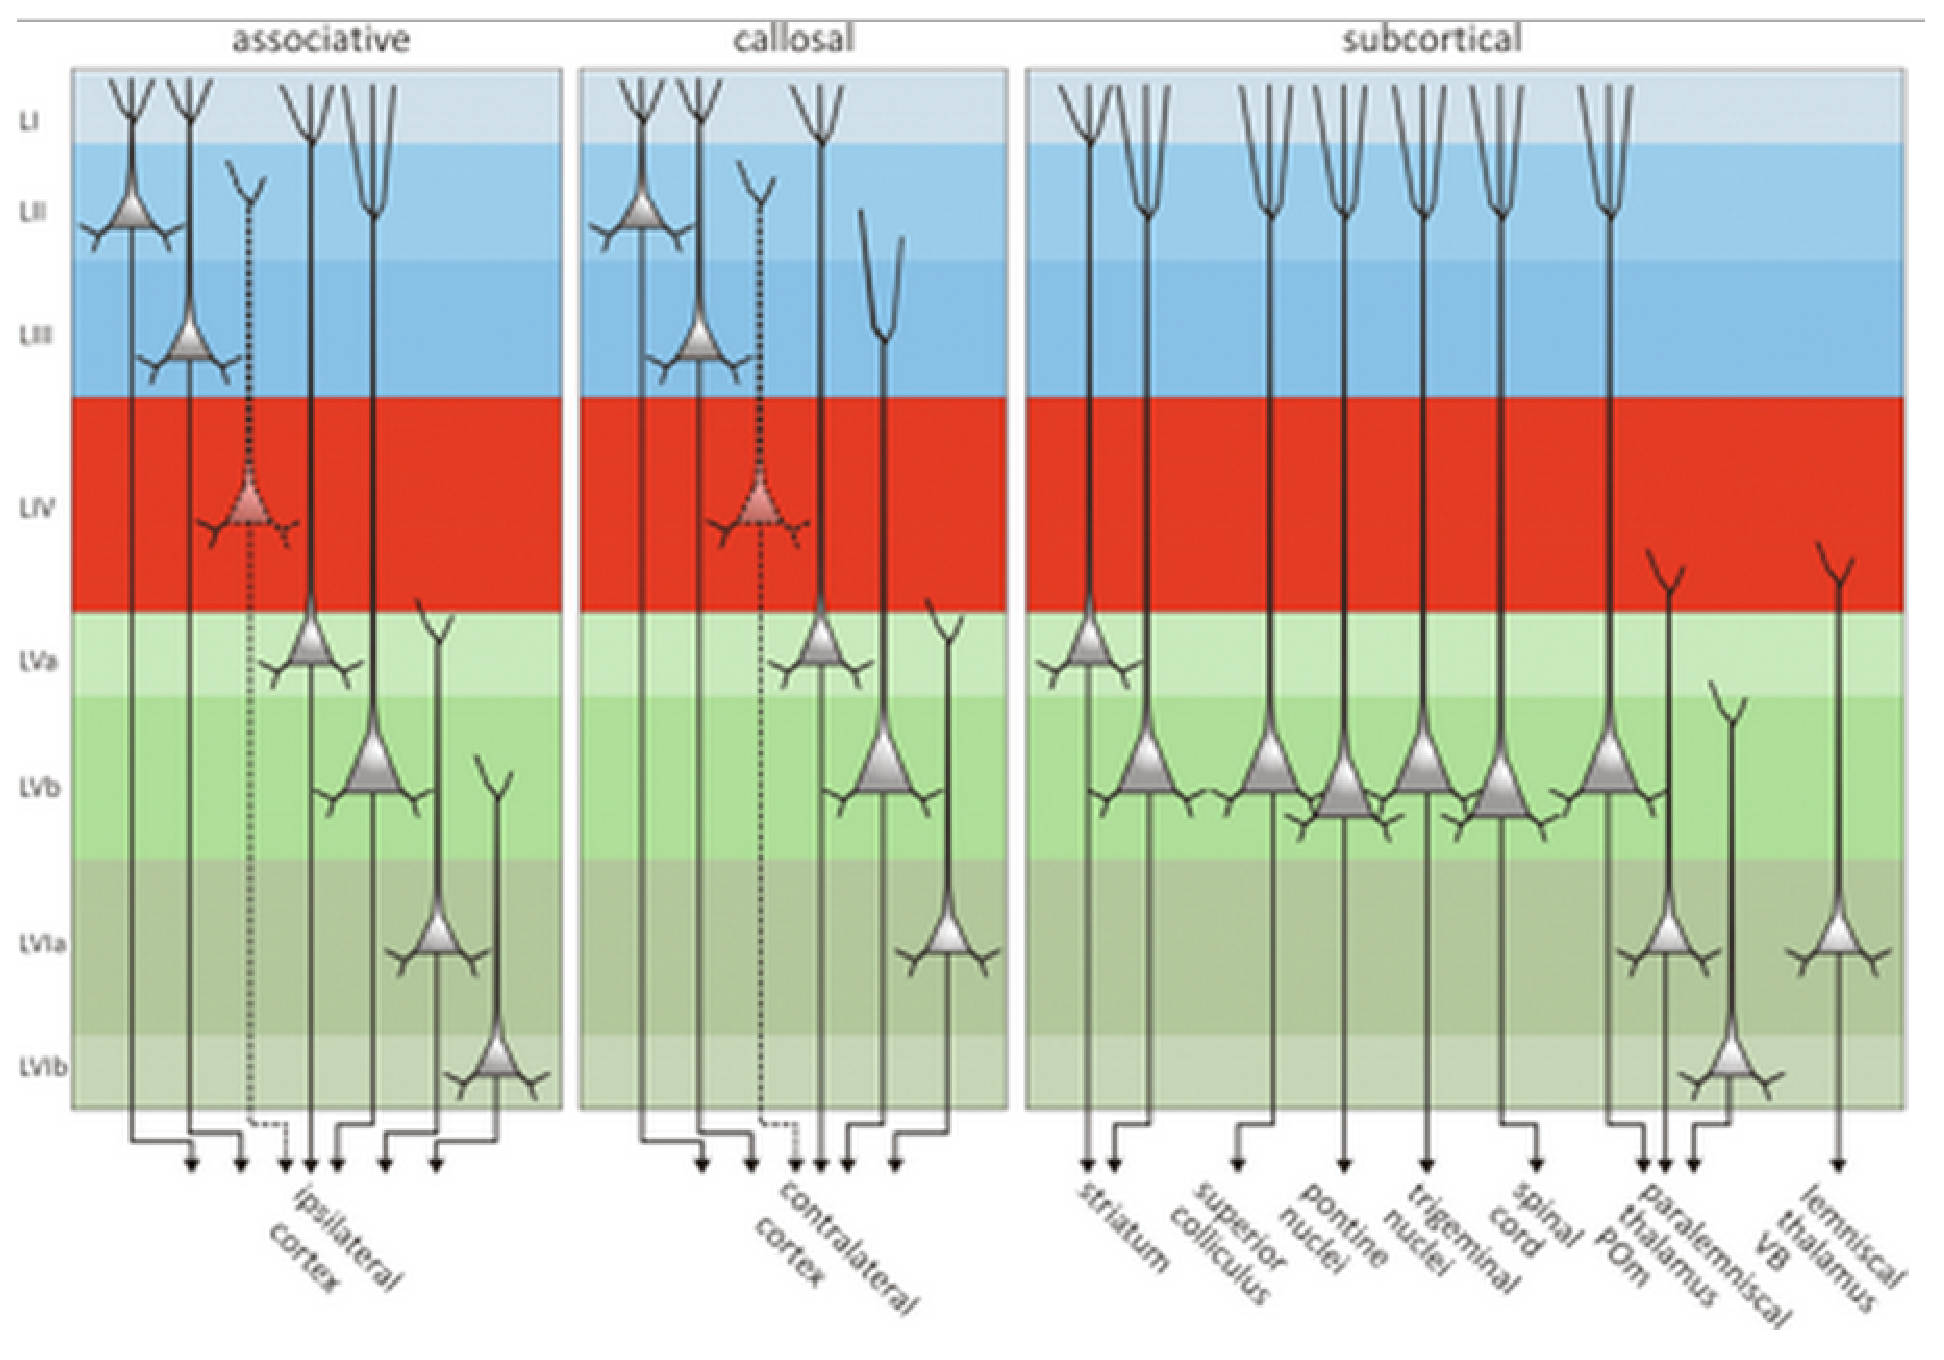
\includegraphics[height=6cm]{./images/cortical-layer_rodent.eps}}
  \caption{Neuron projections in neocortex}\label{fig:cortical-layer_rodent}
\end{figure}




\subsection{Ocular dominance column}
\label{sec:ocular-dominance-column}

Ocular dominance column are neurons in the visual cortex
(Sect.\ref{sec:visual-cortex}) that respond preferentially to input from one eye
or the other; and are laid out in a striped pattern across the surface of
striate cortex (V1). The columns span multiple cortical layers -
Sect.\ref{sec:V1-region}.



\subsection{2 main areas: association cortex + primary cortex}
\label{sec:association-cortex}

Association cortex is the cerebral cortex outside the primary areas,
Fig.\ref{fig:primary-cortex_association-cortex}.

\begin{figure}[htb]
\centerline{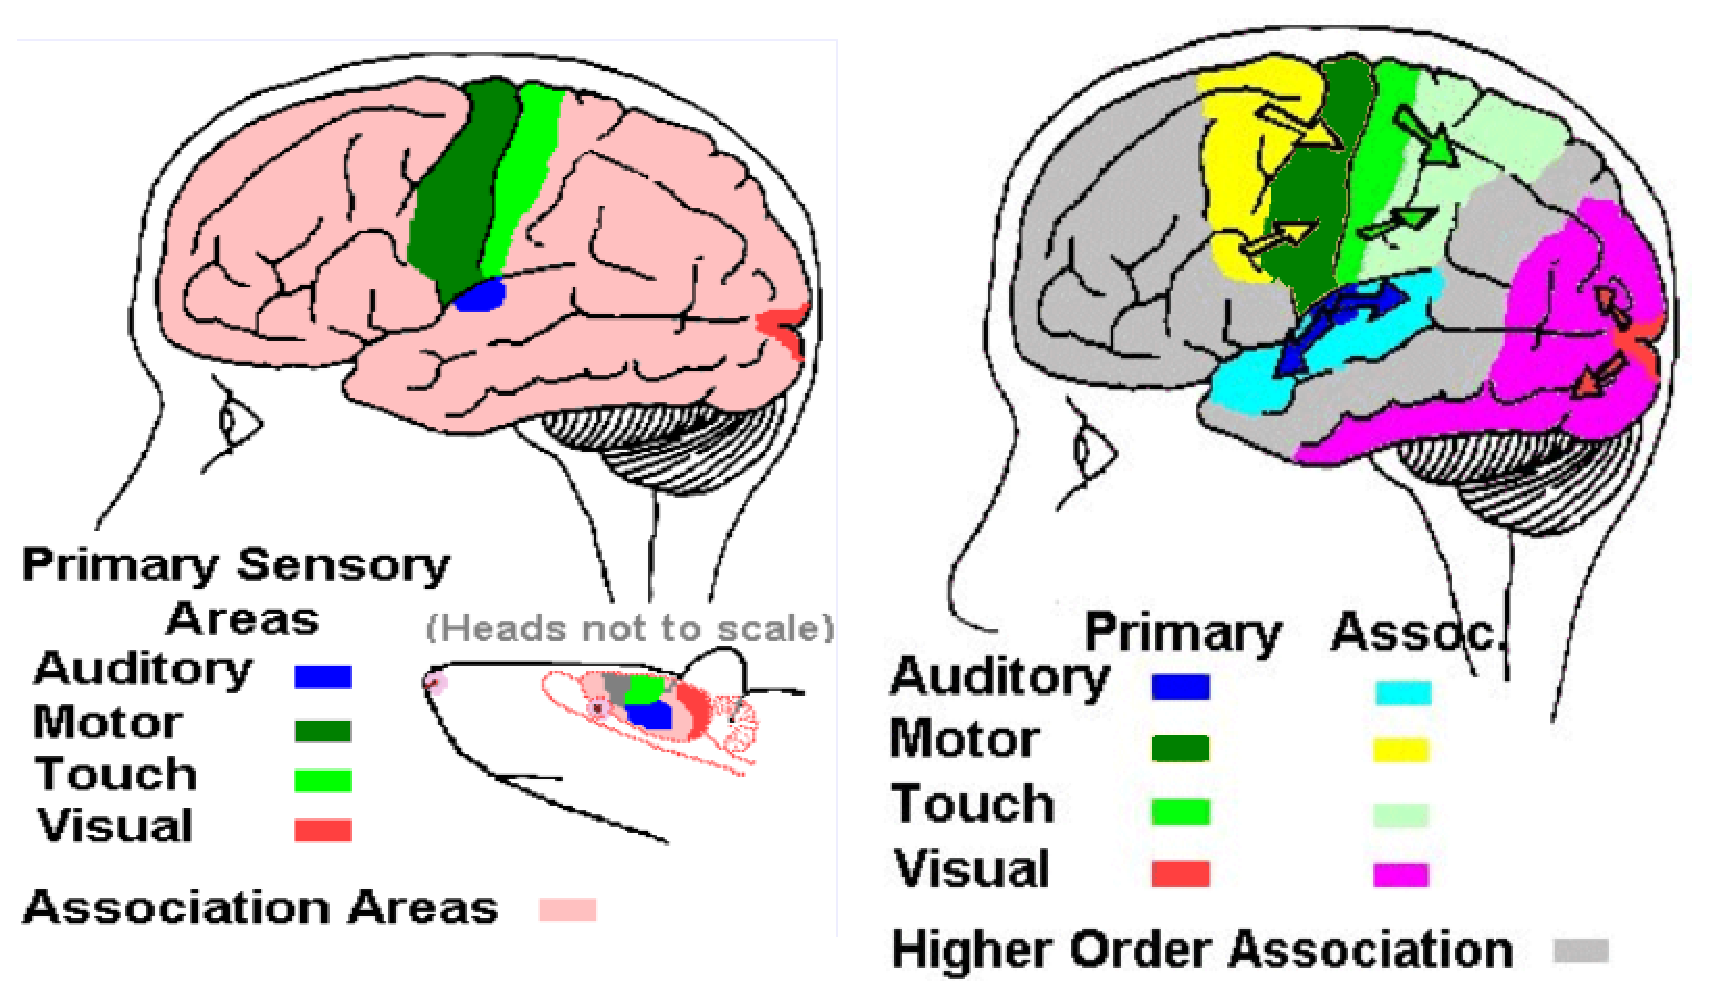
\includegraphics[height=4cm]{./images/primary-cortex_association-cortex.eps}}
\caption{There are 4 different regions of the Primary Cortex; and for each
region there is an association cortex linked to it
}\label{fig:primary-cortex_association-cortex}
%http://www.indiana.edu/~p1013447/dictionary/assn_cor.htm
\end{figure} 

A major part of the association cortex is for higher order association.
Higher order association cortex carries out complex mental processes not
associated with any particular sense.
The higher order association areas combine information from several sensory
association areas. Each sensory and motor association areas sends signals to
higher order association areas, which combine this information to form the basis
of the highest mental processes.
These highest mental processes, like language, thinking, and planning, do not
depend on specific sensory information.
For example, language can use vision (reading, sign language) and touch (Braille
for the blind), as well as hearing.

\subsection{Primary cortex}
\label{sec:primary-cortex}


There are 4 different regions of primary cortex:
\begin{enumerate}
  \item auditory primary cortex - Sect.\ref{sec:auditory-cortex}
  \item motor primary cortex - Sect.\ref{sec:motor-cortex}
  \item touch (somatosensory) primary cortex - Sect.\ref{sec:somatosensory-cortex}
  \item visual primary cortex - Sect.\ref{sec:visual-cortex}
\end{enumerate}

\subsection{* Visual cortex}
\label{sec:visual-cortex}

David Hunter Hubel, Roger Wolcott Sperry, and Torsten Wiesel received Nobel
prize in 1981 for their study on visual cortex:
\begin{enumerate}
  \item Hubel and Wiesel discovered orientation selectivity and columnar
  organization in visual cortex: {\bf ocular dominance column}
  (Sect.\ref{sec:ocular-dominance-column})
\ref{sec:vertical_functional-column}
A microelectrode is inserted into the primary visual cortex of an anesthetized
cat; and the cat is given pictures of patterns of light and dark, and they
found: (1) {\bf simple cells} (Sect.\ref{sec:simple-cell}) - neurons responded
to light patterns differently, i.e. some neurons fired rapidly when presented
with lines at one angle and some other responded best to another angle; (2) {\bf
complex cells}
 
   
  \item 
\end{enumerate}


{\bf Visual cortex} comprises Brodmann area 3a, 3b, 1, and 2.

To help understanding the role of visual cortico-striatal connection in
mediating the formation of visuo-motor association, i.e. visual 'habits',
several studies have been done (Sect.\ref{sec:cortico-striatal-loops}).
\begin{verbatim}
visual cortex ---> caudate (striatum) ---> portion of SNr 
                                          (in visual control 
                                          eye movement)
\end{verbatim}

Using anterograde and retrograde tracing techniques, \citep{saint-cyr1990}
studies the connection to the tail and genu of caudate 
\begin{itemize}
  \item (mainly) layer V of the isocortex
  \item (some) layer III and VI of the isocortex
\end{itemize}
connect to the caudate of the striatum

\citep{khibnik2014} found that the primary visual cortex (V1) has strong 
excitatory connections with both direct- and indirect-pathway striatal
projection neurons (SPN)
\begin{itemize}
  \item stimulation of V1 afferents is sufficient to evoke phasic firing in
  SPNs, suggesting early visual processing may play an important role in
  striatal-based behaviors.
  
  81\% is from layer 5 pyramidal cells in primary visual cortex (V1) project to
  the striatum (i.e. dorsomedial striatum (DMS)) of mice, with the predominant
  neurons are intratelencephalic neurons (Sect.\ref{sec:Intratelencephalic-neurons})
  
  19\% is from layer 2/3 pyramidal cells in primary visual cortex (V1) project to
  the striatum (i.e. dorsomedial striatum (DMS)) of mice
  
  On rare occasions, cells in layer 6 were observed, but they constituted a
  negligible percentage of the total number of corticostriatal neurons.
  
  \item 
\end{itemize}

\subsection{* Auditory cortex}
\label{sec:auditory-cortex}

{\bf Auditory cortex} comprises Brodmann area 41, 42 and partially area 22.
It was previously subdivided into primary (A1) and secondary (A2) projection
areas. The modern division of auditory cortex are
\begin{enumerate}
  \item the core (include A1)
  
  \item the belt 
  
  \item the parabelt
\end{enumerate}
Like many areas in the neocortex, the functional properties of the adult primary
auditory cortex (A1) are highly dependent on the sounds encountered early in
life.

The primary auditory cortex receives direct input from the medial geniculate
nucleus of the thalamus (Sect.\ref{sec:thalamus}).
At the auditory cortex, the signals are translated -- transduced -- into
information that scientists call representations. These representations, in
turn, form the informational basis upon which other parts of the brain can make
decisions and issue commands for specific actions, e.g. muscle movement.
However, how the auditory representations are transformed into motor commands is
not known.

Znamenskiy and Zador (2013) showed that even though many neurons in auditory
cortex are "tuned" to low or high frequencies, most do not transmit their
information directly to the striatum.
Instead, a smaller group of neurons in their vicinity, which convey their
'votes' (representing the much larger population of neurons in the auditory
cortex) directly to the striatum \citep{znamenskiy2013}.
\begin{verbatim}
corticocortical connection 
(many cortical neurons ----> smaller grou of cortical neurons ---> striatum
\end{verbatim}

When testing a person listening to temporally regular (periodic) or temporally
irregular (nonperiodic) sequences of tones while performing an intensity
discrimination task, the person can do the task better when listening to
periodic tone sequence, during which there are greater activation in the
putamen; while there are more activation in the auditory cortex for nonperiodic
tone sequence than preiodic sequence. In other words, when there is less
auditory activation in both right and left hemisphere, there are more putamen
activation. It is thus suggested that {\it temporal regularity of sound is
detected by putamen in the striatum} \citep{geiser2012}.

The primary auditory cortex (A1) is subject to the modulation of numerous
neurotransmitters including norepinephrine (NE, Sect.\ref{sec:norepinephrine}),
which has been shown to decrease cellular excitability. \citep{dinh2009}
suggested NE activates $\alpha_1$ AR (Sect.\ref{sec:alpha-adrenergic-receptor}),
PLC, and $\Ca$-independent PKC.


%\subsection{Brain structures: nuclei + layered structure}

\subsection{* Motor cortex}
\label{sec:motor-cortex}


Motor cortex is part of the motor pathway (Sect.\ref{sec:motor-pathway}).
{\bf Motor cortex} column is the region of the cerebral cortex
(Sect.\ref{sec:cerebral_cortex}) involved in the planning, control, and
execution of voluntary movements. 
Motor task directives are initiated from this region.

\begin{mdframed}
One of the most important events in the history of neuroscience is the
discovery, by Fritsch and Hitzig (1870), that electrical stimulation of the
cerebral cortex (Sect.\ref{sec:cerebral_cortex}) produces discrete movement,
i.e. causing muscle contraction (spasms and twitches) in their study. It means
that the \textcolor{red}{nerve cells in the cerebral cortex are excitable.} 

In 1873, David Ferrier published a study of electrical stimulation in
cerebral cortex with more complex movements.
Ferrier later tested a much greater extent of the cortex, and located motor
centers in several cortical regions, e.g.
frontal eye field (area 8 - eye movement area) (review: \citep{taylor2003}).

\end{mdframed}


\begin{figure}[hbt]
  \centerline{
  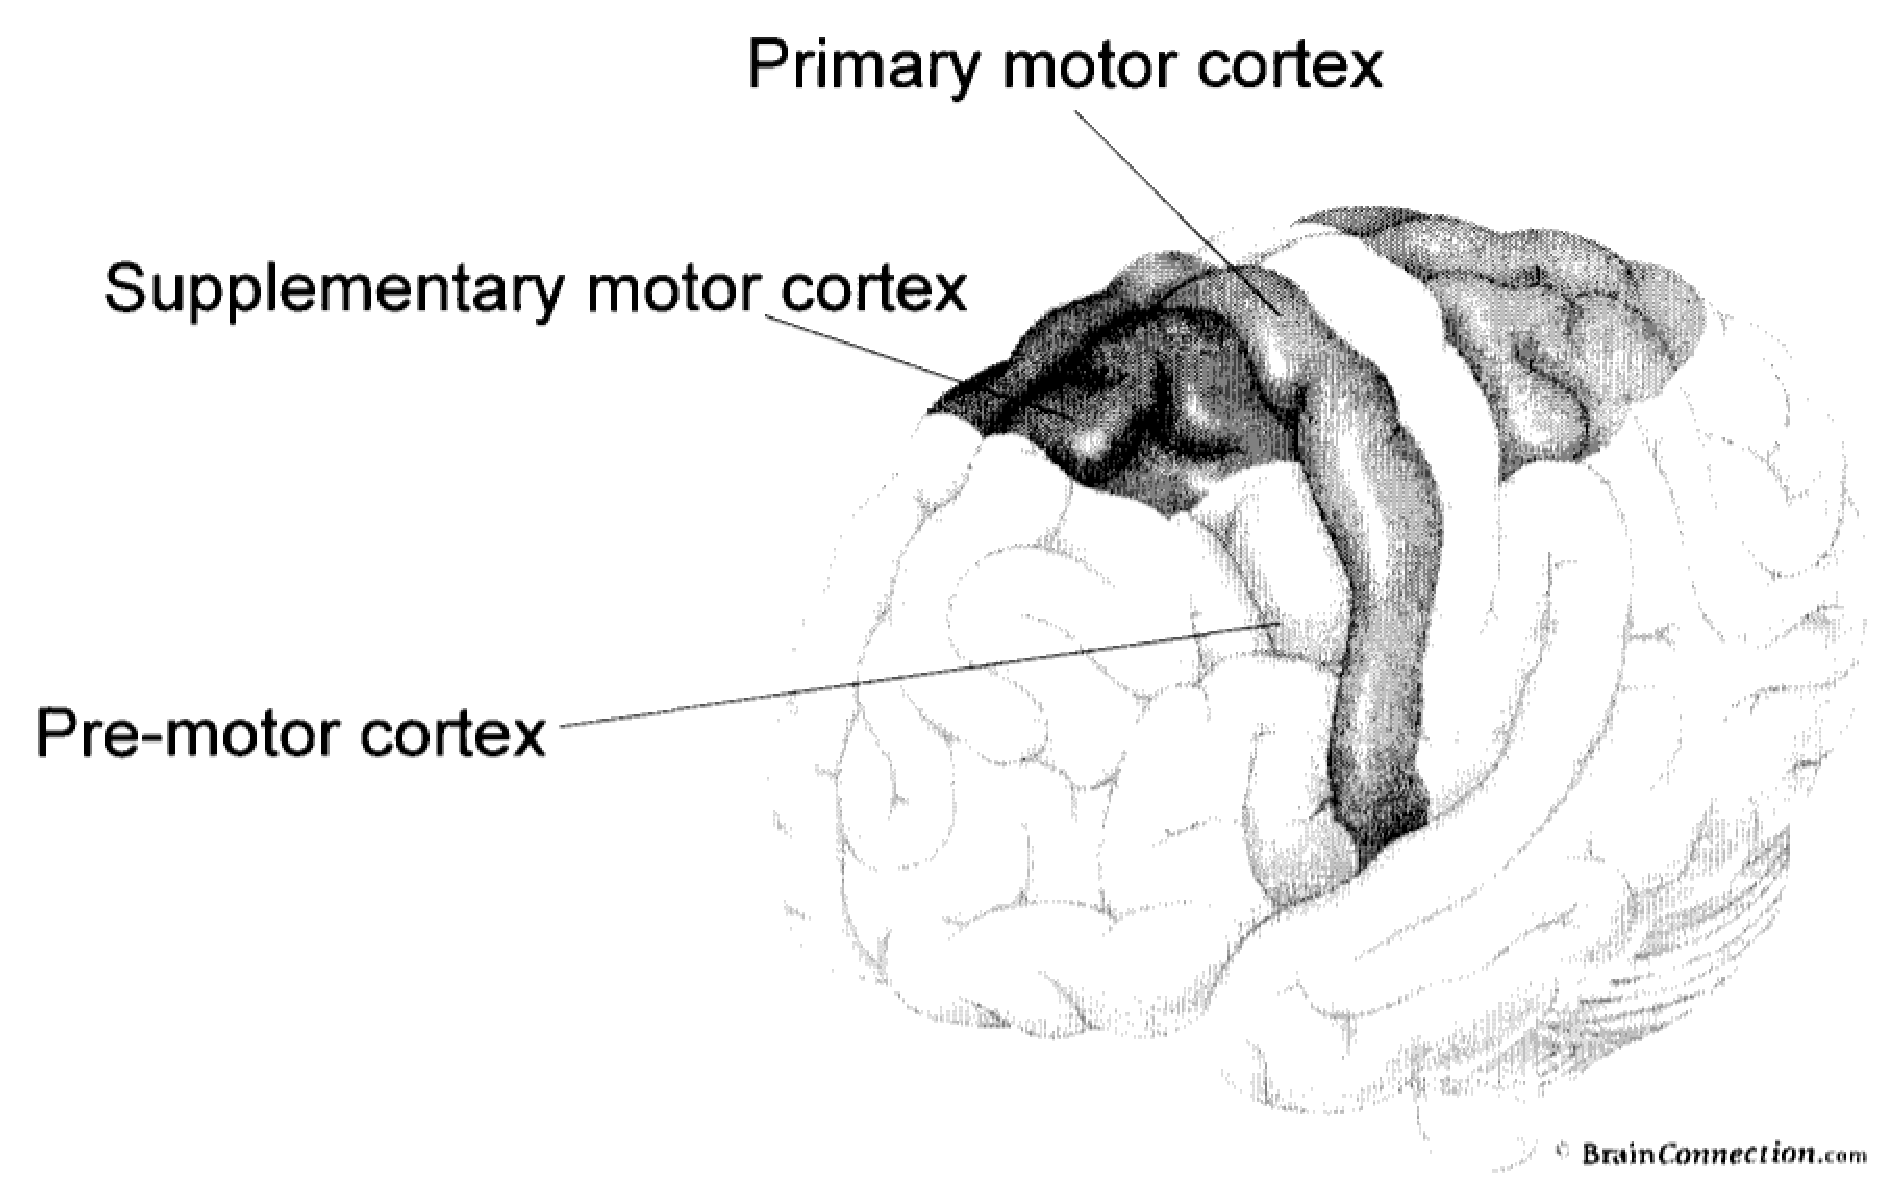
\includegraphics[height=4cm,
    angle=0]{./images/motor-cortex.eps}}
  \centerline{
  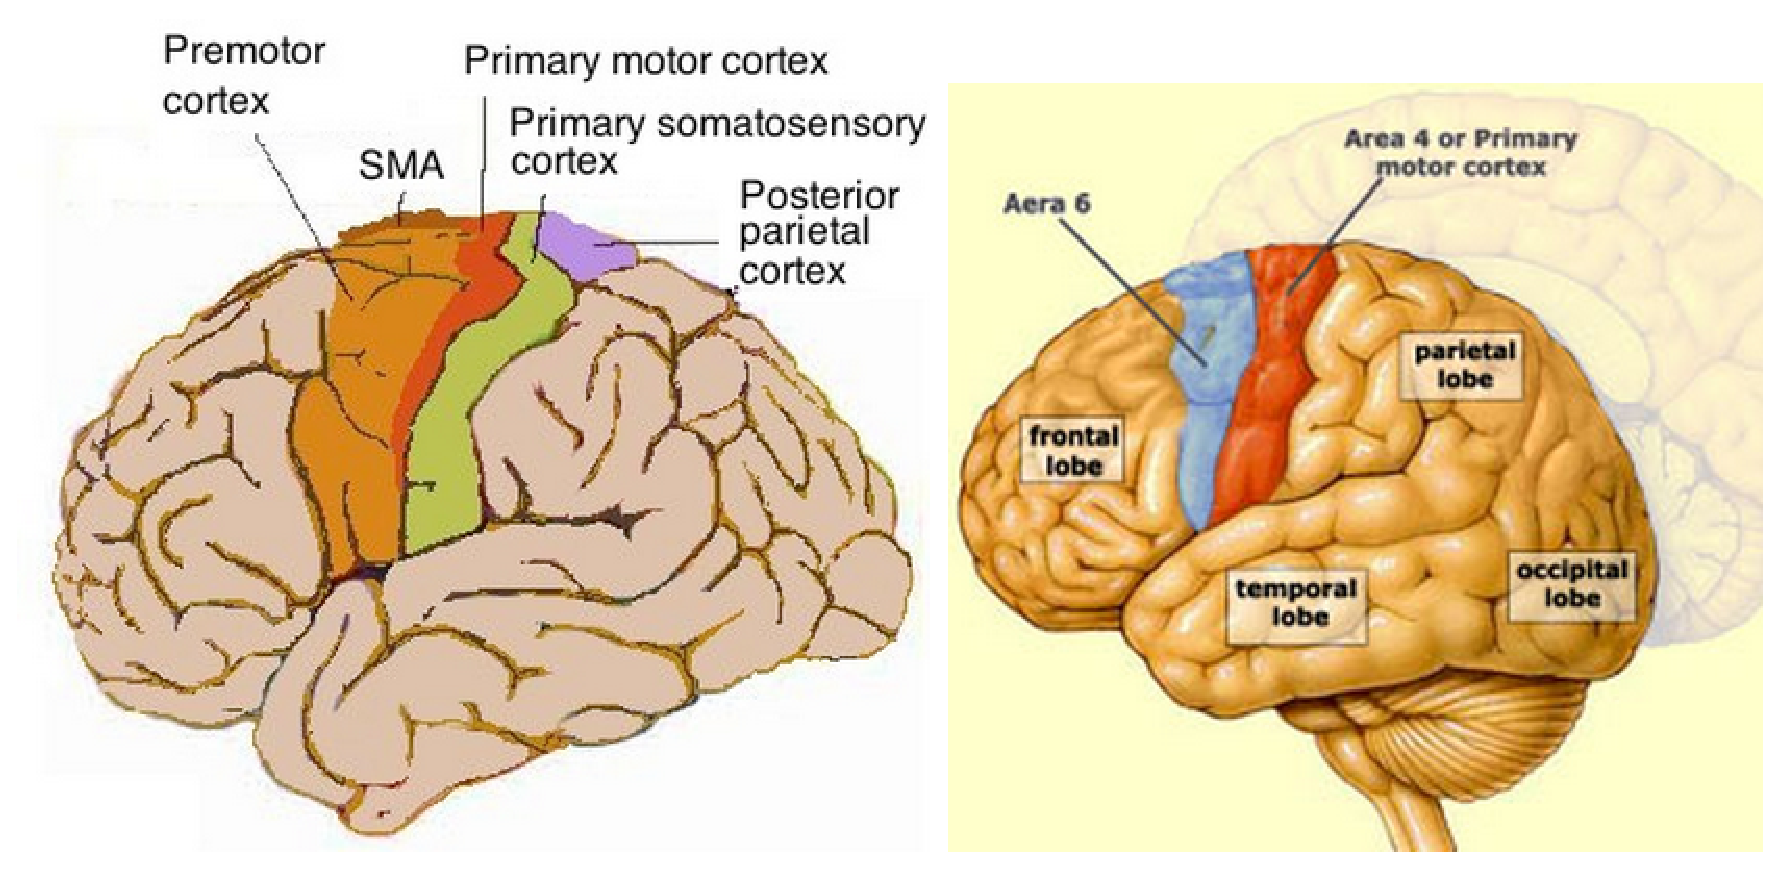
\includegraphics[height=4cm,
    angle=0]{./images/motor_cortex.eps}}
\caption{Human motor cortex: premotor cortex, SMA, primary motor cortex,
primary somatosensory cortex, posterior parietal cortex}
\label{fig:motor_cortex}
\end{figure}

Motor cortex can be divided into 3 areas, Fig.\ref{fig:motor_cortex} and
Fig.\ref{fig:Brodmann_area} with different types of motor neurons
(Sect.\ref{sec:motor-neuron}): (SchieberandBaker,2003).
\begin{enumerate}
  \item {\bf primary motor cortex} (M1, brain area 4):
  Sect.\ref{sec:M1-region}.

  
   \item {\bf premotor cortex} (premotor area (PMA), part of brain area 6):
   Sect.\ref{sec:premotor-cortex}
  
  \item {\bf supplementary motor cortex} (supplementary motor area (SMA), part
  of brain area 6): Sect.\ref{sec:SMA}
\end{enumerate}


There are so many different motor movements, corresponding to different parts of
the body. Dr. Penfield developed the map called {\bf motor homonculus} (Latin:
homonculus = little man) that map each region of the motor cortex to the
movement of the associated body part, Fig.\ref{fig:motor_homonculus}.
The most striking aspect of this map is that the areas of the brain assigned to
various body parts on the cortex are proportional not to the size of the body
parts, but rather to the  complexity of the movements that the body parts can
perform.

\begin{figure}[hbt]
  \centerline{
  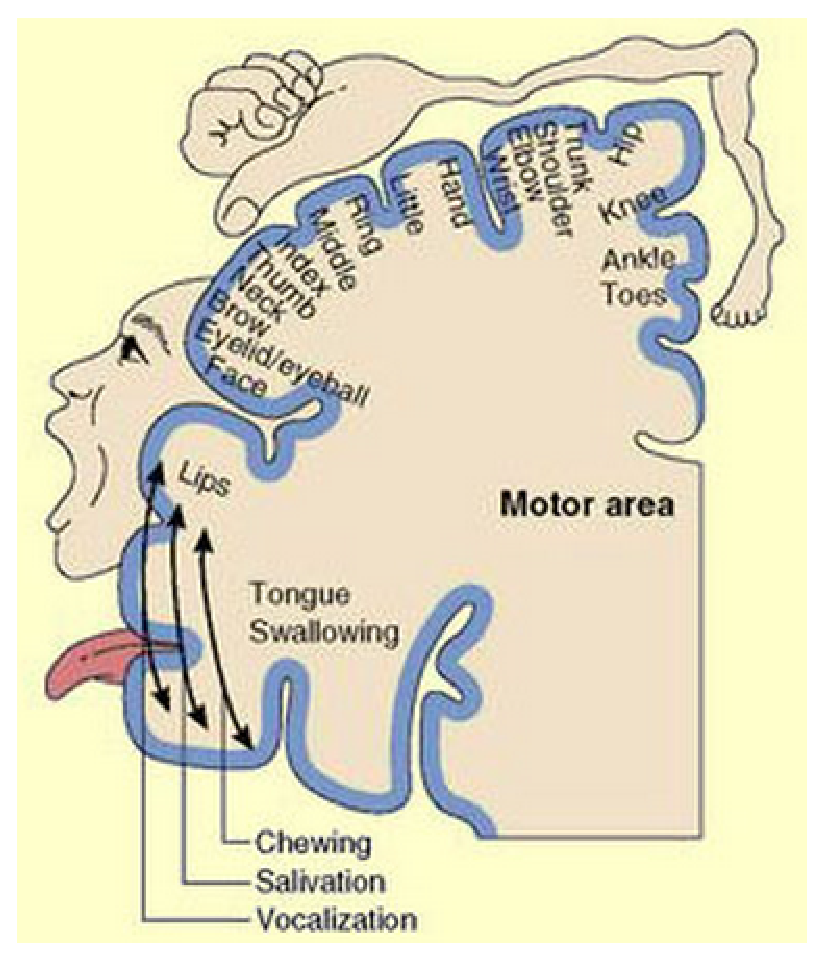
\includegraphics[height=5cm,
    angle=0]{./images/motor_homonculus.eps}}
\caption{The motor homonculus: the map mapping motor cortex to different motor
movement}
% http://thebrain.mcgill.ca/flash/i/i_06/i_06_cr/i_06_cr_mou/i_06_cr_mou.html
\label{fig:motor_homonculus}
\end{figure}


\subsection{-- Premotor cortex (brain area 6)}
\label{sec:premotor-cortex}

NOTE: brain area 6 is divided into 2 parts: premotor cortex - the
lateral portion, and supplementary motor area (SMA).
   
Premotor cortex is  responsible for some aspects of motor control,
   e.g.  sensory guidance of movement, activation of proximal muscles as well as trunk muscles that orient
  the body (Berkowitz \& Ansari, 2008).
  \begin{enumerate}
    \item premotor cortex dorsal rostral (PMdr)
    \item cingulate motor area caudal (CGc)
    \item cingulate motor area rostral (CGr)
    \item premotor cortex ventral caudal (PMvc)
    \item premotor cortex ventral rostral (MPvr)
    \item pre-supplementary motor area (Pre-SMA)
  \end{enumerate}

\subsection{-- SMA (supplementary motor cortex - brain area 6)}
\label{sec:SMA}

SMA (part of brain area 6) is involved in planning complex movements and in
co-ordinating movements involving both hands (Bernard
et al., 2002; Wiese et al., 2004)

\subsection{* Prefrontal cortex (PFC)}
\label{sec:prefrontal-cortex}

The prefrontal cortex (PFC) is the front part of the frontal lobe
(Sect.\ref{sec:frontal-lobe}). 

There are different ways to subdivide the prefrontal cortex starting from
Brodmann areas (Sect.\ref{sec:Brodmann_area}), Fig.\ref{fig:Brodmann_area-PFC}. 
 
\begin{figure}[hbt]
  \centerline{
  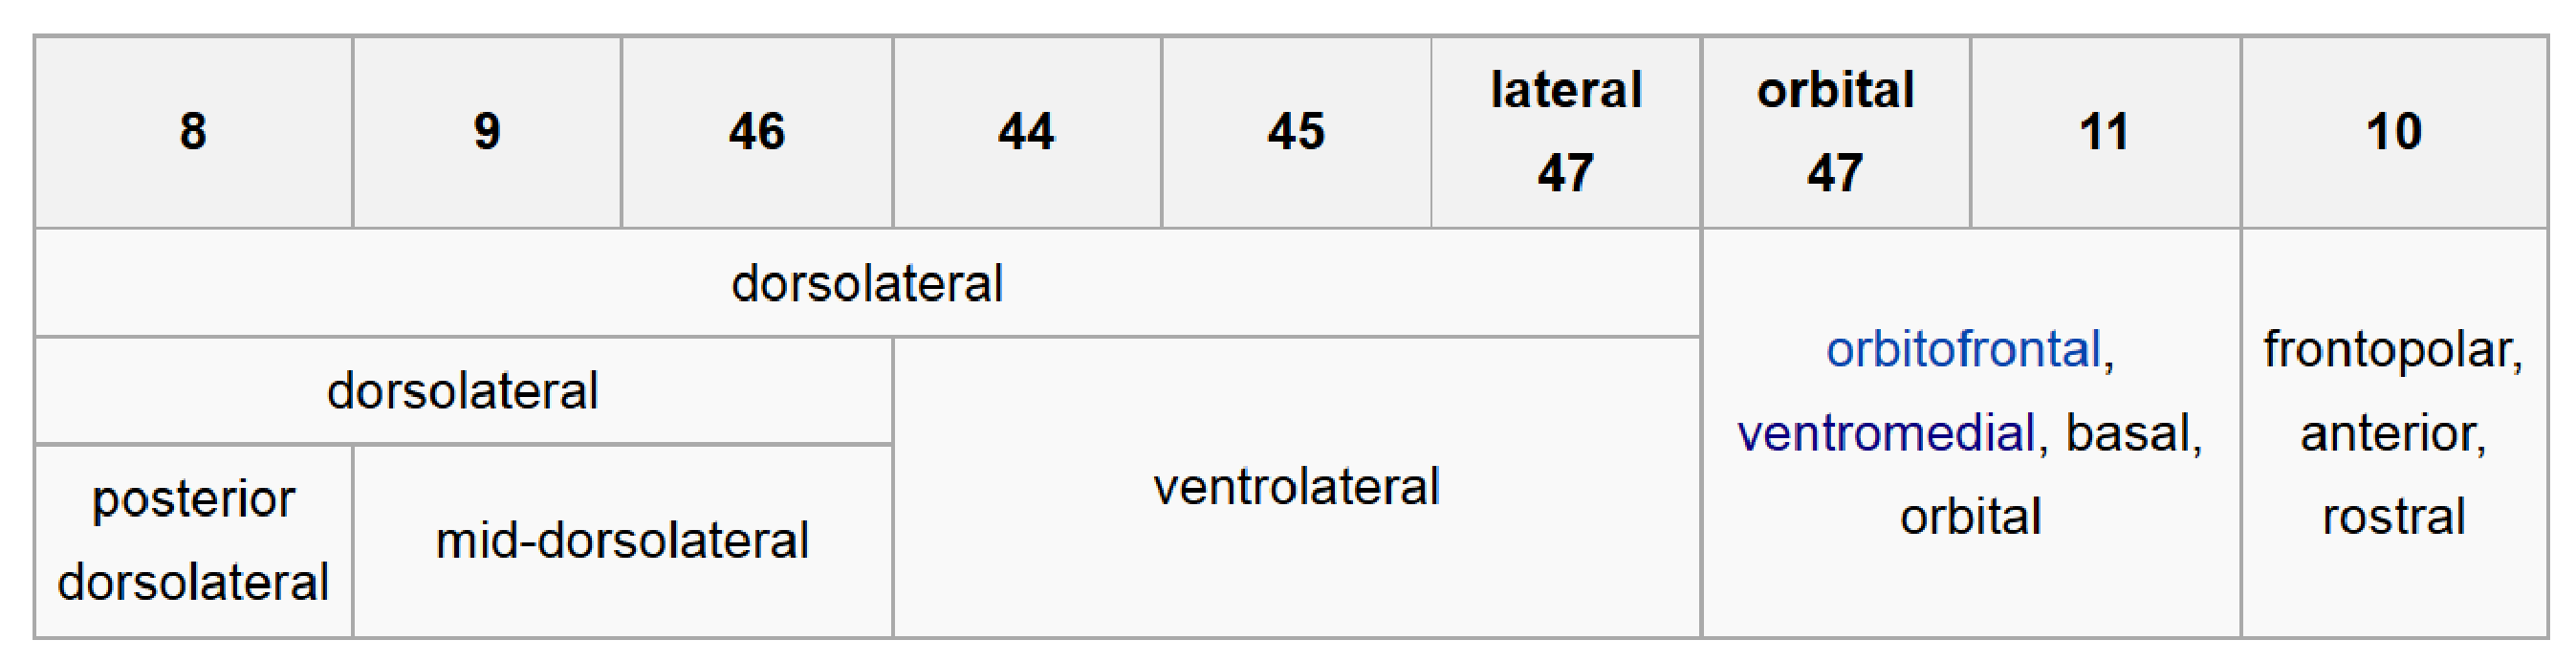
\includegraphics[height=3cm,
    angle=0]{./images/Brodmann_area-PFC.eps}}
\caption{NOTE: Note that the term "dorsolateral" has been used to denote areas
8, 9, and 46 as well as areas 8, 9, 44, 45, 46, and lateral 47. Several terms
are given to areas 47, 11 and 10}
\label{fig:Brodmann_area-PFC}
\end{figure}
 
 
The prefrontal cortex is divided into 3 parts:
\begin{enumerate}
  \item dorsolateral: There are two uses of this terms
  \begin{itemize}
    \item Case 1: Brodmann areas: 8, 9, 46
    \item Case 2: Brodmann areas: 8, 9, 46, 44, 45, lateral 47
  \end{itemize}
  
  \item Case 1: 3 other regions: ventrolateral, orbitofrontal (ventromedial,
  basal, orbital), and frontopolar (anterior, rostral)
  
  \item Case 2: orbitofrontal (ventromedial,  basal, orbital),
  and frontopolar (anterior, rostral)
\end{enumerate}

\subsection{** dorsolateral prefrontal cortex (dLPFC)}
\label{sec:dLPFC}

dlPFC is not an anatomical structure, but is a 
functional one, as it can be composed of different Brodmann area in different
species.
\begin{itemize}
  \item Human: Between Brodmann's area (BA) 9 and area 46: dorsolateral
  prefrontal cortex (dLPFC)

  \item Monkey: in Walker's area 46: dorsolateral prefrontal cortex (dLPFC)
\end{itemize}
Other sources consider that dlPFC is attributed anatomically to BA 9 and 46
and BA 8, 9 and 10.

dLPFC plays a dominant role in executive function or goal-directed behavior, and
mediates both learning the 'rule of the game', and dynamically updating those
rules as contingencies are altered.
To study dLPFC, different tests have been used
\begin{itemize}
  \item A-not-B task (or delayed
  matching to sample task) (Sect.\ref{sec:delayed-matching-to-sample-task}):
  \textcolor{red}{This is the task most strongly linked dLPFC}.
  
  The behavioral task that is most strongly linked to dlPFC is the combined
  A-not-B/delayed response task, in which the subject has to find a hidden
  object after a certain delay. 
  This task requires holding the information in mind (working memory) which is
  believed to be one of the functions of dLPFC.
  
  \item Delayed response task (Sect.\ref{sec:delayed-response-task})
  
  \item Object retrieval task 
\end{itemize} 

\subsection{** ventromedial prefrontal cortex (vmPFC), orbitofrontal}
\label{sec:ventromedial prefrontal cortex}
\label{sec:vmPFC}

The ventromedial prefrontal cortex (vmPFC) is a part of the prefrontal cortex in
the mammalian brain  (Sect.\ref{sec:prefrontal-cortex}). It is implicated in the
processing of risk and fear. It also plays a role in the inhibition of emotional
responses, and in the process of decision making.


\subsection{** Frontopolar prefrontal cortex}
\label{sec:frontopolar-prefrontal-cortex}
 
area 10: frontopolar prefrontal cortex


\subsection{Basal forebrain}
\label{sec:basal-forebrain}

The basal forebrain is a collection of structures 
\begin{enumerate}
  \item NAc
  \item Nucleus Basalis - Sect.\ref{sec:nucleus-basalis}
  \item  diagonal band of Broca
  \item  substantia innominata - Sect.\ref{sec:substantia-innominata}
  \item medial septal nuclei.
\end{enumerate}
located to the front of and below the striatum (Sect.\ref{sec:striatum}),
Fig.\ref{fig:basal-forebrain}.
These structures are important in the production of acetylcholine, i.e. the
major cholinergic output of the brain (Sect.\ref{sec:cholinergic_neurons}),
which is then distributed widely throughout the brain.

The basal forebrain and adjacent areas are a focus for sleep research.
It is believed that nitric oxide production in the basal forebrain is both
necessary and sufficient to produce sleep. 

\begin{figure}[hbt]
  \centerline{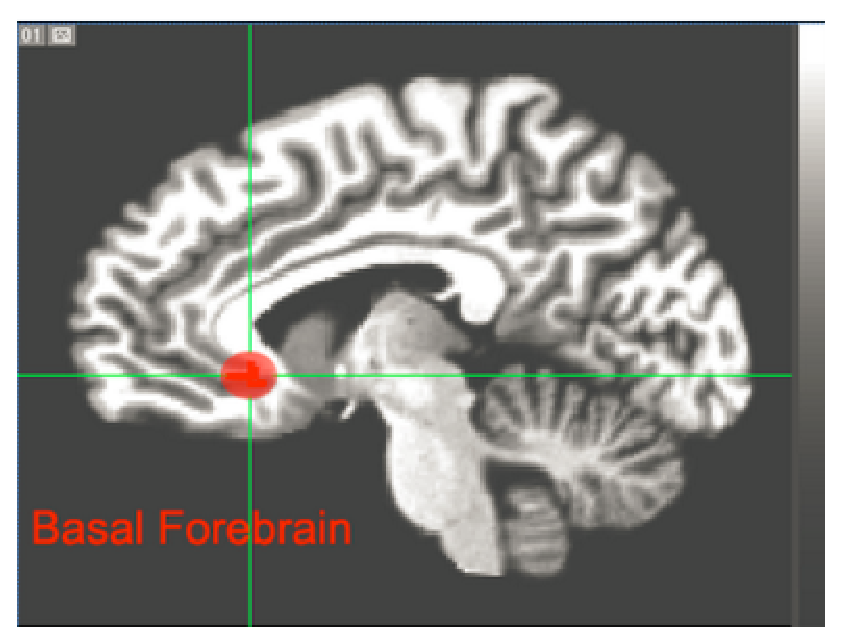
\includegraphics[height=3cm,
    angle=0]{./images/basal-forebrain.eps}}
  \caption{Basal forebrain: located to the front and below the striatm
  (caudate + putament)}
  \label{fig:basal-forebrain}
\end{figure}

\subsection{-- substantia innominata of Meynert}
\label{sec:substantia-innominata}

The substantia innominata (literally "unnamed substance") of Meynert is a
stratum in the human brain, consisting partly of gray and white substance.
It is part of the basal forebrain (Sect.\ref{sec:basal-forebrain}) and the major
neurons are the nucleus basalis of Meynert (Sect.\ref{sec:nucleus-basalis}).

It has 3 layers:
\begin{itemize}
  \item superior layer (ansa lentiformis)
  \item middle layer (nerve cells + nerve fibers)
  \item inferior layer (form the main part of the inferior stalk of the
  thalamus)
\end{itemize}
% The nerve cells in this area is called Nucleus basalis of Meynert
% (Sect.\ref{sec:nucleus-basalis}).

\subsection{---- Nucleus basalis of Meynert}
\label{sec:nucleus-basalis}

\begin{mdframed}
Theodor Hermann Meynert was a German-Austrian neuropathologist and anatomist in
19th century (1833-1892). He is often considered to be the founder of cerebral
cortex cytoarchitectonics. He has several anatomical structures named after him,
e.g. Meynert cells - Sect.\ref{sec:Meynert-cell}, nucleus basalis of Meynert.
\end{mdframed}

{\bf Nucleus basalis of Meynert} (NBM) is the nucleus in the substantia
innominata of the basal forebrain (Sect.\ref{sec:substantia-innominata}),
located in the deep gray and white matter that lies anterior to the thalamus and
basal ganglia, Fig.\ref{fig:nucleus-basalis-Meynert}.
\begin{itemize}
  \item  The human nucleus basalis extends from the level of the olfactory
  tubercle to that of the posterior amygdala, spanning a distance of 13-14mm in
  the anteroposterior axis and attaining a mediolateral width of 18mm within the
  substantia innominata (subcommissural gray).
  
It contains approximately 200000 neurons in each hemisphere.

  \item   
  
\end{itemize}
The primate nucleus basalis projects to the entire cerebral cortex, it receives
major cortical projections from 
\begin{itemize}
  \item  The hippocampus and cerebral neocortex receive massive cholinergic
  projections from the basal forebrain.
\end{itemize}


\url{http://www.sciencedirect.com/topics/page/Nucleus_basalis_of_Meynert}


The NBM contains 
\begin{enumerate}
  \item the cell bodies of neurons (Sect.\ref{sec:cholinergic_neurons})
that project cholinergic axons to the cerebral cortex.

  \item  also contains a complex mosaic of noncholinergic
  neurons that are nicotinamide adenine dinucleotide phosphate diaphorase
  (NADPHd)-positive, $\gamma$-aminobutyric acid (GABA)ergic, peptidergic, or
  tyrosine hydroxylase-positive
\end{enumerate}

\begin{figure}[hbt]
  \centerline{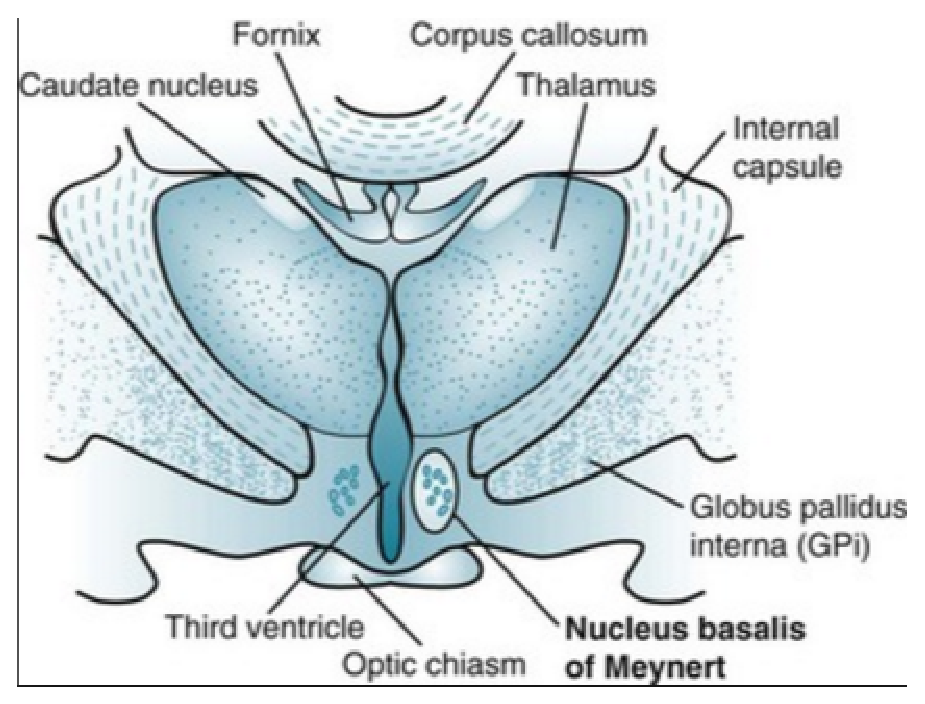
\includegraphics[height=3cm,
    angle=0]{./images/nucleus-basalis-Meynert.eps}}
  \caption{The nucleus basalis of Meynert}
  \label{fig:nucleus-basalis-Meynert}
\end{figure}

% comprised by a group of
% cholinergic neurons in the substantia innominata of the basal forebrain
% (Sect.\ref{sec:substantia-innominata}). They project into the neocortex, and are
% rich in acetylcholine and choline acetyltransferase
% (Sect.\ref{sec:cholinergic_neurons}).

Based on its location, connectivity, and cellular morphology, the nucleus
basalis has been conceptualized as a site of confluence for the limbic system
and the ascending reticular activating system.

In Parkinson' and Alzheimer's diseases (Sect.\ref{sec:Alzheimer-Disease}), the
nucleus basalis undergoes degeneration. A decrease in acetylcholine production
is seen in Alzheimer's disease, Lewy body dementia, Pick's disease.



\subsection{Insular cortex}
\label{sec:insular-cortex}

Insular cortex (aka {\it Island of Reil} in Gray's Anatomy textbook) (or
insula, insulary cortex, insular lobe) is the portion of cerebral cortex folded
deep within the lateral sulcus (Sect.\ref{sec:sulcus}). Two larger and smaller
anterior insula, Fig.\ref{fig:insular-cortex} contains more than a dozen
identified fields.

\begin{figure}[hbt]
  \centerline{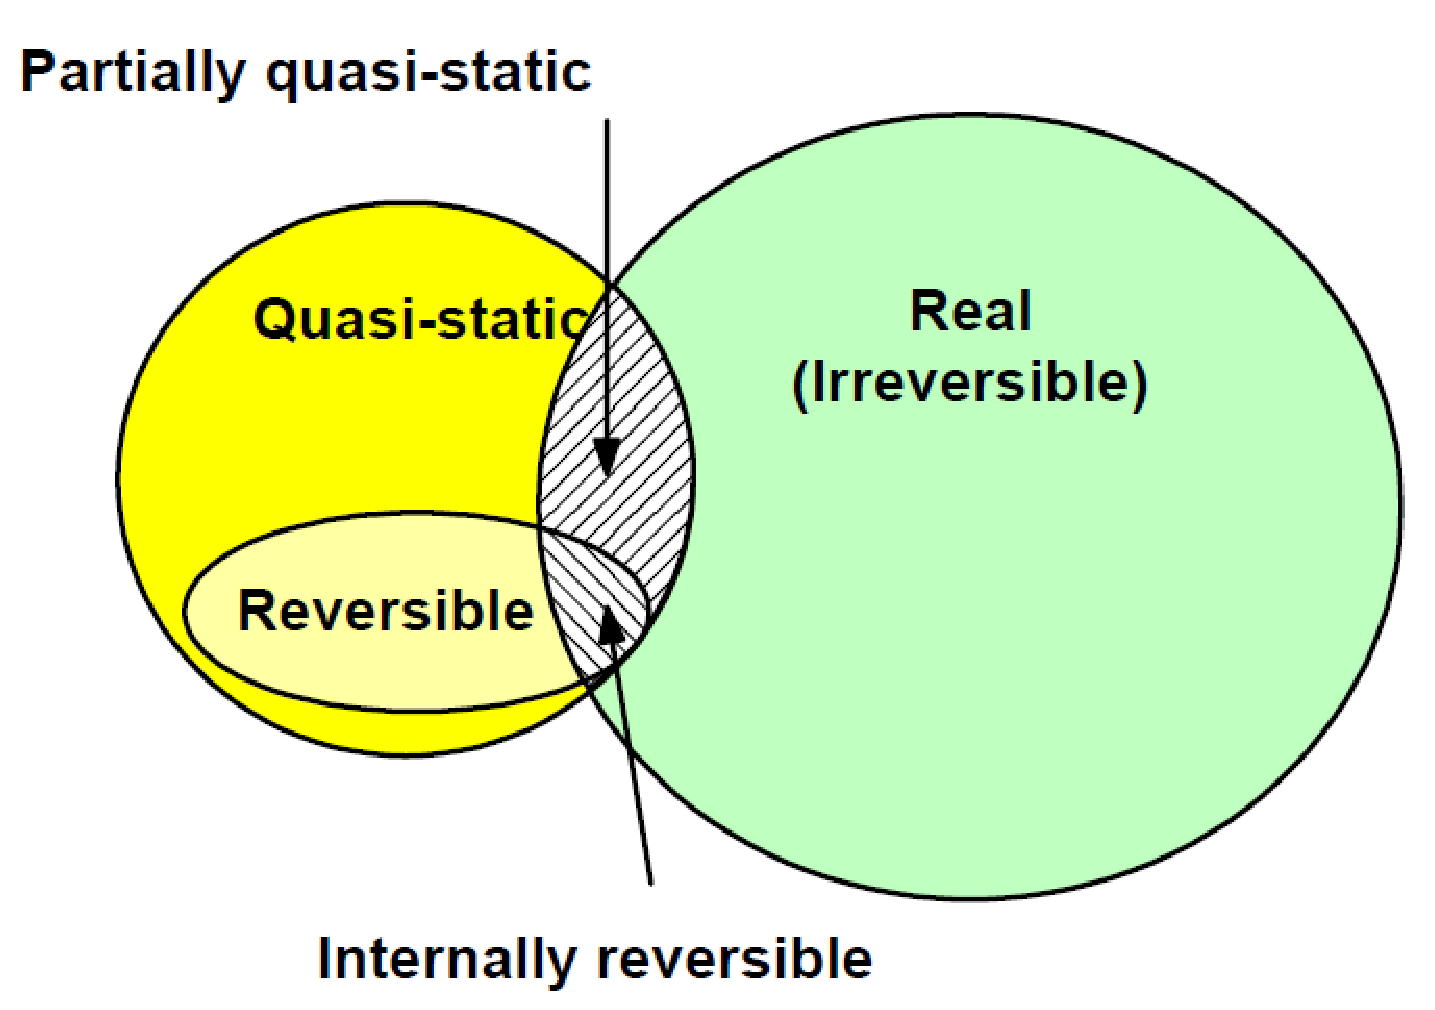
\includegraphics[height=5cm,
    angle=0]{./images/internal_reversible.eps}}
\caption{Two parts of the insular cortex (exposed by removing opercula): larger
anterior insular cortex (AIC) + smaller posterior insular cortex (PIC)}
\label{fig:insular-cortex}
\end{figure}

The insulae are believed to be involved in consciousness and play a role in
diverse functions usually linked to emotion or the regulation of the body's
homeostasis. One study on rhesus monkeys revealed widespread reciprocal
connections between the insular cortex and almost all subnuclei of the
amygdaloid complex




\subsection{Subgenual cortical area (Broadmann area 25, subgenual anterior
cingulate, subgenual cingulate)}
\label{sec:subgenual-cortical-area}	
\label{sec:broadmann-area-25}

Subgenual cortical area: originally in 1905, Brodmann labeled the area as part
of area 24. In 1909, he divided the area into area 24 and 25; and area 25 is
subgenual cortical area.

Subgenual cortical area (Broadmann area 25) is aka subgenual anterior cingualte
with rich expression of serotonin transporters (Sect.\ref{sec:serotonin-transporter}).
These transporter transport serotonin back to the presynaptic of serotonin
neurons (Sect.\ref{sec:serotonergic-neuron}).

\begin{enumerate}
  \item closely connected to the hippocampus (which involve in memory
  formation)
  \item to parts of frontal cortex (which involve in self-esteem)
\end{enumerate}

The region appears to be {\it overactive in treatment-resistant depression}.


\section{-- Cortical ensembles}
\label{sec:cortical-ensembles}

Similar to the concept of building block for the to ensemble myofibrils
(Sect.\ref{sec:contractile-unit})

\section{* White matter (of cerebral cortex, cerebrum)}
\label{sec:white-matter-cerebrum}
\label{sec:white-matter}

White matters resides below the cerebral cortex
(Sect.\ref{sec:cerebral_cortex}), and the different regions in the white
matters belong to the so-called {\it subcortical structures}
(Sect.\ref{sec:subcortical-structure}).

% 
% i.e. various ventricles and nuclei (e.g. caudate, putamen, globus
% pallidus), the thalamus, hypothalamus, cerebellum, internal capsule, brainstem, \ldots



\textcolor{red}{Neural types}: White matter consists mostly of myelinated nerve
cell processes (i.e. axons); thus carry nerve impulse between neurons in
different grey matter regions.

The white matter in the brain gets its color from a large number of myelinated
nerve cells. Unlike the grey matter, which peaks in development at the age of
20s, the white matter continue to develop in middle age.

\subsection{association fibers}
\label{sec:association-fibers}

 association fibers connect regions within the same hemisphere of the brain

\subsection{projection fibers}
\label{sec:projection-fibers}

projection fibers connect each region to other parts of the brain or to the
spinal cord

\subsection{commissural fibers or transverse fibers}
\label{sec:commissural-fibers}
\label{sec:transverse-fibers}

A commissure is the place where two things are joined. In anatomy, commissure
refers to a bundle of nerve fibers that cross the midline at their level of
origin or entry (as opposed to a decussation of fibers that cross obliquely). 

The commissural fibers or transverse fibers are coherent white-matter structures
that connect the two hemispheres of the brain.

Depending which parts of the two hemispheres are connected; the fibers can be
\begin{enumerate}
  \item callosal commissure (corpus callosum) - Sect.\ref{sec:corpus_callosum} 
  
  \item anterior commissure - Sect.\ref{sec:anterior-commissure}
  
  \item posterior commissure (epithalamic commissure) -
  Sect.\ref{sec:posterior-commisure}
\end{enumerate}

\subsection{-- posterior commissure (epithalamic commissure)}
\label{sec:posterior-commisure}

Posterior commissure connects the pretectal nuclei pretectal nuclei. It is
important in the bilateral pupillary light reflex, i.e.
a reflex that controls the diameter of the pupil, in response to the intensity
(luminance) of light.

\subsection{-- anterior commissure}
\label{sec:anterior-commissure}

A smaller band of nerve fibers called the {\bf anterior commissure} also
connects parts (which is  
\begin{enumerate}
  \item the two temporal lobes - Sect.\ref{sec:temporal-lobe}
  \item the two amygdala
\end{enumerate}
) of the cerebral hemispheres.

\subsection{-- Corpus callosum (callosal commissure)}
\label{sec:corpus_callosum}
\label{sec:callosal-commissure}

[NOTE: Latin: {\it corpus} = body, callosum = hard].

{\bf Corpus callosum} (or callosal commissure [commissure = the joint]) is the
largest white matter structure (Sect.\ref{sec:white-matter}, consisting 200-250
million axonal projections) connecting the two hemispheres of the human brain
(Sect.\ref{sec:cerebral-cortex}), Fig.\ref{fig:corpus_callosum}.

\begin{figure}[hbt]
  \centerline{
  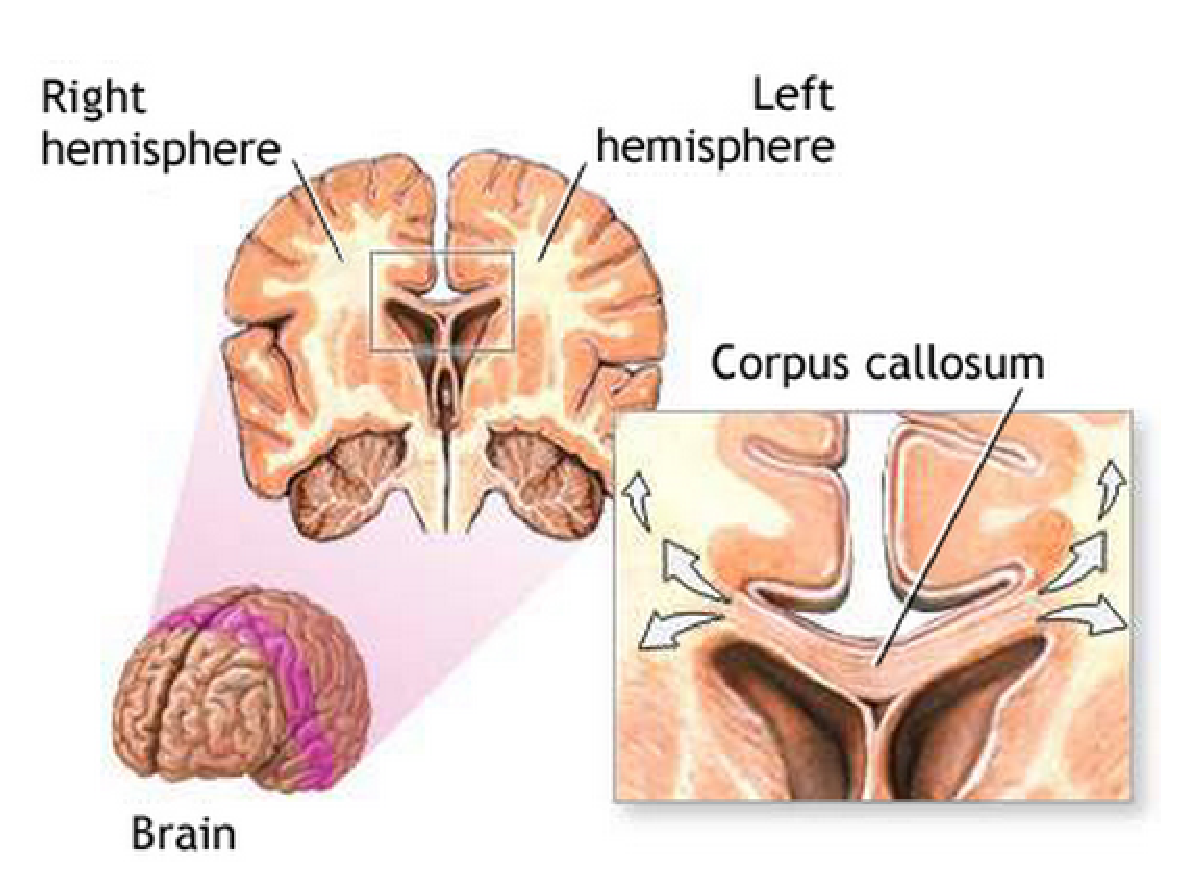
\includegraphics[height=4cm,
    angle=0]{./images/corpus_callosum_01.eps}
      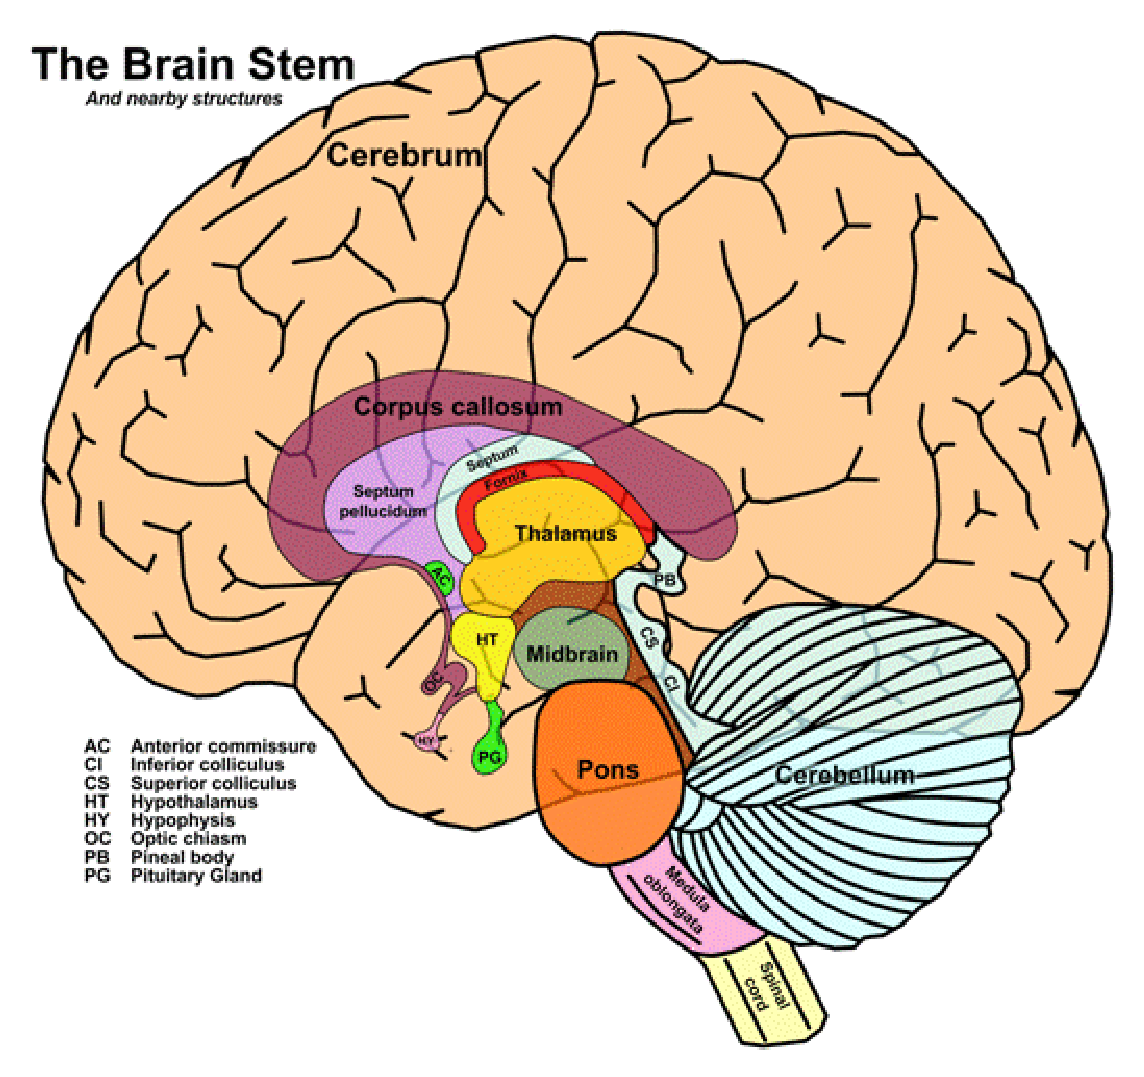
\includegraphics[height=5cm,
    angle=0]{./images/corpus_callosum_02.eps}}
  \centerline{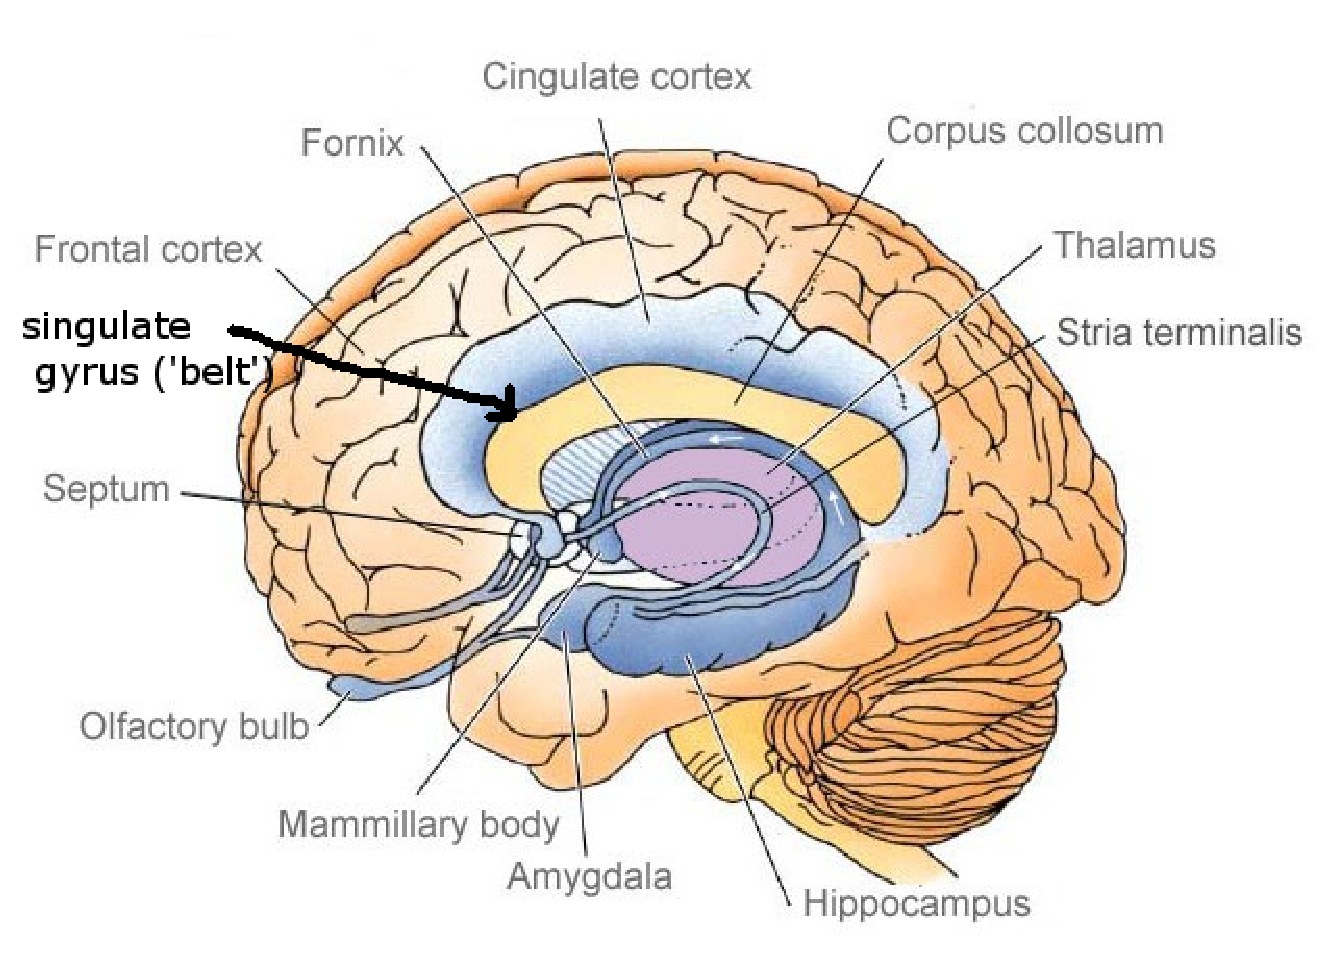
\includegraphics[height=6cm,
    angle=0]{./images/corpus_callosum_03.eps}}
\caption{Corpus callosum: (A) connecting the two hemisphere, (B) in relation to
other parts of the brain}
%http://www.nlm.nih.gov/medlineplus/ency/images/ency/fullsize/8753.jpg
%http://www.changedlivesnewjourneys.com/wp-content/uploads/Brain-Stem-Diagram.gif
%http://www.upright-health.com/images/limbic-system.jpg
\label{fig:corpus_callosum}
\end{figure}



References:
\begin{enumerate}
\item \url{http://www.macalester.edu/psychology/whathap/UBNRP/Split_Brain/Corpus Callosum.html}
\end{enumerate}

\subsection{Internal capsule}
\label{sec:internal_capsule}

The internal capsule is a subcortical large white matter.
It is a unique location where a large number of motor and sensory fibers travel
to and from the cortex.  The internal capsule divides the striatum
(Sect.\ref{sec:striatum}).

The portion of the internal capsule that links to the thalamus
(Sect.\ref{sec:thalamus}) is called {\it thalamic radiation}.

\url{http://stanfordmedicine25.stanford.edu/the25/ics.html}


\section{1.B. Subcortical structures}
\subsection{-- Olfactory bulb (rhinencephalon -
smell-brain) - (olfactory cortex - OC)}
\label{sec:olfactory-bulb}
\label{sec:olfactory-cortex}
\label{sec:rhinencephalon}

Olfactory system receives afferentation from olfactory epithelium, olfactory
tracts, and olfactory tubercles and handles smell signals. The odorant molecules
reaching the nasal cavity (i.e. the smell information) will be sensed by the
ordor receptors on the {\bf ordor receptor neurons} (ORNs) or olfactory sensory
neuron (OSNs) - Sect.\ref{sec:olfactory-nerve} (in the nasal cavity).

\begin{mdframed}
The other sensory inputs go to the reticular activating system (RAS -
Sect.\ref{sec:reticular-activating-system}).
\end{mdframed}

In the brain of mammals such as the cat, olfactory bulb is still important, but
the greatly expanded cerebrum (Sect.\ref{sec:cerebrum}) has assumed the higher
neural functions of correlation, association, and learning.
\begin{enumerate}
  \item glomerular layer - Sect.\ref{sec:glomerulus}
  
  \item bulbar circuitry
\end{enumerate}

The main olfactory epithelium of mammals lines the walls of the nasal cavity,
and samples the chemical composition of inhaled air via ORNS.
Such cells are then triggered a signal, via the receptor cells' extended axons
directly into the surface area called {\it glomeruli}
(Sect.\ref{sec:glomerulus}) of the highly organized olfactory bulb where many
neurites are present to receive the signals.

Unlike other sensing information, the olfactory signal does not goes through the
thalamus (Sect.\ref{sec:thalamus-function}) (Shepherd, 2005).
%Perception without a Thalamus: How Does Olfaction Do It? 

\subsection{Glomerulus (glomerular layer)}
\label{sec:glomerulus}

The glomerular layer (GL) region is occupied by three main types of
interneurons, periglomerular (PG) cells - Sect.\ref{sec:periglomerular-cell},
short-axon cells and external tufted (ET) cells - sometimes collectively
referred to as juxtaglomerular cells (Kratskin and Belluzzi, 2003; Panzanelli et
al., 2007). Dopaminergic neurons in the GL include PG cells (Kosaka et al.,
1985; Gall et al., 1987) and a fraction of ET cells (Halasz, 1990).

{\bf the glomerulus} (plural {\bf glomeruli}) is the many spherical structures
located in (and near the surface of) the olfactory bulb of the brain
(Sect.\ref{sec:olfactory-bulb}) where synapses form between the axonal terminals
of the ORNs and the dendrites of
\begin{itemize}
  \item mitral cells - Sect.\ref{sec:mitral-cell}
  
  \item tufted cells: the second type of projection neuron in the mammalian
  bulb, beside mitral cells.

  \item other cells:  external tufted cells, periglomerular cells,
  short axon cells, and astrocytes.
  
\end{itemize}
Once the signal is relayed in glumoleri, it is then transmitted to higher region
of the brain by mitral cells (Sect.\ref{sec:mitral-cell}).

At each glumolerus, the two ends of the synapses form the so-called 2
compartments: 
\begin{itemize}
  \item  the olfactory nerve zone: composed of preterminals and terminals of
  the ORNs
  
  \item and the non-olfactory nerve zone: composed of the dendritic processes of
  intrinsic neurons and is where dendrodendritic interactions between
  intrinsic neurons occur
\end{itemize}

In mammals, glomeruli typically range between 50-120 $\mum$ in diameter and
number between 1100 and 2400 depending on the species, with roughly between 1100
and 1200 in humans (and nearly absent in humans > 80 year old).


In mouse, there are  as many as 1000-1300 genes expressing ordorant receptors. 
The question is \textcolor{red}{\bf how many OR genes are expressed by a single
neuron?}. There have been different hypotheses 
\begin{enumerate}
  \item single neuron - single receptor.
  
  \item a single neuron expresses during differentiation zero, one, or a few OR
  genes
\end{enumerate}


\subsection{Striatum}
\label{sec:striatum}

The striatum is a subcortical region. Based on the origin of cortical
glutamatergic and midbrain dopaminergic (DA) afferents, the striatum can be
functionally divided into dorsal and ventral subregions. The dorsal striatum is
thought to be involved mostly in motor behaviors, while ventral striatum (or
nucleus accumbens, NAc) is crucial for motivational processes (Robbins and
Everitt, 1996; Groenewegen, 2003; Nestler, 2005).

Striatum is divided into ventral and dorsal subregions, based upon function and
connectivity
\begin{enumerate}
  \item dorsal striatum - Sect.\ref{sec:dorsal-striatum}
  \item ventral striatum - Sect.\ref{sec:ventral-striatum}
\end{enumerate}
Neuron types in this region is discussed in Sect.\ref{sec:striatal-neurons}.

The striatum is involved in the control of movement and action selection (Gerfen
and Surmeier, 2011). The striatum exerts this control by transforming excitatory
synaptic input from the cerebral cortex into patterned activity in two parallel
projection systems:
\begin{enumerate}
  \item direct pathway - Sect.\ref{sec:direct_movement_pathway}
  
  \item indirect pathway - Sect.\ref{sec:indirect_movement_pathway}
\end{enumerate}
Activity in direct pathway spiny projection neurons (dSPNs) promotes action,
whereas activity in indirect pathway spiny projection neurons (iSPNs) suppresses
action (Gerfen and Surmeier, 2011).


\subsection{Dorsal striatum (neostriatum): caudate nucleus (CN) and putamen
nucleus (Put)}
\label{sec:dorsal-striatum}
% \subsection{striatum (Caudate and Putamen [primates] vs. ventral striatum or
% nucleus accumbens [all mammals])}
\label{sec:caudate}
\label{sec:putamen}
\label{sec:neostriatum}


{\bf Dorsal striatum} (or simply {\bf striatum}, or neostriatum, or striate
nucleus) is considered a single functional structure. The term 'neo' suggests
the hypothesis that neostriatum developed later in evolution than globus
pallidus (Sect.\ref{sec:globus_pallidus}) - another region in basal ganglia.
\textcolor{blue}{From now on, when we talk about striatum, it
means dorsal striatum}. 

The striatum is by far the largest subcortical brain structure in the mammalian
brain, with an estimated volume of 10 cm$^3$ in the human brain (Schroeder et
al. 1975). Anatomical and interference studies suggest a functional
heterogeneity within striatum, i.e. it receives afferents from several cortical
and subcortical structures and projects to various basal ganglia nuclei.

The striatum in human is divided into caudate nucleus (CN) and putamen nucleus
(Put). The {\bf caudate}  and {\bf putamen} are functionally and
histologically similar nuclei located on either side of the internal capsule
(Sect.\ref{sec:internal_capsule}).

% The striatum in human is divided into caudate nucleus (CN) and putamen nucleus
% (Put) - see below. As being separated by the internal capsule
% (Sect.\ref{sec:internal_capsule}), the dorsal striatum is often referred to as
% two structures:
\begin{itemize}
  \item medial dorsal striatum or the {\bf caudate} : /KO-date/ (Latin: {\it
  cauda} = tail)

Sometimes a part of the caudate nucleus is referred to as the "knee" (genu).
  
  \item lateral dorsal striatum or the {\bf putamen}: /pyu-TA-mon/ (Latin: {\it
  caput} = head) 
\end{itemize}

% Collectively,
% they are called the dorsal {\bf striatum} (or {\bf striate nuclei}, the
% neostriatum). 
 
%There are three types of neurons found in striatum


As mentioned earlier, the excitatory
input
% It receives input from many brain areas beyond the basal ganglia, such as
% cerebral cortex, and limbic structures (e.g. amygdala, and hippocampus), but
% only sends output to other components of the basal ganglia.
\begin{verbatim}
cerebral cortex  -[excitatory]--> striatum
  (association cortex)     (caudate)
  (sensorimotor cortx)     (putamen)

limbic system   ----> striatum 
  (amygdala)           (caudate)        
  (hippocampal formation)     --> ventral striatum      
  
sensorimotor (only see, hear, touch) 
and motivational region --> thalamus (relay) -[excitatory]-->striatum

 NOTE: smell sensing (olfaction) does not go through thalamus
olfaction -------> limbic system

important modulatory afferents come from substantia nigra pars compacta
(dopamine) and the raphe nuclei (serotonin) in the midbrain
\end{verbatim}
NOTE: The sense of smell goes through a special nerve - olfactory nerve
(Sect.\ref{sec:olfactory-nerve}), and goes directly to the limbic system
(Sect.\ref{sec:limbic-system}). As a result, smell can trigger emotional
reactions much more easily than the other senses.
The onslaught of a long forgotten memory brought about by a particular smell is
sometimes referred to as a "Proustian memory" because author Marcel Proust so
richly described the experience.



The different signaling pathways is given in
Fig.\ref{fig:corticostriato-thalamo-cortical-pathway}.
%Fig.\ref{fig:striatum-signaling_pathways}.
The striatum projects to the medial and lateral segments of the globus pallidus
(Sect.\ref{sec:globus_pallidus}) as well as to the substantia nigra pars
reticulata (SNr - Sect.\ref{sec:SNr}).
\textcolor{red}{The striatum inhibits the internal segment of the Globus
Pallidus (GPi), which would normally inhibit thalamus.  Since the internal
segment of GPi is being inhibited, it will not inhibit thalamus, which means
thalamus can excite cortex (primary motor cortex for example) and cause
movement.}

% \begin{figure}[hbt]
%   \centerline{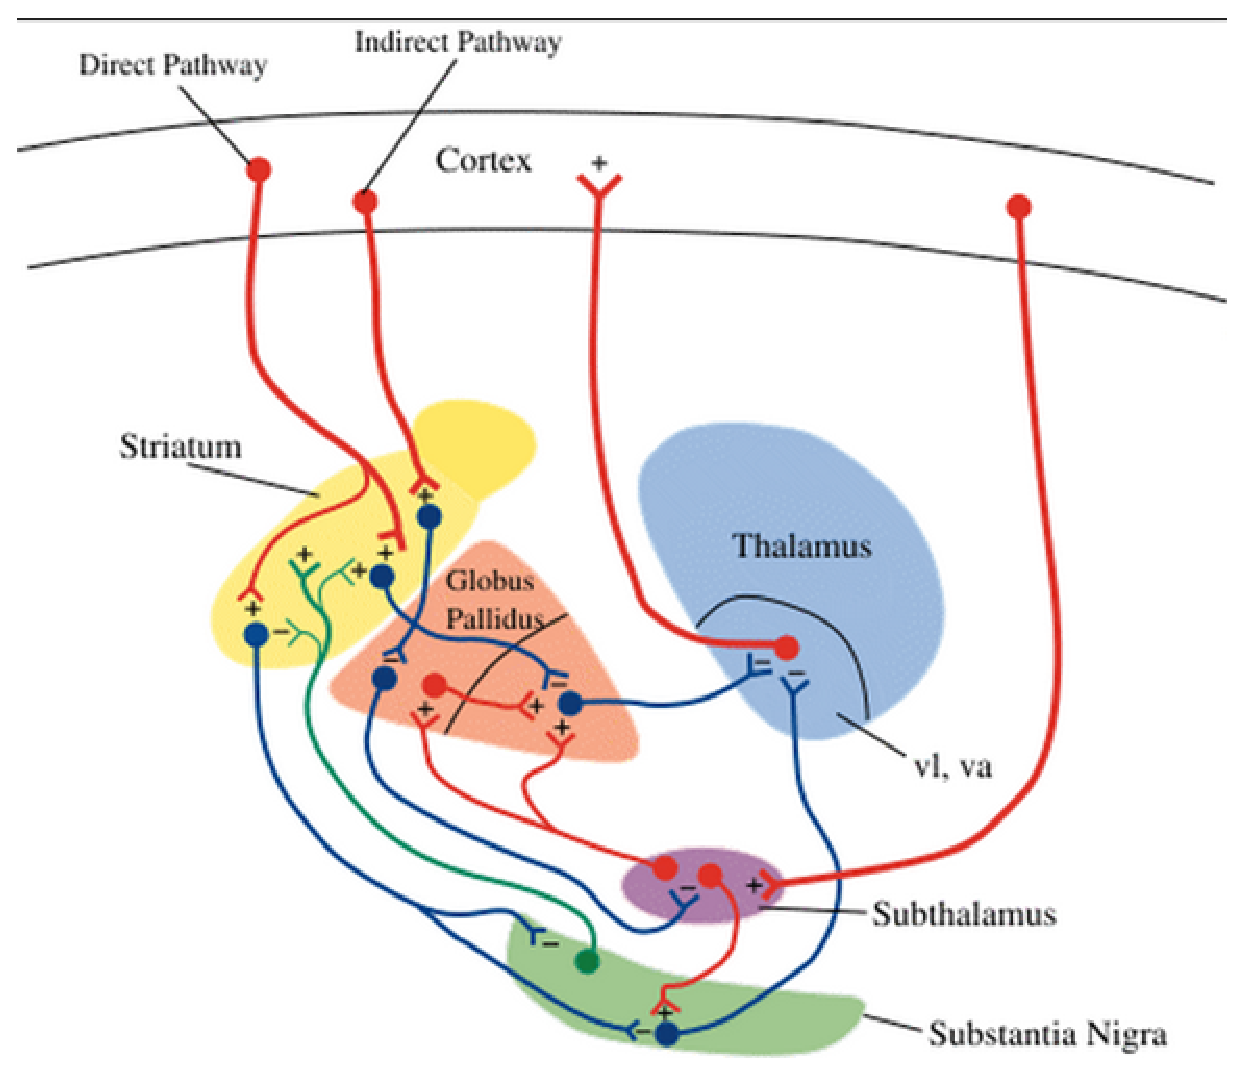
\includegraphics[height=8cm,
%     angle=0]{./images/striatum_signaling_pathways.eps}}
% \caption{cortico-striato-thalamo-cortical or the cortico-striato-pallido-thalamo-cortical pathway. }
% \label{fig:striatum-signaling_pathways}
% %\url{http://radiopaedia.org/articles/posterior-cerebral-artery}
% \end{figure}


\url{https://www.dartmouth.edu/~rswenson/NeuroSci/chapter_8C.html}


\subsection{-- patch/striosomes and matrix}
\label{sec:striosomes-striatum}
\label{sec:matrix-striatum}
\label{sec:patche-striatum}

The striatum is subdivided into sectors along a ventromedial-dorsolateral
continuum largely on the basis of external connectivity.

All regions of the striatum are divided further into regions of patch/striosomes
and matrix, again on the basis of differential connectivity and distribution of
neurochemical markers (Desban et al., 1993).

The two striatal compartments, the striosomes (or patches) and the matrix, are
distinguished by several biochemical markers, and their afferent
and efferent connections. 
\begin{itemize}
  \item patch/strisome region: projecting to SNc, i.e. inhibiting the DA neurons
  in this region
  
  \item matrix: divided into projecting to direct pathway and indirect pathway
\end{itemize}


\subsection{Ventral striatum}
\label{sec:ventral-striatum}

The ventral striatum (VS) is the striatal region most closely associated with
reward (Sect.\ref{sec:reward-system}).
It receives its primary input from the orbital prefrontal cortex, insular
cortex, and cingulate cortex. These cortical areas, particularly orbital and
insular cortex, receive sensory information from all modalities. 

The ventral striatum includes
\begin{itemize}
  \item nucleus accumbens core (NAcc) - Sect.\ref{sec:nucleus_accumbens}
  
  \item olfactory tubercle
  
  \item islands of Calleja: in non-primate species
\end{itemize}
Among these, only the NAc is part of the basal ganglia
(Sect.\ref{sec:basal-ganglia}).

% Ventral striatums (nucleus accumbens, NAc) receives excitatory input
% from both frontal cortex and limbic region (e.g. thalamus). 

\subsection{-- Nucleus accumbens (NAc, NAcc, NAcb)}
\label{sec:nucleus_accumbens}

The nucleus accumbens (NAc, NAcb) is part of the ventral striatum in the basal
ganglia.
It serves as a link between the basal ganglia and the limbic system.
The nucleus accumbens (NAc, NAcb,  accumbens nucleus or as the nucleus accumbens
{\it septi} (Latin for nucleus adjacent to the septum)) looks like a patch and
connects the caudate to the putamen, rostrally in the brain. This is thought to
aid motor selection and motor memory.

INPUTS: NAc receives projection from neurons in
\begin{enumerate}
  \item prefrontal cortex (i.e. Glutamate as neurotransmitter)
  \item basolateral amygdala (Sect.\ref{sec:amygdala})
  \item VTA (i.e. domapine as neurotransmitter) - connect via mesolimbic pathway
  (Sect.\ref{sec:mesolimbic-pathway})

  \item CA1 hippocampus and ventral subiculum of hippocampus: to dorsomedial
  area of NAc

Help depolarize the Vm - making the neurons in NAc more excitable.
Even though subiculum neurons are found to hyperpolarize (increase negativity);
CA1 neurons "ripple" (fire > 50 Hz) in order to accomplish this positive net
effect.

  \item the tuberomammillary nucleus via histaminergic projections (the sole
  source of histamine neuron)
\end{enumerate}

OUTPUTS: Depending on the cell types (see below), the neurons in NAc can send
axonal projections to
\begin{enumerate}
  \item basal ganglia  (Sect.\ref{sec:basal-ganglia})
  \item ventral analog of globus pallidus (Sect.\ref{sec:ventral-pallidum})
  \item tail of VTA (Sect.\ref{sec:ventral-tegmented-area})
  \item substantia nigra (Sect.\ref{sec:substantia_nigra})
  \item reticular formation of pons (Sect.\ref{sec:reticular-formation})
\end{enumerate}

NAc can be further divided into shell and core regions, which differ in their
input (including morphology and functions due to different in neuron
subpopulation within each region).
\begin{enumerate}
  \item {\bf NAc shell} (the outer region of NAc): it is considered
  \textcolor{red}{part of the extended amygdala} (Sect.\ref{sec:amygdala}). 
  
  The shell neurons project to the subcommissural part of the ventral pallidum
  as well as the ventral tegmental area and to extensive areas in the
  hypothalamus and extended amygdala.
  
  \item {\bf NAc core} (the inner region of NAc): it is \textcolor{red}{part of
  the ventral striatum} (located within basal ganglia) -
  Sect.\ref{sec:ventral-striatum}
  
  The core neurons project to other sub-cortical areas such as the globus
  pallidus and the substantia nigra.
\end{enumerate}

The neurons here are 
\begin{itemize}
  \item 95\% neurons in NAc are medium spiny neurons
(Sect.\ref{sec:MSN-in-NAc}).
   
  \item About 1-2\% of the remaining neuronal types are large aspiny cholinergic
interneurons (Sect.\ref{sec:cholinergic_neurons}) and another 1-2\% are
GABAergic interneurons (Sect.\ref{sec:interneurons}).

\end{itemize}

\begin{mdframed}
{\bf Striatum} is the largest nucleus in the basal ganglia
(Sect.\ref{sec:basal-ganglia}). It comprises \citep{gerfen1996, voorn2004}

\begin{itemize}
  \item (in primate): caudate nucleus and putamen
  \item (all mammals): ventral striatum (mainly core nucleus accumbens) and
  shell nucleus accumbens
\end{itemize}

\end{mdframed}

\subsection{globus pallidus (GPi (GPm), GPe) - dorsal pallidum (in primates) ==
ventral pallidum (VP) (in non-primates)}
\label{sec:globus_pallidus}
\label{sec:dorsal-pallidum}
\label{sec:ventral-pallidum}

Ventral pallidum (VP) is the terms refer to globus pallidus
(Sect.\ref{sec:globus_pallidus}) for non-primates, i.e. the ventral analog of
globus pallidus.
The {\bf globus pallidus} (GP) is aka {\it dorsal pallidum} (terms used in
primates), {\it paleostriatum}). (Latin: pale globe, a pale[light
color]-appearing spherical area in the brain). The term 'paleo' (old) suggests
the hypothesis that GP developed earlier in evolution than the "neostriatum" or
striatum (Sect.\ref{sec:neostriatum}).

INPUT:
\begin{verbatim}
NAc --> VP
\end{verbatim}
Sect.\ref{sec:nucleus_accumbens}.

OUTPUT:
\begin{verbatim}
VP --> medial dorsal nucleus of the dorsal thalamus --> 
                 (1) prefrontal cortex
                 (2) striatum 
\end{verbatim}


GP neurons (Sect.\ref{sec:Pallidal-neurons}) spontaneous firing sends inhibitory
output to a number of motor-related areas.
This inhibitory activity is blocked by the inhibitory input from the (dorsal)
striatum via inhibitory GABAergic neurons that are tonically active
(Sect.\ref{sec:GABA}).

Developmentally, the globus pallidus is a part of the diencephalon
(Sect.\ref{sec:diencephalon}) that has migrated to the telencephalon
(Sect.\ref{sec:telencephalon}), but it is still considered amongst the basal
ganglia.
\begin{itemize}
  \item GP (paleostriatum) is part of lentiform nucleus
  (Sect.\ref{sec:lenticular_nucleus}) which is part of the striate body, a
  component of the basal ganglia (Sect.\ref{sec:basal-ganglia})
\end{itemize}

The globus pallidus, itself, is divided by the internal medullary lamina
(Sect.\ref{sec:thalamus}) into two components
\begin{enumerate}
  \item internal: a medial (internal) segment {\bf GPi} (or {\bf GPm}) 

  NOTE: The term GPi is used in primates; while in cats and rodents is known as
  the {\bf entopeduncular nucleus}. 

  \item external: lateral (external) segment {\bf GPe}. 
  
%In non-primat
\end{enumerate}

Both GPi and GPe shares the similar morphology and a common neurotransmitter,
GABA, yet they are distinct in function. GPe has strong connection with STN
(Sect.\ref{sec:STN}), and GPe is a part of the indirect pathway
(Sect.\ref{sec:indirect_movement_pathway}), while the GPi is a component in both
the direct and indirect pathways (Sect.\ref{sec:direct_movement_pathway}).


\subsection{-- GPi (GPm): pars interna}
\label{sec:GPi}
\label{sec:GPm}

Globus pallidus pars interna (GPi)

GPi and SNr (Sect.\ref{sec:SNr}) both receives input from striatum, and are
part of the direct signaling pathways (Sect.\ref{sec:direct_movement_pathway}).
The GPi has strong interactions with the motor cortices and controls
somato-motor behaviors. On the other hand, the SNr has interactions with the
prefrontal cortex and is considered to control associative functions.

The GPi and SNr are the output nuclei of the basal ganglia and relay the final
signals to the thalamus. GPi neurons fire spontaneously at high frequency
(10-110 Hz) without pauses. All GPi neurons use GABA as their neurotransmitters.

\subsection{-- GPe: pars externa}
\label{sec:GPe}

Only recently have studies addressed the problem - GPe are more heterogeneous
than previously appreciated - by correlating electrophysiological properties of
GPe neurons with objective criteria, such as their genetic signatures and
projection targets (Mallet et al., 2012; Mastro et al., 2014; Abdi et al., 2015;
Dodson et al., 2015).

Recent studies have challenged the idea that the GPe comprises a single,
homogenous population of neurons that serves as a simple relay in the indirect
pathway. However, we still lack a full understanding of the diversity of the
neurons that make up the GPe.
\begin{enumerate}
  
  \item PV-IRES-Cre driver line was obtained from The Jackson Laboratory
  (Hippenmeyer et al., 2005) and crossed with a floxed-stop tdTomato reporter
  line (Jackson Laboratory; Madisen et al., 2010) to generate PV-tdTom mice.
  
  \item  Lhx6-eGFP and ChAT-Cre mice were generated from the GENSAT project
  (Gong et al., 2003; Gerfen et al., 2013).
  
  \item  ChAT-Cre line was crossed with the floxed-stop tdTomato reporter line
  to generate ChAT-tdTom mice. 
  
  \item Npas1 knock-out mice (Erbel-Sieler et al., 2004) were obtained from Dr.
  John Rubenstein (University of California, San Francisco, San Francisco, CA).
  
  \item Mice harboring targeted disruption in Kcnd2 (Kv4.2-/-) or Kcnd3
  (Kv4.3-/-; Guo et al., 2005; Burkhalter et al., 2006; Norris and Nerbonne,
  2010; Carrasquillo et al., 2012) were obtained from Dr. Jeanne Nerbonne
  (Washington University in St. Louis, St. Louis, MO).
  
Double Kv4-null mutants (Kv4.2-/- and Kv4.3-/-) were used to confirm the
molecular identity of channels underlying the transient, Kv4-like K+ current in
GPe neurons.

  \item novel multicistronic {\bf Npas1-Cre-2A-tdTomato} BAC transgenic mouse
  line (aka Npas1-tdTom for simplicity):  using regulatory elements of {\it
  Npas1} gene (Vivian et al., 2015).

NOTE: C57BL/6J wild-type mice (Jackson Laboratory) were used in a subset of
  experiments. Both male and female mice were used in this study.
  
Using a combinatorial transgenic and immunohistochemical approach, we discovered
that parvalbumin-expressing neurons (PV+-neuron: 55\%) and Npas1-expressing
neurons (27\%) in the GPe represent two nonoverlapping cell classes.
These two genetically identified cell classes projected primarily to the
subthalamic nucleus and to the striatum, respectively.
A third calss of GPe neuron classes were characterized based on their expression
of Lhx6, Foxp2, and choline acetyltransferase (ChAT).

The two neurons types are distinct in their autonomous and driven firing
characteristics, their expression of intrinsic ion conductances, and their
responsiveness to chronic 6-hydroxydopamine lesion.
 
\end{enumerate}


Globus pallidus pars externa (GPe) has two main subpopulations of GABAergic cell
types: "GP-TI" and "GP-TA" (Mallet et al., 2008a)) readily distinguished by
their distinct temporal activities, such as preferentially firing at different
phases of the exaggerated beta-frequency (15-30 Hz) oscillations that accompany
movement difficulties in PD patients and this animal model (Brown et al., 2001;
Hammond et al., 2007; Mallet et al., 2008a, 2008b).

\begin{enumerate}
  \item {\bf prototypic neurons} (GP-TI neurons, often PV+-neurons; fast-firing
  (tonic firing or tonic activated)): 55\% number in GPe, innervate
  downstream BG nuclei (i.e. project GABAergic synapses to STN)
  
  Prototypic neurons fire antiphase to STN neurons.
  
  
  
  \item {\bf arkypallidal neurons} (GP-TA neurons, preproenkephalin,
  Npas1-expressing neurons, 27\% number in GPe):  innervate upstread BG nuclei
  (i.e. project (only) GABergic/enkephalinergic to D1/D2 MSNs in striatum),
  autonomous (tonic) firing.
  
Arkypallidal neurons fire in-phase with STN neurons

  
NOTE: autonomous firing in Npas1+ neurons was reduced in a chronic
6-hydroxydopamine (6-OHDA) lesion model of PD.

  \item A third calss of GPe neuron classes were characterized based on their
  expression of Lhx6, Foxp2, and choline acetyltransferase (ChAT):
   Lhx6-expressing (Lhx6+) neurons account for the remaining unidentified
   GPe neurons, i.e. 30\%.
   
   Approximately half of these coexpressed either Npas1 or PV (Npas1+ = 26 $\pm$
   8\%, n = 1140 neurons; PV+ = 27 $\pm$ 7\%, n = 619 neurons).
   The remaining fraction, which was devoid of Npas1 and PV expression,
   represented $\approx$ 14\% of total GPe neurons.
\end{enumerate}


GPe and STN (Sect.\ref{sec:STN}) project to the cerebral cortex through the
thalamus (Sect.\ref{sec:thalamus})


\subsection{Substantia nigra (SNc, SNr)}   
\label{sec:substantia_nigra}

The substantia nigra (found in the midbrain) is a part of the basal ganglia
(Sect.\ref{sec:basal-ganglia}).  Humans have two substantia nigra, one on each
side of the midline.

Each {\bf substantia nigra} consists of 2 parts with very different connections
and functions:
\begin{enumerate}
  \item substantia nigra {\bf pars compacta} (SNc, SNpc): contains mainly
  dopaminergic neurons (Sect.\ref{sec:dopaminegic_neurons})
  
  \item substantia nigra {\bf pars reticula} (SNr, Sect.\ref{sec:SNr}): contains
  mainly GABAergic neurons (Sect.\ref{sec:GABAergic-neurons})
\end{enumerate}
Sometimes, a third region, the {\bf pars lateralis}, is mentioned, though it is
usually classified as part of the pars reticulata.

\subsection{-- substantia nigra pars reticulata (SNr, SNpr)}
\label{sec:SNr}
\label{sec:SNpr}

The {\bf substantia nigra pars reticulata} (SNr, SNpr) (Latin: black substance)
is part of the substantia nigra (Sect.\ref{sec:substantia_nigra}) and involves
in both 
\begin{itemize}
  \item  direct movement pathways (Sect.\ref{sec:direct_movement_pathway})
where it receives the striatal output as the GABA neurotransmitter,
which plays an important role in basal ganglia function.

  \item indirect movement pathways (Sect.\ref{sec:indirect_movement_pathway})
where it receives the output from subthalamus nucleus (STN - Sect.\ref{sec:STN}) 
\end{itemize}
Check Fig.\ref{fig:corticostriato-thalamo-cortical-pathway}.


\subsection{-- Substantia nigra pars compacta (SNc, SNpc)}
\label{sec:SNpc}
\label{sec:SNc}

The {\bf substantia nigra pars compacta} (SNc, SNpc) is part of the substantia
nigra (Sect.\ref{sec:substantia_nigra}).

The doparminergic neurons (Sect.\ref{sec:dopaminegic_neurons}) in substantia
nigra pars compacta (SNc, SNpc), projects to the striatum via excitatory synapse
using dopamine as neurotransmitters (Sect.\ref{sec:dopamine}).
These neurons are death in Parkinson disease (Sect.\ref{sec:Parkinson-disease}).

\subsection{subthalamic nucleus (STN)}
\label{sec:STN}
\label{sec:subthalamic_nucleus-neurons}

The subthalamic nucleus (STN) is composed of glutamatergic
neurons (Sect.\ref{sec:glutamatergic_neurons}) which control the circuitry of
the basal ganglia (Sect.\ref{sec:basal-ganglia}). These principal neurons have
rather long sparsely spiny dendrites.
 

STN is not an output structure; instead it modulate the activity of the two
principal output structures of the network: GPi (Sect.\ref{sec:GPi}) and SNr
(Sect.\ref{sec:substantia_nigra}).
As shown in Fig.\ref{fig:corticostriato-thalamo-cortical-pathway}, the output of
STN regulates GPi and SNr as part of the indirect movement pathways
(Sect.\ref{sec:indirect_movement_pathway}).

In rat brain slices, a substantial proportion of STN neurons can shift from a
regular single-spike mode to a burst-firing mode \citep{beurrier1999}.



\section{2. Cerebellum (little brain - motor + cognitive)}
\label{sec:cerebellum}


{\bf Cerebellum} is the little brain, yet playing important role in motor
control (Sect.\ref{sec:motor-pathway}), and involving in some cognitive
functions (attention, language) and probably some emotional functions (fear,
pleasure response) - Sect.\ref{sec:cerebellum}). 
As the {\bf cerebellum} grows out of the same vesicle that the pons
(Sect.\ref{sec:pons}) grows out, it is connected to and continuous with the rest
of the brain via the pons. The main function of the cerebellum is listed below.

\begin{itemize}
  \item Maintenance of balance and posture:
get input from vestibular receptors (Sect.\ref{sec:vestibular_receptor}) and
proprioceptors (Sect.\ref{sec:proprioceptor})

  \item Coordination of voluntary movements: as most muscle movements
  requires the temporal coordination of different muscle groups, the
  function here is to coordinate the timing and force of these different muscle
  groups to produce fluid limb or body movements.
  
  \item motor learning: adapting and fine-tuning motor programs to make accurate
  movements through a trial-and-error process.
  
  \item Cognitive functions: involves in certain cognitive functions, e.g.
  language.
\end{itemize}
% Like the basal ganglia (Sect.\ref{sec:basal-ganglia}, the
% cerebellum is historically considered as part of the motor system, but its
% functions extend beyond motor control in ways that are not yet well understood.

\begin{figure}[hbt]
  \centerline{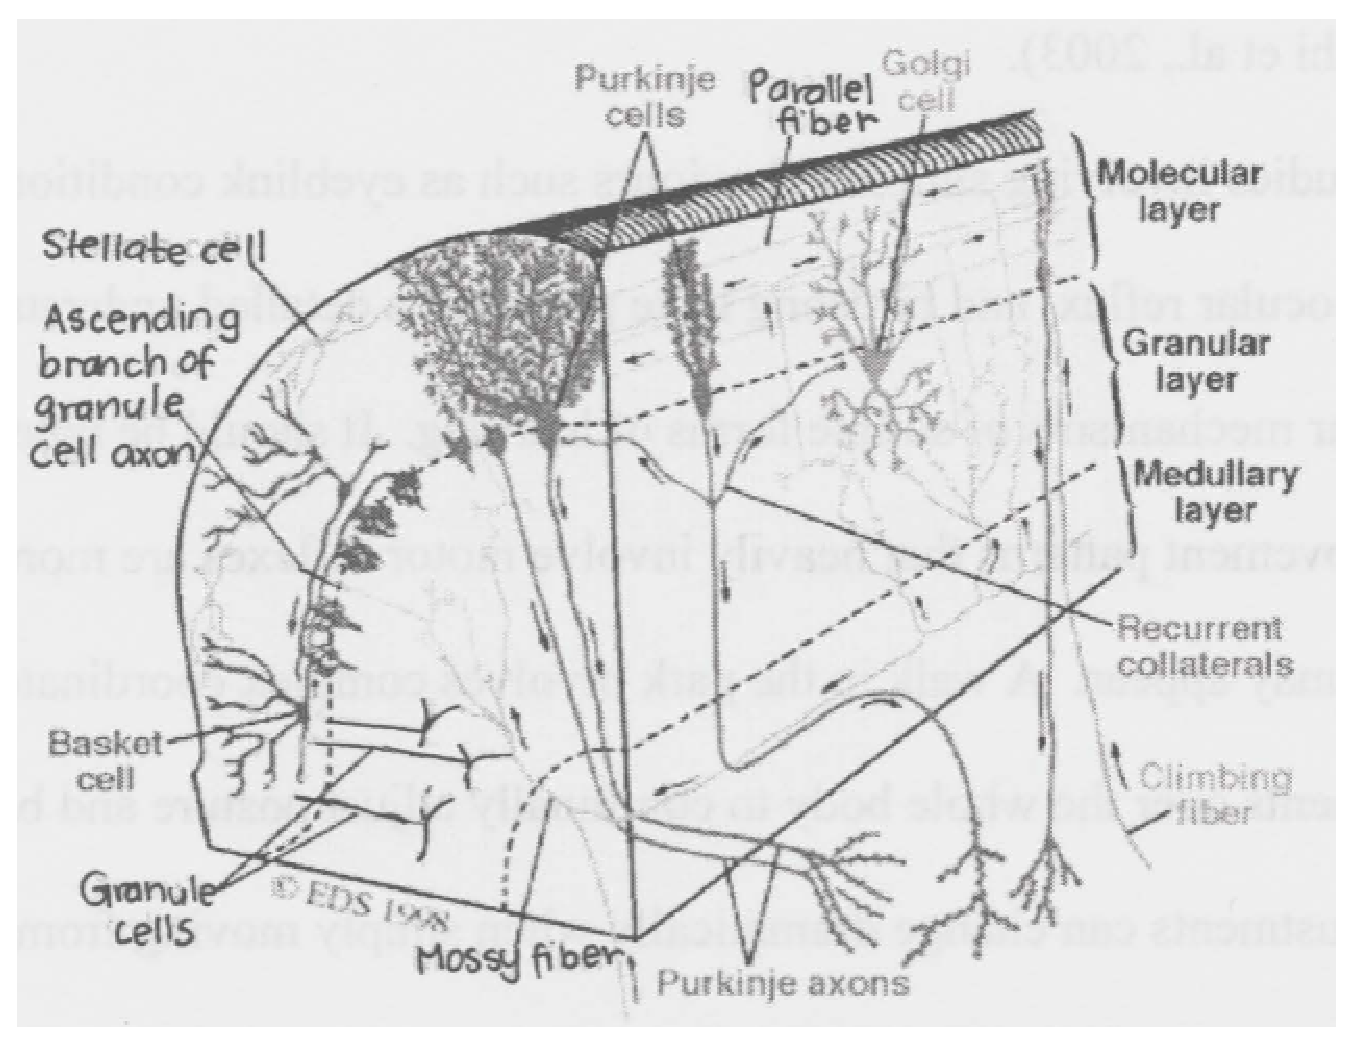
\includegraphics[height=5cm,
    angle=0]{./images/cerebellum.eps},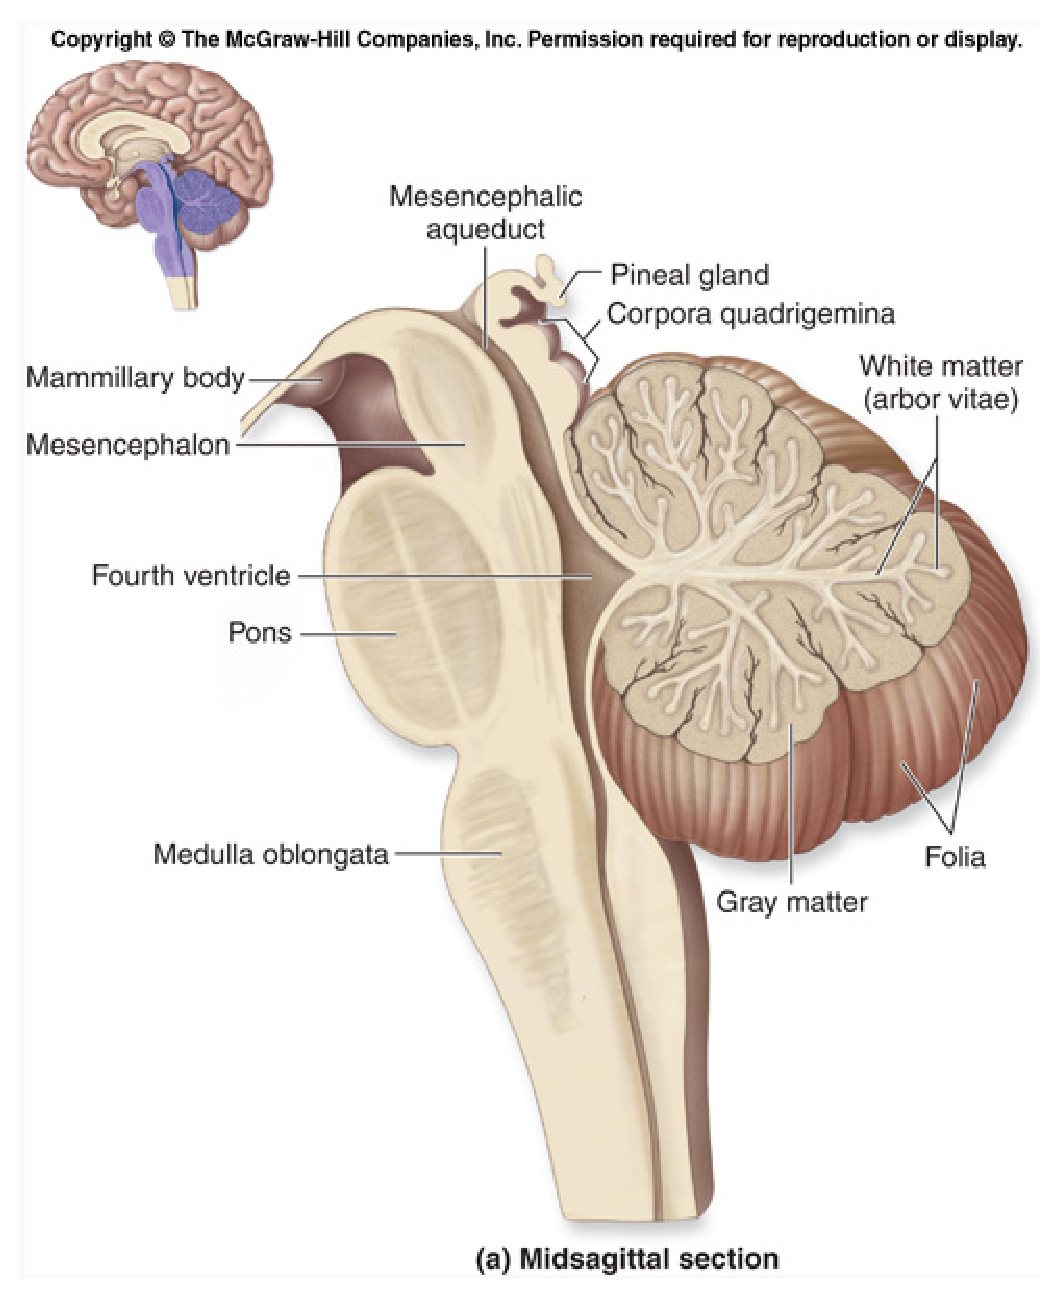
\includegraphics[height=8cm,
    angle=0]{./images/brain_10.eps}}
  \caption{(A) The various cell types in the cerebellum. (B) The location of the
  cerebellum in relation to other parts of the brain:
  mammillary body, mesencephalon (midbrain), mesencephalic aqueduct, pineal
  gland, corpoa quadrigemina, white matter (arbor vitae), grey matter, folia,
  fourth ventricle, pons, medulla oblongata}
\label{fig:cerebellum_position}
\end{figure}

Even though it was called ``little brain'' (as it accounts only for about
10\% of the brain volume), recent discoveries have revealed the powerful
features of this region, which is considered as the powerful computer functioning as a
coordinator. 
\textcolor{red}{In particular, cerebellum contains more nerve cells than any
other regions (as it contains more than 50\% of the total neurons in
the brain)},
Fig.\ref{fig:cerebellum_position}(A)
\footnote{\url{http://www.newhorizons.org/neuro/leiner.htm}}.
\begin{itemize}
  
  \item a single layer of Purkinje cells (Sect.\ref{sec:Purkinjie_nerves}):
  project on the neurons of the dentate nuclei of the cerebellum, and receive
  input from the {\bf climbing fiber} (axons of the inferior olive's neurons)

INPUT  
\begin{verbatim}
inferior olive --[axon=climbing fiber]---> Purkinje cell
\end{verbatim}
  The dendritic branches of each Purkinje cell receive excitatory synapses from
  the branch terminations of a single afferent climbing fibre which are axons
  of the neurons in inferior olive (Sect.\ref{sec:medulla_oblongata}).

  \item small granular cells (Sect.\ref{sec:granule_cells}) in the deep layer of
  the cerebellum: its axons ascend and project  into the surface layer of the
  cerebellum (the cerebellar cortex) where they branch to form the {\bf parallel
  fibres}, and receive input from the {\bf mossy fibres} (axons of neurons in
  the pontine nuclei that receive information from the cerebral cortex), act in a highly
  diffuse fashion.
  
INPUT  
\begin{verbatim}
pontine nuclei --[axon=mossy fiber]---> small granular cells --
     --[parallel fiber]--->
\end{verbatim}

The parallel fibres run perpendicular to the Purkinje cell dendrites, thus
crossing many Purkinje cells and connecting with each in turn.
Though each parallel fibre makes only one contact with each Purkinje cell that
it crosses, it makes contact with a huge number of such cells along its path,
which measures just a few millimeters.

\end{itemize}
In addition, it can process information more quickly than other parts of the
brain.
Finally, it has a huge number of connections to the cerebral cortex, i.e. 40
millions nerve fibres; which is 40 times greater than the connection from optic
fibres that connect the optic tract to human brain.  The anatomy of the
cerebellum is shown in Fig.~\ref{fig:cerebellum_anatomy}.

Cerebellum locates at the back of the brain, underlying the occipital lobe and
temporal lobe of the neocortex, Fig.\ref{fig:cerebellum_position}(B). It is
relatively well-protected from trauma compared to the temporal lobe, frontal
lobe and brain
stem\footnote{\url{http://www.neuroskills.com/tbi/bcerebel.shtml}}.

% As the main functionality is for motor movement, balance and equilibrium and
% muscle tone, however, the motor commands are not initiated from the cerebellum;
% rather, the cerebellum only modify the motor commands to make the movements more
% adaptive and accurate. 


\begin{figure}[hbt]
  \centerline{
  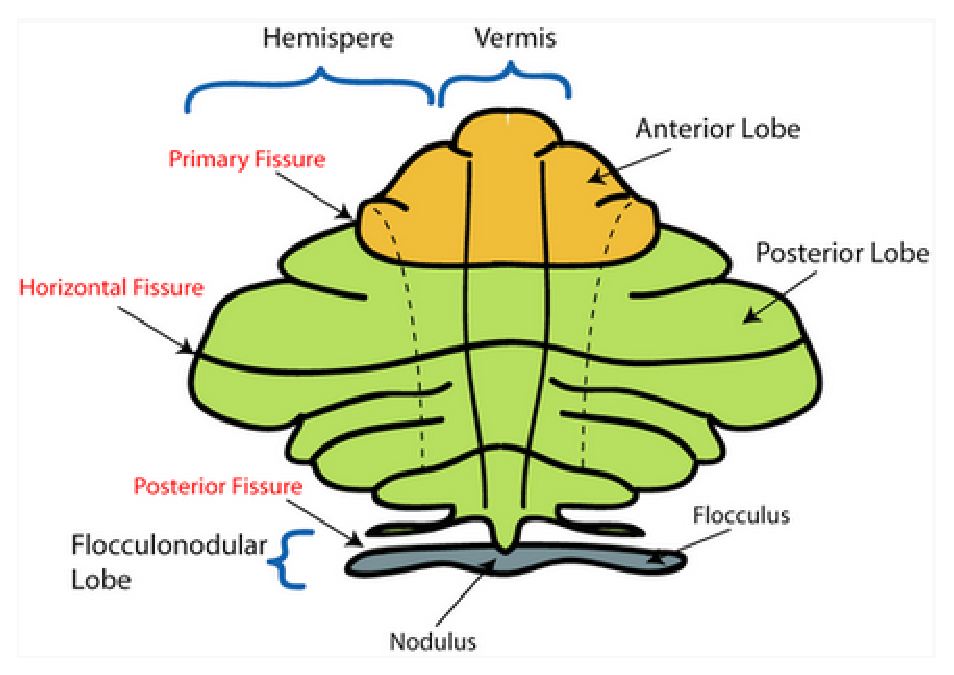
\includegraphics[height=4cm,
    angle=0]{./images/cerebellum_lobes.eps}
  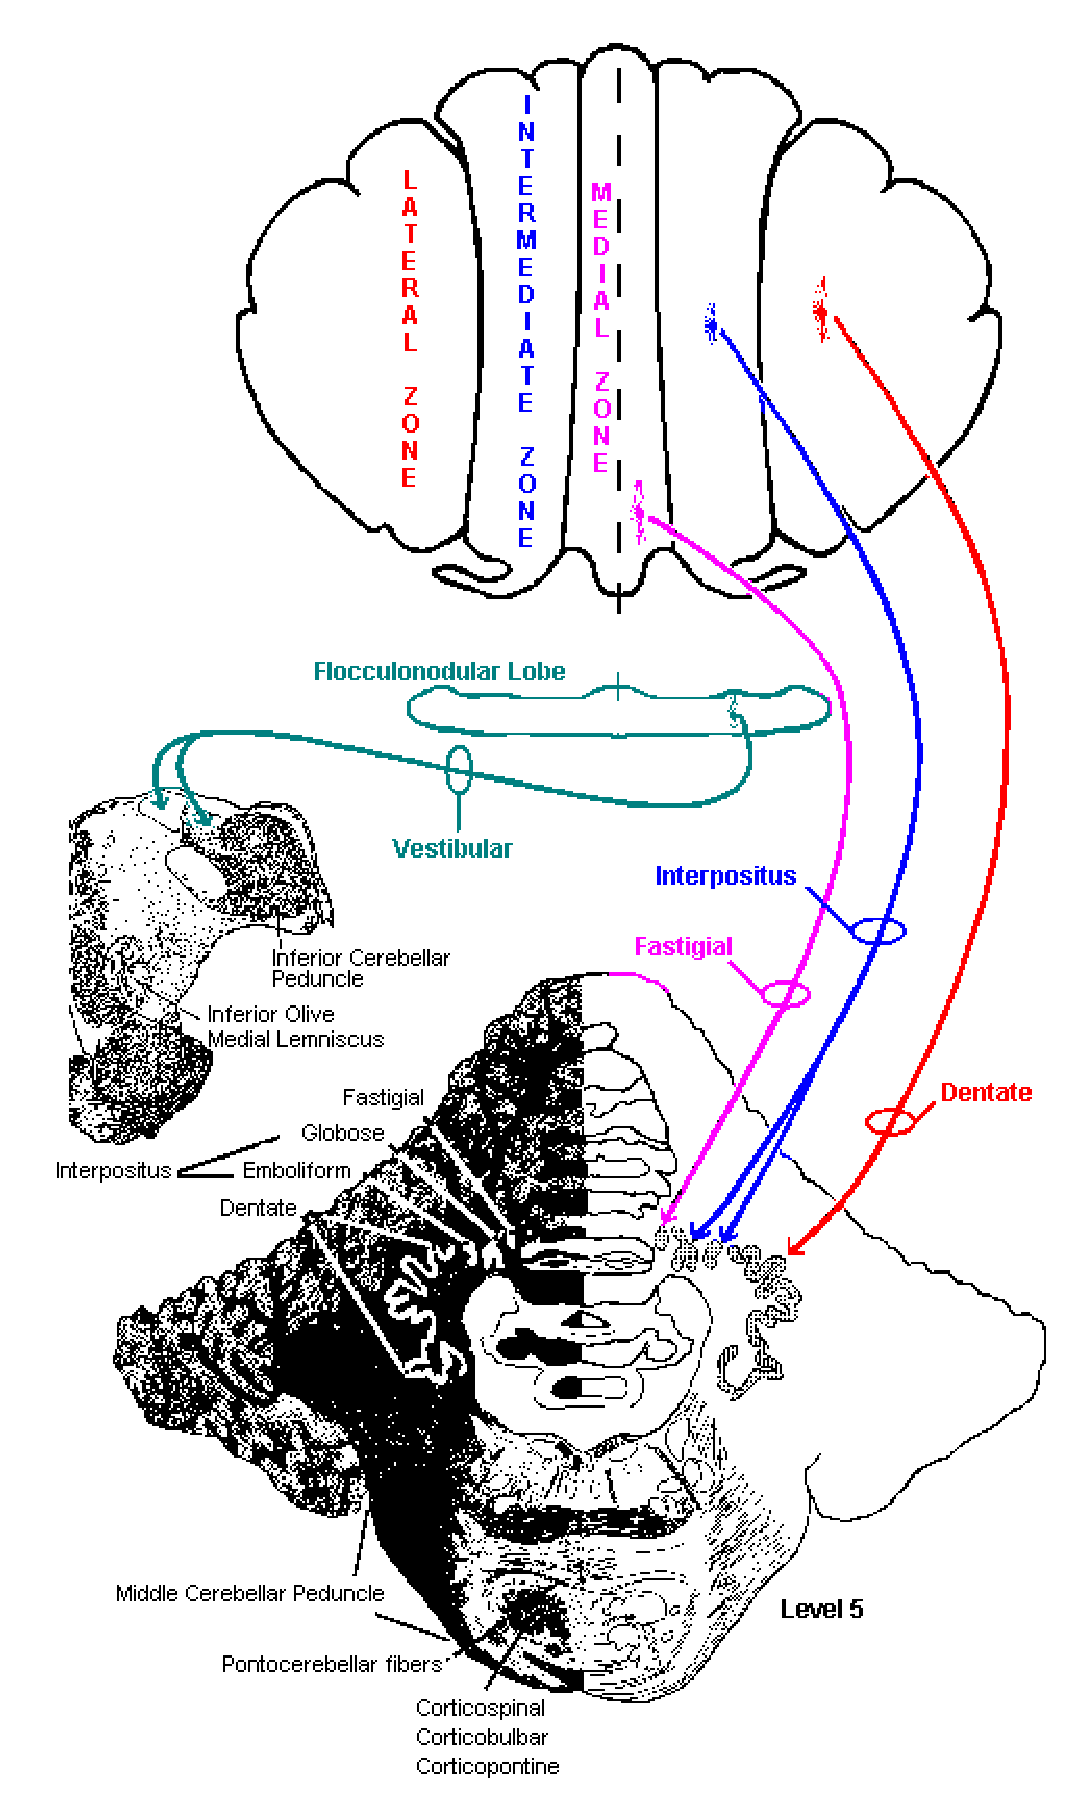
\includegraphics[height=8cm,
    angle=0]{./images/cereberrum_function_division.eps}  
    }
\caption{ (A) Major anatomical subdivisions of the cerebellum: Hemispere,
Vermis, Anterior lobe, Posterior lobe, Flocculonodular lobe, Primary fissure, Horizontal
fissure, Posterior fissure, Nodulus, Flocculus. (B) Functional
distinction is based on medial-to-lateral direction: Lateral zone,
Intermediate zone and Medial zone
\footnote{\url{http://www.neuroanatomy.wisc.edu/cere/text/P5/S/C44.htm}}}
\label{fig:cerebellum_anatomy}
\end{figure}

Like cerebrum, the cerebellum also contains the grey matter and white matter.
The grey matter has 2 disconnected parts: {\bf cerebellar cortex}
(Sect.\ref{sec:cerebellar_cortex}) and {\bf deep cerebellar nuclei} (or
cerebellar deep nuclei - Sect.\ref{sec:deep_cerebellar_nucle}).

\subsection{dentate nuclei of cerebellum}
\label{sec:dentate-nuclei-cerebellum}

These nuclei relay the information from the Purkinje cells to the thalamus,
which then projects to the cortex and the striatum.

\subsection{Cerebellar cortex}
\label{sec:cerebellar_cortex}

On the surface of the cerebellar cortex, the fissures divide the cerebellal
surface into different lobes, separated by the different fissure,
Fig.\ref{fig:cerebellum_anatomy}:
\begin{itemize}
  \item anterior lobe:
  \item posterior lobe: 
  \item flocculonodular lobe (vestibulocerebellum): regulate balance and eye
  movement
\end{itemize}
\textcolor{red}{These lobes divide the cerebellum in humans, top to
bottom (and in other animals: from rostral to caudal).} 
Interestingly, exclcuding the flocculonodular lobe, in terms of functionality
of the 3 lobes, the more important distinction is divided from medial-to-lateral
direction (i.e. left-to-right in human) with 3 regions,
Fig.\ref{fig:cerebellum_anatomy} (B).
\begin{itemize}
  \item Lateral zone: receive input from
  olivocerebellar and pontocerebellar fibers carrying planning information from
  the posterior parietal area; and output to the lateral nuclei (see below the
  nuclei information).
   
  \item Intermediate zone (globose and emboliform): receive input from
  olivocerebellar and pontocerebellar fibers carrying information from primary
   motor cortex AND from DSCT and CCT; and output to 
  interpositus nuclei.
  
  \item Medial zone
  \item Flocculonodular zone (flocculonodular lobe)
\end{itemize}
\label{sec:cerebellum_zones}
Purkinje cells (Sect.\ref{sec:Purkinjie_nerves}) in different zones project to
different deep cerebellar nuclei.
 
The gyri on the cerebellum is called {\bf folium} (pl: folia). The folium of the
grey matter has 3 distinct layers and different cell type distribution,
Fig.\ref{fig:cerebellum_greymatter}.

The different layers
\begin{enumerate}
  
  \item {\bf molecular layer} (external layer): a flattened dendritic trees of
  Purkinje cells (Sect.\ref{sec:Purkinjie_nerves}), neuroglia cells
  (Sect.\ref{sec:neuroglia-cell}), tiny cells like local plexus (small cells of
  molecular layer), basket cells (Sect.\ref{sec:basket-cell}), chandelier cells
  (Sect.\ref{sec:chandelier-cells}), all of which are inhibitory neurons.
  It also contains axon of granule cells from nuclear layer, axon of Golgi
  cells, and end of Tendril climbing fiber.

  \item {\bf Purkinje layer} (nuclear layer): contains cell bodies of Purkinje
  neurons and Bergmann glial cells. 
  %contains granule cells, dendrites of
  %Golgi cells, and the end of Moss fiber.
  
  \item (thick) {\bf granular layer} (bottom, nuclear layer): densely packed
  with granule cells, and interneurons (mainly Golgi cells, and some Lugaro
  cells + unipolar brush cells)
\end{enumerate}
\url{http://en.wikipedia.org/wiki/Cerebellum}
The axon of the Purkinje cells travels deep into the white matter to control the
deep cerebellum nuclei.

\begin{figure}[hbt]
  \centerline{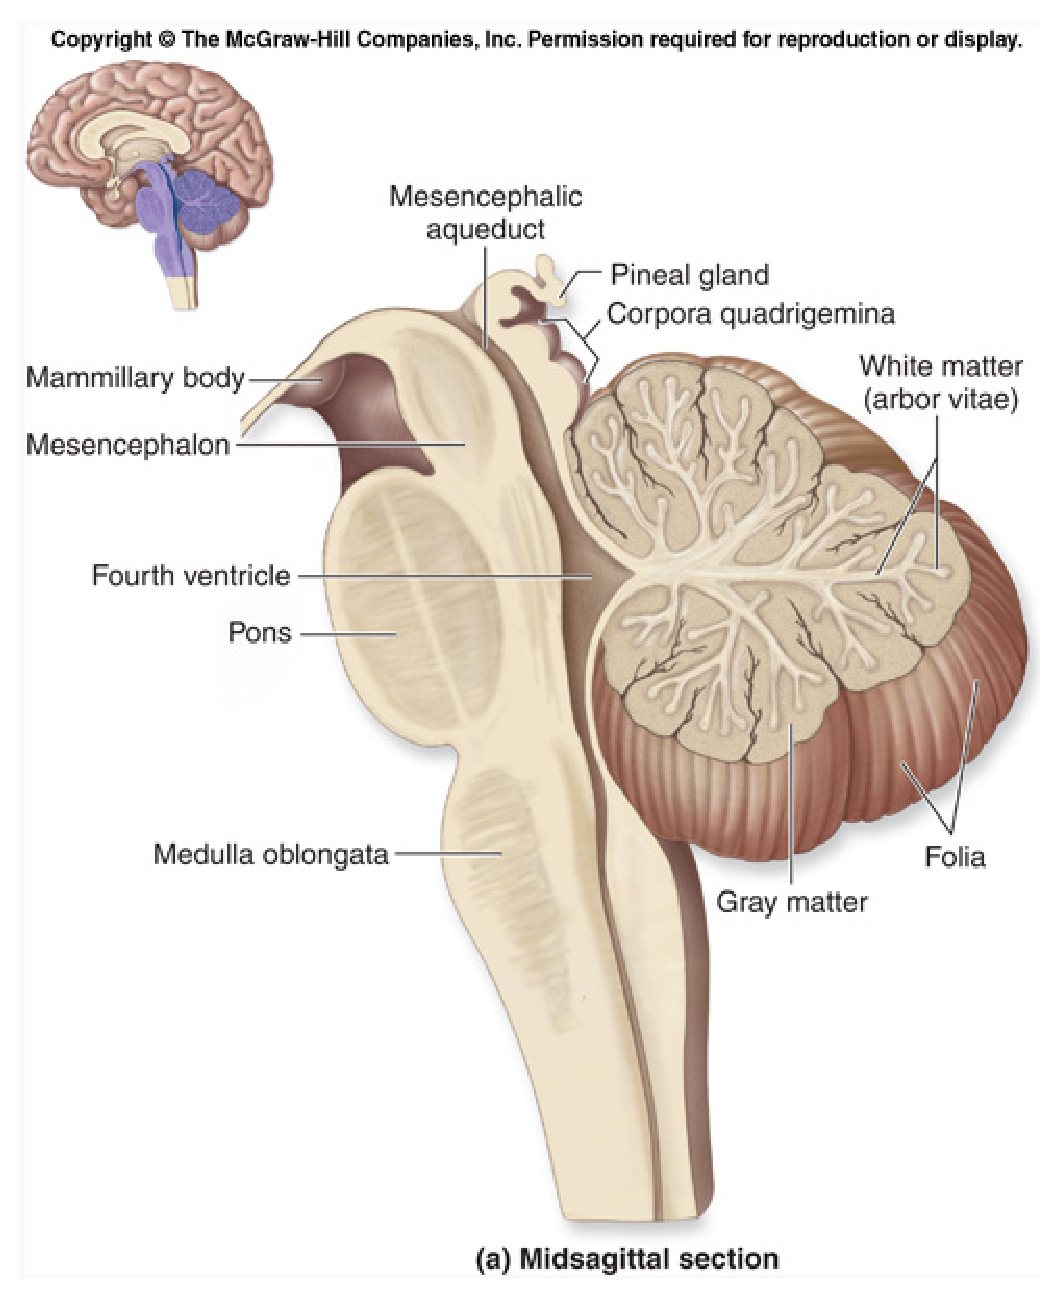
\includegraphics[height=8cm,
    angle=0]{./images/brain_10.eps},
    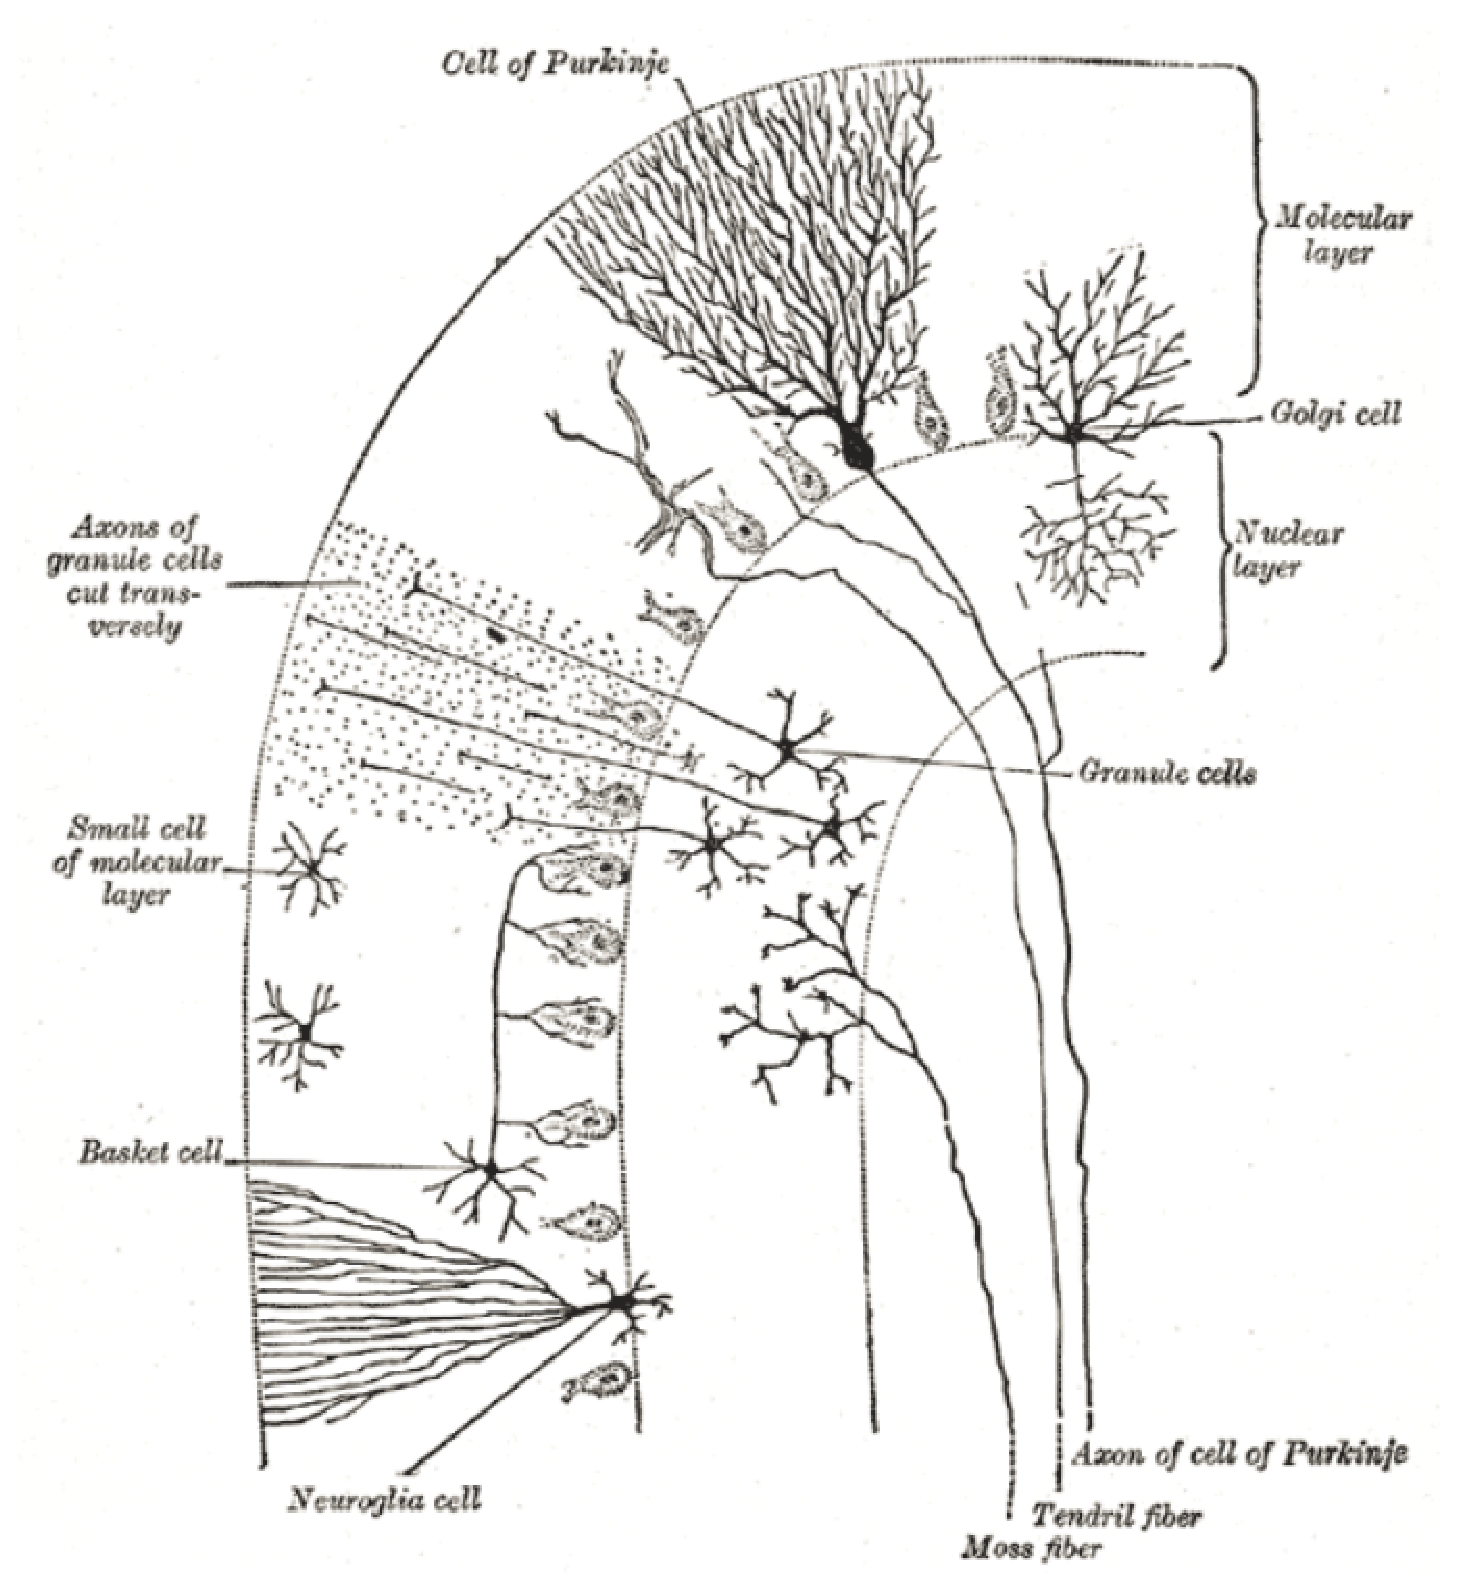
\includegraphics[height=8cm,
    angle=0]{./images/cerebellar-folium-neurons.eps}}
  \caption{Grey matter's layers in cerebellum
  \footnote{\url{http://en.wikipedia.org/wiki/Purkinje_cell}}. (B) Different
  cell types in a cerebellar folium}
\label{fig:cerebellum_greymatter}
\end{figure}

\subsection{Deep Cerebellar nuclei}
\label{sec:deep_cerebellar_nucle}

The grey matter of cerebellum has 4 cerebellar deep nuclei (embedded in the
white matter in the center):  
\url{http://www.neuroanatomy.wisc.edu/cere/text/P5/intro.htm}
\begin{itemize}
  \item denlate nuclei (most lateral deep cerebellar nuclei): receive input from
  lateral zone of the cerebellum 
  
  \item interpositus nuclei: receive input from intermediate zone of cerebellum
  
  \item fastigial nuclei (lie in the medial zone of the cerebellum): 
  
  \item vestibular nuclei : receive input from flocculonodular zone
\end{itemize}
Three nuclei receive inhibitory inputs (GABAergic)
from Purkinjie cells (Sect.\ref{sec:Purkinjie_nerves}), and excitatory input
from the collaterals of both mossy and climbing fibers as they pass through the
deep white matter on their way to the overlying cerebellar cortex.
The interplay of the inhibitory (Purkinje cell) and excitatory (mossy and
climbing fiber) inputs to the deep nuclei determines their output signal to the
other parts of the brain.

% Anatomically, cerebellum contains 2 major parts:
% \begin{itemize}
%   \item 4 cerebellar deep nuclei (embedded in the white matter in the center):
%   three nuclei receive inhibitory inputs (GABAergic) from Purkinjie cells
%   (Sect.\ref{sec:Purkinjie_nerves})
%   
%   \item cerebellar cortex
% \end{itemize}

{\bf Mammaliary bodies} are a pair of small round bodies, as part of the
diencephalon and part of the limbic system (Sect.\ref{sec:limbic-system}).
They have two groups of nuclei, the medial mammillary nuclei and the lateral
mammillary nuclei. They act as a relay for impulses coming from amygdala
(Sect.\ref{sec:amygdala}) and hippocampus (Sect.\ref{sec:hippocampus})
as part of the Papez circuit (Sect.\ref{sec:Papez_circuit}). 


\subsection{Cerebellal white matter}
\label{sec:cerebellal_whitematter}

The white matter has two parts:
\begin{itemize}
  \item internal: arbor vitae
  \item cerebellar peduncles: the part that connect cerebellum to the brain stem
  (Sect.\ref{sec:brain-stem}). There are totally 6 peduncles (3 on left and 3
  on right) 
  \begin{enumerate}
    \item superior cerebellar penduncle: the primary output of the cerebellum,
    i.e. mostly fibers carrying signals to midbrain
    
    \item middle cerebellar penduncle: carry input signals from contralateral
    cerebral cortex
    
    \item inferior cerebellar penduncle: receive proprioceptive (stimuli
    produced and perceived within an organism) signals from 
    ipsilateral side (i.e. the organ from the same side of the peduncle) of the
    body.
    
  \end{enumerate} 
\end{itemize}


\section{3. Brain stem}
\label{sec:brain-stem}

{\bf Brain stem} is the lower part of the brain, adjoining and structurally
continuous with the spinal cord. Brain stem, though small, play essential role
as the interface from the CNS to all parts of body.

The brain stem looks like a stalk supporting the cerebrum. It has 3
subdivisions (from top to bottom): midbrain, pons, and medulla oblongata (or
simply medulla), as shown in Fig.~\ref{fig:brain_stem}. The brain stem is involved in speech and
keeping the smooth connection from the CNS to other parts of the body.

\begin{figure}[hbt]
  \centerline{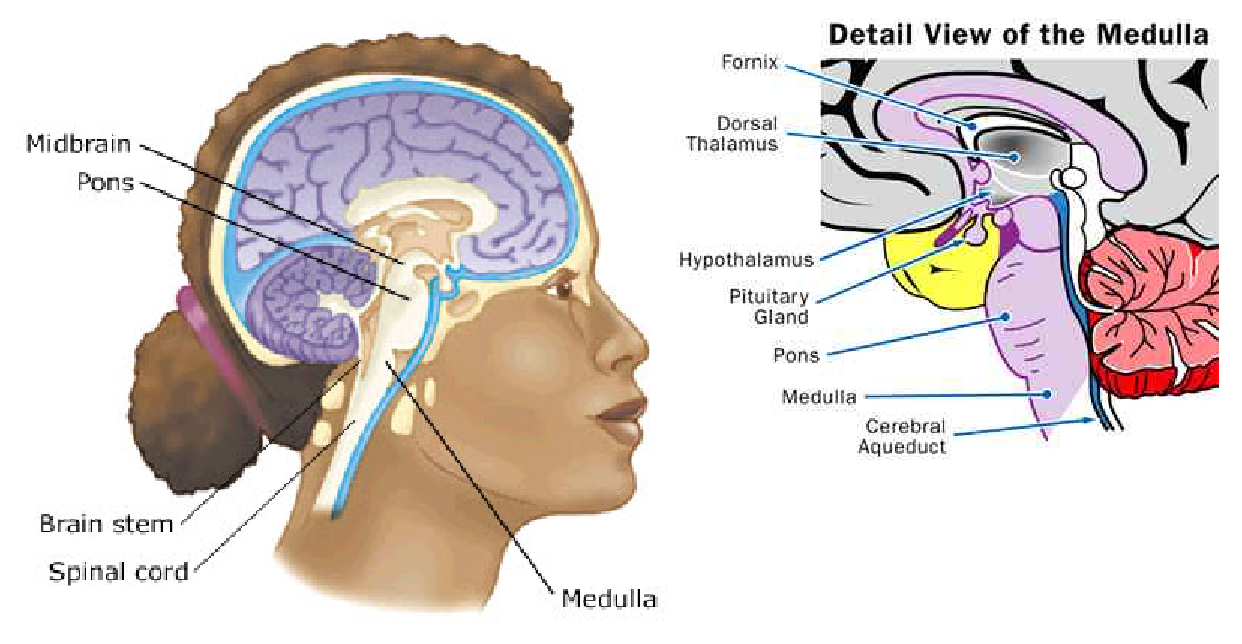
\includegraphics[height=5cm,
    angle=0]{./images/slice_brain.eps}}
\caption{(A) Brain stem; (B) detail of medulla}
\label{fig:brain_stem}
\end{figure}

\subsection{raphe nuclei (Greek: seam)}
\label{sec:raphe-nuclei}

The raphe nuclei (Greek: "seam") are a moderate-size cluster of nuclei
(Sect.\ref{sec:nuclei_structure}), as part of the reticular formation
(Sect.\ref{sec:reticular-formation}) and is found in the brain stem
(Sect.\ref{sec:brain-stem}).

The neurons in this nuclei synthesize serotonin (Sect.\ref{sec:serotonin}), and
thus, the main function is to release serotonin to the rest of the brain,
Fig.\ref{fig:serotonin-pathways}, and thus have a vast impact to CNS (to control
mood, memory processing, sleep, cognition). In the brain serotonin is produced
in the upper raphe nuclei and in the caudal raphe nuclei and then travels along
the serotonins pathway to other parts of the brain and spinal cord.

Serotonergic neurons are grouped in the brainstem: in the pons and in the cores
of the joint. For target locations, check
the brain-region distribution of the receptors -
Sect.\ref{sec:serotonin-receptors}.

The projection can be divided into 3 pathways:
\begin{enumerate}
  \item  {\bf Descending projections} go to the spinal cord from the bridge.
  
  This is known as {\bf caudal pathway} (from Raphe nuclei to medulla and spinal
  cord): Uses mainly 5HT1 receptors 'slow excitation' (some uses 5HT3 receptors
  in area postrema trigger vomiting), causes contraction or uterine muscles
  cramps; causes some contraction of blood vessel walls" blood pressure'; causes
  mild motor neuron excitation; stimulates release of endorphins that then
  inhibit pain messages;
  
  \item raphe nuclei neurons give {\bf ascending projection} to the cerebellum,
  to the limbic system, to basal ganglia, to cortex, i.e.
\begin{itemize}
  \item to NAc - Sect.\ref{sec:nucleus_accumbens}
  \item to striatum - Sect.\ref{sec:striatum}
  \item to all regions of the cortex, e.g. limbic system (a subdivision of the
  cortex - Sect.\ref{sec:limbic-system})
  \item to hippocampus
  \item to cerebellum
\end{itemize}

  \item At the same time, the neurons of the dorsal and medial raphe nuclei give
 axons, which differ morphologically electrophysiologically, target of innervation and
sensitivity to certain neurotoxic agents, such as, methamphetamine. 
\end{enumerate}

\begin{figure}[hbt]
  \centerline{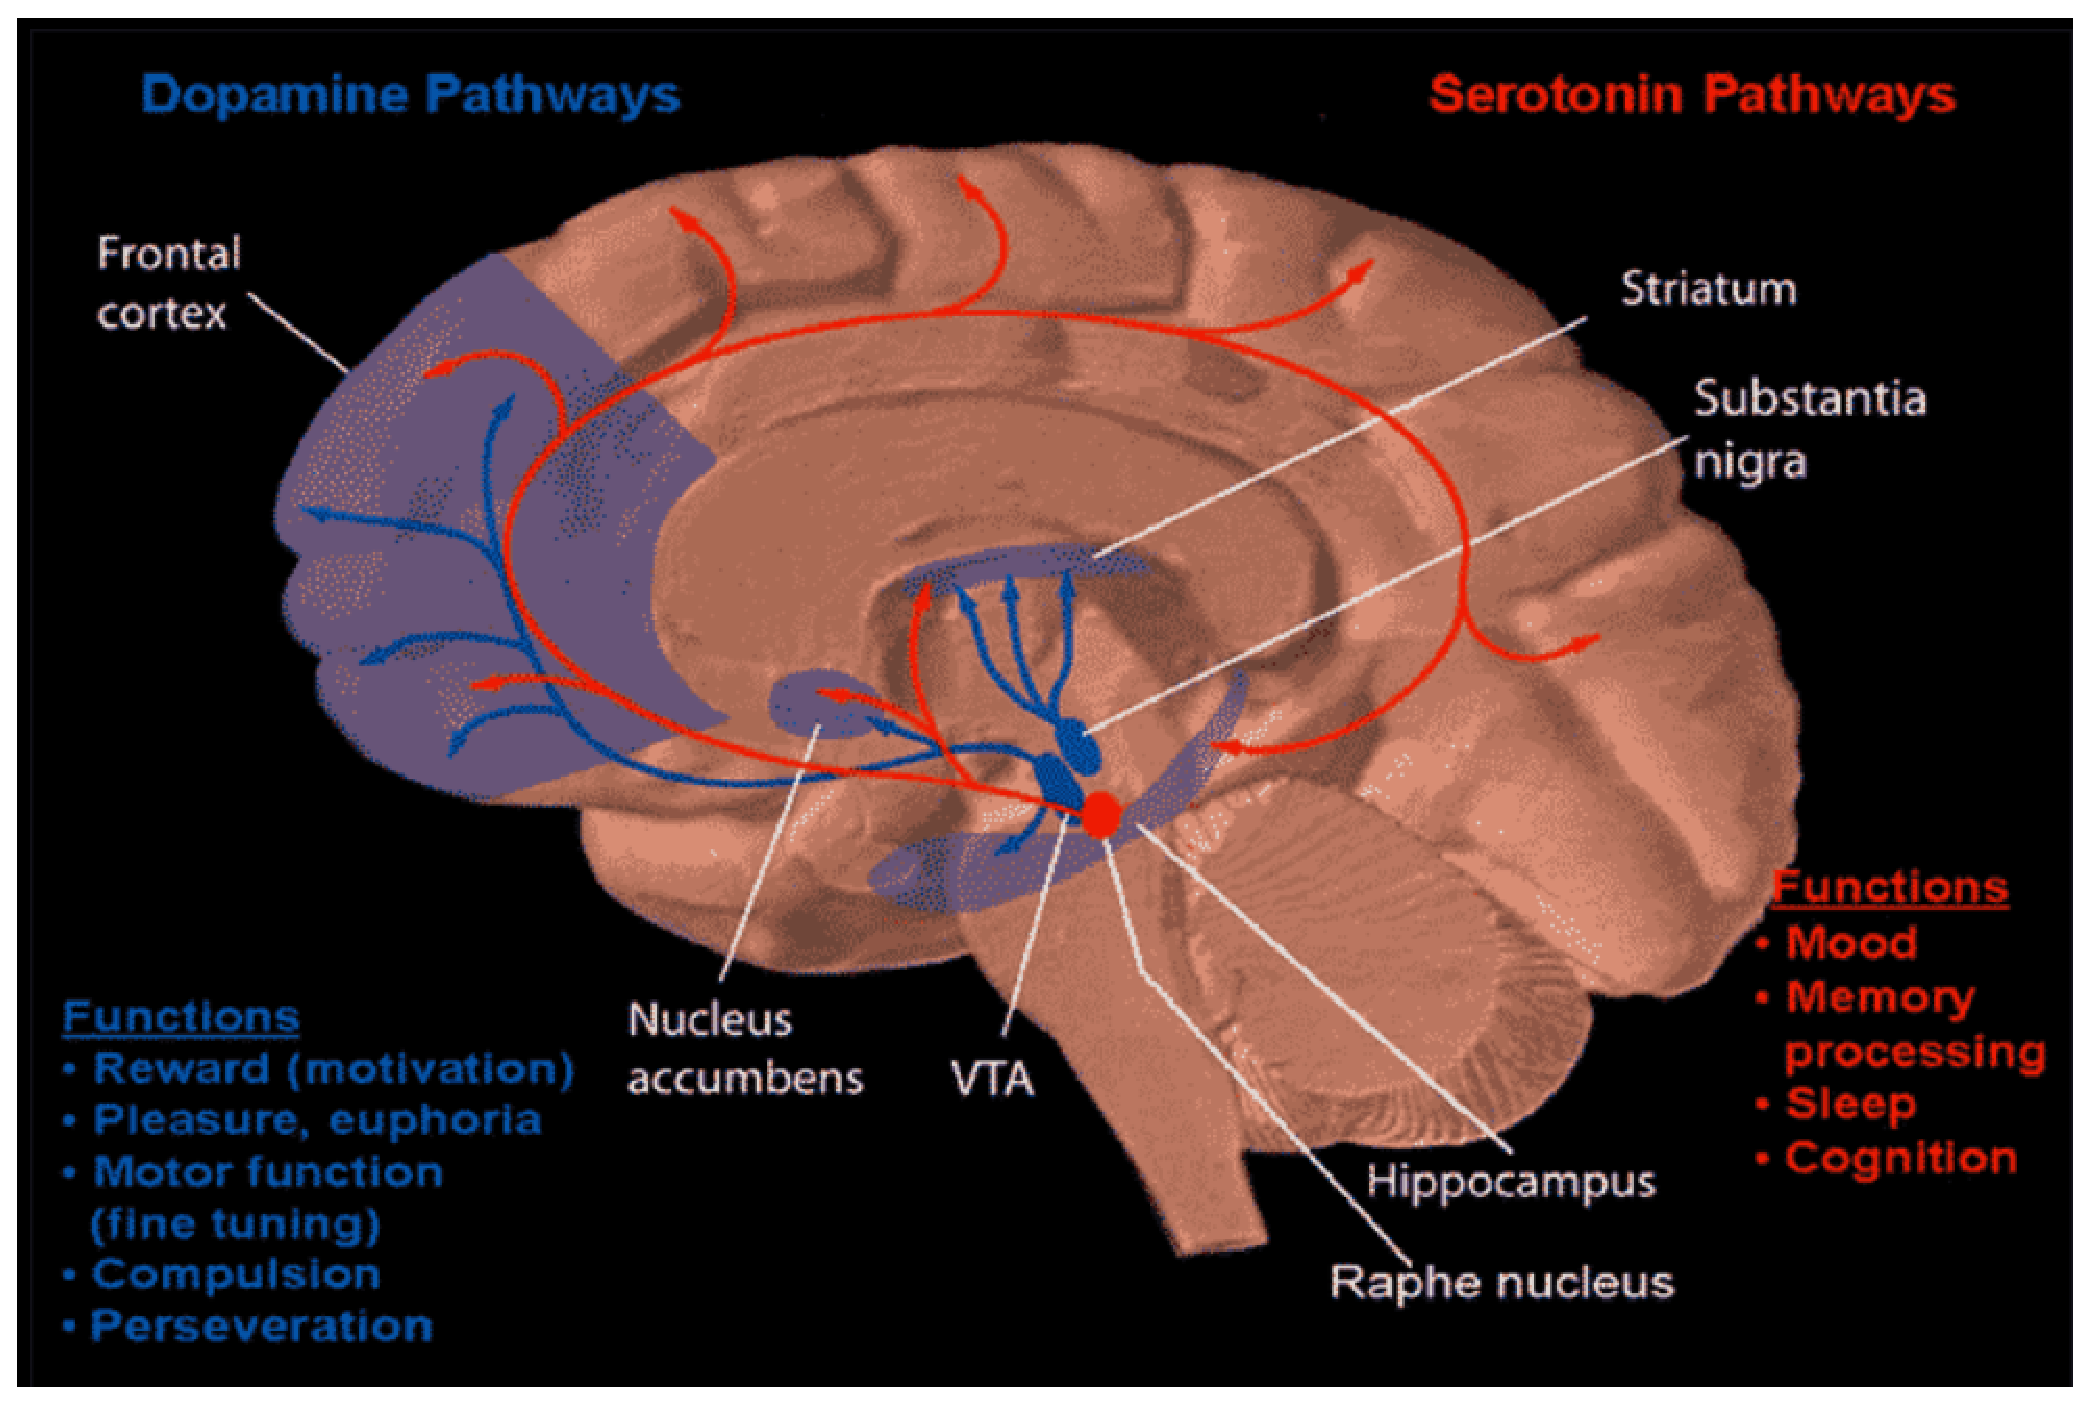
\includegraphics[height=5cm,
    angle=0]{./images/serotonin-pathways.eps}}
\caption{(Rostral raphe nuclei) serotonin pathways and Dopamine pathways. The
(Caudal raphe nuclei) serotonin pathway projects to spinal cord and medulla.
Serotonin is used throughout the body in multiple physiological roles, and just 2\% 
of serotonin used in CNS.}
\label{fig:serotonin-pathways}
\label{fig:dopamine-pathways}
\end{figure}


\subsection{Midbrain}
\label{sec:midbrain}

During embryonic stages, the {\bf midbrain} is developed from mesencephalon
vesicle (Greek: {\it mesos} = middle, {\it enkephalos} = brain) 

It is situated near the center part of the brain, i.e. locates just below the
cerebral cortex (Sect.\ref{sec:cerebral_cortex}), and above the pons
(Sect.\ref{sec:pons}) of the hindbrain.
It is the hub of vision, hearing, motor control, sleep/wake, arousal
(alertness), and temperature regulation.

The midbrain underneath the cerebral cortex and above the hindbrain
(Sect.\ref{sec:hindbrain}). In this region, the spinal cord and brain come
together to form the various functions of the midbrain.


The midbrain comprises %dorsal part (tectum) and ventral part (peduncle).
\begin{enumerate}
  
  \item dorsal (posterior) part: corpora quadrigemina (tectum, quadrigeminal
  plate (colliculi)) - Sect.\ref{sec:corpora-quadrigemina}

Tectum in non-mammal species (fish, birds) are large, but that in mammals
(especially primates) are smalled due to massive expansion of cerebral cortex;
and reduce the function to as the center for eye movement control.
  
  \item central part: tegmentum - Sect.\ref{sec:tegmentum}
  
  ascending and descending tracts, reticular nuclei, nuclear masses
  
  \item ventral (anterior) part: ventral tegmented area (VTA) -
  Sect.\ref{sec:ventral-tegmented-area}), cerebral peduncles -
  Sect.\ref{sec:cerebral-peduncles}
  
\end{enumerate}
% , {\bf
% tegmentum}, the cerebral aqueduct (or ventricular mesocoelia or "iter"), and the
% cerebral peduncles, as well as several nuclei and fasciculi.
References:
\begin{itemize}
  \item
  \url{http://www.slideshare.net/danielveladuartemd/the-anatomy-of-midbrain}
\end{itemize}

\begin{figure}[hbt]
  \centerline{
  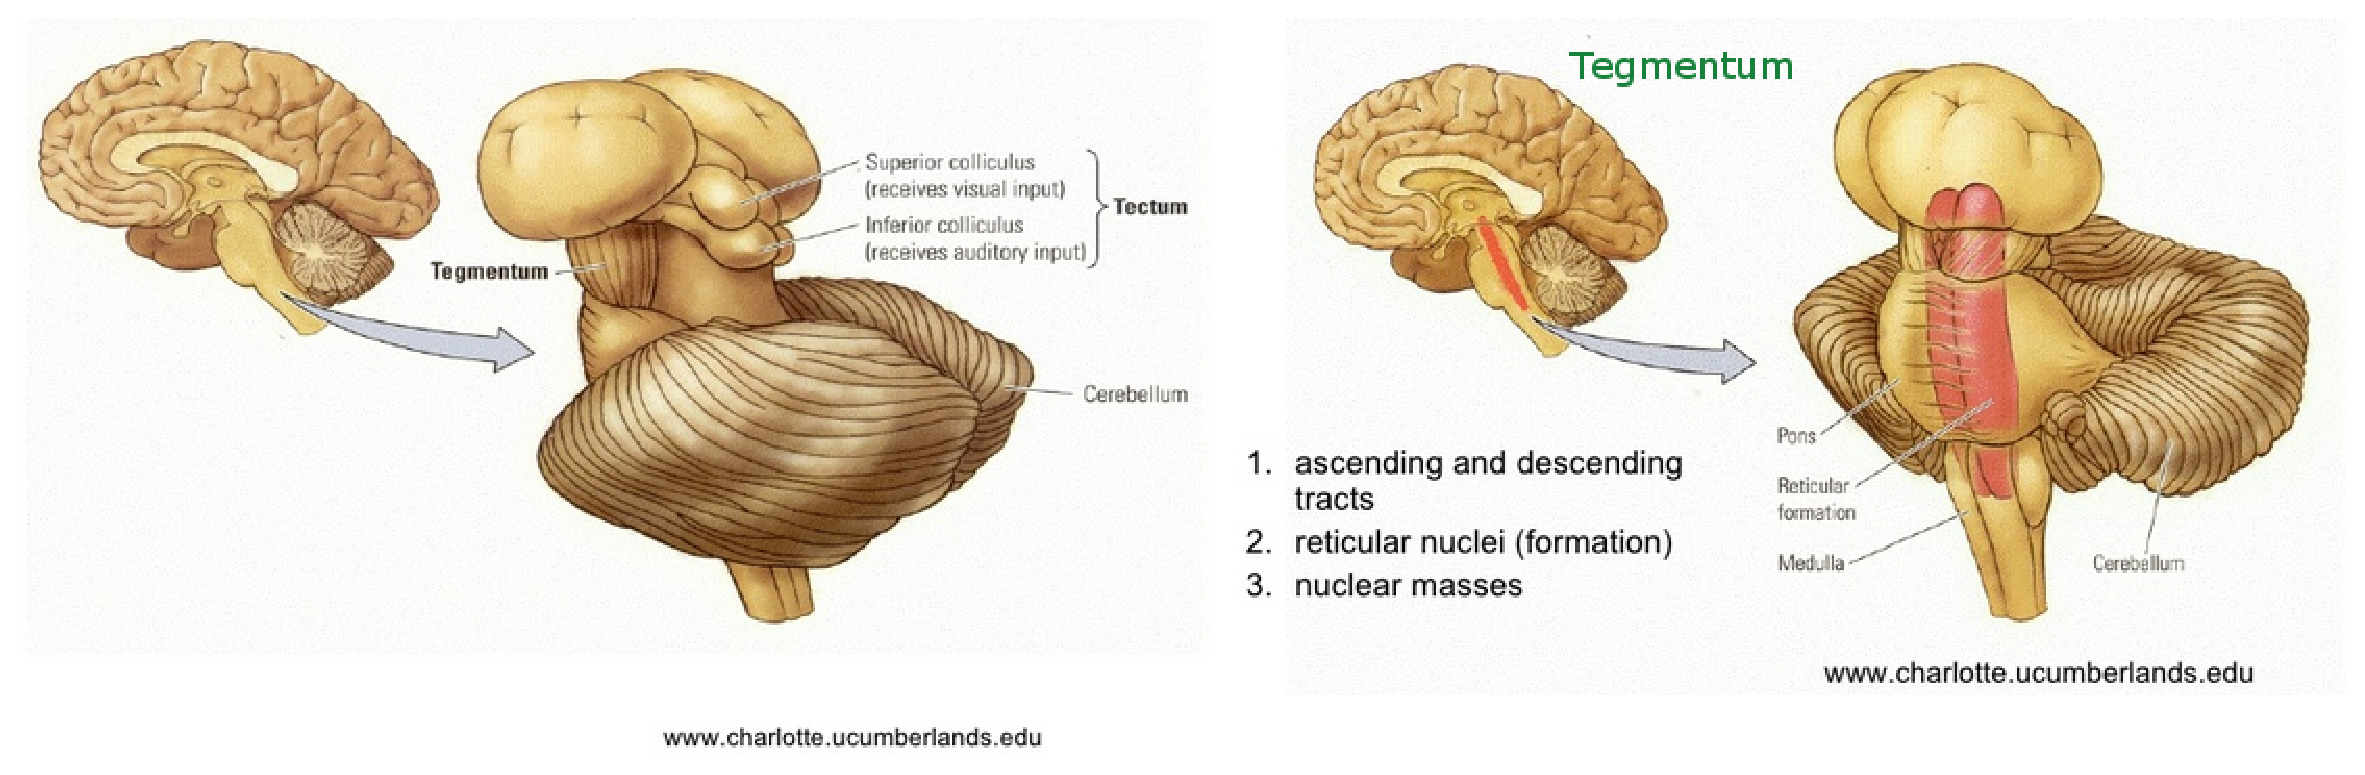
\includegraphics[height=5cm,
    angle=0]{./images/midbrain.eps}}
\caption{Midbrain: tectum, tegmentum}
\label{fig:midbrain}
\end{figure}

\subsection{-- dorsal (posterior) part: corpora quadrigemina (tectum,
quadrigeminal plate (colliculi))}
\label{sec:corpora-quadrigemina}
\label{sec:tectum}
\label{sec:inferior-colliculus}
\label{sec:superior-colliculus}

Greek: {\it tegos} = roof (any covered room of a house)

{\it corpora quadrigemina} of tectum (aka 4 bodies of the roof midbrain) is the
collective name for both inferior colliculus (rostral part or lower midbrain)
and superior colliculus (caudal part or upper midbrain): both located in the
dorsal part of the midbrain.


\begin{enumerate}
  
  \item {\bf inferior colliculus (IC)} nucleus (one on each side of the
  midbrain) (Latin =  lower hill):   principal midbrain nucleus of the auditory
  pathway; with 3 subdivisions (central nuclelus, central cortex, and external cortex)
  
  This is the place where vertically orienting data (from fusiform cells in
  dorsal cochlear nucleus) synapse with horizontally orienting data, i.e.
  the sound data are fully integrated.

\begin{verbatim}
input: from  several peripheral brainstem nuclei in the auditory pathway, as
       well as inputs from the auditory cortex
\end{verbatim}  

  \item {\bf superior colliculus} (optic tectum, tectum) (a pair of structures
  with one on each side of the midbrain, and sit belows the thalamus
  (Sect.\ref{sec:thalamus}), and surrounded by pineal gland):  the visual
  processing centers

NOTE: \textcolor{red}{the microstructure of the tectum varies across species}.
It is a layered structure, with a number of layers that varies by species.
In frogs, it has 4 layers; as known in a study by Lettvin et al.
(Sect.\ref{sec:Lettvin-what-the-frog-eye}).


In mammals, there are 7 layers
\begin{itemize}
  \item superficial layers: 
  
  INPUT: receive input mainly from (1) retina, (2) vision-related
  areas of the cerebral cortex (primary visual cortex (area 17), (3) secondary
  visual cortex (area 18, area 19), and (4) two tectal-related structures called
  the pretectum and parabigeminal nucleus.
  
  OUTPUT: (1) one of the most important outputs goes to  pulvinar and lateral
  intermediate areas of the thalamus (which in turns direct to areas in the
  cerebral cortex that are involved in controlling the eye movement); then
  (2) output to the pretectal nuclei, lateral geniculate nucleus of the
  thalamus, and the parabigeminal nucleus
  
\begin{enumerate}
  \item Lamina I (SZ, stratum zonale):
  
  \item Lamina II (SGS, stratum griseum superficiale)
  
  \item Lamina III (SO, stratum opticum)
\end{enumerate}
  
  \item intermediate layers: 

INPUT: see box

OUTPUT: 

\begin{enumerate}
  \item Lamina IV (SGI, stratum griseum intermedium)
  
  \item Lamina V (SAI, stratum album intermedium)
\end{enumerate}

  \item deep layers

INPUT: see box

OUTPUT: two large descending pathways: (1) to brainstem, (2) to spinal cord;
and many others ascending projections to different sensory and motor centers.

\begin{enumerate}
  \item Lamina VI (SGP, stratum griseum profundum)
  \item Lamina VII (SAP, stratum album profundum)
\end{enumerate}
\end{itemize}
NOTE: intermediate layers and deep layers receive inputs from a very diverse set
of sensory and motor structures (\textcolor{red}{most areas in the cerebral cortex
projects to these layers}, projection from (substantia nigra, para
reticulata) via inhibitory neurotransmitters GABA; and somatosensory inputs
from the face via spinal trigeminal nuclelus -
Sect.\ref{sec:trigeminal-nerve};  as well as inputs from the hypothalamus,
zona incerta, thalamus, and inferior colliculus)

\end{enumerate}

\subsection{-- central part: tegmentum}
\label{sec:tegmentum}

{\bf Tegmentum} is the central part of the midbrain, Fig.\ref{fig:midbrain},
extending from the substantia nigra (Sect.\ref{sec:substantia_nigra}) to the cerebral
aqueduct, forming the floor of the midbrain that surrounds the cerebral aqueduct
(Sect.\ref{sec:cerebral_aqueduct}).

\subsection{-- ventral (anterior) part: ventral tegmented area (VTA), cerebral
peduncles} 

% - Sect.\ref{sec:cerebral-peduncles}
% Sect.\ref{sec:ventral-tegmented-area}), 
  
\subsection{ventral tegmented area (VTA)}
\label{sec:ventral-tegmented-area}

{\bf Ventral tegmented area} (VTA,  ventral tegmental area of Tsai, or ventral
tegmentum) is a part of the basal ganglia (Sect.\ref{sec:basal-ganglia}) in the
midbrain (Sect.\ref{sec:midbrain}). VTA is a group of neurons (called A10)
located close to the midline on the floor of the midbrain.

Originally, VTA is considered as a nucleus (Sect.\ref{sec:nuclei_structure}),
but nowadays it is refered to as an area due to the heterogeneous
cytoarchitecture features
\begin{itemize}
  \item originally: Oades (1987) identified four primary nuclei: 
  nucleus paranigralis (Npn), the nucleus parabrachialis pigmentosus (Npbp), the
  nucleus interfascicularis (Nif), and the nucleus linearis (Nln) caudalis and rostralis
  
  \item presently: 4 zones:
  paranigral nucleus (PN), the parabrachial pigmented area (PBP), the
  parafasciculus retroflexus area (PFR), and the ventral tegmental tail (VTT)
  
  \textcolor{red}{The PN and PBP are rich in  dopamine-synthesizing neurons},
  whereas the other two regions have low densities of these neurons.
  Recent studies shows the number of doparminergic neurons is about 50-60\% of
  all neurons in VTA \citep{margolis2006}; a slower number than previously
  estimated 77\% \citep{johnson1992}.

  The tail of the VTA (tVTA) - a functionally distinct brain structure -  has a
sizable population of GABAergic neurons (Sect.\ref{sec:GABAergic-neurons}).
These neurons has been shown to have a large network of GABAergic neurons that
are interconnected via gap junctions (Sect.\ref{sec:gap-junction}). This network
allows for electrical conduction, which is considerably faster than the chemical
conduction of signals between synapses.

  The VTA also contains a small percentage of excitatory glutamatergic neurons;
  yet this number increases signficantly in primates compared to other mammals.
  VTA of the mouse contains approximately 25,000 neurons, while the VTA of a
  33-year-old man contains around 450,000 cell bodies.
\end{itemize}


Neurons in VTA produces dopamine (Sect.\ref{sec:dopamine}), and these neurons 
project to numerous areas of the brain, with 2 primary efferent projects:
(1) {\bf prefrontal cortex (PFC)}, (2) {\bf nuclelus accumbens}. 
\begin{itemize}
  \item {\bf mesocortical pathways} (Sect.\ref{sec:mesocortical-pathway}): VTA
  $\rightarrow$ PFC
  
  
  \item {\bf mesolimbic pathways} (Sect.\ref{sec:mesolimbic-pathway}): VTA
  $\rightarrow$ nucleus accumbens (Sect.\ref{sec:nucleus_accumbens})
\end{itemize}
The complete lists of dopaminergic projections from VTA are found in
Sect.\ref{sec:dopaminegic_pathways}

\subsubsection{cerebral peduncles}
\label{sec:cerebral-peduncles}

{\bf Cerebral peduncles} has 3 parts:
\begin{enumerate}
  \item  corticopontine fibers (frontopontine projection), 
  medial 5th: motor fibers from the precentral gyrus (motor strip)
  to the nuclei of cranial nerves V (trigeminal), VII (facial), and XII
  (hypoglossal)
  
  \item corticospinal fibers (middle 3/5th):
  somatotopically distribution: arm (medial), leg (lateral, trun in between)
   
  
  \item temporopontine  fibers (latheral 5th): originate from the temporal lobe
  and end in nuclei pontis
 
\end{enumerate}


\subsubsection{Cerebral aqueduct}
\label{sec:cerebral_aqueduct}
{\bf Cerebral aqueduct} (aqueductus mesencephali, mesencephalic duct, or the
aqueduct of Sylvius): locates within the midbrain. 
It locates dorsal to the pons and ventral to the cerebellum.

Its function is to connect the third ventricle in the diencephalon to the fourth
ventricle (Sect.\ref{sec:ventricle_brain}).

    


\subsection{Pons}
\label{sec:pons}

The {\bf pons} (about 2.5cm in length) is part of the hindbrain
(Sect.\ref{sec:hindbrain}). It is grown out of the metencephalon - the
cerebelum also grows out of this vesicle. So, there is only one way the
cerebellum can connect to the brain, i.e. via the pons.

There are two parts
\begin{enumerate}

  \item dorsal pons ({\bf pontine tegmentum}):  contains nuclei of 
  \begin{itemize}
     \item the cranial nerves: (trigeminal (5th), abducens (6th), facial (7th),
    and vestibulocochlear (8th) cranial nerve nuclei) and their 
    associated fibre tracts, the pontine reticular formation. 
  
     \item the {\it mesopontine cholinergic system} (containing 2cholinergic
     nuclei that project widely throughout the brain): the pedunculopontine
     nucleus (PPN) and the laterodorsal tegmental nucleus (LTN).
     \begin{itemize}
       \item PPN:  including arousal, attention, learning, reward, and voluntary
       limb movements and locomotion, (recently discovered) providing sensory
       feedback to the cerebral cortex \citep{tsang2010}.
       PPN is involved in the planning of movement (different
       networks of neurons in the PPN are switched on during real and imagined
       movement).
       PPN generate and maintains REM sleep (Sect.\ref{sec:REM_sleep}).
       
       
       \item LTN: 
     \end{itemize}
  
     \item the respiritory centres (two): the pneumotaxic centre and the
     apneustic centre.
     
  \end{itemize}

With different nuclei within, pontine tegmentum is a region associated with a
range of functions including sensory and motor functions (due to the cranial
nuclei and fiber tracts), control of stages of sleep and levels of arousal and
vigilance (due to the ascending cholinergic systems), and some aspects of
respiratory control
\url{https://en.wikipedia.org/wiki/Pontine_tegmentum}
  
  \item ventral pons ({\bf basilar part of the pons}): contains (1) the
  corticospinal tract running craniocaudally and can be considered the rostral
  extension of the ventral medulla oblongata; (2)
  additional transverse pontine fibres that continue laterally to
  become the {\it middle cerebellar peduncle} 
  
\end{enumerate}
 
The pons includes tracts that conduct signals from the brain down to the
cerebellum and medulla, and tracts that carry the sensory signals up into the
thalamus.

The pons is a large mass of fibre (white matter), is superior to the medulla
(Sect.\ref{sec:medulla_oblongata}).
The pons contains nuclei (Sect.\ref{sec:nuclei_structure}) that relay signals
from the forebrain to the cerebellum, along with nuclei that deal primarily with
sleep, respiration, swallowing, bladder control, hearing, equilibrium, taste,
eye movement, facial expressions, facial sensation, and posture.

\subsection{reticular formation (reticulum = little net)}
\label{sec:reticular-formation}

The {\bf reticular formation} is part of myelencephalon
(Sect.\ref{sec:myelencephalon}).  It is a set of interconnected nuclei; but not
anatomically well-defined, as the neurons involved are from different parts of
the brain (has many sensory afferent fibers that bring sensations and afferent
fibers from higher centers to lower centers). Because of that, it is a complex
network of about 100 tiny nuclei that occupies the central core of the brain
stem from the posterior boundary of the myelencephalon to the anterior boundary
of the midbrain. It is so named because of its netlike appearance
(\textcolor{red}{reticulum means "little net"}).

\begin{mdframed}
The reticular formation is quite interesting from psychological perspective, as
the various nuclei involved into a variety of functions, including
\textcolor{blue}{sleep, attention (definitely important for language), movement,
the maintenance of muscle tone, and various cardiac, circulatory, and
respiratory reflexes}. Generally, the myelencephalon does NOT play an important
role in language production or comprehension.

\begin{itemize}
  \item rostral part: modulatory function
  
  \item caudal part: premotor functions
\end{itemize}
\end{mdframed}

Although its boundries are not clear and it is present mainly in the
brainstem, its nuclei can be divided into three columns that are:

\begin{enumerate}
  \item  {\bf raphe nuclei} (median) - Sect.\ref{sec:raphe-nuclei}: where {\it
  serotonin} neurotransmitters are synathesized (Sect.\ref{sec:serotonin})
  
  \item {\bf magnocellular red nucleus} (medial zone): containing magnocellular
  cell (M-cell, large-size)  - Sect.\ref{sec:magn-neur-cells}
%   - this maps to medial geniculate nucleus in the thalamus
%   (Sect.\ref{sec:thalamus})
  
  
  \item {\bf parvocellular reticular nucleus} (lateral zone): 
%   this maps to lateral
%   geniculate nucleus  in the thalamus
  
\end{enumerate}
The medial reticular formation and lateral reticular formation are two columns
of neuronal nuclei with ill-defined boundaries, so they shares the cells with
medial geniculate nucleus and lateral geniculate nucleus in the thalamus
(Sect.\ref{sec:thalamus}).

\textcolor{red}{Input pathways}:
the afferent sensory action potentials travel through a web of neural networks,
got delivered into 
the reticular activating system (RAS), the "port-of-entry" into the brain.

\subsection{-- (ascending) reticular activating system (RAS)}
\label{sec:reticular-activating-system}

The ascending reticular activating system (ARAS), also known as the
extrathalamic control modulatory system or simply the reticular activating
system (RAS), is a set of connected nuclei in the brains of vertebrates
(connecting the brainstem to the cortex) that is responsible for regulating
wakefulness and sleep-wake transitions.  These pathways originate in the upper
brainstem reticular core and project through synaptic relays in the rostral
intralaminar and thalamic nuclei to the cerebral cortex. 

RAS's function is to prevent information overload by acting as a preliminary,
coarse sieve, a filter that serves to avoid overburdening the brain with
extraneous data. In other words, RAS decides what is important, and what can be
ignored by the brain. Typically, RAS responds to
\begin{enumerate}
  \item {\bf novelty}
  
You notice anything    new and different. For leadership purposes, this includes
anything out of the ordinary in day-to-day activities within your organization,
attending to changes in your employees relative to production, mood, and
interactions with others.

  \item {\bf For survival's sake, your RAS responds to:    your name, anything
  that threatens your survival,    and information that you need immediately.}
  
\end{enumerate}

The reticular activating system (RAS) is the portal through which nearly all
information enters the brain (except the smell - which is handled by olfactory
bulb - Sect.\ref{sec:olfactory-bulb}).

The reticular activating system (RAS) is a network of neurons located in the
brain stem that project anteriorly to the hypothalamus to mediate behavior, as
well as both posteriorly to the thalamus and directly to the cortex for
activation of awake, desynchronized cortical EEG patterns.   


{\bf The neuronal circuits of the RAS} are modulated by complex interactions
between a few main neurotransmitters. The RAS contains both cholinergic and
adrenergic components, which exhibit synergistic as well as competitive actions
to regulate thalamocortical activity and the corresponding behavioral state.


\subsection{Medulla (Medulla oblongata)}
%\label{sec:medulla}
\label{sec:medulla_oblongata}

The {\bf medulla oblongata} (or just medulla), is a major part of the
myelencephalon (Sect.\ref{sec:myelencephalon}), found in the lower portion of
the pons. By receiving inputs from the autonomic nervous system
(Sect.\ref{sec:autonomic_nervous_system}) - especially parasympathetic nervous
system, neurons cells in the medulla controls heart beat, blood pressure and
respiration. The neurons here projects to vagus nerve (X cranial nerve -
Sect.\ref{sec:vagus-nerve}).

Nucleus in the medulla oblongata
\begin{enumerate}
  \item inferior olivary nucleus - Sect.\ref{sec:inferior-olive-nucleus}
\end{enumerate}


\subsection{-- inferior olivary nucleus (inferior olive, IO)}
\label{sec:inferior-olive-nucleus}

The inferior olivary nucleus in the nucleus in the medulla oblongata -
Sect.\ref{sec:medulla_oblongata}. It is located in the ventral brainstem, gives
rise to the climbing fibers (CFs). The inferior olivary nucleus provides one of
the two main inputs to the cerebellum: the so-called climbing fibers, i.e. the
axon of the neurons in inferior olive
(IO) (Sect.\ref{sec:Inferior-Olive-neurons}).
Each climbing fiber winds closely around the dendrites of its corresponding
Purkinje cell, so that the activation of this fibre will cause a massive
excitation of this cell.
The axons of the Purkinje cells synapse on the neurons of the dentate nuclei of
the cerebellum, Fig.\ref{fig:cerebellum_position}(A).

Because of this, the IO plays a vital role in the functioning of cerebellum
(Sect.\ref{sec:cerebellum}). The inferior olive (IO) IO integrates the motor
task, i.e. information from the muscle proprioceptors. IO lesions or otherwise
disrupted connectivity between the cerebellum and the IO lead to motor problems
such as nystagmus, ataxia and dystonia.



% \begin{figure}[hbt]
%   \centerline{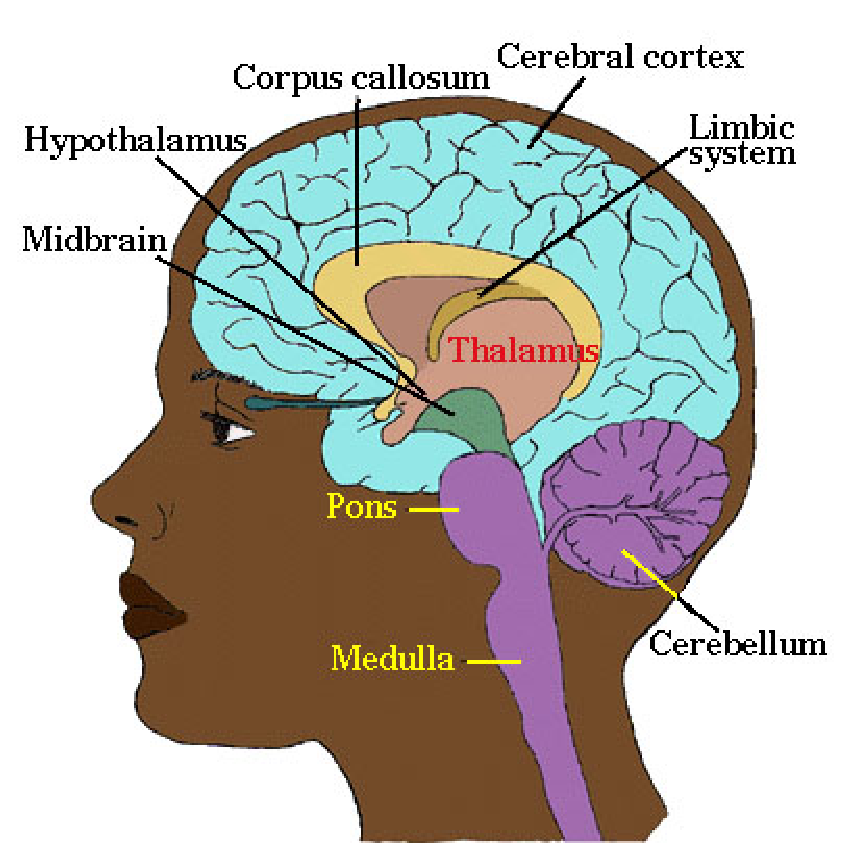
\includegraphics[height=5cm,
%     angle=0]{./images/brain_detail.eps}}
% \caption{Detail of different parts of the brain}
% \label{fig:brain_detail}
% \end{figure}

\section{Clearance of substances from brain}
\label{sec:clearance-in-brain}

From animal studies it is known that molecules contained in the interstitial
fluid (ISF) are cleared from the brain via different pathways.

\begin{enumerate}
  \item  ISF of white matter seems to be preferentially drained into
the cerebrospinal fluid (CSF) directly

  \item ISF of gray matter appears to flow outward via perivascular
spaces located alongside cerebral vessels and empty into cervical lymph nodes.

This drainage pathway could be impaired in late-onset AD due to impaired
pulsatility of cerebral vessels - Sect.\ref{sec:Alzheimer-hypothesis-impaired-clearance-Ab}

\end{enumerate}


\begin{verbatim}
7. Iliff, J. J. et al. A paravascular pathway facilitates CSF flow through the brain parenchyma and the clearance of interstitial solutes,
including amyloid beta. Science translational medicine 4, 147ra111 (2012).
8. Weller, R. O. Pathology of cerebrospinal fluid and interstitial fluid of the CNS: significance for Alzheimer disease, prion disorders
and multiple sclerosis. Journal of neuropathology and experimental neurology 57, 885–894 (1998).
9. Carare, R. O. et al. Solutes, but not cells, drain from the brain parenchyma along basement membranes of capillaries and arteries:
significance for cerebral amyloid angiopathy and neuroimmunology. Neuropathology and applied neurobiology 34, 131–144 (2008).
10. Szentistvanyi, I., Patlak, C. S., Ellis, R. A. & Cserr, H. F. Drainage of interstitial fluid from different regions of rat brain. The American
journal of physiology 246, F835–844 (1984).
11. Zhang, E. T., Richards, H. K., Kida, S. & Weller, R. O. Directional and compartmentalised drainage of interstitial fluid and
cerebrospinal fluid from the rat brain. Acta Neuropathol 83, 233–239 (1992).
\end{verbatim}

\chapter{Brain evolution}
\label{chap:brain-evolution}

All the organisms exist in the world have been classified into six Kingdoms;
namely, Bacteria, Archaea, Protista, Plantae, Fungi, and Animalia. Protozoa and
metazoa are two subgroups under Kingdom Protista and Kingdom Animalia respectively.
In the early classifications, the unicellular protozoans were considered as
simple animals. However, now they are put into diverse and large Kingdom Protista.
Protozoans live either singly or in colonies. They are considered as unicellular
organisms. Therefore, they do not contain any tissue or organs, which are
defined as a collection of differentiated cells with a definite function. 

Simple nerve nets seen in animals like {\it cnidaria} evolved first, followed by
nerve cords in bilateral animals  -  ventral nerve cords in invertebrates and
dorsal nerve cords supported by a notochord in chordates. Bilateralization led
to the evolution of brains, a process called cephalization.

The term ``cerebral ganglion" be used instead of ``brain'' when referring to
primitive bilateran animals, e.g. acoelomate worm
(Sect.\ref{sec:acoelomate-worm-brain}).

The path from a few cells to a full brain has taken hundreds of millions of
years in evolutionary time. But during embryonic development, the elaborate
process takes just days or months (Sect.\ref{sec:brain_development}).  
\begin{itemize}
  \item
  \url{https://www.scientificamerican.com/article/worm-discovery-brain-evolution/}
  
Researchers find a genetic link between the human brain and a sea-dwelling worm


  \item \url{http://bio.sunyorange.edu/updated2/comparative_anatomy/anat.html2/N_SPINAL.htm}
  \item 
\end{itemize}


\section{Non-brain organisms}

\section{-- Protozoans}
\label{sec:protozoans}

Protozoans are usually microscopic and show an extraordinary diversity in shape,
structure, symmetry and adaptations to numerous environments.

Protozoans can be classified into several subgroups mainly based on their
morphology, namely; Flagelletes, Amoeboids, Sporozoans, and Ciliates.  However,
their classification has been a problematic area of taxonomy.

It is believed that protozoans have evolved before metazoans
(Sect.\ref{sec:metazoan-brain}).
Protozoans have organelles, which are functionally equivalent to tissues or
organ systems in metazoans. Organelles are located inside the cell of
protozoans.

\subsection{Single-celled eukaryote}
\label{sec:single-celled-eukaryote}

Action potential probably exists since the first single-celled organisms 
(Sect.\ref{sec:single-chann-macr}), predating the evolution of nervous system
and neuron activity. In single-celled eukaryotes, the cell
use calcium rather than sodium action potentials.

The AP in these organisms are for regulating, e.g. the direction of the beating
of cilia and thus movement of the cell. 



\section{-- Metazoan}
\label{sec:metazoan-brain}

Metazoans are classified under Kingdom Animalia.
Metazoans can be further divided into two major subgroups; (1) Invertebrates;
those who lack backbone and internal skeleton such as earthworms, insects,
snails etc., and (2) vertebrates,  which include animals with backbone and
internal skeleton such as amphibians, reptiles, birds and mammals.

{\bf Metazoa} includes all the multicellular animals of Kingdom Animalia. The
metazoans have organized group of cells, which are defined as tissues or organs
systems.


\begin{table}[hbt]
\begin{center}
    \begin{tabular}{p{5cm}l}
        \hline
        {\bf Cnidarian} & {\bf Platyhelminthes} \\
        \hline \hline
   diploblastic & triploblastic \\
   radially symmetrical, soft, medusa-like or polyp-like body form & bilaterally
   symmetrical, soft, worm-like elongated body \\
   tissue-level & organ-level body \\
    solitary, sedentary and free-living forms & free-living and parasitic forms
    \\
    cnidocytes &     
    \end{tabular}
\end{center}
\caption{Differences between cnidarians and platyhelminthes}
\label{tab:cnidarian-platyhelminthes}
\end{table}

\section{---- cnidarians (invertebrate)}
\label{sec:cnidarians}

{\bf Cnidarians}, similar to platyhelminthes (Sect.\ref{sec:Platyhelminthes}),
is an invertebrate, Table \ref{tab:cnidarian-platyhelminthes}.  
Cnidarian and Platyhelminthes are the most primitive invertebrates found in the
Animal Kingdom.
\footnote{\url{http://www.differencebetween.com/difference-between-cnidarian-and-vs-platyhelminthes/}}

Cnidarians are the first animals to have tissue grade of organization, thus
called true metazoans (Sect.\ref{sec:metazoan-brain}).
Their cells are differentiated to carry out different functions like digestion,
sensory function, defense actions, etc. 

Examples for cnidarians include Hydra, sea anemones, jellyfish and corals.
All the cnidarians including polyp and medusa, Table.\ref{tab:polyp-medusa},
forms exhibit radial symmetry. The phylum consists of about 10,000 species and
most of them are marine, except the species Hydra (Sect.\ref{sec:hydra}), which
lives in freshwater habitats. Cnidarians can be solitary (Hydra), colonial
(Corals) and sedentary or free-swimming (sea anemones and jellyfishes).

\subsection{Class Hydrozoa: Hydra and Obelia}
\label{sec:Class-Hydrozoa}


Class Hydrozoa contains about 3,700 species. All these species are exclusively
aquatic. However, most of them live in marine habitats but a few species live in
freshwater habitats.  The most unique feature of these creatures is the presence
of special stinging cells called {\bf cnidocytes} (cnidoblast cells), which
contains nematocytes that are used to capture prey and for defensive action.

Though Hydra (Sect.\ref{sec:hydra}) and Obelia (Sect.\ref{sec:obelia-nerve-net})
are both {\bf cnidarians} found in the Class Hydrozoa, there are some
fundamental differences between Hydra and Obelia.

\begin{figure}[hbt]
  \centerline{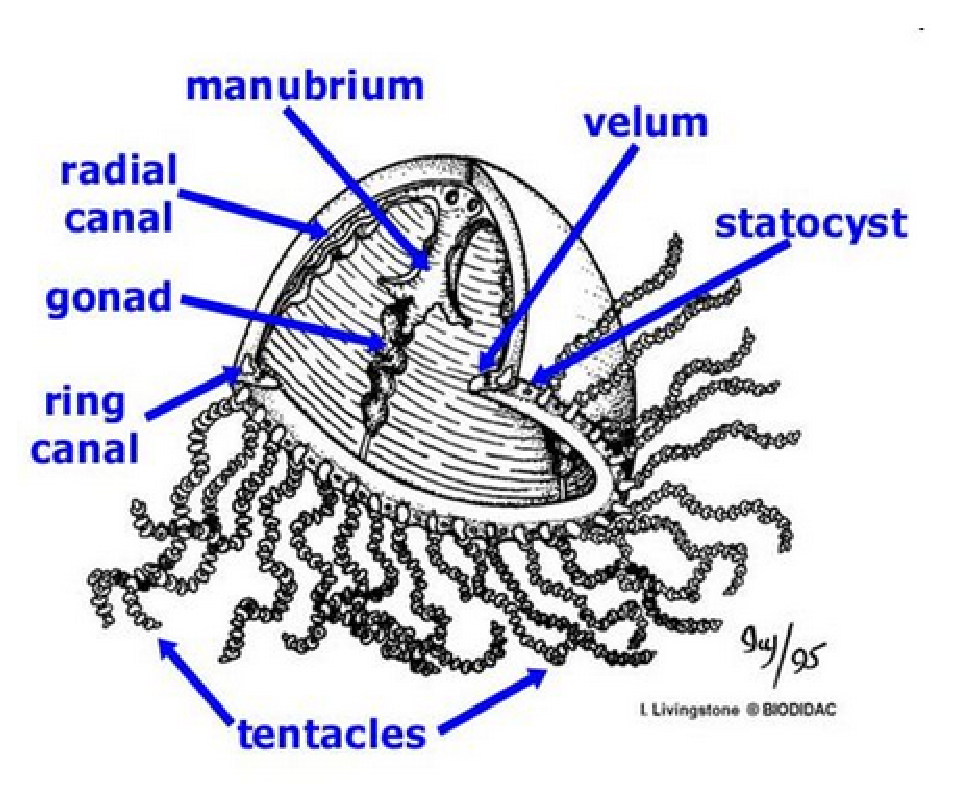
\includegraphics[height=4cm,
    angle=0]{./images/hydrozoa.eps}}
\caption{The common features of Hydra and Obelia are the presence of tissue
level of organization: single opening (act as mouth and gut), tentacles around
the mouth. NOTE: They do not have head and segmentation. }
\label{fig:hydrozoa}
\end{figure}


% \section{Metazoan's brain}

\url{https://www.google.com/search?q=single-celled+eukaryotes+calcium+action+potential&ie=utf-8&oe=utf-8}

\url{http://rstb.royalsocietypublishing.org/content/371/1685/20150043}

\url{https://en.wikipedia.org/wiki/Evolution_of_nervous_systems}



\subsection{-- Hydra's nerve net}
\label{sec:hydra}

Unlike the other cnidarians, Hydra has a remarkable power of regeneration. Under
optimum environmental conditions, these creatures used to reproduce asexually by
budding. If the water is immobile, they differentiate into male and female and
reproduce sexually by producing gametes.   

{\bf Nerve net} of Hydra is a collection of non-polar neurons that send
electrical impulses in any direction (so that the body respond to any stimulus),
e.g. control organism's movement. There can be a concentration of these nerves
around the mouth for enhanced detection of food. There is no hierarchy of
control, nor any specialization of neuronal function.



\subsection{-- Obelia's nerve net}
\label{sec:obelia-nerve-net}

Colonies of multi-celled organisms that do not have a nervous system, e.g.
Obelia, may also produce action potential. 

\begin{table}[hbt]
\begin{center}
    \begin{tabular}{p{5cm}l}
        \hline
        {\bf Polyp} & {\bf Medusa} \\
        \hline \hline
      sedentary or sessile life & adapted for a floating life \\
      non-free swimming (i.e. float moved by water and wind) & free swimming \\
      has tubular body & bell or umbrella-shaped \\
      simple body structure & complex body structure \\
      velum absent & velum present \\
      mouth is circular & mouth rectangular \\
      mesoglea: poorly developed & mesoglea: highly developed   
    \end{tabular}
\end{center}
\caption{Differences between Polyp and Medusa}
\label{tab:polyp-medusa}
\end{table}

Obelia are mainly marine and some freshwater animal species.
Obelia are usually found no deeper than 200 metres (660 ft) from the water's
surface.  They carry a nerve net with no brain or ganglia, and 2 nerve rings
at the base of velum (which creates jet propulsion).  The nerve ring, in
addition to the nerve net coordinate swimming movements.

These neurons are composed
of
\begin{enumerate}
  \item {\bf statocysts}: function in equilibrium, and respond to gravity
  
  \item {\bf ocelli}: light sensitivity
\end{enumerate}

Electrical signals can spread through the common epithelial lining of the
digestive cavity.



\section{---- Platyhelminthes (invertebrate)}
\label{sec:Platyhelminthes}



Platyhelminthes, similar to {\bf Cnidarians} (Sect.\ref{sec:cnidarians}), is an
invertebrate, Table.\ref{tab:cnidarian-platyhelminthes}.

\section{-- Echidoderm: starfish}
\label{sec:starfish-brain}

Echododerm like starfish has a locally organized nervous system, with no central
ganglion (Sect.\ref{sec:ganglion}).

The neurons of these radially symmetric organisms connect into a nerve ring,
with branches extending into each of the five arms to innervate them. This
enables organization of some movements, e.g. swimming by pulsation. 


\section{-- Worm-like hemichordate}
\label{sec:Hemichordate}

(Worm-like) Hemichordata is a phylum of marine deuterostome animals, generally
considered the sister group of the echinoderms. They appear in the Lower or
Middle Cambrian and include two main classes: Enteropneusta (acorn worms), and
Pterobranchia. 

These worms lack vertebrate-like brain. Worm-like hemichordates have a nerve net
in epidermis - which thickens to form several solid nerve cords, and a {\bf
neurocord} - a collection of giant nerve cells connected from the nerve enet.
The neurocord probably plays a role in rapid motor responses (Butler and Hodos
1996).

The last common ancestor {\it Saccoglossus kowalevskii.} (S. kowaleskii,
bottom-feeding acorn worm) - a member of Hemichordate - had with vertebrates
probably lived more than 500 million years ago.



\section{Rotifer (wheel animals)}
\label{sec:rotifer}

Rotifer are microscopic and near-microscopic pseudocoelomate animals
(mostly in 0.1-0.5 mm long; with possible range 50 $\mum$ to 2 mm).

Rotifer was first described in 1696 by  Rev. John Harris; and other forms later
described by  Antonie van Leeuwenhoek in 1703.
\begin{itemize}

  \item one or two pairs of short antennae and up to five eyes. T
  
NOTE: eyes are simple in structure, sometimes with just a single photoreceptor
cell.
  
  \item  {\bf mastax}: is the pharynx of a rotifer.
  It usually contains four horny pieces.  The two central ones form the incus,
  against which the mallei, or lateral ones, work so as to crush the food.
  
NOTE: in human: pharynx is the muscular wall - part of the throat in human that
behind the mouth and nasal cavity that function in the process of swallowing
food). 
  
  \item {\bf brain}: small (about 200 cells), and locates just above the mastax.
  The nervous system comprises about 20-25\% of the roughly 1,000 cells in a
  rotifer (Martini, 1912).
  
NOTE: \url{https://www.youtube.com/watch?v=XB_QeKO6K_U}

\end{itemize}

Electron  microscopic  investigation  of  the  rotifer nervous system revealed
the presence of dense-cored synaptic  vesicles,   which  are  supposed  to
contain catecholamines (CA). The number of the brain catecholaminergic neurons
varies from 6 to 11, constituting about 3-7\% of the total number of the brain
cells.
\begin{itemize} 
  \item  glyoxylic  acid  induced fluorescence (GAIF) method: is used to
  identify CA neurons
  
green fluorescence of CA-containing elements was observed in a fluorescent
microscope LUMAM-R3.

  \item The CA-ergic neurons, in all species studied, showed the same connection
  pattern, i.e. 
  
  Three patterns of catecholaminergic neurons
(Sect.\ref{sec:catecholaminergic-neurons}) are detected, namely: x-shaped,
arch-shaped and ring-shaped. 
  
  \item In {\it Notommata} (a species of Rotifer): 6 CA-ergic brain neurons are
  arranged in a semicircular pattern.

  \item In {\it Dicranophorus forcipatus}: 
  11 CA-ergic brain neurons form  a  ring-shaped  brain ganglion in  the
  posterior part of the head region.
  
   
\end{itemize}

A  high  degree  of concentration of CA-ergic elements can be regarded as an
indicator of the high level of development of the simple nervous system of
rotifers.



\section{Acoelomate worm (flatworm) - most primitive brain}
\label{sec:acoelomate-worm-brain}
\label{sec:flatworms}

Acoelomate worms (particularly a group called Acoela) are the most primitive
bilateral animals (other than some elongated comb jellies) and possess the most
primitive brains. 

As {\it coelom} (in Greek: having no body cavity), these worms have no
specialized circulatory and respiratory organs, which restricts them to having
flattened shapes (i.e. {\bf flatworm}) that allow oxygen and nutrients to pass
through their bodies by diffusion.

There are many different species of flatworms (e.g. Procotyla fluviatilis).
Flatworms do have brains, which are not only able to learn, but {\it regenerate
and remember} previous actions.

Flatworms have a collection of enlarged {\it anterior ganglia} - analogous to
simple brain. Longitudinal nerve cords allow some control of body movements.
\begin{enumerate}
  \item  this brain has little connection with or control over the diffuse nerve
  net throughout the rest of the body
  
  \item Acoels such as Convoluta stylifera and Otocoelis gulmariensis (and even
  turbellarians such as Xenoturbella) lack longitudinal nerves and their nervous
  system consists of a diffuse subepithelial plexus which is more developed at
  the anterior end (similar to the situation in coelenterate larvae)    
\end{enumerate}

\begin{figure}[hbt]
  \centerline{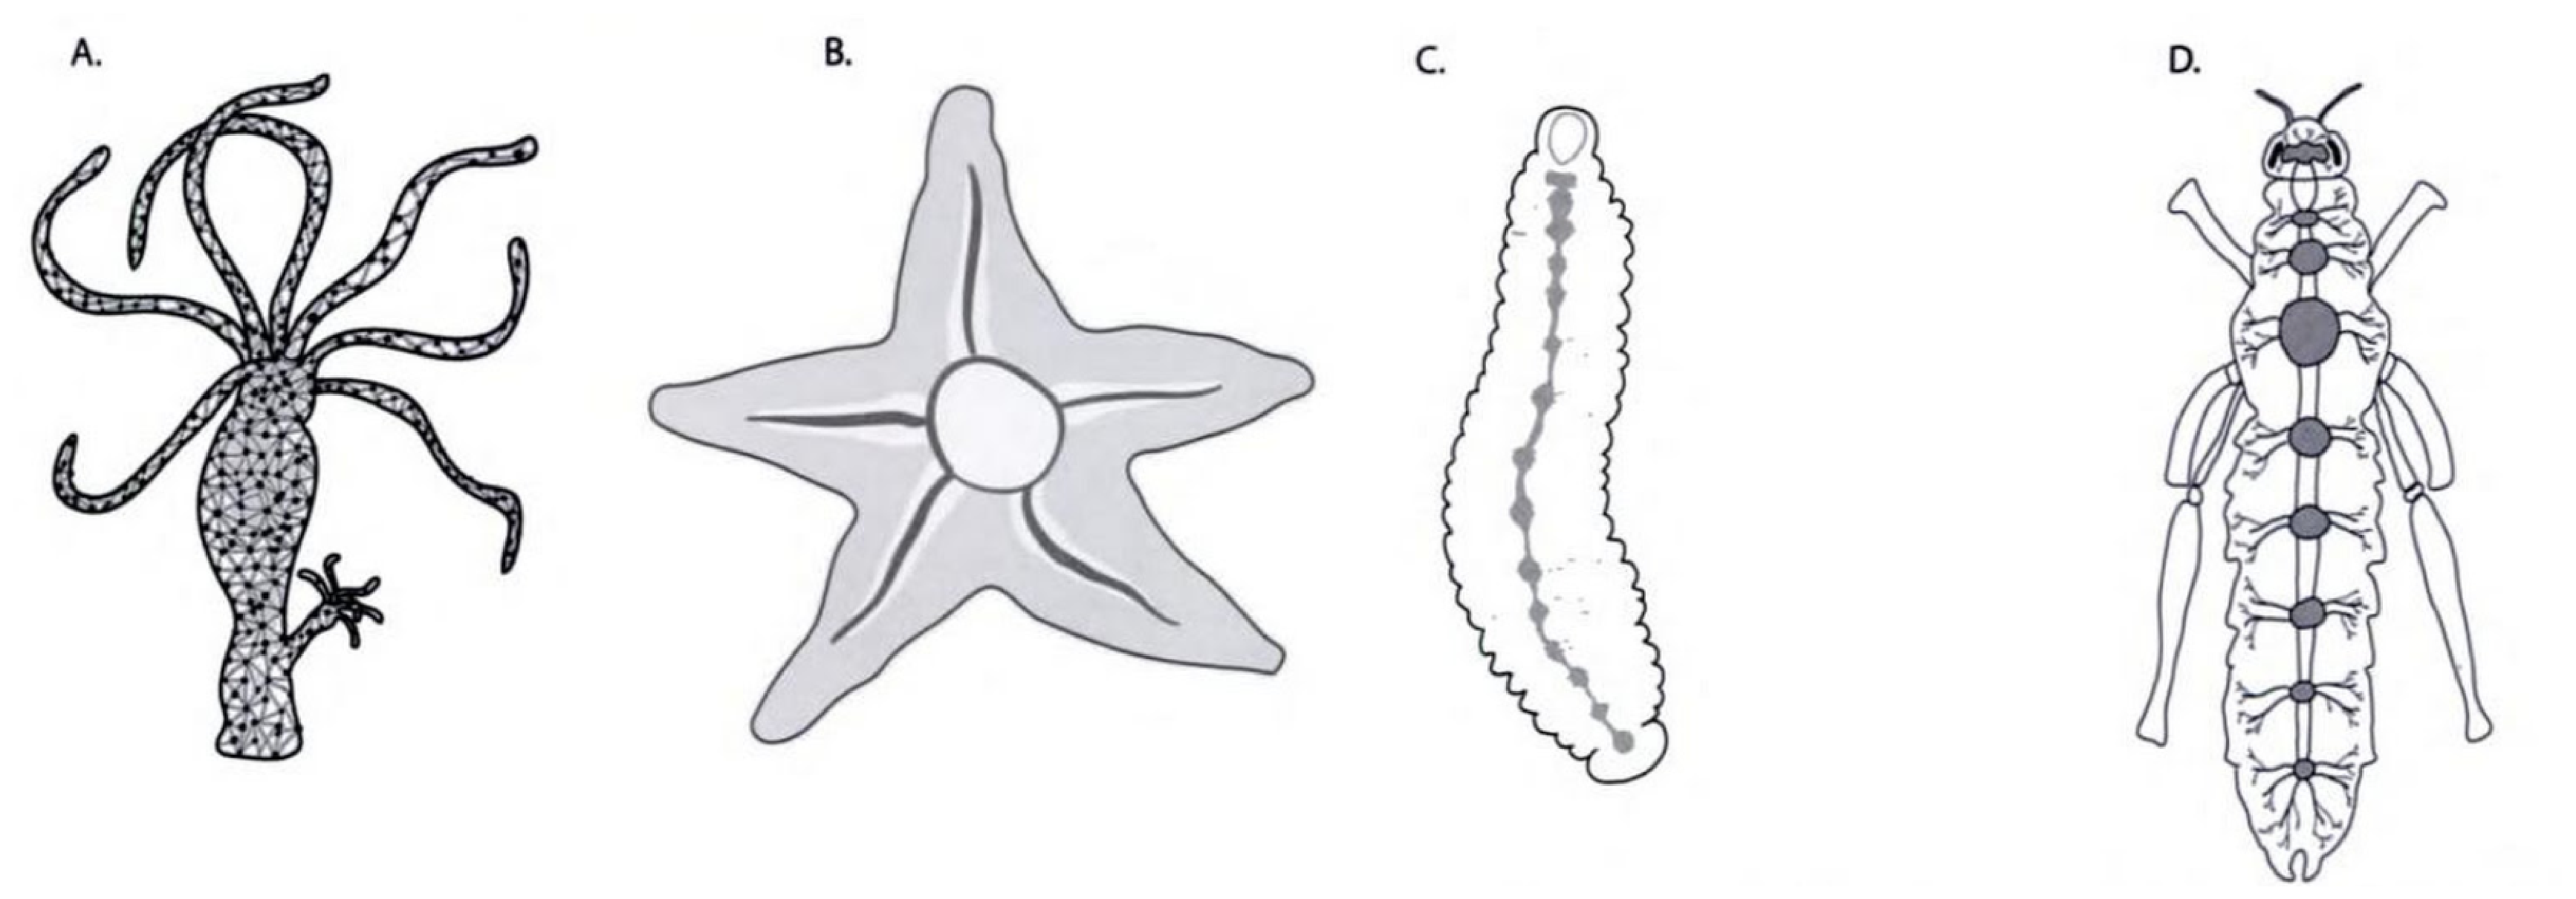
\includegraphics[height=5cm,
    angle=0]{./images/nervous-system.eps}}
\caption{Organization of early nervous systems: (A) nerve net of hydra; (B)
nerve righ of starfish; (C) leech ganglia; (D) cephalized nervous system of
grasshopper (Matthews, 2001)}
\label{fig:nervous-system}
\end{figure}

\section{Insect's brain: grasshopper}
\label{sec:insect-brain}
\label{sec:grasshopper-brain}

Although insects have brain, Fig.\ref{fig:nervous-system}(D) - their nervous
systems are much less centralized that those of vertebrates. The brain is a
collection of 6 fused ganglia (three pairs) - and each control specifically
circumscribed activities.
\begin{enumerate}
  \item {\bf protocerebrum} (first pair) : innervates the compound eyes and
  ocelli
  
  \item {\bf duetocerebrum} (second pair): integrate signals from antennae
  
  \item {\bf tritocerebrum} (third pair): innervate the labrum (i.e. roof of the
  mouth) and integrate the input from the two other pairs.
\end{enumerate}
The brain also links to the rest of the {\bf ventral nerve cord}, and the
ganglia along the cord that control organs and behaviors (e.g. feeding, mating,
locomotion, and sensory reception).

In insects, its CNS is organized as a series of ganglia - strung together along
a {\it commisure} (a junction at which corresponding structures join).
These ganglia run along the {\it ventral nerve cord}.

There are 3 kinds of neurons in the insect nervous system: 
\begin{enumerate}
  \item {\bf sensory afferents}
  
  \item {\bf motoneurons}
  
  \item {\bf interneurons}
\end{enumerate}
neurons in the CNS links the sensory and motoneurons.



\chapter{Brain's major systems}

\section{Limbic system (emotional + memory brain)}

\begin{figure}[hbt]
  \centerline{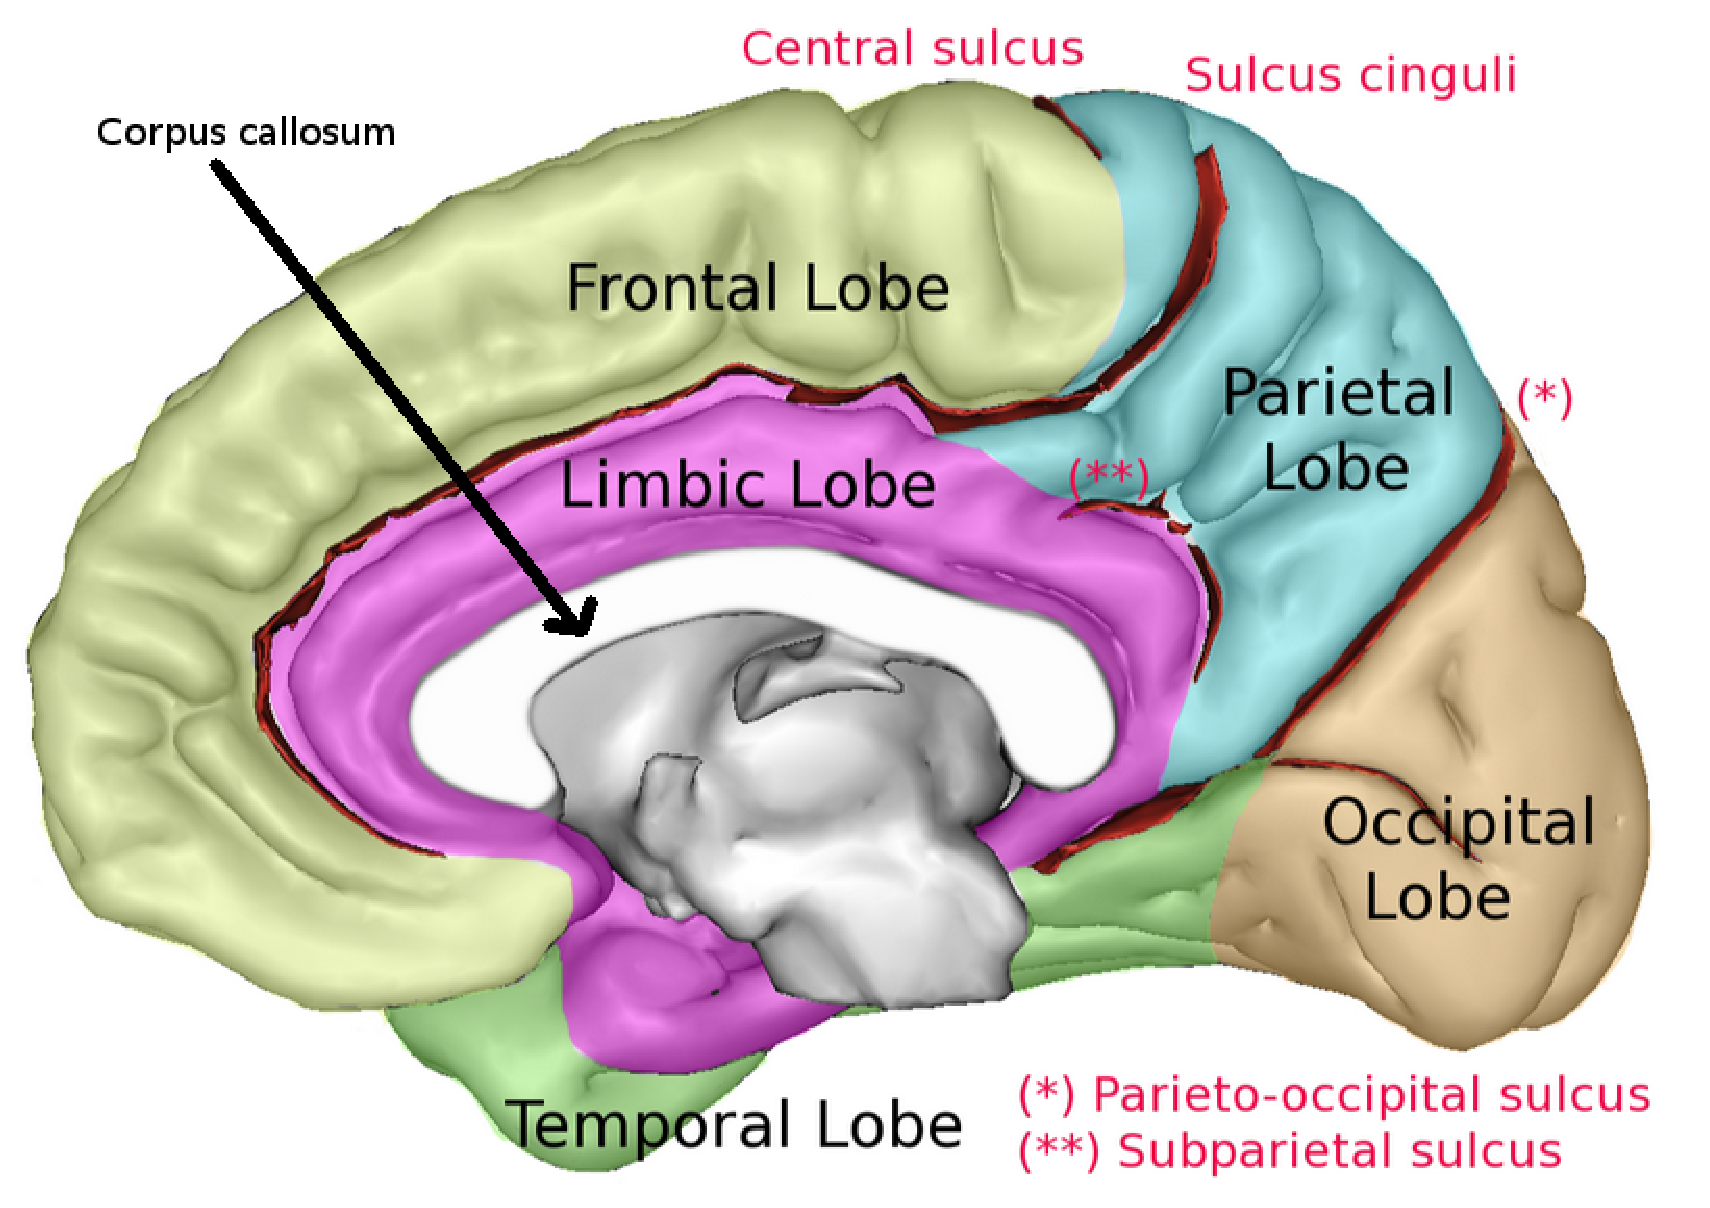
\includegraphics[height=5cm,
    angle=0]{./images/brain_lobes.eps}}
  \caption{Limbic lobe}
\label{fig:limbic_lobe}
\end{figure}

\subsection{limbic lobe (limbic gyrus)}
\label{sec:limbic-lobe}


\begin{mdframed}

The term {\bf limbic lobe} was coined by a French physician - Pierre Paul Broca
(1824-1880) in 1878 to refer to the curved rim of the cortex which includes
cingulate and the parahippocampal gyri, and associating it with the sense of
smell. NOTE: {\it limbic} is derived from Latin 'limbus' which means generally a
border, or hem or an adge.

Then, C. Judson Herrick (1868-1960) pointed out the distinction between the
lateral and medial part of the brain, i.e. the grey matter and white matter.

In 1937, James W. Papez (1883-1958) pulished a paper described the
neural circuitry that he believed might mediate the emotions \citep{papez1937}.
%The idea is that the entire limbic lobe dedicates to {\it olfaction} 
This is known as Papez circuit (Sect.\ref{sec:Papez_circuit}).

In 1948, Yakovlev proposed Yakovlev's circuit in the control of emotion
involving the orbitofrontal, insular and anterior temporal lobe cortex, the
amygdala and the dorsomedial nucleus of thalamus
(Sect.\ref{sec:Yakovlev-circuit}).

In 1949,  Paul D. MacLean published a paper that gave a new life to Papez's
theory \citep{MacLean1949}, and coined the term {\bf limbic system} to describe
Broca's limbic lobe and related subcortical nuclei in another publication in
1952 as an entire neural circuitry in the brain in charge of behavior and
emotional responses. In the modified version, a new component was added - {\bf
amygdala} and is recognized to play the important role in emotion
(Sect.\ref{sec:amygdala}).
\end{mdframed}

In 1878, Broca spoke of 'great limbic lobe' and proposed that the larger outer
gyrus be named {\bf limbic gyrus} (limbic lobe) and the smaller inner one {\bf the
intralimbic gyrus}.

Broca's limbic lobe includes 
\begin{itemize}
  \item  isthmus of the cingulate gyrus, 
  
  \item the parahippocampal gyrus and
  
  \item the subcallosal area
\end{itemize}
Both cingulate gyrus and parahippocampal gyrus are continuous via
a bundle of white matter called 'cingulum' (Sect.\ref{sec:cingulum}).

is not a concrete structure, yet it refers to an
arc-shaped (or C-shape) region situated at the inferomedial aspect of the cerebral hemispheres,
containing both gray and white matter from parts of the frontal,
parietal and temporal lobes (Sect.\ref{sec:lobes}) and form a rim around
the corpus callosum, Fig.\ref{fig:limbic_lobe}.


 such as \textcolor{red}{\bf
hippocampus} (Sect.\ref{sec:hippocampus}), and several areas in the neocortex:
piriform cortex, orbitofrontal cortex, entorhinal cortex.
A myriad of fiber tracts connect the limbic lobe with numerous deep nuclei and
the olfactory apparatus to form the limbic system
(Sect.\ref{sec:limbic-system}).
   
\subsection{limbic system (emotion brain)}
\label{sec:limbic-system}

Phylogenetically, the limbic system is one of the more primitive parts of the
brain added 150 millions year ago - Sect.\ref{sec:paleopallium}. 

The Limbic system is subdivision of the cortex, it is a network of the neuron
clusters connected by neurotransmitter pathways. It plays a role in behavior,
physiologic changes and emotions. 

The {\bf limbic system} - the ``emotion brain'', takes charges of all aspect of
emotional functions and memories, including motivation, hunger, sex, aggression,
fear, depression, stress, hallucination...
``Extreme acts of violence, suicidal behavior, agitation, and mood swings can be
due to disorders of the limbic system.''
% It has a central role in memory, learning, emotion, neuroendocrine function, and
% autonomic activities. 

\begin{figure}[hbtp]
  \centerline{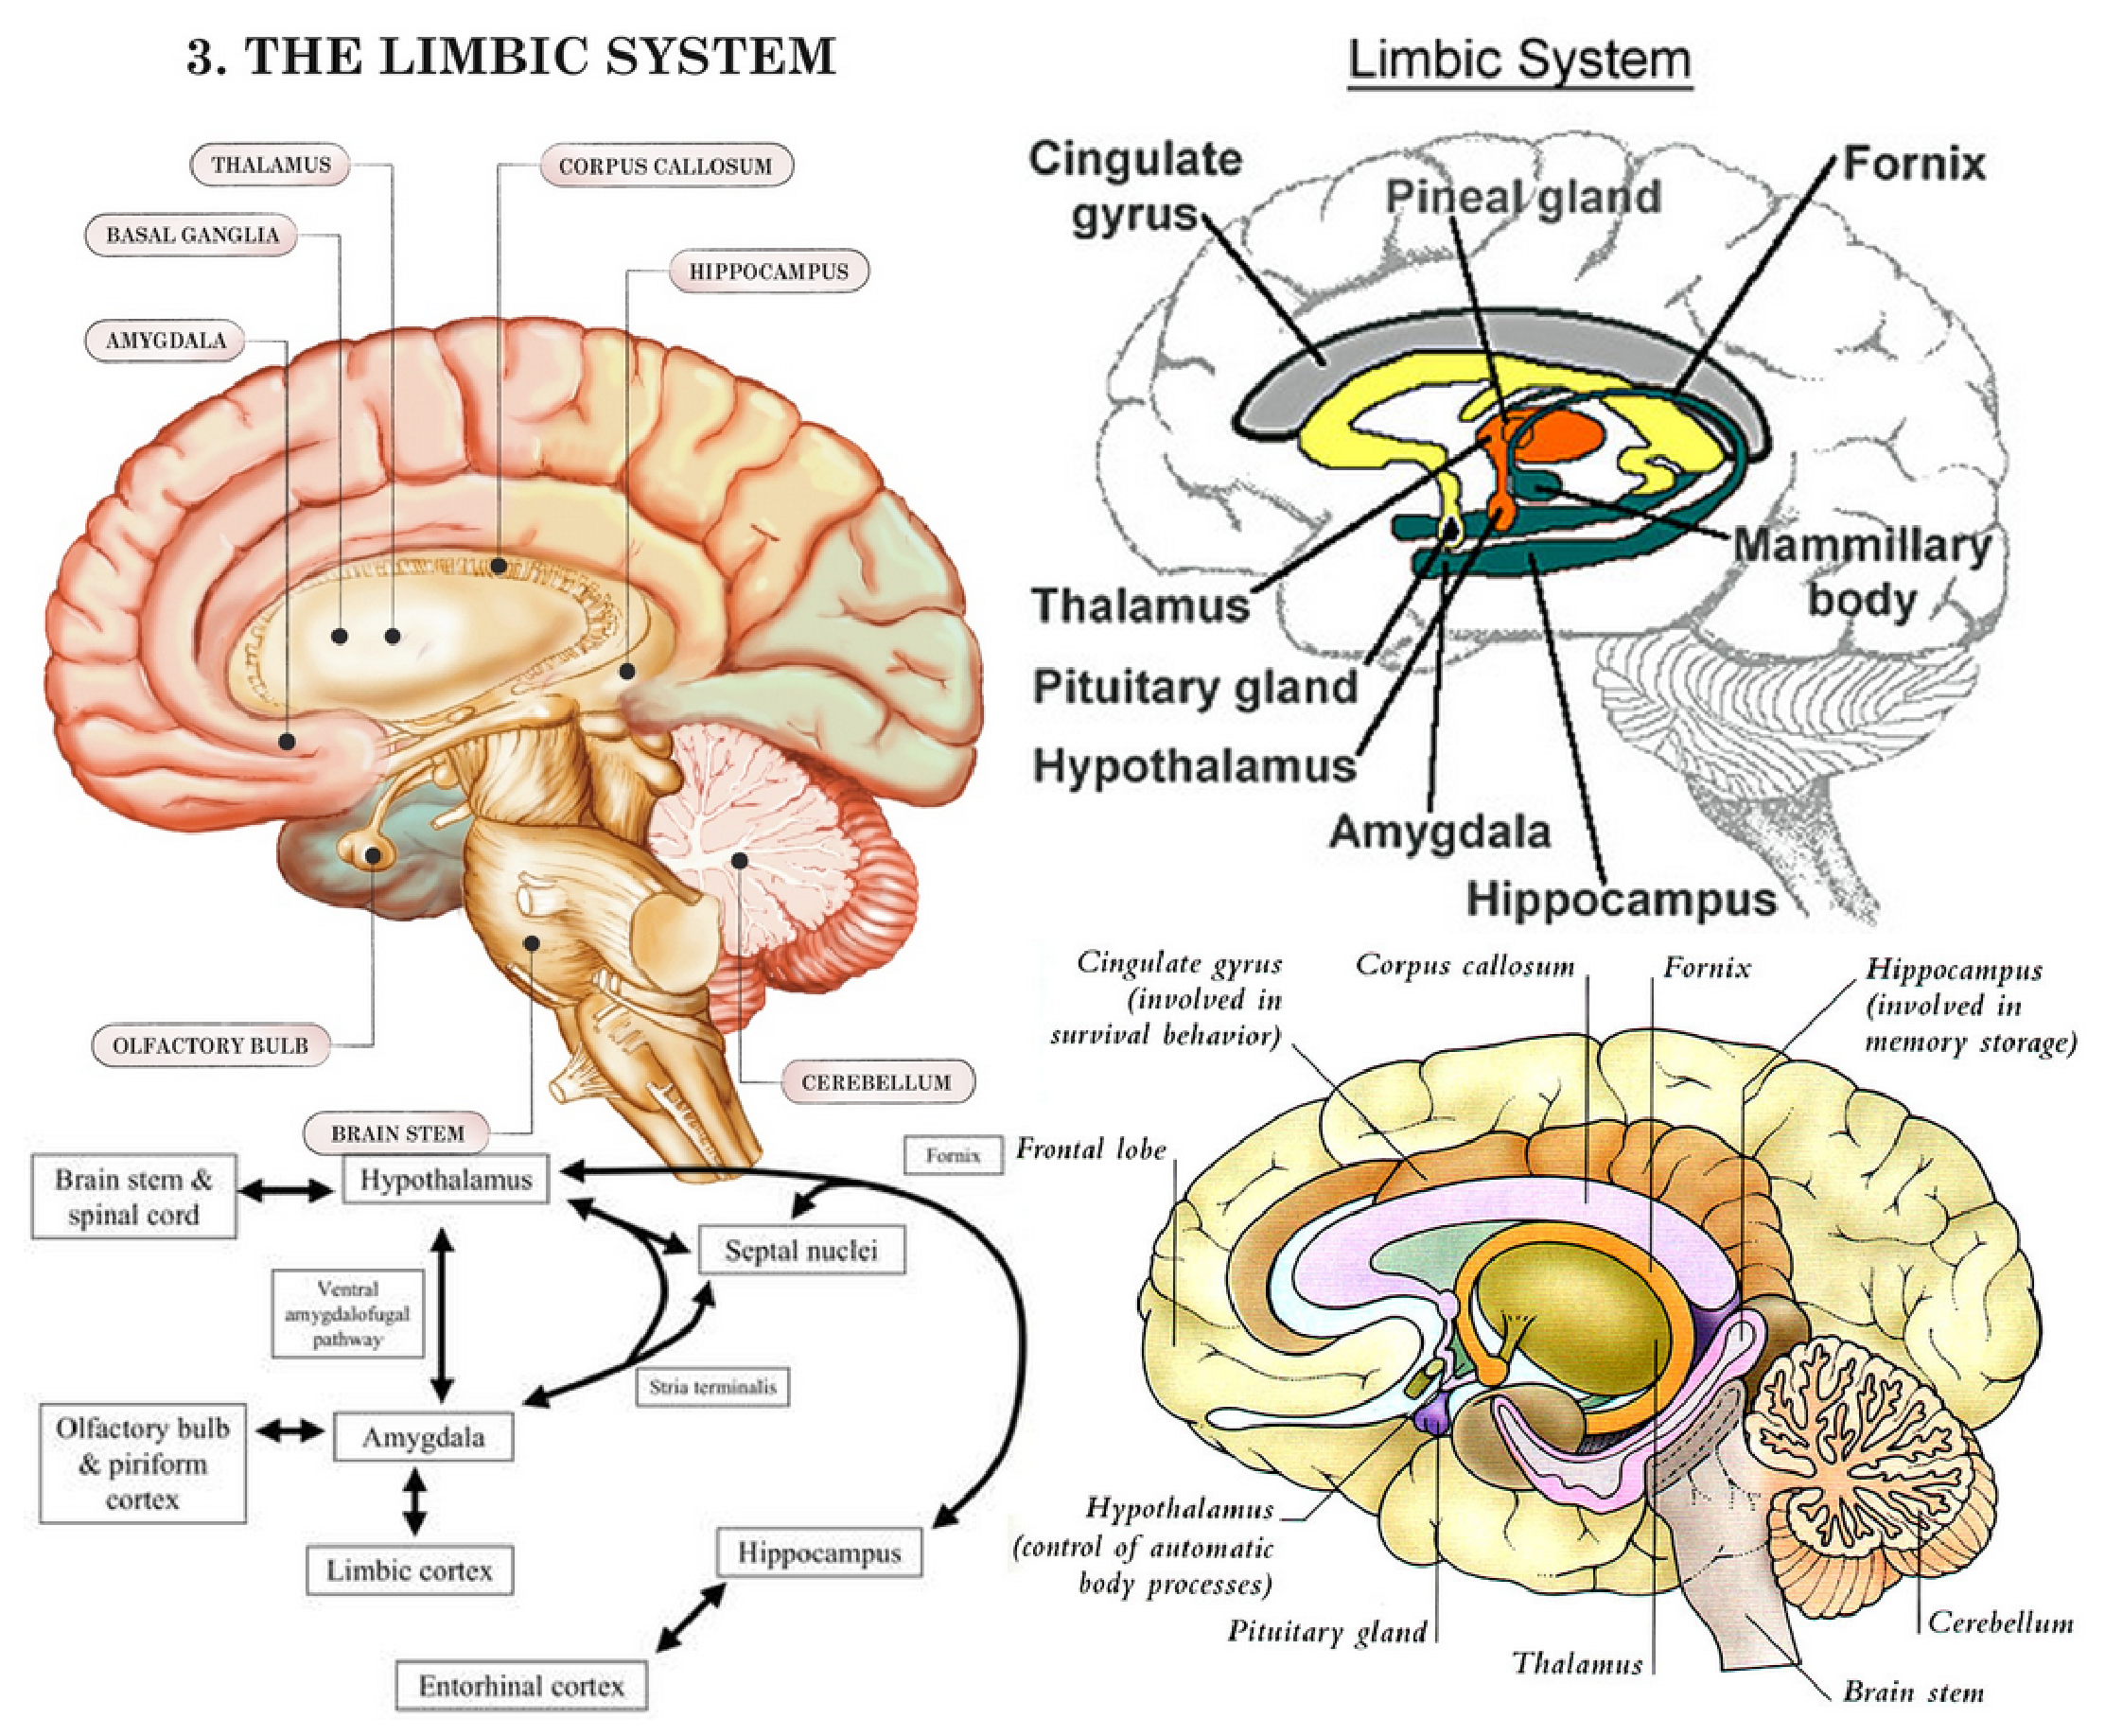
\includegraphics[height=11cm,
    angle=0]{./images/limbic_system_3.eps}}
  \caption{Components in a limbic system and its signaling pathways:
  olfactory bulb, amydgala, basal ganglia, thalamus, corpus callosum,
  hippocampus, 	cingulate gyrus, pineal gland, Fornix, mammillary body, 
  Pituitary gland
  \url{http://www.dartmouth.edu/~rswenson/NeuroSci/chapter_9.html}}
\label{fig:limbic}
\end{figure}

The limbic system is composed of several functionally and anatomically
interconnected nuclei and cortical structures, Fig.\ref{fig:limbic} extended
from the limbic lobe (Sect.\ref{sec:limbic-lobe}).
Some of these are subcortical structures  - Sect.\ref{sec:allocortex}, while
many are parts of the cerebral cortex (Sect.\ref{sec:neocortex}). However,
\textcolor{red}{the anatomical structure of the limbic system is a controversal
subject, i.e. no one know for sures which structures are parts of the limbic
system}.
% Areas that are typically included in the limbic system fall into two
% categories.
\footnote{\url{http://www.dartmouth.edu/~rswenson/NeuroSci/chapter_9.html}}

The brain regions that constitute the limbic system are:
\begin{enumerate}
  \item limbic cortex: Cingulate gyrus, Parahippocampal gyrus
  \item hippocampal formation (Sect.\ref{sec:hippocampal_formation}): dentate
  gyrus, hippocampus, subiculum 
  \item amygdala
  \item septal area
  \item hypothalamus
\end{enumerate}

Here, we discuss the 4 most important structures that everyone agree (use the
mnemonic: a hippo wearing a HAT, i.e. HAT-hippo).
\begin{itemize}
  \item Hypothalamus: Sect.\ref{sec:hypothalamus}
  \item Amygdala: Sect.\ref{sec:amygdala}
  \item Thalamus: Sect.\ref{sec:thalamus}
  \item Hippocampus: Sect.\ref{sec:hippocampus}
\end{itemize}
\url{https://www.youtube.com/watch?v=GDlDirzOSI8}

% \begin{itemize}
% 
%   \item limbic gyrus (the outer arc of limbic system and belongs to the cortical
%   areas):  subcallosal area, the cingulate gyrus
%   (Sect.\ref{sec:cingulate_gyrus}), the isthmus of the cingulate gyrus, and the
%   parahippocampal gyrus, including the uncus and subiculum.
%   %Thalamus, Hypothalamus, Amygdala
% %(rage center), Hippocampus (an important part to the memory system).
% 
%   \item Broca's intralimbic gyrus (the middle arc that belongs to subcortical
%   areas): septal nuclei, \textcolor{red}{\bf amygdala}, nucleus accumbens
%   (Sect.\ref{sec:nucleus_accumbens})
% 
% 
%   \item diencephalic structures (Sect.\ref{sec:diencephalon}):
%   \textcolor{red}{\bf thalamus}
% 
% % (i.e. diencephalon = interbrain): 4 distinct
% % components (dorsal thalamus, or simply thalamus - Sect.\ref{sec:thalamus},
% % subthalamus, hypothalamus - Sect.\ref{sec:hypothalamus}, epithalamus)
% % \url{http://en.wikipedia.org/wiki/Diencephalon}
% 
% \end{itemize}


% 
% \begin{figure}[hbt]
%   \centerline{\includegraphics[height=5cm,
%     angle=0]{./images/limbic_system.eps}}
%   \caption{(A) Outside side view of the brain, (B) the limbic system }
% \label{fig:limbic}
% \end{figure}
\subsection{Input/Output}

So, we have the cerebrum as 'thinking brain' (Sect.\ref{sec:cerebrum}), and
limbic system as 'emotional brain' or 'feeling and reacting brain'. The signal
from the 'thinking brain' go through this emotion brain before going to the
other parts of the body.
In this construct, the limbic system is usually under control of the "thinking
brain" but obviously can react on its own. In the limbic system:
\begin{itemize}
  \item the input side and processing side: limbic cortex
  (Sect.\ref{sec:limbic_cortex}), amygdala (Sect.\ref{sec:amygdala}) and
  hippocampus (Sect.\ref{sec:hippocampus})
  
  \item the output side: septal nuclei (Sect.\ref{sec:septal_nuclei}) and
  hypothalamus (Sect.\ref{sec:hypothalamus})
\end{itemize}
Most of these regions are interconnected  by pathways given in
Fig.\ref{fig:limbic}.

\subsection{Thalamus (dorsal thalamus): isothalamus}
\label{sec:thalamus}
\label{sec:dorsal-thalamus}

The term thalamus can refer to the collective of different structure
(Sect.\ref{sec:diencephalon}). However, in many cases, {\bf thalamus} means {\bf
dorsal thalamus}, from that different structures are named based on relative
position to the thalamus, e.g. subthalamus, hypothalamus.

The thalamus is considered as the gateway to the cortex, as it receives all
sensory inputs from posterior column (i.e. dorsal horn) of spinal cord -
Sect.\ref{sec:posterior-grey-column}.

The neurons in the thalamus include interneurons
(Sect.\ref{sec:thalamic-interneurons}) and thalamocortical neuron -
Sect.\ref{sec:thalamocortical-neuron}.

{\bf Dorsal thalamus} is a subcortical region, and there are two of them (left
and right side of the hemisphere), Fig.\ref{fig:thalamus}. It is a part of the
diencephalon (Sect.\ref{sec:diencephalon}) - a nuclear complex structure of 4
parts: hypothalamus - Sect.\ref{sec:hypothalamus}, epithalamus -
Sect.\ref{sec:epithalamus}, prethalamus (subthalamus, formerly 'ventral
thalamus' - Sect.\ref{sec:subthalamus}) and dorsal thalamus (often call
thalamus).


\subsection{-- Thalamus' function}
\label{sec:thalamus-function}

The thalamus receives signals from projection neurons in the posterior columns
of spinal cord - Sect.\ref{sec:posterior-grey-column}.

Because of this, the thalamus is believed to relays sensory impulses from
receptors in various parts of the body to the relevant region in the
subcortical areas (e.g. striatum of the basal ganglia) and the cerebral
cortex (Sect.\ref{sec:cerebral-cortex}) for processing
\begin{itemize}
  \item relay sensory input to sensory cortex, e.g. visual cortex and auditory
  cortex - Sect.\ref{sec:visual-cortex}.

  In other words, all sensory information (the things that we see, hear, touch)
  is conveyed through the thalamus structure, and then the thalamus will
  redirect the signal to the right regions in the brain. Damaged to the thalamus
  can lead to permanent coma. 
  
  \item relay motor signals to motor cortex - Sect.\ref{sec:motor-cortex}


\end{itemize}
\textcolor{blue}{The only sensory information that is not relayed by the
thalamus into the cerebral cortex} is information related to smell (olfaction) -
Sect.\ref{sec:olfactory-bulb}, although in higher level processing, correlating
smells with memories, etc, it will go through the thalamus.
% Emotion sensings relate to what you see, hear and touch. There is another
% emotional sensing, \textcolor{red}{the sense of smell - which is the only one
% that bypasses the thalamus}.

Nowadays, there are evidences that the thalamus not only relay information, but
also process it, as the neurons in the primary sensory relay also receive the
feedback from the cerebral cortex ({\it back injections}).

{\small Sect.\ref{chap:Retina} for retina
\begin{verbatim}
retina input ---[optic nerve] ---- LGN ---
              ----[relay]--> primary visual cortex (V1) 
                             in occipital lobe
              
auditory input ---]               medial geniculate nucleus 
\end{verbatim}
}

The thalamus is involved in many functions that cannot be considered as sensory
or motor. The projection from the thalamus to the cortex uses the internal
capsule (Sect.\ref{sec:internal_capsule}), both the anterior and posterior limbs. This
portion of the internal capsule is called {\it thalamic radiation}.

A significant reduced in volume of thalamus has been found  individuals with
schizophrenia and Schizoaffective (review: \citep{smith2011}).

\subsection{-- Thalamus's nuclei}

\textcolor{red}{\bf NUCLEI}: The neurons in the thalamus are grouped into
different nucleus structures (Sect.\ref{sec:nuclei_structure}) with distinct
functions, giving the functional complexity of the thalamus. 

\begin{figure}[htb]
\centerline{\includegraphics[height=11cm]{./images/thalamus.eps}}
\caption{Major divisions in the thalamus}\label{fig:thalamus}
\end{figure} 

% \textcolor{red}{There are the six thalamic nuclei that receives the projections
% from the STT and TTT of trigeminal brainstem nuclear complex (TBNC)
% (Sect.\ref{sec:TBNC})}.
% \footnote{\url{http://www.neuroanatomy.wisc.edu/coursebook/thalamus.pdf}}
% \begin{enumerate}
%   \item {\bf ventral posterior nuclei} (VP: VPL, VPM, VPI): the main
%   somatosensory nuclei of the thalamus $\leftarrow$ receive input 
%   from the main sensory nuclelus (MSN) of TBNC (Sect.\ref{sec:TBNC}), and
%   (mechanoreceptive information from) dorsal column nuclei (DCN)
%   
%   Most neurons in VP responds to low-threshold mechanoreceptive input.
%   
%   VPM and VPL are called internal and external portions of the ventral caudal
%   (Vc) nucleus; while VPI is called the parvicellular part of the ventral caudal
%   nuclei (Vcpc).
%   \begin{itemize}
%     \item VPM (ventroposterior medial nucleus): receive sensory inputs from the
%     body: 
% %   receive inputs from the {\it dorsal column-medial lemniscus
% % %   pathway} (DC-ML, Sect.\ref{sec:DCML}), LSTT to the VPL
% 
% % receive inputs from the {\it trigeminothalamic tract} (TTT)
% %   and {\it spinothalamic tract} (STT) to {\it ventro-posteromedial} (VPM)
% %   nucleus.
%         
%     \item VPL (ventroposterolateral nucleus): receive sensory inputs from the
%     head and face via trigeminal nerve (Sect.\ref{sec:trigeminal-nerve})
%     
% \begin{verbatim}
%     Neurons in laminal IV-V of STT and TTT of TBNC [sensory input from
%     head/face] ----> to VPL in thalamus (of neurons that 
%                      are immunoreactive to calbidin)
% \end{verbatim}    
% 
%     VPL is further divided into 
%     \begin{itemize}
%       \item major portion: receives innoculous tactile information, and project
%       to areas 3b and area 1 of the primary somatosensory cortex
%       
%       \item anteriorly located shell region: receives proprioceptive information
%       (muscle and joint afferent) and project to area 3a and area 2
%       (Sect.\ref{sec:area_in_brain})
%       
%        \item VPI (ventrally adjacent region called ventroposterior inferior
%     nucleus): project to second somatosensory cortex (Sect.\ref{sec:somatosensory-cortex})
%     \end{itemize} 
%   \end{itemize}
%   
%   \item {\bf posterior portion of the ventral medial nucleus} (VMpo)
%   
%   \item {\bf ventral lateral nucleus} (VL)
%   
%   \item {\bf central lateral nucleus} (CL)
%   
%   \item {\bf parafascicular nucleus} (Pf)
%   
%   \item {\bf ventral caudal portion of the medial dorsal nucleus} (MDvc)
% \end{enumerate}

The six thalamic nuclei are organized as follows, starting from the posterior of
the thalamus, i.e. Level 11
\begin{enumerate}
  \item Level 11: has 2 nucleus

   \begin{itemize}
       \item {\bf MGB (MGN)} (medial geniculate body, medial geniculate
    nuclelus): is an auditory relay nuclei
    
    INPUT: visual signals from superficial layers of superior colliculus
    
    OUTPUT: project to the primary visual cortex (area 17, V1)

MGB is subdivided  into sub-nuclei: ventral (VMGB), dorsal (DMGB) and medial
(MMGB); with VMGB is specific to auditory input, the other twos (DMGB, MMGB)
also receive non-auditory input.

        \item {\bf LGB (LGN)} (lateral geniculate body, lateral geniculate
  nuclei): is a visual relay nuclei
  
	INPUT: auditory signals from inferior colliculus 
	
	OUTPUT: project to the primary	auditory (area 41,42) cortical areas.

   \end{itemize}

  \item Level 12: 
  {\bf ventral posterior nuclei} (VP, VPN) is the main
  somatosensory nuclei of the thalamus $\leftarrow$ receive input
  from the main sensory nuclelus (MSN) of TBNC (Sect.\ref{sec:TBNC}), and
  (mechanoreceptive information from) dorsal column nuclei (DCN)

  Most neurons in VP responds to low-threshold mechanoreceptive input.

 VP is constituted by VPL, VPM, VPI, and VMpo: the 
  VPM and VPL are called internal and external portions of the ventral caudal
  (Vc) nucleus; while VPI is called the parvicellular part of the ventral caudal
  nuclei (Vcpc); the location of  {\bf posterior portion of the ventral medial
  nucleus} (VMpo) is uncertain and is considered as a satellite of the VP
  complex.
  
   \begin{itemize}
      \item VPM (ventroposterior medial nucleus): receive sensory inputs from
     the body via the {\it dorsal column-medial lemniscus
     pathway} (DC-ML, Sect.\ref{sec:DCML}) %, LSTT to the VPL

% receive inputs from the {\it trigeminothalamic tract} (TTT)
%   and {\it spinothalamic tract} (STT) to {\it ventro-posteromedial} (VPM)
%   nucleus.

      \item VPL (ventroposterolateral nucleus): receive sensory inputs from the
    head and face via trigeminal nerve (Sect.\ref{sec:trigeminal-nerve})

{\small
\begin{verbatim}
Neurons in laminal IV-V of STT and TTT of TBNC [sensory input from
    head/face] ----> to VPL in thalamus (of neurons that
                     are immunoreactive to calbidin)
\end{verbatim}
}
    VPL is further divided into
       \begin{itemize}
          \item major portion: receives innoculous tactile information, and
       project to areas 3b and area 1 of the primary somatosensory cortex

          \item anteriorly located shell region: receives proprioceptive
      information (muscle and joint afferent) and project to area 3a and area 2
      (Sect.\ref{sec:area_in_brain})

      \end{itemize}

      \item VPI (ventrally adjacent region called ventroposterior inferior
    nucleus): project to second somatosensory cortex (Sect.\ref{sec:somatosensory-cortex})
    
      \item VMpo: the cells here signals pain and temperature 
   \end{itemize}

%   both project to the primary somatosensory cortex
%   (Sect.\ref{sec:somatosensory-cortex})
% \begin{itemize}
%   \item {\bf VPN}: 
%   
%   \item {\bf VPL}: 
%   \end{itemize}

  \item Pulvinar nuclei:  subdivided into anterior, inferior, lateral, and
  medial subdivisions, each containing multiple nuclei.
  
It is virtually nonexistent in the rat; but in humans, it makes up 40\% of
the thelamus.
  
  \item Level 15: these two nuclei are the motor relay nuclei,
receiving inputs from the cerebellum and the basal ganglia
 \begin{itemize}
   \item {\bf VA} (ventral anterior nucleus): 
  
    INPUT: from globus pallidus
   
    OUTPUT (providing feedback for the output of basal ganglia): to premotor
    cortex for initiation and planning movement
    
   
   \item {\bf VL} (ventral lateral nucleus):
   
 
   INPUT: from substantia nigra and globus pallidus (via thalamic fasciculus);
   and from cerebellum ((via the dentatothalamic tract))
   
   OUTPUT: to primary motor cortex and premotor cortex.
 \end{itemize} 
\end{enumerate}


The remaining thalamic nuclei are
\begin{enumerate}
  \item {\bf MD} (medial dorsal):  it is present through most of the
  rostrocaudal extent of the thalamus (most obvious in Level 13).

This is the only nucleus in the medial group, and it receives two kinds of
inputs: (1) pain afferents from the {\it lateral spinothalamic tracts} (LSTT)
and the TTT, projects to the frontal lobe, and
is involved in the response to pain; (2)  receives olfactory inputs from primary
olfactory cortex.

This nucleus is unique because it receives these olfactory inputs after they
have been to cortex, and then relays them to insular
(Sect.\ref{sec:insular-cortex}) and orbitofrontal cortex for associative olfactory functions.

  \item {\bf Ant} (Anterior nuclear group):  its association with the internal
medullary lamina (IML).

  \label{sec:centromedial_nucleus}
  \item {\bf CM} (centromedian nucleus): 
  {\bf Centromedian nucleus} (centrum medianum, CM, Cm-Pf) 
is a part of the intralaminar nucleus (ILN) of the thalamus. There are two
centromedian nuclei arranged bilaterally. It has about 664,000 neurons in total,
i.e. 2000 neurons per cubic millimetre and has a volume of about 310 cubic
millimetres.
  \url{http://en.wikipedia.org/wiki/Centromedian_nucleus}

We know very little about this nucleus due to its deep location, but we do
know that it has some major connections to the motor systems basal ganglia.
\end{enumerate}


To make it simpler, the term {\bf isothalamus} is used by some researchers to a
division, constituted more than 90\% of the thalamus and comprises by two types
of neurons: thalamocortical fibers (a bush or tree-like apperance structures of
thalamocortical neurons - Sect.\ref{sec:thalamocortical-neuron}) and
microneurons (Sect.\ref{sec:microneurons}) (see below for details).

There are 3 types of neurons in the thalamus:
\begin{enumerate}
  \item thalamocortical neurons (TC) - Sect.\ref{sec:thalamocortical-neuron}:
  
  \item reticular neurons (RE) - Sect.\ref{sec:reticular-neuron}:  
  
  \item thalamic interneurons - Sect.\ref{sec:thalamic-interneurons}:
\end{enumerate}




\subsection{Amygdala}
\label{sec:amygdala}

{\bf Amygdala} (pl: amygdalae) (aka central medial amygdala) is an almond-shape
masses of neurons at the lower end of the hippocampus. There are two of them,
one on each hemisphere, Fig.\ref{fig:amygdala}.
{\bf Extended amygdala} is a macrostructure that includes
\begin{itemize}
  \item (central medial) amygdala: (discuss in this section)
  
  \item substantia innominata: a stratum consisting of gray and white substance
  which is part of the basal forebrain (Sect.\ref{sec:basal-forebrain}).
  
  \item the shell of nucleus accumbens (Sect.\ref{sec:nucleus_accumbens})
  
  \item stria terminalis: the band of fiber serving as the major output pathway
  of the amygdala.
\end{itemize}


Amygdala was first identified by Burdach in the early 19th century, with the
group of cells called basolateral complex.
Subsequently, a large number of structures that surround the basolateral complex
have been identified in many species and constitute what is now known as the
{\bf amygdaloid complex} \citep{sah2003amygdala}. 

Nowadays, the amygdala has several different nuclei and internal pathways, with
the most well-known are (each has a unique function and purpose)
\begin{itemize}
  \item basolateral complex (or {\bf basolateral amygdala} - BLA) 
  \item centromedial nucleus (CM): Sect.\ref{sec:centromedial_nucleus} 
  \item cortical nucleus
\end{itemize}

\begin{figure}[hbt]
  \centerline{
  \includegraphics[height=4cm,
    angle=0]{./images/amygdala.eps}}
\caption{Amygdala}
\label{fig:amygdala}
\end{figure}

{\bf Basolateral complex} (basolateral amygdala) refers to the group of
structures: lateral, basal and accessory-basal nuclei of the amygdala.
The primary function of the basolateral complex is stimulating fear response.
\begin{itemize}
  \item lateral nuclei: receive that majority of sensory information arrived
  directly from temporal lobe structures, including hippocampus and
  primary auditory cortex. 

The input is processed by the basolateral complex, and then the output is sent
to the centromedial nucleus of the amygdala.
  
  \item 
\end{itemize}

Amygdala is also called agression center, as the stimuli of this region can 
produce anger, violence, fear, anxiety. The destruction of the 
amygdala can cause a mellowing effect (i.e. smooth, pleasant), which
was noted by two doctors Kluver and Bucy. The
destruction of both amygdala (i.e. bilateral destruction) can cause several
symptoms: 
\begin{itemize}
  \item hyperorality: you put things in your mouth a lot
  \item hypersexuality: 
  \item disinhibited behavior: you ignore social conventions (i.e. doing
  dangerous, reckeless things)
\end{itemize}
This was called Kluver-Bucy syndrome. This is similar to drinking alcohol.
 
Neurons in amydgala relate to anger. In animals, when these neurones stimulated
by electrical signals, animals become aggression. If these neurons are damaged,
the animals become very tamed. It's more than just anger. Without neurons in
amydgala, animals becomes indifferent to stimuli that previously have caused
fear or even sexual
responses\footnote{\url{http://webspace.ship.edu/cgboer/libicsystem.html}}.


\subsection{Hypothalamus}
\label{sec:hypothalamus}

Hypothalamus (Hypo- = below) is a very tiny structure (less than 1\% the total
volume of the brain, i.e. about the size of the kidney brain).


As you can see in Fig.\ref{fig:limbic}, the hypothalamus connects with the brain
stem and spinal cord to receive signal from the autonomic nervous system
(Sect.\ref{sec:autonomic_nervous_system}). Thus, {\bf hypothalamus} is the {\it
primary output node} (i.e. the center) of the limbic system.
Currently, human hypothalamic cells are largely inaccessible for direct
study.

\subsection{-- function}
\label{sec:hypothalamus-functions}

By sensing the changes in various internal organs, \textcolor{red}{hypothalamus
is the central part for controlling the endocrine system}
(Chap.\ref{chap:Endocrine-System}). The neuroendocrine system is the mechanism
by which the hypothalamus maintains homeostasis, regulating reproduction,
metabolism, eating and drinking behaviour, energy utilization, osmolarity and
blood pressure. Hypothalamus is one of the busiest part in the brain, and is
mainly concerned with

\begin{enumerate}
  
  \item intrinsic functions: 
  
  \begin{itemize}
    
    \item (1) homeostasis, e.g. regulating your hunger, thirst, response to
    pain, levels of pleasure, sexual satisfaction, anger,
  aggressive behavior...

  \begin{figure}[hbt]
  \centerline{\includegraphics[height=6cm,
    angle=0]{./images/hypothalamus.eps}}
\caption{Hypothalamus and two wing-like structures  called suprachiasmatic
nucleus (SCN). A protein inside the soma of the nerve cell in SCN is the
product of a biological clock gene}
\label{fig:hypothalamus}
%http://www.hhmi.org/biointeractive/human-suprachiasmatic-nucleus
\end{figure}
    
    \item (2) circadian clock: 
    
  {\bf suprachiasmatic nucleus} (SCN) is a tiny region (pair, wing-like
  structure) in the hypothalamus as shown in yellow color in
  Fig.\ref{fig:hypothalamus}. SCN is situated directly above the {\it optic
  chiasm} [NOTE: suprachiasmatic means "above the chiasm"]. SCN contains a few
  thousands nerve cells which receives direct retinal input. 

  {\it Light enters the eye and activate neurons in the retina that convert
  photon energy into electrical signals, which then transfers via the long axon
  of retinal neurons into the optic nerve. Along the way of signal transmission,
  the {\bf optic chiasm} is the region where the signal from left and right eyes
  meet and cross, which then continue into 2 paths}
  \begin{enumerate}
    \item toward the back of the   brain where it is processed into images that
    can be consciously perceive	
  
     \item (carrying the information to SCN) exit the optic chiasm and turns
     upward, toward the SCN 
  \end{enumerate}

  \textcolor{blue}{This nucleus is responsible for our biological clock}, i.e.
  generating signals that can keep the body 24-hours schedule (circadian rhythms
  to the day-night cycle).
  \footnote{\url{http://www.hhmi.org/biointeractive/human-suprachiasmatic-nucleus}}
  However, because the internal clock's period is not exactly 24 hours,
  environmental cues - most importantly, light - are required to reset the clock
  each morning and keep the organism in sync with the external world.
  These neurons inside fires with a circadian rhythm.
  Inside a single SCN neuron, the protein product of a biological clock gene
  turns off production of more protein, forming a negative feedback loop. 
  
  \end{itemize}
  
     
  \item It also influences/regulates the functioning of the
\begin{itemize}
  \item  (1) {\it autonomic nervous system}, e.g. things like pulse, blood
  pressure, breathing and arousal in response to emotional circumstances.

It influences autonomic functions via synaptic projections to the brain stem and
spinal cord. There are localized areas in the hypothalamus that will activate
the sympathetic nervous system and some that will increase parasympathetic activity.
  
There are also projections to the reticular formation that are involved in
certain behaviors, particularly emotional reactions.
     
  \item (2) releasing hormones for endocrine functions and behaviors:
  Chap.\ref{sec:glands-head-neck}   
\end{itemize}  

   \item Additionally, there are many complex behaviors that are patterned by the
hypothalamus, including sexual responses. The preoptic area is one of the areas
of greatest sexual dimorphism (i.e., difference in structure between the sexes)
and, along with the septal nuclei, is an area of gonadotropin releasing hormone
projections to the median eminence region of the hypothalamus. These sexual
responses involve autonomic, endocrine and behavioral responses.

\end{enumerate}

\subsection{-- structure}

It contains a number of small nuclei with a variety of functions
(Sect.\ref{sec:hypothalamus-functions}); one of that is linking the nervous
system to the endocrine system via the pituitary gland
(Sect.\ref{sec:pituitary-gland}).

The hypothalamus is divided into anterior, tuberal, and
posterior regions, each region has a few areas, and the nucleus can be inside
one area, or spread across many areas:
\begin{enumerate}
  
  \item \textcolor{red}{anterior region}: 3 areas
  \begin{itemize}
    \item preoptic area: {\bf preoptic nucleus}
    \item medial area: {\bf medial preoptic nucleus}, supraoptic nucleus, {\bf
    paraventricular nucleus}, anterior hypothalamic nucleus, {\bf
    suprachiasmatic nucleus}
    \item lateral area: {\bf lateral nucleus}
  \end{itemize}
  
  \item \textcolor{red}{tuberal region}: 2 areas
  \begin{itemize}
    \item medial area: {\bf dorsomedial hypothalamic nucleus}, ventromedial
    nucleus, {\bf arcuate nucleus}
    
    \item lateral area: {\bf lateral nucleus}, lateral tuberal nucleus
  \end{itemize}
  
  \item \textcolor{red}{posterior region}: 2 areas
  \begin{itemize}
    \item medial area: {\bf mammillary nuclei}, posterior nucleus
    
    \item lateral area: {\bf lateral nucleus}, tuberomammillary nucleus
  \end{itemize}
  \end{enumerate}
\url{https://en.wikipedia.org/wiki/Hypothalamus#Nuclei}

\textcolor{red}{NUCLEI}: Constituent cell bodies with distinct physiological
functions reside in these different nuclei
\begin{enumerate}
  
    \item {\bf paraventricular hypothalamus nucleus} (PVN, PVA, PVH): cells are
    magnocellular neurosecretory cells (Sect.\ref{sec:magn-neur-cells})

  
   Many PVN neurons project directly to the posterior pituitary where they
   release oxytocin or vasopressin into the general circulation.

\url{https://en.wikipedia.org/wiki/Paraventricular_nucleus_of_hypothalamus}

  \item  {\bf supraoptic nucleus}  (SON): In humans, it contains about 3,000
  magnocellular neurosecretory cells (Sect.\ref{sec:magn-neur-cells})
  
   \item ventromedial nucleus 
   
   \item arcuate ventromedial hypothalamus (VMH) nuclei: neurons expressing
   proopiomelanocortin (POMC) and neuropeptide Y (NPY)/agouti-related peptide
   (AGRP), can sense peripheral hormones - insulin, leptin, ghrelin, PYY - and
   secrete neuropeptides $\alpha$ melanocyte-stimulating hormone ($\alpha$MSH)
   and NPY/AGRP to engage receptors on so-called 'second order' DMH, PVH, and
   other neurons to regulate aspects of energy homeostasis through melanocortin
   4 receptor (MC4R), neuropeptide Y receptor type 1 (NPY1R), and other
   receptors
   
   \item {\bf dorsal medial} hypothalamus (DMH) nuclei 
  
   \ldots
  
\end{enumerate}
\subsection{-- connectivity}
\label{sec:hypothalamus-connectivity}

Most nerve fibres within the hypothalamus run in two ways (bidirectional).

\textcolor{red}{\bf INPUT CONNECTIVITY}: 
To perform its essential functions, hypothalamus requires several types of input
from many others parts of the limbic system.
\begin{itemize}
  \item receive inputs from hippocampus (Sect.\ref{sec:hippocampus}) via the
  fornix (Sect.\ref{sec:Fornix}), and from
  amygdala(Sect.\ref{sec:amygdala}) via 2 pathways (ventral amygdalofugal pathway and
  stria terminalis)
  
  \item  internal sensors for temperature, osmolarity, glucose and sodium
  concentration
  
  \item inputs from most of the body as well as from olfaction, the viscera and
  the retina
  
  \item there are receptors for various internal signals, particularly hormones, 
  i.e. steroid hormones, and other hormones as well as internal signals (such as
  hormones involved in appetite control such as leptin and orexin)
   
\end{itemize}
Nerve cells in the hypothalamus are organized as clusters of interconnected
nuclei (Sect.\ref{sec:nuclei_structure}).

\textcolor{red}{\bf OUTPUT CONNECTIVITY}:

\begin{enumerate}

  \item pituitary gland (Sect.\ref{sec:pituitary-gland}): neuroendocrine cells
  in hypothalamus synthesizes and secretes certain neurohormones, called
  releasing hormones or hypothalamic hormones, and these projects to pituitary
  gland where it in turn stimulate or inhibit the secretion of pituitary
  hormones.

The hypothalamus produces corticotropin-releasing hormone (CRH) that stimulates
the pituitary gland to secrete adrenocorticotropin hormone (ACTH).
  
  
  \item 
\end{enumerate}

\subsection{Limbic cortex (cingulate cortex)}
\label{sec:limbic_cortex}
\label{sec:cingulate_cortex}

The limbic cortex surrounds the subcortical limbic, 
and is compose of a ring which includes: orbitofrontal cortex, subcallosal
gyrus, cingulate gyrus (Sect.\ref{sec:cingulate_gyrus}, parahippocampal gyrus,
and uncus, Fig.\ref{fig:limbic_cortex}.
\url{http://en.wikipedia.org/wiki/Cingulate_cortex}

\url{http://www.slideshare.net/amandahessborzacchini/limbic-system-and-cortex-of-the-brain}


\begin{figure}[hbt]
  \centerline{\includegraphics[height=7cm,
    angle=0]{./images/limbic_cortex.eps}}
\caption{Limbic cortex with 5 parts: orbitofrontal cortex, subcallosal
gyrus, cingulate gyrus, parahippocampal gyrus, and uncus}
\label{fig:limbic_cortex}
\end{figure}

\subsection{Fornix}
\label{sec:Fornix}

{\bf Fornix} (Latin: fornix = arch) is a C-shaped bundle of fibers - axons.
Its exact function and importance is still not entirely clear. Some of the
suggested function
\begin{itemize}
  \item affect recall memory, not recognition memory
  (Sect.\ref{sec:memory_brain})
\end{itemize}


\subsection{Septal nuclei}
\label{sec:septal_nuclei}

The septal nuclei (medial olfactory area) are a set of structures that lie below
the rostrum of the corpus callosum (Sect.\ref{sec:corpus_callosum}).
The septal nuclei are composed of medium-size neurons
(Sect.\ref{sec:medium_spiny_neurons}) which are classified into medial, lateral,
and posterior groups.

The septal nuclei play a role in reward and reinforcement along with the nucleus
accumbens (Sect.\ref{sec:nucleus_accumbens}).
\url{http://en.wikipedia.org/wiki/Septal_nuclei}


\subsection{Related areas}

These are structure near to the limbic system and are intimately connect to it
\begin{enumerate}
  \item cingulate gyrus: Sect.\ref{sec:cingulate_gyrus}
  \item ventral tegmental area
  \item basal ganglia
  \item prefrontal cortex
\end{enumerate}

\subsection{Subthalamus (prethalamus, formerly 'ventral
thalamus'}
\label{sec:subthalamus}
\label{sec:prethalamus}

Subthalamus (prethalamus, formerly 'ventral
thalamus'.

\subsection{Epithalamus}
\label{sec:epithalamus}

The epithalamus is located superior and posterior to the (dorsal) thalamus
(Sect.\ref{sec:thalamus}). It consists the habenula, the stria medullaris, 
and the pineal body.
\begin{itemize}
  \item habenula: respond to olfactory stimulation (i.e. involve in emotional
  and visceral responses to odors)
  
  \item pineal body: secretes melatonin, which affects wake/sleep patterns and
  is involved in circadian rhythms.
\end{itemize}

\subsection{cingulum}
\label{sec:cingulum}

The cingulum is a prominent white matter tract that supports prefrontal,
parietal, and temporal lobe interactions.
Most MRI-based fibre tracking reconstructions (tractography) of the cingulum
depict an essentially uniform tract that almost encircles the corpus callosum
(Sect.\ref{sec:corpus_callosum}) as a collection of white matter fibers
projecting from the cingulate gyrus (Sect.\ref{sec:cingulate_gyrus}) to the
entorhinal cortex (Sect.\ref{sec:entorhinal-cortex}) in the brain, allowing for
communication between components of the limbic system.



\section{Hippocampal formation}
\label{sec:hippocampal_formation}

A hippocampal formation is a large functional brain system, comprised of
different brain regions, and is located in the temporal lobe of each cerebral
cortex, medial to the inferior horn of the lateral ventricle.
\footnote{\url{http://neuroscience.uth.tmc.edu/s4/chapter05.html}}

While there is no consensus concerning which brain regions are encompassed by
the term {\bf hippocampal formation}, most anatomists use the term to
refer to the following fields
\begin{enumerate}
  
  \item dentate gyrus (DG): Sect.\ref{sec:dentate_gyrus}

  \item hippocampus proper (i.e. cornu ammonis): Sect.\ref{sec:hippocampus}
  with the four CA subfields (CA1, CA2, CA3, and CA4).
  
  \item subiculum: Sect.\ref{sec:subiculum}
\end{enumerate}
Others anatomist also consider including the presubiculum, parasubiculum,
and entorhinal cortex.

Various sections of the hippocampus formation are shown to be functionally and
anatomically distinct. The two portions: {\bf ventral} and {\bf dorsal}, both
share similar composition yet of different neural circuits. The portion down at
the bottom, near the base of the temporal pole, is much broader that the part of
the top, as shown in Fig.~\ref{fig:hippocampus}. Thus, the cross section through
the hippocampus show a variety of shapes, depending upon the angle and location
of the cut.
\begin{itemize}
  \item dorsal end: serve spatial memory, verbal memory, and learning of
  conceptual information. There are also more place field neurons
  (Sect.\ref{sec:place_cells}) in this region than the other two parts of
  hippocampal formation.
  
  \item central part (intermediate region): it has overlapped property of dorsal
  end and ventral end. This region has the smallest number of place field
  neurons. 
  
  \item ventral end: it functions in fear conditioning and affective processes.
  Alteration of this area reduce the information sent by the dorsal and ventral
  hippocampal formation  to the amydgala (Sect.\ref{sec:amygdala}) which
  consequently alter fear conditioning in rats. 
\end{itemize}

One of the unique features of the hippocampal formation is that many of its
connections are unidirectional. The neural layout and pathways within the
hippocampal formation are very similar in all mammals.
\begin{itemize}
  \item dentate gyrus (DG) receives input from neurons in layer II of EC
  (Sect.\ref{sec:entorhinal-cortex}) via the axons of perforant pathways
  (Sect.\ref{sec:perforant-pathway}).
  
  DG is a tightly packed structure of granule cells
  (Sect.\ref{sec:granule_cells}) which are the  principal excitatory neurons of
  the dentate gyrus.
  These cells project mostly to interneurons, but also to pyramidal cells of
  CA3. One of the major pathways is that neurons in hippocampus greatly connect
  to the
entorhinal cortex (EC), Fig.\ref{fig:hippocampus_signal}.  In particular, they
receive signal from the superficial layers of the EC, and fire response to deep
layers of the EC. Thus EC serves as the interface between the hippocampus and
other parts of the brain.

  \item next underlies EC is CA4, then CA3, then a very small zone of CA2, and
  finally CA1. All neurons in CA1-CA4 regions are pyramidal neurons
  (Sect.\ref{sec:pyramidal-neurons})

With hippocampus, the flow of information is largely
\textcolor{red}{unidirectional}, propagating through a series of tightly packed
cell layers,   Fig.\ref{fig:hippocampus_signal}.

The signal from EC first to dentate gyrus
  (DG) (via {\it perforant pathway}), then from granule cells (via their axons
  called  {\it mossy fibre}) to CA3 layer, then neurons from CA3 sends their
  axon  to CA1 layer (via {\it Schaffer colleterals})
%   , then from CA1
%   pyramidal cells project back to the EC (via subiculum).
%   
       
  \item neurons from CA1 project to subiculum (Sect.\ref{sec:subiculum})
  
  \item the axonal neurons from subiculum project through two ill-defined areas:
  presubiculum and parasubiculum, before transitioning to the cortex proper
  (mostly the EC)
\end{itemize}
\textcolor{red}{This forms a loop, as shown in
Fig.~\ref{fig:hippocampus_signal}.} The perforant path-to-dentate
gyrus-to-CA3-to-CA1 is called {\bf trisynaptic circuit} which indeed should be
``tetrasynaptic circuit'' or ``petasynaptic circuit'' as it omits e.g.
collateral connections between CA3 cells, between granule cells, and both
feedback as well as feedforward inhibition.


\textcolor{red}{\bf Extra signalling pathways}:
\begin{enumerate}
  
  \item {\bf temporoammonic pathway} (TA-CA1 pathway): from neurons in layer III
  of EC to CA1
  
  \item 
  
\end{enumerate}

\subsection{Dentate gyrus}
\label{sec:dentate_gyrus}

{\bf Dentate gyrus} (DG) is a simple cortical region that is part of hippocampal
formation (Sect.\ref{sec:hippocampal_formation}).
Dentate gyrus make new neurons, and new memories could utilize newly-formed
neurons. Some evidence suggest the increase of neurogenesis in response to
aerobic exercise. 
% DG contains mainly granule cells
% (Sect.\ref{sec:granule_cells}).

Dentate gyrus has 3 layers of neurons - molecular, granule and polymorphic
cells, with mainly granule cells. Granule cells (Sect.\ref{sec:granule_cells})
in the middle layer projects to the CA3 subfield in the hippocampus, mostly to
interneurons (Chap.\ref{chap:RelayNeurons}) \footnote{relay neurons, association
neurons, local circuit neurons = neurons that connects afferent neurons and
efferent neurons} and also to pyramidal cells.

Depthwise, the dentate gyrus is also divided into different layers like those 
in the CA subfields of hippocampus (Sect.\ref{sec:hippocampus})
\begin{enumerate}
  \item {\bf stratum moleculare, external two thirds} (the deepest layer): 
  
The perforant path fibers run through this strata, making excitatory synapses
onto the distal apical dendrites of granule cells.

  \item {\bf Stratum moleculare, inner third}:  
  
  \item {\bf Stratum granulosum}: contains the cell bodies of the dentate
  granule cells
  
  \item {\bf polymorphic layer} (the most superficial layer):
  This layer contains many interneurons, and the axons of the dentate granule
  cells pass through this stratum on the way to CA3.
\end{enumerate}

\subsection{Hippocampus (hippocampus proper)}
\label{sec:hippocampus}

Hippocampus (pl: hippocampi) (horse coiled): hippo = horse.
Hippcampus, as a whole has the shape of a curved tube which has been analogized
to the horns of a ram (``Cornu Ammonis'' - {\bf CA}) or the shape of a seahorse
(``hippocampus''). The horned appearance of the hippocampus is caused by cell
density differentials and the existence of varying degrees of neuronal fibers.

Humans and mammales have two hippocampi, one hippocampus on each side of the
brain, Fig.\ref{fig:hippocampus}. In rat, the two hippocampus look similar to a
pair of bananas, joined at the stems. In primate brains (including humans), the
lower part of the hippocampus is much broader than the part at top.
As part of the allocortex (Sect.\ref{sec:allocortex}) - \textcolor{red}{
hippocampus only has 3 layers}.

The hippocampus proper is part of hippocampal formation
(Sect.\ref{sec:hippocampal_formation}) with the signal pathway is given in
Fig.\ref{fig:hippocampus_signal}.


\begin{figure}[hbt]
  \centerline{\includegraphics[height=5cm,
    angle=0]{./images/hippocampus_01.eps}}
\caption{Hippocampus (in green color)}
\label{fig:hippocampus}
\end{figure}


\textcolor{red}{\bf Modes of activity}:
Because of its densely packed neural layers, the hippocampus generates some of
the largest EEG signals of any brain structure (Chap.\ref{chap:EEG}).


\textcolor{red}{\bf Functions}: Hippocampus has three main functions:
inhibition, converting short-term memory to long-term memory, and space.
However, the inhibition theory is currently the least popular of the three. We
will briefly describe the other two only.

\begin{itemize}

  \item  Emotion and memory are closely
  related
  \footnote{\url{http://www.psycheducation.org/emotion/hippocampus.htm}}.

For example, when you meet a bunch of new people, you will remember most the
face of the person who make you laugh. So, the brain has a functional region
that transfer emotional effect to memory effect. The emotion is sensed by the
temporal lobe, and then transmitted to the limbic system. A part of the limbic
system, called {\it hippocampus}, is in charge of transferring such information
into long-term memory.

  \item For the second function, i.e. {\it spatial navigation}, the
information about one's environment and its spatial orientation is
transmitted from the eye to the hippocampus, particularly the area
CA1. Thus, hippocampus is considered as the {\bf cognitive map}.
\end{itemize}

Due to its central role, hippocampus affects other pshycho-physical
behavior also. 
\begin{enumerate}

\item Without hippocampus, we couldn't have any new perception; and
  thus we only with the past of old memories. This part appears to be
  absolutely necessary for making any new memories. That's why in
  Alzheimer patients, they lose the ability to make new memory and
  Hippocampus is one of the first regions to be damaged in Alzheimer's
  disease.

\item It involves in severe mental illness.  A disorder in limbic
  system can lead to ``out-of-control'' emotion. In schizophrenia and
  some severe depressions, hippocampus appears to be shrink. Recent
  evidence shown that this shrink can be reversed so to help the
  patients to become normal.

\item It is directly affected by estrogen (Sect.\ref{sec:estrogen}), where a
significant amount of estrogen receptors are present in the hippocampus
(Sect.\ref{sec:estrogen-receptors}).

In particular, estrogen increases synaptic density, i.e. increase the number of
connection to other nerve cells in the hippocampus  especially.

\end{enumerate}

\subsection{-- Hippocampus anatomy: along the curve}

Based on the region along the curve: The curved area of cortex
called the Cornu Ammonis (CA) is divided into subdivisions, i.e. CA1, CA2, CA3
and CA4, along the curve by Lorente de N\'{o} (1934). 

The CA subfields blend into the adjacent brain structure - subiculum
(Sect.\ref{sec:subiculum}), which, in turn, is connected to the entorhinal
cortex (EC - Sect.\ref{sec:entorhinal-cortex})  on the parahippocampal gyrus of
the temporal lobe.
\begin{enumerate}
  \item CA1 : It yields a significant output pathway going to layer V of EC
  (Sect.\ref{sec:entorhinal-cortex}), and sends significant output forward to
  the subiculum. It receives input from superficial entorhinal cortex along the
  perforant pathway (some authors do not consider this as part of the perforant
  pathway (Sect.\ref{sec:perforant-pathway}), but as part of temporoammonic
  pathway)
  
   Unlike CA3, however, it contains very few recurrent connections.
   In the rat, CA1 contains approximately 250,000 pyramidal cells
   (Sect.\ref{sec:pyramidal-neurons}).
   
  \item CA2 : It receives input from layer II of EC.
  Due to its small size, it is often ignored in discussions of the hippocampus,
  but its high resistance to epileptic damage makes it notable.
  
  Its pyramidal cells are more similar to those in CA3 than those in CA1.
  
  \item CA3 : the region is divided into 3 subsections: CA3a (closest to CA1),
  CA3b, and CA3c (most proximal to the DG, inserting into the hilus).
  
  It receives input from the axons called mossy fibers of granule cells
  (Sect.\ref{sec:granule_cells}) from DG (Sect.\ref{sec:dentate_gyrus}), and
  from projection cells (Sect.\ref{sec:projection-neurons}) from EC along
  perforant pathway.
  
  The mossy fibers pathway terminates in striatum lucidum layer in the CA3
  subfield; while the perforant pathway passes through stratum lacunosum and
  terminates in stratum moleculare.
  
  In rat, there are about 200,000 pyramidal cells in each hemisphere.
  These cells (1) send some axons back to the hilus, but (2) the majority
  project to regions CA2 and CA1 via the pathway called the {\bf Schaffer
  collaterals}, (3) a significant number of connections that terminate
  within CA3 (called {\bf recurrent connections}), and (4) sends a small set of
  output fibers to the lateral septum.
  
  \item CA4 (the {\bf hilus}, hilar region when it is considered as part of
  the dentate gyrus - Sect.\ref{sec:dentate_gyrus}): 
  
  Neurons here do not have pyramidal morphology like those of areas CA1 \& CA3.
  They are mossy cells that (1) primarily receive inputs from granule cells
  located nearby in the dentate gyrus in the form of mossy fibers, 
  (2) receive a small number of connections from pyramidal cells located in CA3. 
  They project back into the dentate gyrus at distant septotemporal levels.
  
\end{enumerate}


\begin{figure}[hbt]
  \centerline{\includegraphics[height=7cm,
    angle=0]{./images/hippocampus_signal.eps},
    \includegraphics[height=5cm,
    angle=0]{./images/hippocampus_pathways.eps}}
\caption{Signal pathway in hippocampus}
\label{fig:hippocampus_signal}
\end{figure}
% \begin{figure}[hbt]
% %   \centerline{\includegraphics[height=5cm,
% %     angle=0]{./images/hippocampus.eps}}
% % \caption{Spatial location of hippocampus (HIP) relative to TP
% %   (temporal pole) and AMG (amygdala) }
%   \centerline{\includegraphics[height=5cm,
%     angle=0]{./images/hippocampus_pathways.eps}}
% \caption{Hippocampus pathways}
% \label{fig:hippocampus_pathway}
% \end{figure}


\subsection{-- Hippocampus anatomy: outer to inner depth}

Based on depth:  
  \begin{enumerate}
    \item {\bf alveus} (the deepest layer): contains the axons from pyramidal
    neurons of DG, CA3, CA2, CA1 and subiculum (CA1-subiculum and CA1-entorhinal projections)
    
    \item {\bf striatum oriens} (next and superficial to alveus): 
    
    \item {\bf stratum pyramidale}: contains cell bodies of pyramidal neurons
    (principal excitatory neurons of the hippocampus)
    
    \item {\bf stratum lucidum}: the thinnest and only found in CA3 subfield
    
    \item {\bf stratum radiatum}: 
    
    \item {\bf stratum lacunosum}:
    
    \item {\bf Stratum moleculare}: 
    
    \item {\bf Hippocampus sulcus} (fissure): a cell-free region that separates
    the CA1 field from the dentate gyrus.
  \end{enumerate}


% \subsubsection{Shape and structure} \label{sec:shape-structure}

% Hippocampus is anatomically the simplest type of cortex.
% The classification is based upon the pyramidal cells (the principal cell
% type): patterns of the termination, distribution of fiber pathways, and the
% layout of the stratum pyramidale.

\subsection{-- Neuron types}
\label{sec:signal_hippocampus_cell}

\textcolor{red}{\bf Cell types}:
The major cell type in the hippocampus is the pyramidal cells
(sect.~\ref{sec:pyramidal-neurons}), as shown in
Fig.~\ref{fig:hippocampus_signal}. 

There are some inhibitory cells (sect.~\ref{sec:inhibitory-cell}). Cells in
each subfield are well and tightly packed.  \textcolor{red}{Thank to the well
organized of neurons in hippocampus into layers; hippocampus has frequently been
used as a model system for studying neurophysiology.}



\subsection{Subiculum (subicular cortex)}
\label{sec:subiculum}

{\bf Subiculum} (Latin: support) is the most inferior component of the
hippocampal formation (Sect.\ref{sec:hippocampal_formation}), which lies between
the entorhinal cortex (EC - Sect.\ref{sec:entorhinal-cortex}) and the CA1
subfield of hippocampus (Sect.\ref{sec:hippocampus}).

The pyramidal neurons (Sect.\ref{sec:pyramidal-neurons}) in this area receives
input from CA1 (Sect.\ref{sec:hippocampus}) and layer III of EC, and is the main
output of hippocampus via pyramidal neurons projection to the nucleus accumbens,
septal nuclei, prefrontal cortex, lateral hypothalamus, nucleus reuniens,
mammillary nuclei, entorhinal cortex and amygdala.

\url{https://en.wikipedia.org/wiki/Subiculum}

  
\section{Basal ganglia (motor brain + (cognitive + emotional behavior))}
\label{sec:basal-ganglia}

{\bf Basal ganglia} (BG - or basal nuclei, termed by Kinnear-Wilson in the
1920s) represents a series of functionality related subcortical nuclei, of
varied origins, i.e. in the telencephalon (Sect.\ref{sec:telencephalon}),
diencephalon (Sect.\ref{sec:diencephalon}) and midbrain
(Sect.\ref{sec:midbrain}) - see details in Sect.\ref{sec:basal-ganglia-anatomy}.


\subsection{Anatomy}
\label{sec:basal-ganglia-anatomy}


\begin{itemize}
  
  \item  The term {\bf basal ganglia} in the strictest sense refers to nuclei
  embedded deep in the brain hemispheres  ({\it striatum} (or caudate-putamen in
  primates) and {\it globus pallidus}). 

The basal ganglia are well conserved: their basic anatomy and connectivity is
preserved across most vertebrates, from the lamprey to the human (Reiner et al
1998, Stephenson-Jones et al 2012). However, the breadth of functions may
differ across species.

  \item Nowadays, the term basal ganglia also includes related nuclei consist of
  structures located in the diencephalon (that is {\it subthalamic nucleus} STN
  - Sect.\ref{sec:STN}), mesencephalon (that is {\it substantia nigra} pars
  reticulata SNr and pars compacta SNc - Sect.\ref{sec:SNr}, 
  Sect.\ref{sec:SNpc}), and pons (that is {\it pedunculopontine nucleus}).

These nuclei, Fig.\ref{fig:basal_ganglia}, can be broadly categorized as (1)
input nuclei, (2) output nuclei, and (3) intrinsic nuclei.
\begin{itemize}
  \item Nuclei receiving input: Sect.\ref{sec:basal-ganglia-input-nuclei}

  \item Nuclei for internal processing:
  Sect.\ref{sec:basal-ganglia-internal-nuclei}

  \item Nuclei sending output: Sect.\ref{sec:basal-ganglia-output-nuclei}
\end{itemize}

\end{itemize}

\subsection{--++ input nuclei}
\label{sec:basal-ganglia-input-nuclei}

The basal ganglia receive inputs from wide areas of the cerebral cortex.

Input nuclei are those structures receiving incoming information from different
sources, mainly cortical, thalamic, and nigral in origin. 
\begin{enumerate}
  \item  caudate nucleus (CN) - Sect.\ref{sec:caudate}
  
  \item the putamen (Put) - Sect.\ref{sec:putamen}, and 
  
  \item the accumbens nucleus  (Acb) or nucleus acumbens (NAc) -
  Sect.\ref{sec:nucleus_accumbens}
\end{enumerate}

Both CN and Put forms the dorsal striatum (in primates). The striatum
(Sect.\ref{sec:striatum}) is an important site of action of dopamine, and is
also the major input for basal ganglia via glutamatergic projection from cortex.
  



\subsection{--++ internal nuclei}
\label{sec:basal-ganglia-internal-nuclei}

Intrinsic nuclei are located between the input and output nuclei in the relay of
information
\begin{enumerate}

  \item  external segment of the globus pallidus (GPe) - Sect.\ref{sec:GPe}, 

  \item the STN - Sect.\ref{sec:STN}, and 
  
  \item the substantia nigra pars compacta (SNc, SNpc) - Sect.\ref{sec:SNpc}
\end{enumerate}


\begin{enumerate}
  \item lenticular nucleus - Sect.\ref{sec:lenticular_nucleus}
  
  \item ventral pallidum (Sect.\ref{sec:ventral-pallidum}), and 
  
  \item VTA - Sect.\ref{sec:ventral-tegmented-area}

The VTA (Sect.\ref{sec:ventral-tegmented-area}) and substantia nigra pars
compacta (Sect.\ref{sec:substantia_nigra}), which produce the majority of the
brain's dopamine (Sect.\ref{sec:dopamine}). 
\end{enumerate}
The three nuclei are  thought to aid motor selection and motor memory of the
limbic system. These brain nuclei are situated at the base of the forebrain,
Fig.\ref{fig:basal_ganglia}.


The basal ganglia, especially the (dorsal) striatum are known to be involved in
controling motor and major behavioral functions. Lesions of the basal ganglia
lead to devastating motor disorders, including Parkinson's disease and
Huntington's disease. In addition, the basal ganglia have been implicated in a
range of neuropsychiatric disorders, and basal ganglia function is disrupted in
addictive states.

As such, the BG forms a system that is fairly different from the limbic system
(Sect.\ref{sec:limbic-system}). However, there is a link between the basal
ganglia and the limbic system, in both anatomical and functional.


The major signalling pathway is corticostriato-thalamo-cortical pathway,
Fig.\ref{fig:corticostriato-thalamo-cortical-pathway}
\begin{enumerate}
  \item The two principal input nuclei (in the basal ganglia) where inputs are
  received 

\begin{enumerate}

  \item striatum (ST: caudate and putamen -   Sect.\ref{sec:striatum}): receive
  {\it excitatory} input from cortex (via glutamatergic input -
  Sect.\ref{sec:glutamatergic_neurons}) and the thalamus
  (Sect.\ref{sec:thalamus}.

Lesion  and  human imaging studies suggest that the ventral and  dorsal 
striatum  may  have  distinct  functions.
\begin{itemize}
  \item ventral striatum (Sect.\ref{sec:ventral-striatum}): involve in reward
  prediction (Sect.\ref{sec:dopamine-in-reward-signaling}) and motivation
  
  \item dorsal striatum (Sect.\ref{sec:dorsal-striatum}): involve in motor and
  cognitive control (especially in learning stimulus-response associations)

\end{itemize}

The caudate (dorsomedial striatum) receives much of its input from association
cortex (Sect.\ref{sec:association-cortex}); while putamen (dorsolateral
striatum) receives much of its input from the sensorimotor cortex; and the
ventral striatum (nucleus accumbens, NAc) receives excitatory input from both
frontal cortex and limbic region (e.g. thalamus). NAc can be further divided
into shell and core regions, which differ in their input.

  \item subthalamic nucleus (STN): \ref{sec:STN}: regulate the two principal
  output nuclei below
\end{enumerate}


  
  \item The two principal output nuclei: generate

\begin{enumerate}
  \item substantia nigra pars reticulata (SNr) - Sect.\ref{sec:substantia_nigra}
  \item internal globus pallidus (GPi) - Sect.\ref{sec:globus_pallidus}
\end{enumerate}

\end{enumerate}
Each of these components has a complex internal anatomical and neurochemical
organization.  

\textcolor{red}{\bf Function}:
Similar to cerebellum (Sect.\ref{sec:cerebellum}), basal ganglia (BG) has been
widely accepted for its role in motor planning and execution, e.g. promoting
movement and inhibiting unwanted movement (Sect.\ref{sec:motor-pathway}). Recently, BG has been widely accepted that they are also involved in
cognitive and emotional behaviors, i.e. reward and reinforcement, addictive
behaviors and habit formation \citep{middleton2000}.


Since \textcolor{red}{the basal ganglia} does not have any direct connection
with the spinal cord, it \textcolor{red}{gets all the information it needs, like
sensory information, from the cortex  (premotor and supplementary motor cortex
for example, which help plan movements)} to striatum (putamen -
Sect.\ref{sec:striatum}) in order to create an ideal motor plan.



 
% The main components of the basal ganglia - as defined functionally - are the
% {\bf striatum} (caudate nucleus and putamen), the globus pallidus, the
% substantia nigra, the nucleus accumbens, and the subthalamic nucleus
% Each of these components has a complex internal anatomical and neurochemical
% organization.

 
\url{http://en.wikipedia.org/wiki/Basal_ganglia} 

\subsection{--++ output nuclei}
\label{sec:basal-ganglia-output-nuclei}

The basal ganglia process information (as received via input nuclei -
Sect.\ref{sec:basal-ganglia-input-nuclei}) via a number of internal nuclei
(Sect.\ref{sec:basal-ganglia-internal-nuclei}) before the output is
projected 
% The output nuclei are those structures that send basal ganglia information
% (mainly) to the thalamus (Sect.\ref{sec:thalamus}) (at ventral nuclei), which,
% in turn, project back to the cerebral cortex (mainly frontal lobe).

\begin{enumerate}
  \item the internal segment of the globus pallidus (GPi) -
  Sect.\ref{sec:GPi} and
  
  \item the substantia  nigra pars reticulata (SNr) -
  Sect.\ref{sec:substantia_nigra} 
\end{enumerate}

The two nuclei output to
\begin{enumerate}
  \item to the thalamus (Sect.\ref{sec:thalamus}), whose output is primarily to
  the cerebral cortex, in particular the frontal lobe. Eventually, it form a
  cortico-basal ganglia-cortical closed loop.


  \item descend to the brain stem  

Additional output from the basal ganglia descends to the brain stem. 
\textcolor{red}{Question: what loop has this output?}
\end{enumerate}




\subsection{Neural computation}
\label{sec:basal-ganglia-neural-computation}

{\bf Neural computation} refers to models of how information flow in basal
ganglia. Deciphering the basic neural computations that the basal ganglia
perform has been mainly derived from efforts to understand the different
nuclei's role in human diseases (particularly Huntington's disease, Parkinson's
disease, and hemiballism), and the striking symptoms humans experience with
lesions of these structures.

Review: Lanciego (2012), Nelson (2014)
\begin{enumerate}
  \item classical basal ganglia model: Rate Model
  (Sect.\ref{sec:RateModel-BG}
  
  proposed in mid 1980s by Penney and Young, 1986; Crossman, 1987; Albin et al.,
  1989; DeLong, 1990; which shows how information flows through the basal
  ganglia back to the cortex through two pathways with opposing effects for the
  proper execution of movement.
  
  Such model is somewhat obsolete, though still maintains a remarkable appeal.
  
  \item 
\end{enumerate}

\subsection{-- Rate Model}
\label{sec:RateModel-BG}

Findings in humans with these diseases, combined with neuroanatomical and
neurochemical studies in animals, led to the development of what we will call
the {\bf Rate Model}. 

Rate Model is the earliest and most prevalent, most influential model proposed
for BG, formulated by several investigators, including Albin, Penney, Young, and
DeLong (Albin et al 1989, DeLong 1983, DeLong 1990, Penney \& Young 1983).
It was developed based on the literatures describing the connectivity,
neurochemistry, and physiology of the basal ganglia.

\begin{mdframed}
Rate Model postulated that the basal ganglia process cortical input through
{\bf parallel pathways} from striatum through to basal ganglia output nuclei,
and feed it back to the cortex via a thalamic relay -
Sect.\ref{sec:basal-ganglia-macrocircuit}. The concept of parallel pathways
means individual pathway serves a single purpose, with 5 parallel pathways that are mentioned in
Sect.\ref{sec:cortico-striato-thalamo-cortical-pathway}.

Increases or decreases in firing rate of different basal ganglia nuclei are
postulated to regulate basal ganglia output and behavior.
The rate model postulated that human movement disorders such as HD (PD,
hemiballism, dystonia etc) are caused by imbalanced activity in basal ganglia
nuclei. In other words, the Rate Model suggested that firing rates might
correlate with behavior. In addition, basal ganglia nuclei may use both the rate
and timing codes contained in spike trains; though the direct causal
relationship of such patterned activity to behavior has not been explored in
detail as yet. 
\end{mdframed}

\textcolor{red}{Key conclusions from Rate Model}
\begin{enumerate}
  \item BG is an inter-connected network
  
  \item BG involve not only in motor function (the early presumed role of basal
  ganglia of Rate Model), but also cognitive function (laterly added into Rate
  Model)

Rate Model was initially grounded based on the concept to explain motor output;
it was later extended to include cognitive function (action selection, motor
learning, cost-benefit / reward prediction and subsequent decision-making).
  
  \item INPUT SIGNALS: Motor/Cognitive commands are generated from Cortex; but
  the execution and/or maintenance of these commands relies on the integrity of
  BG (as a positive feedback system to sustained activity).
  
  \item INTERNAL PATHWAYs; The input signal is propagated via 2 major pathways
  (they involves 2 different subtypes of MSNs in striatum):
  direct pathway (dSPN neurons) and indirect pathway (iSPN neurons -
  Sect.\ref{sec:iSPN-vs-dSPN}).
  
  \item MODULATOR: Dopamine is an important modulator; with the opposite effect
  on two pathways above 
  
  \item DECISION MAKER: Among several possible actions, a subset are selected by
  striatum; competing actions are suppressed by lateral inhibition at several
  levels of the circuit 

The striatum contains MSNs (mostly silent neurons) and interneurons (-
Sect.\ref{sec:interneurons-striatum}). Understanding how the activation of which
parts, at what faction, is important in selecting the proper 'subset of
actions'.


  \item DECISION: Network output is integrated at the level of the basal ganglia
  output nuclei, the GPi and SNr, which inhibit or disinhibit thalamocortical
  and/or brainstem areas to suppress or promote specific actions 
  
\end{enumerate}



\subsection{--++ weakness of Rate Model}

The simplest formulation of the Rate Model treats the direct and indirect
pathways as groups of neurons with uniform responses.
However, a number of experimental observations do not seem to fit the Rate
Model. A more complicated form is called Action Selection Model -
Sect.\ref{sec:Action-Selection-Model}.

\begin{enumerate}
  
  \item  lesioning or stimulation of the GPi is therapeutic in both
  "hypokinetic" (Parkinson's Disease) and "hyperkinetic" movement disorders
  (dystonia, chorea). 

EXPLAIN THE PARADOX: there might be some shared, rather than directly opposing,
circuit mechanisms involved in diseases like Parkinson's Disease and dystonia.

NOTE: temporary inactivation of basal ganglia output (i.e. GPi DBS) in normal
experimental animals does not cause marked behavioral dysfunction (Desmurget \&
Turner 2008). [DBS = deep brain stimulation]

SO: loss of basal ganglia output (as in pallidotomy or temporary inactivation)
does not cause severe behavioral disturbances in normal animals, but gain of
abnormal basal ganglia output (as in the disease state) can.

  \item firing rate is not as much important as patterning (bursting,
  oscillatory activity) and synchrony, both within and across nodes in the basal
  ganglia network.
  
In human, firing rate changes have been observed in disease states, these are
often small in magnitude. As in humans, non-human primate studies have often
shown minimal changes in overall firing rate but suggest patterned activity may
be a driver of abnormal behavior
\begin{itemize}
  \item  SNr, for example, shows essentially no firing rate change in MPTP
  monkeys, but an increase in bursting (Wichmann et al 1999).
  
  \item STN shows increases in both rate and bursting (Bergman et al 1994)
  
  \item GPe and GPi also show increased levels of synchrony and oscillations
  after MPTP treatment (Raz et al 2000, Wichmann et al 1994).
\end{itemize}


Abnormal activity patterns have been studied extensively in Parkinson's disease
(Eusebio et al 2009, Litvak et al 2011) and dystonia (Chen et al 2006, Starr et
al 2005, Weinberger et al 2012), and show correlations between such phenomena
and disease manifestations. However, such observations cannot demonstrate
causality (Eusebio \& Brown 2009).   
Interestingly, the fact that similar oscillations are seen in Parkinson's
disease and dystonia suggests that oscillations in and of themselves may not
cause the motor phenotype.

On the other side,  a variety of abnormalities in patterned activity do improve
in MPTP monkeys with several different treatment modalities, including levodopa
(Heimer et al 2006, Tachibana et al 2011), therapeutic pharmacologic
inactivations of basal ganglia nuclei (Tachibana et al 2011) and DBS (Hahn et al
2008, McCairn \& Turner 2009, Vitek et al 2012).

Less is known about how such bursting, synchrony, or oscillations contribute to
normal basal ganglia function in humans, but this is an ongoing area of
research, which can be most effectively carried out using animal models
(Leventhal et al 2012).
  

  \item 
\end{enumerate}

examines the evidence for and against the rate model in animal models of
Parkinson's disease (Ellens \& Leventhal 2013).




\subsection{-- Action Selection Model}
\label{sec:Action-Selection-Model}

The Rate Model treats direct and indirect pathways as groups of neurons with
uniform responses. However, given the somatotopic, functional and synaptic
organization of the basal ganglia, a diversity of responses is more likely.
Physiological recordings from normal nonhuman primates during motor and
cognitive tasks show a wide variety of responses during a single task, even
within the same anatomic region.

Jonathan Mink (Mink 1996, Mink 2001, Mink \& Thach 1993) and Okihide Hikosaka
(Hikosaka 1991, Hikosaka 1998) derived a more complicated model called the
{\bf Action Selection Model}. This model shares some of the key concepts of the
Rate Model (Sect.\ref{sec:RateModel-BG}), but suggests that different neural
ensembles within a basal ganglia pathway may activate or inhibit individual
motor programs. 
Action selection describes the task of choosing 'what to do next'.
{\it Given an agent with a repertoire of available actions, some knowledge of
its internal state, and some sensory information concerning environmental context,
the task is to decide what action (or action sequence) to perform in order for
that agent to best achieve its goals.}  

\begin{mdframed}
The very notion that actions are 'selected' is controversial;
as it assumes the decomposition of behavior into distinct elements (actions)
that can be selected between. 

Although it is possible for a robot, to have a repertoire of discrete acts that
it can perform, it is not immediately clear that animal or human behavior
decomposes cleanly in this
way.\url{http://www.scholarpedia.org/article/Action_selection}

\end{mdframed}

Data as observed during motor action
(Sect.\ref{sec:basal-ganglia-motor-control}) suggests that activation of the
direct and indirect pathways is important for selecting certain actions, and
suppressing others, it would stand to reason that for every direct pathway
ensemble activated to choose a particular action, several indirect pathway
ensembles would be activated to suppress competing actions.




\subsection{Functions}

Before 1990, the basal ganglia circuitry was simplified as represented by the
direct and indirect pathways, and the pathophysiology of movement disorders was
explained by firing rate changes through these two pathways.
The functions of the basal ganglia were strongly influenced by
clinical observations during the 20th century, which showed that lesions of the
lenticular nucleus (putamen and globus pallidus) and the subthalamic nucleus
(STN) were associated with parkinsonian signs, dystonia, and hemiballismus
(Wilson 1925; Purdon-Martin 1927).

Nowadays, we know that basal ganglia also involve in motor learning, executive
functions and behaviors, and emotions.
However, the understanding in the sense that 'What is the primary function of
the basal ganglia?' is still not completed.
The appropriate functioning of the basal ganglia system requires dopamine to be
released at the input nuclei. Dopamine dysfunction is associated with several
basal ganglia movement disorders such as the parkinsonian syndrome (i.e.,
Parkinson's disease), dystonia, chorea, and tics.

The basal ganglia receive inputs from wide areas of the cerebral cortex.
The flow of information in the basal ganglia is related to
corticostriato-thalamo-cortical pathway,
Fig.\ref{fig:corticostriato-thalamo-cortical-pathway}.

\begin{figure}[hbt]
  \centerline{ \includegraphics[height=4cm,
    angle=0]{./images/basal-ganglia-monkey.eps}}
  \centerline{ 
    \includegraphics[height=4cm,
    angle=0]{./images/basal-ganglia.eps},
  \includegraphics[height=4cm,
    angle=0]{./images/basal_ganglia.eps}}
\caption{basal ganglia (A) parasagittal section through the monkey brain
(stained with the acetylcholinesterase method)); (B) Basal ganglia and other
brain structures in human: dorsal striatum (comprises: CN (caudate nucleus), Put
(putamen)), Acb (nucleus accumbens - part of ventral striatum),  }
\label{fig:basal_ganglia}
\end{figure}


  
\begin{figure}[hbt]
  \centerline{\includegraphics[height=6cm,
    angle=0]{./images/corticostriato-thalamo-cortical-pathway.eps}}
\caption{corticostriato-thalamo-cortical pathway}
\label{fig:corticostriato-thalamo-cortical-pathway}
%https://repository.library.georgetown.edu/bitstream/handle/10822/553186/janssenSchroederMeganJayne.pdf?sequence=1
\end{figure}



\subsection{-- motor control}
\label{sec:basal-ganglia-motor-control}
\label{sec:motor-loop-voluntary-movement}


The motor loop, which controls voluntary limb movements, 
\begin{enumerate}
  \item originates from the
motor cortices, such as the primary motor cortex (MI), supplementary motor area
(SMA), and premotor cortex (PM), and projects to the somatomotor territories of
the basal ganglia

  \item terminate in the oral part of the ventral lateral nucleus (VLo) and the
parvicellular part of the ventral anterior nucleus (VApc) of
the thalamus, which then project to the MI, SMA, and
PM.
\end{enumerate}.
This loop has been confirmed by transneuronal
transport of viruses (MIddleton, Strick (2000); Hoover, Strick (1999), Miyachi
et al. (2006); Akkal, Dum, Strick (2007)).
% Middleton FA, Strick PL: Basal ganglia and cerebellar loops:
% motor and cognitive circuits. Brain Res Brain Res Rev 2000,
% 31:236-250

% Hoover JE, Strick PL: The organization of cerebellar and basal
% ganglia outputs to primary motor cortex as revealed by
% retrograde transneuronal transport of herpes simplex virus
% type 1. J Neurosci 1999, 19:1446-1463.
% 
% Miyachi S, Lu X, Imanishi M, Sawada K, Nambu A, Takada M:
% Somatotopically arranged inputs from putamen and
% subthalamic nucleus to primary motor cortex. Neurosci Res
% 2006, 56:300-308.
% 
% Akkal D, Dum RP, Strick PL: Supplementary motor area and
% presupplementary motor area: targets of basal ganglia and
% cerebellar output. J Neurosci 2007, 27:10659-10673.


While optogenetic studies in rodents have shown that direct and indirect pathway
activation is sufficient to cause opposing behaviors (Kravitz et al 2010, Tai et
al 2012), they have not shown that such imbalances are necessary to produce
behavior.  

Importantly, a minority of unidentified striatal neurons modulate firing during
specific movements or tasks (Hikosaka et al 1989, Hollerman et al 1998, Kawagoe
et al 1998, Kimchi \& Laubach 2009). 

Combining cell-type-specific genetic methods with in vivo imaging, a recent
paper demonstrated that both direct and indirect pathway striatal neurons are
activated simultaneously during a motor task (Cui et al 2013).
A similar study using single-unit recordings and juxtacellular labeling of
striatal neurons also found cooperative activity of the direct and indirect
pathways during voluntary movements (Isomura et al 2013).
Using optogenetics and single-unit recordings, our laboratory has found
co-activation of both direct and indirect pathway neurons during spontaneous
locomotion (Kravitz et al, submitted).

While these results seem at first glance to violate the the Rate Model, upon
further examination, they support an action selection form of the model -
Sect.\ref{sec:Action-Selection-Model}. In fact, these conclusions are further
supported by the observation that in rodents, SNr shows both excitatory and
inhibitory responses during locomotion (Fan et al 2012, Gulley et al 2002,
Gulley et al 1999, Jin \& Costa 2010).

(Freeze et al, in press) has also identified excitatory and inhibitory SNr
responses to optogenetic activation of the direct pathway, but the Rate
Model-predicted inhibitory responses had the strongest correlation with gating
of movement. Excited neurons may suppress competing actions, supporting the
Action Selection model.




\subsection{-- oculomotor}
\label{sec:oculomotor-loop}

The oculomotor loop, which controls movement of the eye,
\begin{enumerate}
  \item input from frontal/supplementary eye field

  \item 
\end{enumerate} 

\subsection{-- prefrontal loop}
\label{sec:prefrontal-loop}

The prefrontal loop receives 
\begin{enumerate}
  \item  input:  prefrontal

  \item with the corresponding parts of the basal ganglia and
thalamic nuclei.
\end{enumerate}

\subsection{-- limbic loop}
\label{sec:limbic-loop}

The prefrontal loop, which control limbic movement
(Sect.\ref{sec:limbic-system}), receives
\begin{enumerate}
  \item  input:  limbic cortex - Sect.\ref{sec:limbic_cortex}

  \item with the corresponding parts of the basal ganglia and
thalamic nuclei.

\end{enumerate}


\subsection{-- cognitive function }

Cognitive function (action selection, motor learning, cost-benefit / reward
prediction and subsequent decision-making).


\subsection{-- reinforcement learning and habit formation}

two excellent recent reviews of this topic (Graybiel 2008, Redgrave et al 2010).



\subsection{-- physiological and pathophysiological role}

\begin{enumerate}
  \item  Dopamine has opposing physiological effects on the activity of striatal
  neurons: iSPN and dSPN.

  \item Ablation or inactivation of indirect pathway neurons: increased or
  excessive movement
  
  \item Activation of direct pathway neurons: increased or excessive movement
  
  \item Decreases in basal ganglia output (at the level of the GPi or SNr)
  should correlate with increased movement.
  
  \item Ablation or inactivation of direct pathway neurons: decreased movement
  
  \item Activation of indirect pathway neurons: decreased movements
  
  \item Increases in basal ganglia output (at the level of the GPi or
  SNr): correlate with decreased movement
\end{enumerate}


\subsection{Lenticular nucleus (lentiform nucleus)}
\label{sec:lenticular_nucleus}
\label{sec:lentiform_nucleus}

{\bf Lenticular nucleus} (lentiform nucleus, as they appear lens-like shape) is
the collective name given to putamen (Sect.\ref{sec:putamen}) and globus
pallidus (Sect.\ref{sec:globus_pallidus}) within the basal ganglia.

It is a cone-shape mass of grey matter just lateral to the internal capsule
(Sect.\ref{sec:internal_capsule}), and is seen only in sections of the
hemisphere, Fig.\ref{fig:lenticular_nucleus}.


% \begin{figure}[htb]
% \centerline{\includegraphics[height=6cm]{./images/lenticular_nucleus.eps}}
% \caption{Lenticular nucleus, caudate nucleus, internal capsule}
% \label{fig:lenticular_nucleus}
% \end{figure} 

\begin{figure}[hbt]
  \centerline{\includegraphics[height=6cm,
    angle=0]{./images/lenticular_nucleus.eps}}
\caption{Lenticular nucleus, caudate nucleus, internal capsule}
\label{fig:lenticular_nucleus}
\end{figure}


\subsection{Extra-pyramidal system}
\label{sec:extra-pyramidal-system}


Thus, the terms {\bf extra-pyramidal system} and {\bf extra-pyramidal syndrome}
(Sect.\ref{sec:Extrapyramidal-syndrome}) were frequently used in the past to
refer to the pathological basis of movement disorders not linking to the spinal
cord. (NOTE: \textcolor{red}{the basal ganglia} does not have any direct
connection with the spinal cord). This is to make a clear distinction from the
{\bf pyramidal system} (Sect.\ref{sec:pyramidal-system})(corticofugal neurons
that give rise to corticospinal projections). At present, these terms and
distinctions are considered obsolete and misleading and should not be used.




\section{Trigeminal brainstem nuclear complex (TBNC)}
\label{sec:TBNC}

\def\Vsp{{V$_\text{sp}}} 

{\bf Trigeminal brainstem nuclear complex (TBNC)} comprises (in caudorostral
direction: Vp, Vsp, Vmes), Fig.\ref{fig:TBNC}
\begin{enumerate}
  \item Vp = principal nucleus, {\bf principal (main) sensory nucleus} (MSN)
  
  \item Vsp = spinal nucleus complex (or spinal tract nucleus, spinal trigeminal
  nucleus, {\bf spinal trigeminal nucleus} (STN))

Three further divisions of the Vsp (from rostral to dorsal side: Vo, Vi, Vc): 
\begin{itemize}
  \item Vc = subnuclei caudalis, medullary dorsal horn (MDH)
  
  NOTE: Vc is often called {\it medullary dorsal horn} since it displays several
  features, such as a laminated organization, similar to the spinal dorsal horn
  (SDH).

\textcolor{red}{It is believed that the MDH is the major region of TBNC that
involves in processing and relaying nociceptive and thermoceptive information
from the craniofacial region}
  
NOTE: MDH is anatomically similar to SDH with laminar structures:
lamina I (most superficial layer, {\it marginal layer}), lamina II (substantia
gelatinosa, containing small interneurons), lamina VI (deepest layer, merge with
medullary reticular formation) \citep{dubner1983}.
  
MDH receives both nociceptive neurons to receive nociceptive afferent signals.
The small-diameter afferent neurons terminate almost entirely in laminas I and
II of MDH; while the large-diameter afferent neurons terminates in the deepest
layer (lamina VI).
  
  \item Vi = interpolaris
  
  \item Vo = oralis 
\end{itemize}
  
  \item Vmes = mesencephalic nucleus
  
  Vmes differs from the other nuclei in that it contains cell bodies of primary
  afferents innervating jaw muscle spindles or periodontal ligaments.
\end{enumerate}



\begin{mdframed}

There are also other parts in the brain stem that receive {\it nociceptive}
information (i.e. pain arising from the stimulation of nerve cells (often as
distinct from that arising from damage or disease in the nerves themselves))
from the body and head via the spinal cord and trigeminal nucleus.

\end{mdframed}

\begin{figure}[hbt]
  \centerline{
  \includegraphics[height=4cm,
    angle=0]{./images/TBNC.eps}}
\caption{Trigeminal brainstem nuclear complex (TBNC) in rat:
Abbreviations:  {\it I-II, laminae I-II; III-V, laminae III-V; m, trigeminal
motor n.; nts, n.tractus solitarii; Pa5, paratrigeminal islands; Vc, subnucleus
caudalis; Vi, subnucleus interpolaris; Vi/Vc, interpolaris/caudalis transition
region; Vo, subnucleus oralis; Vp, principal sensory nucleus; Vtr, spinal trigeminal tract}.
Numbers below each diagram indicate the approximate distance (in nm) caudal to
bregma - a skull surface landmark}
\label{fig:TBNC}
\end{figure}

TBNC is the major {\bf relay} nucleus for sensory information from the
craniofacial region (i.e. from teeth, face) with the neurons whose cell bodies
lie in the trigeminal ganglion (Sect.\ref{sec:trigeminal-nerve}) and terminate
in several distinct nuclei of TBNC \citep{dostrovsky2006}.
\begin{verbatim}
large-afferent myelinated  non-nociceptive 
A-beta fibers in the trigeminal nerve.
    |                |
   \|/               |
  MSN (Vp)         \|/
                   STN (terminate at 
                all 3 subnuclei of Vsp)
                   |
                  |
                 \|/
          extend to  cerical cord
          and merge with SDH       
\end{verbatim}
% \begin{itemize}
%   \item (at rostral end) {\bf principal (main) sensory nucleus} (MSN):
%   the site of termination of large-afferent myelinated non-nociceptive
%   A-$\beta$ fibers in the trigeminal nerve.
% 
% NOTE: These neurons also descend and project in STN and terminate at all thee
% subnuclei of $\Vsp$
%   
%   \item (more caudal portion) {\bf spinal trigeminal nucleus} (STN,
%   V$_\text{sp}$): the nerve extends to the cerical cord where it merges with
%   spinal dorsal horn
% 
% % NOTE: $\Vsp$ is divided into 3 subnuclei (from rostral
% % to dorsal side): {\bf oralis} (Vo), interporalis (Vi), and caudalis (medullary
% % dorsal horn - MDH)
% %   
% % NOTE: MDH is anatomically similar to SDH with laminar structures:
% % lamina I (most superficial layer, {\it marginal layer}), lamina II (substantia
% % gelatinosa, containing small interneurons), lamina VI (deepest layer, merge with
% % medullary reticular formation) \citep{dubner1983}.
% %   
% % MDH receives both nociceptive neurons to receive nociceptive afferent signals.
% % The small-diameter afferent neurons terminate almost entirely in laminas I and
% % II of MDH; while the large-diameter afferent neurons terminates in the deepest
% % layer (lamina VI).
% 
%   \item {\bf spinal dorsal horn} (SDH)
% \end{itemize}

\textcolor{red}{Projection target of the TBND} 
\begin{enumerate}
  \item (major) : is the six nuclei in the {\bf thalamus}
  (Sect.\ref{sec:thalamus})

The projection arises from LTM (low-threshold mechanoreceptive) cells in the
MSN, as well as many in the Vi, although Vo and MDH also contribute.
The axons of these neurons terminates primarily in the {\it contralateral
ventro-posteromedial (VPM) nuclelus of the thalamus}.

In thalamus, spinothelamic tract (STT) is the thalamic projection related to
pain and temperature perception arises from nociceptive and thermoceptive
neurons in the MDH.  STT is the crossed {\bf trigeminothalamic tract} (TTT), and
joins the contralateral STT.

  \item reticular formation
  
  \item other brainstem regions involved in mediating autonomic and muscle
  reflex responses
  
  \item (ascending projection): cerebellum (Sect.\ref{sec:cerebellum}), superior 
  colliculus, periaqueductal gray and parabrachial nucleus
  
  \item (descending projection): spinal cord
  
  \item (ascending intrinsic projection): to rostral portions of TBNC itself
\end{enumerate}


\section{Vessels in the brain}

{\bf Cortex} refers to the outer layer, e.g. {\it cerebral cortex} or {\it
renal cortex}. Cerebral cortex  is the outer layer of the cerebrum
which is composed of folded grey matter and playing an important role in
consciousness. On the cerebrum, there are arteries. Depending on the area on the
cerebrum, they are groupped into, Fig.\ref{fig:cerebral_arteries}
\begin{itemize}
  \item anterior cerebral artery (ACA)
  \item middle cerebral artery (MCA)
  \item posterior cerebral artery (PCA)

  PCA is divided into 4 segments named P1 to P4:
  \url{http://radiopaedia.org/articles/posterior-cerebral-artery}
\end{itemize}

\begin{figure}[hbt]
  \centerline{\includegraphics[height=8cm,
    angle=0]{./images/cerebral_arteries.eps}}
\caption{Different regions in the cerebrum}
\label{fig:cerebral_arteries}
%\url{http://radiopaedia.org/articles/posterior-cerebral-artery}
\end{figure}

There are two arteries passing through the neck to supply the blood to the
brain, brainstem and upper spinal cord:
\begin{itemize}
  \item carotid artery: it starts with two {\it common carotid artery}
  bilaterally, with one on each side of the anterior neck. The two carotid arteries are
  located in the front of the neck on either side of the throat.

  Each common carotid artery branches out into {\it internal carotid artery} and
  {\it external carotid artery} which transfer the blood to the structures
  inside and outside the skull, respectively.
  \begin{itemize}
    \item internal carotid artery (ICA):  bring blood primarily to the face,
    scalp, meninges, skull.

    ICA on each hemisphere is of important as they nourish the brain. ICA is
    subdivided into 4 parts:    cervical, petrous, cavernous, cerebral. However,
    in clinical settings (e.g. neurosurgeons, neuroradiologists, neurologists),
    a different classification system (introduced by Bouthillier) is widely used
    with 7 segments: C1 (cervical), C2 (petrous), C3 (lacerum), C4 (cavernous),
    C5 (clinoid), C6 (ophthalmic), and C7 (communicating). The curve of the C4
    segment is called {\it carotid siphon}.


    \item external carotid artery (ECA): bring blood to the internal
    structures and the brain, e.g. the nearest hemisphere with the help of {\bf
    basilar artery} (BA), Fig.\ref{fig:BA_VA_arteries}.
  \end{itemize}
  \textcolor{red}{The external carotid artery is straight, but the internal
  carotid artery twists and turns, increasing the likelihood of blockages.}

\begin{figure}[hbt]
\centerline{\includegraphics[height=7cm,
    angle=0]{./images/BA_VA_arteries.eps}}
\caption{BA (basilar artery) arises from vertebral arteries and terminates when
it bifurcates in the left and right PCA (posterior cerebral arteries). The
circle formed by left/right PCoA, left/right anterior cerebral artery, ICA form
part of the {\bf circle of Willis}. Other
arteries: PCoA (Posterior Communicating Arteries), PCA (Posterior Cerebral
Arteries), anterior spinal artery, pontine arteries}
\label{fig:BA_VA_arteries}
%\url{http://en.wikipedia.org/wiki/Basilar_artery}
\end{figure}

  Occipital artery arises from the external carotid artery,
  Fig.\ref{fig:occipital_artery}, to supply blood to the back of the scalp and
  sterno-mastoid muscles. Other muscles it supplies are deep muscles in the back
  and neck. Another small artery and arises from the external carotid artery
  is {\it posterior auricular artery} which supplies blood to the scalp
  posterior to the auricle and to the auricle itself.

  Right at the location where the common carotid artery branching out into ICA
  and ECA there is a dilated region called {it carotid sinus} which we can use
  the finger to sense the pulse, Fig.\ref{fig:carotid_sinus}.

  \item vertebral artery (VA): The vertebral arteries are located further back
  in the neck and are mostly contained within the bony channels of the cervical spine.

  The verbral arteries (VA) and basilar arteries (BA) are often together called
  {\bf vertebrobasilar system}. The vertebra-basilar system (which ascends along
  the neck, passing behind the eart into subarachnoid space in the temporal
  window) supplies blood when the carotid artery cannot do so. It
    divides into 2 branches: middle cerebral artery and {\it anterior cerebral
    artery}
    \footnote{\url{http://www.healthline.com/human-body-maps/internal-carotid-artery}}
\end{itemize}

Examples of extracranial cerebral arteries are internal carotid  and vertebral
arteries in the neck.

 \begin{figure}[hbt]
  \centerline{\includegraphics[height=5cm,
    angle=0]{./images/brain_arteries.eps}}
\caption{Internal carotid artery (ICA), Middle Cerebral Artery (MCA)}
\label{fig:brain_arteries}
%\url{http://legalmedicalexhibits.com/60075-arteries-of-the-midbrain-no-skull-p-765.html}
%\url{http://www.smartdraw.com/examples/view/coronal+brain+arteries+of+the+nervous+system/}
\end{figure}


 \begin{figure}[hbt]
  \centerline{\includegraphics[height=5cm,
    angle=0]{./images/occipital_artery.eps}}
\caption{Occipital artery and Posterior auricular artery}
\label{fig:occipital_artery}
\end{figure}

 \begin{figure}[hbt]
  \centerline{\includegraphics[height=5cm,
    angle=0]{./images/carotid_sinus.eps}}
\caption{Carotid sinus, carotid body, glossopharyngeal nerve (CN IX)}
\label{fig:carotid_sinus}
\end{figure}

Vessels in the brain, Fig.\ref{fig:carotid_artery}
\begin{verbatim}
-	Connect left and right of the hemisphere
-	Connect anterior and posterior circulation
\end{verbatim}
\url{http://imgarcade.com/1/carotid-sinus/}


 \begin{figure}[hbt]
  \centerline{\includegraphics[height=5cm,
    angle=0]{./images/brain_vessel.eps}}
  \centerline{\includegraphics[height=5cm,
    angle=0]{./images/carotid_artery.eps}}
\caption{Vessel to the brain from vetebral artery vs. carotid artery
\footnote{\url{http://www.merckmanuals.com/professional/neurologic_disorders/stroke_cva/overview_of_stroke.html}}}
\label{fig:carotid_artery}
\end{figure}

Anterior circulation vessels
\begin{verbatim}
-	Provide bloods to both hemisphere
-	ICA = internal carotid artery
-	MCA = middle carotid artery
-	ACA = anterior cerebral artery
\end{verbatim}

Posterior circulation vessels
\begin{verbatim}
-	Vertebral artery (VA)
-	Basilar artery (BA)
-	PCA = posterior cerebral artery
-	PCoA = posterior communicating arteries
          connect 3 cerebral arteries of the same side; and
          (anteriorly) connect to the ICA prior to the terminal bifurcation of
          the ICA into the ACA and MCA
          (posteriorly) connect to PCA.
\end{verbatim}

\section{Summary}
\label{sec:summary-2}

At a finer level of detail, a closer look at functions regions, called
{\bf functional columns}, in the brain is shown in
Fig.~\ref{fig:functional_region}. Each functional column is believed
to be responsible for one or a few highly dedicated signal processing
tasks. Fig.\ref{fig:limbic_connection}

\begin{figure}[hbt]
  \centerline{\includegraphics[height=5cm,
    angle=0]{./images/limbic_connections.eps}}
\caption{Limbic connection}
\label{fig:limbic_connection}
\end{figure}

The brain structures that have high rates of neurogenesis (making new
neurons) are: dentate gyrus, olfactory bulb, and cerebellum.

References:
\begin{enumerate}
\item Richard B. Wells - Cortical neurons and circuit: A tutorial
  introduction (2005)
\item Richard B. Wells - Spatio-Temporal binding and dynamic cortical
  organization: Research issues (2005)
\end{enumerate}

\chapter{Spinal cord}
\label{chap:spinal-cord}

Besides the brain (Chap.\ref{chap:brain}), the spinal cord is also part of the
central nervous system (CNS). The communication to and from the brain involves
{\bf tracts} - Sect.\ref{sec:tracts}.


\section{tracts}
\label{sec:tracts}

The communication to and from the brain involves {\bf tracts}/pathways.

\begin{itemize}
  \item {\bf ascending tract} - Sect.\ref{sec:sensory-tracts}: comprised of
  sensory neurons, which deliver information (such as nociceptive signals -
  Sect.\ref{sec:nociceptive-signal}) to the brain
  
HOW TO UNDERSTAND TRACT NAMES: If the tract begins with 'spino' (as in
spinocerebellar), the tract is a sensory tract delivering information from the
spinal cord to the cerebellum.
  
  \item {\bf descending tract} - Sect.\ref{sec:motor-pathway}: comprised of
  motor neurons, which deliver information to the periphery

HOW TO UNDERSTAND TRACT NAMES: If the tract name ends with 'spinal' (as in
vestibulospinal), the tract is a motor tract that delivers information from the
vestibular apparatus (in this case) to the spinal cord.

\end{itemize} 


\section{*Spinal cord}
\label{sec:spinal_cord}
\label{sec:spinal_cord-grey-matter}

During fetus development, the region where no swelling occurs on the neural tube
will become the spinal cord (Sect.\ref{sec:brain_development}). The spinal cord
extends from the {\it foramen magnum} (i.e. the hole in the base of the skull
through which the spinal cord passes) where it is continuous with the medulla to the
level of the first or second lumbar vertebrae.

Although the spinal cord constitutes only about 2\% of the central nervous
system (CNS) in terms of number of neurons, {\bf spinal cord} is the vital link
between the brain and the body, and vice versa, e.g. the heart
(Sect.\ref{sec:brain-to-heart-connection}).

The spinal cord is covered by {\it 3 connective-tissue envelopes} called the
{\bf meninges}, Fig.\ref{fig:spinal_cord_anatomy}.
The space between the outer and middle envelopes is filled with {\bf
cerebrospinal fluid} (CSF) - Sect.\ref{sec:CSF}, a clear, colourless fluid that
cushions the spinal cord. Inside of that is the spinal cord which is a
cylindrical butterfly-shaped structure of nervous tissue composed of white and
grey matter.

Like the brain, the spinal cord is composed of white (axon fibers) and gray
matter (cell body and glial cells). Unlike the CNS, the gray matter in the
spinal cord is inside, and is enclosed by the white matter that is composed of a
dense layer of ascending and descending nerve fibers.

\clearpage

\begin{multicols}{2}
% NOTE: multicol environment doesn't work well with figure (which is a float)
%  you can either (1) disable float with option [H] and 'float' environment
%  or (2) \includegraphics; and add caption using \captionof macro
%   from 'caption' package or '\capt-of' 
% \begin{figure}[H]
%   \centerline{
%   \includegraphics[height=8cm,
%     angle=0]{./images/spinal_cord_03.eps}}    
% \caption{Spinal cord}
% %http://www.britannica.com/EBchecked/topic/560043/spinal-cord
% \label{fig:spinal_cord_anatomy}
% \end{figure} 

{ \centering
 \includegraphics[width=\columnwidth]{./images/spinal_cord_03.eps}\\
 \captionof{figure}{Spinal cord with two columns of nerve roots (i.e. spinal
 nerve), each on one side. Here, only one column
 is shown}\label{fig:spinal_cord_anatomy} }
\columnbreak

In human, the spinal cord is 40 to 50 cm long and 1 cm to 1.5 cm in diameter. 
There, two consecutive columns of nerve roots (called {\bf spinal nerve}) emerge
on each of its sides. These nerve roots join distally
to form 31 pairs of spinal nerves (Sect.\ref{sec:spinal-nerve},
corresponding to 31 segments which are then grouped into {\bf 5 regions},
Fig.\ref{fig:spinal_cord}:
\textcolor{blue}{cervical (C), thoracic (T), lumbar (L), sacral (S) and
coccyx}, each of which is comprised of several segments:
8 pairs of cervical nerves (C1-C8), 12 pairs of thoracic nerves (T1-T12), five
pairs of lumbar nerves (L1-L5), five pairs of sacral nerves (S1-S5), and one
pair of coccygeal nerve - Sect.\ref{sec:spinal-nerve}.  

\end{multicols}





\begin{enumerate}
  \item grey matter (cell body and glial): 
  The grey matter in the spinal cord is distributed in an "H" shape, and split
  into 3 columns - Sect.\ref{sec:3-grey-column}.
         
  \item white matter: 
\end{enumerate}
The neurons in the spinal cord send signals to preganglion neurons via the
so-called ventral root, Fig.\ref{fig:spinal_nerves}, and 



\url{http://neuroscience.uth.tmc.edu/s2/chapter03.html}

 \begin{figure}[hbt]
  \centerline{
  \includegraphics[height=8cm,
    angle=0]{./images/spinal_cord_02.eps}
    \includegraphics[height=5cm,
    angle=0]{./images/spinal_cord_crosssection.eps}}
\caption{{\bf (A)} Spinal cord with {\bf spinal nerve} on both sides, with total
of 31 {\it segments} divided into 5 regions (cervical, thoracic, lumbar,
sacral and coccyx). {\bf B} inside one segment is the grey matter
organized in an H-shape - more details in Fig.\ref{fig:3-columns-grey-matter-spinal-cord} }
%http://www.geek.com/wp-content/uploads/2014/11/spinal-cord-3.jpg
%http://projectwalk.com/uploads/Spinal-Cord-Injury-Nerve-Intervation.jpg
\label{fig:spinal_cord}
\end{figure}


 
From caudal to rostral, the spinal cord connects to the medulla
(Sect.\ref{sec:medulla_oblongata}), which connects to the pons
(Sect.\ref{sec:pons}), and then to the midbrain (Sect.\ref{sec:midbrain}), which
connects to the diencephalon (Sect.\ref{sec:diencephalon}).

There are two separated pathways,
Fig.\ref{fig:spinal_cord-tracts}
\begin{itemize}
  \item motor pathways: output from the brain
  \item sensory pathways: input to the brain
\end{itemize}

\section{Ganglion}
\label{sec:ganglion}

In anatomy, a ganglion is a structure containing a number of nerve cell bodies
(i.e. a knotlike cluster of cells), located in the autonomic nervous system and
sensory system, typically linked by synapses, and often forming a swelling on a nerve fiber.

Ganglia house the cell bodies of afferent nerves, i.e. receiving inputs.


\section{3 grey columns}
\label{sec:3-grey-column}

The gray matter of spinal cord mainly contains the cell bodies of neurons and
glial cells and is divided into 3 main columns: {\it lateral column} (the
horizontal dash on H-shape), {\it anterior
column} (one vertical bar of the H-shape) and {\it posterior column} (the
second vertical bar of the H-shape),
Fig.\ref{fig:3-columns-grey-matter-spinal-cord}.

% four main columns: dorsal horn, intermediate
% column, lateral horn  and ventral horn column

\begin{figure}[htb]
  \centerline{\includegraphics[height=7cm]{./images/3-columns-grey-matter-spinal-cord.eps}}
  \caption{From left to right:
  posterior (dorsal), lateral and
  anterior column. The posterior
  column (dorsal lateral horn) is
  organized into 8 laminae based
  on types of sensory information
  sent to each lamina -
  Sect.\ref{sec:posterior-grey-column}}\label{fig:3-columns-grey-matter-spinal-cord}
\end{figure}
  
  \begin{itemize}
    \item anterior grey column (anterior horn) -
    Sect.\ref{sec:anterior-grey-column}: contain (large and medium) motor
    neurons and (small) interneurons.
    
    \item posterior grey column (dorsal horn) -
    Sect.\ref{sec:posterior-grey-column}: where the sensory signals synapse with
    sensory neurons (Sect.\ref{sec:sensory_neuron}).
    
    Sensory information enters the spinal cord through the posterior root.
    These nerves are referred to as afferent nerves

    \item lateral grey column - Sect.\ref{sec:lateral-grey-column}
  \end{itemize}

\subsection{anterior horn of spinal cord}
\label{sec:anterior-grey-column}  

The region represents one vertical bar of the H-shape. It contains 3 main types
of neurons: large $\alpha$ motor neurons, medium $\gamma$ motor neurons, and
small neurons thought to be interneurons.
    
Motor neurons (Sect.\ref{sec:motor-neuron}) synapse with interneurons and the
axons of cells that have travelled down the pyramidal tract.

\subsection{-- in disease}

Neurons in the anterior column have been shown to be affected by
\textcolor{red}{amyotrophic lateral sclerosis (ALS)} - Sect.\ref{sec:ALS}.
\begin{itemize}
  \item large alpha motor neurons and medium gamma motor neurons was greatly
  reduced in number
  
  \item  small interneurons was either slightly or greatly reduced depending on
  the type of ALS
\end{itemize}

A large loss of large alpha motor neurons, medium gamma motor neurons, and small
neurons was recorded in cases of \textcolor{red}{muscular atrophy}.

\textcolor{red}{Multiple system atrophy (MSA)} has been shown to reduce the
cell count in the lateral column by over 50\%.




\subsection{dorsal horn of spinal cord (posterior)}
\label{sec:spinal-dorsal-horn}
\label{sec:dorsal-horn}
\label{sec:posterior-grey-column}
\label{sec:dorsal-root-ganglion}

Fig.\ref{fig:3-columns-grey-matter-spinal-cord} shows posterior column or
dorsal lateral horn.

The part of the spinal nerve (Sect.\ref{sec:spinal-nerve}) contains efferent
neurons in the spinal dorsal horn that process sensory information projected by
dorsal root ganglion (Sect.\ref{sec:dorsal-root-ganglion}), before they can be
sent to several brain regions (Chap.\ref{chap:brain}), including those
responsible for pain perception.

The column is divided into several laminae, based on the type of sensory
information sent to each section
\begin{enumerate}	
  \item laminae I and II: {\bf receive} signals from  afferent neurons that
  sense nociception, temperature, and itching
  
  \item laminae III and IV: {\bf receive} signals from  neurons that sense
  mechanical pressure
  
  \item laminae V and VI: {\bf receive} signals from proprioceptors, i.e. nerves
  that receives stimuli from within the body, especially one that responds to
  position and movement.
  
  \item lamina VII
  
  \item lamina VIII: 
\end{enumerate}

The column can also be separated by nociceptive and non-nociceptive senses.
Laminae I and II are important in nociception, laminae III and IV are not
involved nociception, and lamina V is involved in both nociception
(Sect.\ref{sec:nociceptor}) and non-nociception.

{\bf NOTE}: 
\begin{enumerate}
  \item first order neurons = afferent neurons - Sect.\ref{sec:afferent_neurons}
  
  
  \item second order neurons = neurons in posterior column, receiving input from
  afferent neurons.
  
  This can be interneurons or projection neurons. Only projection neurons send
  signal to third order neurons.
  
  \item third order neurons = neurons in the thalamus which receives the signal
  from projection neurons.
  
   The thalamus is known as the "gateway to the cortex" -
   Sect.\ref{sec:thalamus}.
   
\end{enumerate}

\subsection{-- in disease}

Posterior column has a prominent role in the pain system, it is the first
central relay in the nociceptive pathway




\subsection{lateral horn of spinal cord}
\label{sec:lateral-grey-column}

The lateral horn (lateral column) represent the horizontal dash in the H-shape
grey matter. NOTICE: \textcolor{blue}{The lateral horn is only present in the
thoracic segments (T) and upper lumbar segments (L)}.

It contains neurons supplying nerves to the muscles of the limbs, preganglionic
cell bodies of the autonomic nervous system
(Sect.\ref{sec:preganglionic-neurons}) and sensory relay neurons
(Sect.\ref{sec:sensory_neuron}).

\chapter{Peripheral Nervous System (PNS)}
\label{chap:periph-nerv-syst}

The central nervous system (CNS - Chap.\ref{chap:CNS}) includes the brain and
spinal cord. The CNS interacts with the internal/external environment via the
PNS, Fig.\ref{fig:CNS-PNS}. 

\begin{figure}[h]
\centerline{\includegraphics[height=3cm]{./images/CNS-PNS.eps}}
\caption{Nervous System (CNS + PNS)}\label{fig:CNS-PNS}
\end{figure} 


As shown in Fig.~\ref{fig:pns} and Fig.\ref{fig:pns_detail}, the CNS can
transmit or receive the electrical impulse to/from
\begin{itemize}
  \item internal: the organs via the autonomic nervous system (ANS)  -
  Sect.\ref{sec:autonomic_nervous_system}
  
  \item external: the limb-skins/eyes via the somatosensory nervous system
  (SNS)
\end{itemize}
The PNS is divided into the {\bf somatic nervous system}
(Sect.\ref{sec:somatic_nervous_system}) and {\bf autonomic nervous system}
(Sect.\ref{sec:autonomic_nervous_system}) (some textbooks also include the
sensory system). The ANS controls the connections between the brain, spinal cord
and organs/glands, whereas the SNS connects external sensory organs through the
brain to the muscles.

\begin{itemize}
\item The somatic nervous system (SNS) regulates activities that are under
  conscious control, e.g. body movement or receiving external stimuli.
  
\item The autonomic nervous system (ANS): \ldots below the level of
consciousness.
\end{itemize}


% The PNS is the nervous system outside the brain and spinal cord
% (Chap.\ref{chap:spinal-cord}). It includes nerves and ganglion
% (Sect.\ref{sec:ganglion})

% \begin{enumerate}
%   \item cranial nerves
%   
%   \item spinal nerves
%   
%   \item ganglia
%   
%   \item peripheral nerves
%   
%   \item enteric plexuses
%   
%   \item sensory receptors
% \end{enumerate}

% \section{Introduction}
% \label{sec:introduction-3}

\begin{figure}[hbt]
  \centerline{
%   \includegraphics[height=10cm,
%     angle=0]{./images/CNS_PNS.eps}
\includegraphics[height=10cm,
    angle=0]{./images/PNS_explain.eps}
    }
%http://wiki.bethanycrane.com/somaticautonomicnervoussystems    
\caption{peripheral nervous system}
\label{fig:pns}
\end{figure}



\begin{figure}[hbt]
  \centerline{
  \includegraphics[height=10cm,
    angle=0]{./images/PNS.eps}}
\caption{peripheral nervous system is in blue color: brachial plexus,
musculocutaneous nerve, radial nerve, 
median nerve, iliohypogastric nerve, genitofemoral nerve, obturator nerve,
ulnar nerve, common peroneal nerve, deep peroneal nerve, superficial peroneal
nerve, intercostal nerve, subcostal nerve, lumbar plexus, sacral plexus,
femoral nerve, pudendal nerve, sciatic nerve, muscular branches of femoral
nerve, saphenous nerve, tibial nerve}
\label{fig:pns_detail}
\end{figure}




\section{Somatosensory nervous system (SNS)}
\label{sec:somatic_nervous_system}
\label{sec:sensory-somatic-nervous-system}
\label{sec:somatosensory-system}

{\bf Somatosensory system} is a network of nerve cells that perceive sensation
related to physical perception (touch, pressure, pain, temperature, position,
movement, and vibration, which arise from the muscles, joints, skin, and fascia). 

The {\bf sensory-somatic (somatic or somatosensory) nervous system} (SNS) 
handles {\bf voluntary} control of body movements.  The sensory-somatic system
consists of
\begin{enumerate}
  \item 12 cranial nerves - Sect.\ref{sec:cranial-nerve}
  
  \item 31 spinal nerves - Sect.\ref{sec:spinal-nerve}
\end{enumerate}

\subsection{Spinal nerves: ventral root, dorsal root (ganglion)}
\label{sec:spinal-nerve}
\label{sec:dorsal-root}
\label{sec:ventral-root}

Spinal nerves are the nerves that emerge from segments of the spinal cord
(Sect.\ref{sec:spinal_cord}) to the left and right sides,
Fig.\ref{fig:spinal_nerves} and Fig.\ref{fig:spinal_cord}.
Unlike cranial nerves (Sect.\ref{sec:cranial-nerve}), all spinal nerves are
mixed nerves, as it carries motor, sensory, and autonomic signals between the
spinal cord and the body.

The two types of rootlets below carry nerve fibers toward and away from the
spinal cord
\begin{enumerate}
  
  \item {\bf ventral root} (or rootlet) (emerge from ventral horn): 
  it carries efferent (motor) fibers away from spinal cord.
  
  It consists of  axons fibers of {\it lower motor neurons} whose cell bodies
  are found within the gray matter of the spinal cord -
  Sect.\ref{sec:lower-motor-neuron}.
  
  \item {\bf dorsal root} (emerge from dorsal horn): it carries afferent
  (sensory) fiber back to spinal cord
  
  It is identified by the presence of an enlargement called the {\bf dorsal root
  ganglion} (sometimes called {\bf spinal ganglion}) that contains
  
  \begin{enumerate}
      \item  cell bodies of pseudo-unipolar sensory neurons projecting to
  posterior grey column - Sect.\ref{sec:posterior-grey-column}). 
  
    There are no synapses in the dorsal root ganglia.
     The nerve process runs straight from the receptor all the way into the
     dorsal horn and that the cell body is sitting in the dorsal root ganglia
     solely to support the neuron.
  
     \item glial cells
  \end{enumerate}
  
\end{enumerate}
A ventral root and a dorsal root unite to form a spinal nerve, which passes
outward from the vertebral canal through an intravertebral foramen (bone
opening).


There are 31 pairs of spinal nerves (in human), one on each side of the
vertebral column, Fig.\ref{fig:spinal_cord}. These nerves are distributed to 5
regions on the spinal cords, with
\begin{enumerate}
  \item  8 pairs of cervical nerve (C1-C8), 
  
  \item 12 pairs of thoracic nerves (T1-T12): \textcolor{blue}{T1-T4 link to
  the heart},
  
  \item 5 pairs of lumbar nerve (L1-L5), 
  
  \item 5 pairs of sacral nerve (S1-S5), and 
  
  \item 1 pairs of coccygeal nerve.
\end{enumerate}


\subsection{Cranial nerves}
\label{sec:cranial-nerve}

Cranial nerves are the nerves that emerge directly from the brain (including the
brainstem) that sense sensory information.

There are total 12 cranial nerves:
\begin{enumerate}
  \item I (olfactory sensory): olfaction (smell)
  
  \item II (optic sensory): vision; with 38\% of all axons connecting to the
  brain
  
  \item III (oculomotor - motor): eyelid and eyeball muscles
  
  \item IV (trochlear - motor): eyeball muscles
  
  NOTE: This region also contain a few sensory neurons that bring back signals
  from the muscle spindles in the muscles they control.
  
  \item V (trigeminal - mixed of sensory (facial and mouth sensation) and
  motor (chewing)): 
  
  \item VI (abducens - motor): eyeball movement
  
  NOTE: This region also contain a few sensory neurons that bring back signals
  from the muscle spindles in the muscles they control.
  
  \item VII (facial - mixed of sensory (taste) and motor (facial muscles and
  salivary glands)): 
  
  \item VIII (auditory - sensory): hearing and balance
  
  
  \item IX (glossopharyngeal - mixed of sensory (taste) and motor: swallowing)
  
\label{sec:vagus-nerve}
  \item \textcolor{red}{X (vagus - mixed)}: This is the main nerve of the 
  parasympathetic nervous system (PNS)) - Sect.\ref{sec:parasympathetic_nervous_system}

The vagus nerve originates from medulla oblongata
(Sect.\ref{sec:medulla_oblongata}).
  
  \item XI (accessory - mixed of motor - swallowing; moving head and shoulder)
  
  \item XII (hypoglossa - motor): tongue muscles
\end{enumerate}


\subsection{-- ocularmotor nerve}
\label{sec:ocularmotor-nerve}

The {\bf oculomotor nerve} enable most movements of the eye and that raise the
eyelid

\section{Autonomic nervous system (ANS)}
\label{sec:autonomic_nervous_system}

The {\bf autonomic nervous system} (ANS) handles an {\bf involuntary} control
system below the level of consciousness, and controls visceral functions.
Although the autonomic nervous system is considered to be involuntary, this is
not entirely true. A certain amount of conscious control can be exerted over it
as has long been demonstrated by practitioners of Yoga and Zen Buddhism.
During their periods of meditation, these people are clearly able to alter a
number of autonomic functions including heart rate and the rate of oxygen
consumption. These changes are not simply a reflection of decreased physical
activity because they exceed the amount of change occurring during sleep or
hypnosis.   

ANS contains all the sensory neurons and motor neurons that runs between the CNS
(especially {\it hypothalamus} - Sect.\ref{sec:hypothalamus}, and {\it medulla
oblongata} - Sect.\ref{sec:medulla_oblongata}) connecting to skeletal
muscles/smooth muscle/cardiac muscle (in various organs: heart, lungs, viscera,
glands) and skin. It is responsible for monitoring conditions in the internal
environment and bringing about appropriate changes in them.

The contraction of both smooth muscle and cardiac muscle is controlled by motor
neurons of the autonomic system. There are two groups of motor neurons being
used by ANS.
\begin{enumerate}
  \item preganglionic neurons - Sect.\ref{sec:preganglionic-neurons}
  
Signals from the neurons in the approriate regions in the CNS or spinal cord
projects to preganglionic neurons. Preganglionic neurons send signals to postganglionic
neurons.


  \item postganglionic neurons - Sect.\ref{sec:postganglionic-neurons} 
  
Postganglionic neurons synapses with effector organs.
\end{enumerate}

\subsection{3 divisions}

ANS is divided into 3 parts:

\begin{enumerate}

   \item Sympathetic division: respond to impending danger, enhances
  automaticity (i.e. increase heart rate) - Sect.\ref{sec:sympathetic_nervous
  system}. 

It stems from the thoracic and lumber spinal cord (higher up).

   \item Parasympathetic division: relax/decrease one's heartbeat and blood
   pressure - Sect.\ref{sec:parasympathetic_nervous_system}

It stems from the cranial nerves and the sacral spinal cord (lower down).  
{\bf Parasympathetic actions} is the dominant signal in a healthy, at rest
individuals.
 
   \item Enteric division: (when one's relaxing or resting) slowing the
  heart, dilation of blood vessels, constriction of the pupils) -
  Sect.\ref{sec:enteric-division}.
    
\end{enumerate}

The parasympathetic system and sympathetic system have opposite effects,
Fig.\ref{fig:parasympathetic_sympathetic_nervous_systems}.

\begin{figure}[hbt]
  \centerline{
  \includegraphics[height=10cm,
    angle=0]{./images/parasympathetic_sympathetic_nervous_systems.eps}}
\caption{Anatomical difference between sympathetic system vs. parasympathetic
system}
\label{fig:parasympathetic_sympathetic_nervous_systems}
\end{figure}

\subsection{-- sympathetic nervous system (SNS)}
\label{sec:sympathetic_nervous system}

As part of the autonomic nervous system
(Sect.\ref{sec:autonomic_nervous_system}), sympathetic nervous system (SNS),
Fig.\ref{fig:parasympathetic_sympathetic_nervous_systems}, generate a
fight-or-flight response, i.e. a physiological reaction in response to perceived
harmful event, or threat to survival, etc.
This response, which may be triggered by a fall in blood pressure or by pain,
physical injury, abrupt emotional upset, or hypoglycemia, is characterized by an
increased heart rate (tachycardia), anxiety, increased perspiration, tremour,
and increased blood glucose concentrations (due to glycogenolysis, or breakdown
of liver glycogen).


The SNS links to the spinal nerves (Sect.\ref{sec:spinal-nerve}) via dorsal root
and ventral root, Fig.\ref{fig:spinal_nerves}. We only focus on the T1-T2-T3-T4
pairs of the thracic nerves as they control the heart rates and force
contraction (Sect.\ref{sec:heart-rate}). 

\begin{figure}[hbt]
  \centerline{\includegraphics[height=4cm,
    angle=0]{./images/spinal_nerves.eps}, 
    \includegraphics[height=4cm,
    angle=0]{./images/thoracic_nerves_heart.eps}}
  \caption{Spinal nerves -
  Sect.\ref{sec:spinal-nerve} \url{http://en.wikipedia.org/wiki/Spinal_nerves}}
  \label{fig:spinal_nerves}
\end{figure}


\subsection{---- neurons in SNS}

Activation of the sympathetic system is quite general because a single
preganglionic neuron usually synapses with many postganglionic neurons; the
release of adrenaline from the adrenal medulla into the blood ensures that all
the cells of the body will be exposed to sympathetic stimulation even if no
postganglionic neurons reach them directly.

The {\bf preganglionic neurons} (Sect.\ref{sec:preganglionic-neurons}) arise
from the gray matter inside the spinal cord (Sect.\ref{sec:spinal_cord}) can do
\begin{enumerate}
  
  \item synapse with postganglionic neurons which then enter the spinal nerve
  (Sect.\ref{sec:spinal-nerve}) and ultimately pass out to the sweat glands and the
  walls of blood vessels near the surface of the body.
  
  
  \item pass up or down the sympathetic chain and finally synapse with
  postganglionic neurons in a higher or lower ganglion
  
  \item leave the ganglion by way of a cord leading to special ganglia (e.g. the
  solar plexus) in the viscera. 
  
  There are two possibilities: 
  \begin{itemize}
    \item some neurons synapse with postganglionic
  sympathetic neurons running to the smooth muscular walls of the viscera
  
    \item some of these preganglionic neurons pass right on through this second
  ganglion and into the adrenal medulla (Sect.\ref{sec:adrenal-gland}). Here
  they synapse with the highly-modified postganglionic cells that make up the secretory portion of the
  adrenal medulla.
    \end{itemize}
   
\end{enumerate}

In such cases, a hormone is produced, e.g. catecholamines
(Sect.\ref{sec:Catecholamines}), from the nerve tissue and adrenal glands (on
top of the kidney). 



\subsection{-- parasympathetic nervous system (PSNS)}
\label{sec:parasympathetic_nervous_system}

The main nerves of the parasympathetic system (PSNS) are the tenth (X) cranial
nerves, the vagus nerves - Sect.\ref{sec:vagus-nerve}) which originates from medulla
oblongata.

The other sources of neurons for PSNS are from three other cranial nerves (III,
VII, and IX). Recent work (in mice) indicates that there are no pre-ganglionic
parasympathetic nerves extending from the tip of the spinal cord. If this is
true for humans, then the bottom-left part of the above figure is incorrect.

\subsection{---- neurons in PSNS}

Each preganglionic parasympathetic neuron synapses with just a few
postganglionic neurons, which are located near - or in - the effector organ, a
muscle or gland. 

Acetylcholine (ACh) is the neurotransmitter at all the pre- and many of the
postganglionic neurons of the parasympathetic system.

\subsection{-- enteric nervous system}
\label{sec:enteric-division}
\label{sec:enteric-nervous-system}

The enteric nervous system is a division of the autonomic nervous system that
controls  all digestive processes, namely {\it motility}, ion transport
associated with secretion and absorption, and gastrointestinal blood flow (GI
tract).  Some of this control emanates from connections between the digestive
system and central nervous system, which  take the form of parasympathetic and
sympathetic fibers that connect either the central and enteric nervous systems
or connect the central nervous system directly with the digestive tract.

It can, and often does, function independently of the brain and spinal cord,
using its own sensory and motor reflexes independent of the CNS.

\begin{figure}[h]
\centerline{\includegraphics[height=3cm]{./images/enteric-division.eps}}
\caption{The two plexus of neurons embedded in the wall of GI tract:
submucous plexus and myenteric plexus}\label{fig:enteric-division}
\end{figure} 

The magnitude and complexity of the enteric nervous system is immense - it
contains as many neurons as the spinal cord. There are two networks (or
plexuses) of neurons, Fig.\ref{fig:enteric-division}, both of which are embedded
in the wall of the digestive tract and extend from esophagus \footnote{esophagus
= the canal connect the throat to stomach} to anus:
\begin{enumerate}
  
  \item  {\bf submucous plexus}:  as its name implies, is buried in the
  submucosa.
  
  Its principal role is in sensing the environment within the lumen, regulating
  gastrointestinal blood flow and controlling epithelial cell function. In
  regions where these functions are minimal, such as the esophagus, the
  submucous plexus is sparse and may actually be missing in sections.  
  
  \item {\bf myenteric plexus}: located between the longitudinal and circular
  layers of muscle in the tunica muscularis and, appropriately, exerts control
  primarily over digestive tract motility. 
  
\end{enumerate}
In addition to the two major enteric nerve plexuses, there are minor plexuses
beneath the serosa, within the circular smooth muscle and in the mucosa.

Within the two enteric plexuses are three types of neurons, most of which are
multipolar (Sect.\ref{sec:multi-polar-neurons}):
\begin{enumerate}
  \item  {\bf sensory neurons}:  receive information from sensory receptors in
  the mucosa and muscle.
  
  At least five different sensory receptors have been identified in the mucosa,
  which respond to mechanical, thermal, osmotic and chemical stimuli.
  \begin{itemize}
    \item   {\it Chemoreceptors} sensitive to acid, glucose and amino acids have
    been demonstrated which, in essence, allows "tasting" of lumenal contents.
    
    \item {\it Sensory receptors} in muscle respond to stretch and tension.
    
  \end{itemize}
  Collectively, enteric sensory neurons compile a comprehensive battery of
  information on gut contents and the state of the gastrointestinal wall.
  
  \item {\bf motor neurons}:
   control gastrointestinal motility and secretion, and possibly absorption.
  
  Motor neurons act directly on a large number of effector cells, including
  smooth muscle, secretory cells (chief, parietal, mucous, enterocytes,
  pancreatic exocrine cells) and gastrointestinal endocrine cells. 

  \item {\bf interneurons}:  largely responsible for integrating information
  from sensory neurons and providing it to ("programming") enteric motor neurons.

\end{enumerate}

These enteric neurons communicate by secreting an intimidating array of
neurotransmitters; with the major one is acetylcholine
(Sect.\ref{sec:Acetylcholine}), and also norepinephrine (Sect.\ref{sec:norepinephrine})
\begin{itemize}
  \item   In general, neurons that secrete acetylcholine are excitatory,
  stimulating smooth muscle contraction, increases in intestinal secretions,
  release of enteric hormones and dilation of blood vessels  
  
  \item Norepinephrine is also used extensively for neurotransmission in the
  gastrointestinal tract, but it derives from extrinsic sympathetic neurons; the
  effect of norepinephrine is almost always inhibitory and opposite that of
  acetylcholine  
\end{itemize}

\footnote{\url{http://www.vivo.colostate.edu/hbooks/pathphys/digestion/basics/gi_nervous.html}}


\section{Ganglion cells (in PNS): plexus}
\label{sec:ganglion}
\label{sec:plexus}

A {\bf ganglion} (pl: ganglia) is a group of nerve cells (ganglion
neurons) located in the PNS.  Ganglia often interconnect with other ganglia to
form a complex system of ganglia known as a {\bf plexus} (Read more at
Sect.\ref{sec:Lettvin-what-the-frog-eye}).

Ganglia provide relay points and intermediary connections between different
neurological structures in the body, such as the peripheral and central nervous
systems.

There are 3 types:
\begin{enumerate}
  \item X-ganglion: medium diameter, the major type (55\%), and detect colour
  vision
  
  \item Y-ganglion: largest diameter, small amount (5\%), respond to rapid eye
  movement, and rapid change in light intensity
  
  \item W-ganglion: small diameter, with 45\%, excitation from rods, detect
  direction movement anywhere in the field.
\end{enumerate}
\url{https://en.wikipedia.org/wiki/Retinal_ganglion_cell}

In frog's retina: 4-type of ganglion cells
\begin{enumerate}
  \item {\bf constricted field ganglion cell} (sustained contrasted detector)
  
  \item {\bf convexity detector} 
  \begin{itemize}
    \item  E-type of ganglion cell : (sensitive to small spots moving) with 
    \item  H-type of ganglion cell: sensitive to moving edge detector
  \end{itemize}
  
  \item {\bf dimming detector}: broad tree neuron
   
  \item {\bf }
\end{enumerate}
Pomeranz and Chung (1970) showed that the four types of cell do not all appear
at the same time in metamorphic development of the tadpole phase (tailed aquatic
larva of an amphibian) of the frog's development. 
\begin{itemize}
  \item sustained contrasted detector is not present in tadpole; and small spot
  convexity detection could not be observed in tadpole's peripheral retina
  
  \item 
\end{itemize}

 
%%% Local Variables: 
%%% mode: latex
%%% TeX-master: "thermo-stat"
%%% End: 
 
%\chapter{Sensory system}

\section{Nociceptive signal/pain vs. Neuropathic signal/pain}

{\bf Nociceptive signal} relates to or denotes pain arising from the
stimulation of nerve cells; while {\bf neuropathic signal} relates to 
or arises from damage or disease in the nerves themselves.

\subsection{nociceptive signals}
\label{sec:nociceptive-signal}

Nociceptive pain is the most common type of pain and is caused by the detection
of noxious or potentially harmful stimuli by the nociceptors around the body
(Sect.\ref{sec:nociceptor}).

\begin{mdframed}
The first-line management is with pharmacological analgesic medication, such as
paracetamol, ibuprofen and aspirin. For more severe pain, prescription
medications such as opioids.
\end{mdframed}


There are two main types of nociceptive signals: sensory
(Sect.\ref{sec:sensory-signal}) and affective (Sect.\ref{sec:affective-signal}).

\subsection{-- nociceptor}
\label{sec:nociceptor}

Nociceptors are sensory receptors (Sect.\ref{sec:sensory-receptors}) that are specifically
designed to detect stimuli that may cause harm to the body, which may be
mechanical, chemical or thermal in nature.
Example of damaging stimuli: when there is physical damage to the skin, muscles,
bones or connective tissue in the body, or when they are exposed to toxic
chemicals or extreme temperatures.

% {\bf Nociceptors} are the cells that are responsible for sending
% nociceptive pain signals (Sect.\ref{sec:nociceptive-signal}) to the brain as a
% response to detecting noxious or potentially harmful stimuli.

Nociceptors resides on cells that  usually have a high threshold, but when they
are activated, they send electrical signals of pain to the central nervous
system and the brain to deliver the perception of pain.

GOOD video: \url{https://youtu.be/PMZdkac4YLk}

\subsection{-- sensory signal}
\label{sec:sensory-signal}

{\bf sensory} nociceptive signal: provide information about what kind of
  stimulus (heat, mechanical, etc.) is affecting the body (including face) and
  also indicates where on the body the stimulus is.
  
  Sensory nociceptive neurons have a small receptive field to help pinpoint the
  exact location of a stimulus
  \begin{itemize}
    \item C fibers 
    \item 
  \end{itemize}
  
\subsection{-- affective signal}
\label{sec:affective-signal}

{\bf affective} nociceptive signal: affect emotions. These signals go to
  the limbic system and tell the body to react to the danger stimulus (i.e.
  removing a hand from a hot stove). 
  
  These neurons have larger receptive fields because the emotional reaction to
  most pain stimuli is similar.
  
  

\subsection{neuropathic signal}
\label{sec:neuropathic-signal}


Neuropathic pain is associated with damage to the neurons in the body, which
can be caused by different circumstances such as
\begin{enumerate}
  \item infection
  \item chronic imflammation
  \item drugs
  \item trauma
  \item diabetes
  \item cancer
  \item immune deficiency disease
\end{enumerate}
This type of pain is often described as shooting pain, as it travels along the
nerves in an abnormal manner causing abnormal sensations of pain. Some patients
with neuropathic pain report a constant sensation of pain, whereas other
experience intermittent episodes, which may or may not be aggravated by stimuli
or touch.   

\begin{mdframed}
Neurostimulation therapy is used to excite the nervous tissue in the central
nervous system, altering the conductivity of the nerves and often helping to
relieve symptoms.

\end{mdframed}



\section{sensory receptors}
\label{sec:sensory-receptors}

The sensory receptors cover the skin and epithelial tissues, skeletal muscles,
bones and joints, internal organs, and the cardiovascular system.
\textcolor{red}{'touch' is replaced by {\bf somatic sense}, i.e. somatosensory
system}.

{\small
\begin{verbatim}
sensory receptor  ----[via tracts in spinal cord]--> brain
in sensory nerve 
\end{verbatim}
}

A sensory receptor is a structure that receive physical stimulus from the
environment (either internal (from organs) or external (via skin or eye)) and
then through multiple layers of neurons, the signal is conducted in the form of
nerve impulse to be transmitted to the brain.
Some sensory nerve cells response specifically to pain; others fire in response
to passing breezes, pressure, and a wide variety of other sensations, such as the
heat of the sun or the chill that comes from an open refrigerator.


Sensory receptors are found in sensory neurons - Sect.\ref{sec:sensory_neuron}.
% Example of sensory receptors are
% \begin{enumerate}
%   \item {\bf hair cell}
% \end{enumerate}


Different sensory receptors are innervated by different types of nerve fibers
(Sect.\ref{sec:nerve-fiber}).


\subsection{-- classificaton 1}

{\bf CLASSIFICATION 1}: They are classified by type of stimulus 
\begin{enumerate}

  \item {\bf chemoreceptors}: response to issolved chemicals during sensations
  of taste and smell and to changes in internal body chemistry such as variations
  of $\ce{O2}$, $\ce{CO2}$, or $\ce{H^+}$ in the blood.
   
  \item {\bf thermoreceptor}: response to temperature change
  
  \item {\bf mechanoreceptors}: response to physical force, e.g. pressure
  (touch, blood pressure) or stretch, tactile sensation
  
  \item {\bf photoreceptor}: response to light 
  
  \item {\bf nociceptors}: respond to stimuli associated with tissue damage,
  e.g.  pain sensation - Sect.\ref{sec:nociceptor}
\end{enumerate}
\url{http://courses.washington.edu/psych333/handouts/coursepack/ch10-Somatosensory_system.pdf}

\subsection{-- classificaton 2}

{\bf CLASSIFICATION 2}: They are classified by location
\begin{enumerate}
  \item {\bf exteroceptor}: occur at or near the surface of the skin (stimulus
  outside the body)
  
  \item {\bf interoceptor} (visceroceptor): in the body from visceral organs and
  blood vessels.
  
  \item {\bf proprioceptor}: in skeletal muscles, tendons, ligaments, and joints
\end{enumerate}


\subsection{somatosensory pathways}
\label{sec:somatosensory-pathways}

There are 2 pathways
\begin{enumerate}
  \item DC-ML pathways (cross the medulla oblangata of the brainstem) -
  Sect.\ref{sec:DCML}: crude touch and firm pressure
  
  \item ventral spinothalamic pathway (cross the spinal cord):
  Sect.\ref{sec:ventral-spinothalamic-pathway} 
  
\end{enumerate}
They both reaches the somatosensory cortex, which is the brain area located
within the postcentral gyrus (Sect.\ref{sec:postcentral-gyrus})

% that processes input from various part of
% the body that are sensitive to touch. Touch is not a single sense, but in fact,
% several different sensory experiences are involved, including specific
% sensitivity to pain and temperature, and the proprioception system, which
% monitors the body's place in space.



\subsection{Retinotopy: receptive field}
\label{sec:retinotopy}
% \label{sec:receptive-field}
\label{sec:receptive-field}

Retinotopy (from Greek: place) or 'retinal mapping' is the mapping of visual
input from the retina to neurons.

The {\bf receptive field} of an individual sensory neuron
(Sect.\ref{sec:sensory_neuron}) refers to a spatial region (on the skin, or via
the visual space in front of the eye) covered by the sensory receptors
(Sect.\ref{sec:sensory-receptors}), where the application of a stimulus can
activate/trigger the firing of the neuron containing the sensory receptors. 

Receptive fields have been identified for neurons of the auditory system, the
somatosensory system, and the visual system. This spatial surface can be a hair
in the cochlea or a piece of skin, retina, tongue or other part of an animal's body.
\footnote{\url{https://en.wikipedia.org/wiki/Receptive_field}}.

\section{Motor pathways (descending tracts)}
\label{sec:motor-pathway}
\label{sec:motor-tracts}
%\subsection{major motor tracts (descending tracts)}
\label{sec:descending-tracts}
\label{sec:motor-loop-involuntary-movement}

There are two motor pathways:
\begin{enumerate}
  \item control involuntary movements - this section
  \item control voluntary movements - Sect.\ref{sec:motor-loop-voluntary-movement}
\end{enumerate}

The involuntary movement motor pathway originates in the brain or brainstem and
descend down the spinal cord to control the $\alpha$-motor neurons
(Sect.\ref{sec:alpha-motor-neuron}). The most famous pathway is the so called
"{\bf pyramidal system}", which begins with the large pyramidal neurons of the
motor cortex, travels through the pyramids of the brainstem, (somewhere in here
there is a coincidence), and finally ends on or near the alpha-motor neurons.
This system is extremely important clinically, as strokes often affect the motor
system. Therefore it is crucial to understand the anatomy of the motor pathway.


Motor skill and coordinated motor movement require the coordination between
various regions in the CNS, along with the joint and skeletal muscles.
In CNS, the three vital structures are: cerebral cortex
(Sect.\ref{sec:motor-cortex}), the cerebellum (Sect.\ref{sec:cerebellum}) and
the basal ganglia (Sect.\ref{sec:basal-ganglia}). Other structures also involve
in motor control: pedunculopontine nucleus and the red nucleus
(Sect.\ref{sec:red_nucleus}), as well as other subcortical motor nuclei.

Closed loops
\begin{verbatim}
motor cortex   -[closed motor loop]--> 
     --> cerebellum + basal ganglia (where they are evaluated in order 
     to ensure accurate and appropriate motion
\end{verbatim}

\begin{itemize}
  \item motor cortex: initiate the signal asking for motor task. There are three
  separate regions: primary motor cortex, pre-motor cortex, and supplementary
  motor area (SMA).
  
  \item basal ganglia: maintenance of muscle tone, initiation
and control of, movement, particularly ballistic movements. It is linked to the
motor program selection in the supplementary motor cortex, motor memory.

  \item cerebellum: cerebellum
compares information from the periphery to influence coordination and the
organization and timing of precise movements (Watanabe, 
2008)

\textcolor{red}{Bilateral activation vs. Ipsilateral activation} of the
cerebellum (Park et al., 2008)
\begin{itemize}
  \item bilateral activation (i.e. activation on both side of the hemisphere):
  during complex exercise or simple exercises
  
  \item ipsilateral activation: during complex exercise 
\end{itemize}

\end{itemize}
Once the motor sequences have been assessed, information from both of these
subcortical structures are fed back to the cortex to adjust any incorrect
movement.

Tracts in the motor pathway of the spinal cord are divided into
\begin{enumerate}
  \item pyramidal tracts (currently widely used as {\bf  lateral corticospinal
  tract})

NOTE: The old name is based on apperance; while the new name reflects the origin
(e.g. primary motor cortex) and termination (e.g. alpha motor neurons in the
spinal cord)

  \item extrapyramidal tracts
\end{enumerate}

\section{Sensory pathway}
\label{sec:sensory-pathway}
\label{sec:sensory-tracts}

\subsection{major sensory tracts (ascending tracts)}
\label{sec:sensory-tracts}

There are three major sensory tracts
\begin{itemize}
  \item The posterior column tract
  \item The spinothalamic tract
  \item The spinocerebellar tract
\end{itemize}

Neurons in the sensory tracts are arranged
according to three anatomical principles
\begin{itemize}
  \item  Sensory modality
  \item  Somatotropic
  \item  Medial-lateral rule
\end{itemize}



Tracts in the sensory pathway of the spinal cord are divided into
\begin{enumerate}
  \item Dorsal Column Medial Lemniscus System (Sect.\ref{sec:DCML})
  \item Spinocerebellar Tracts (SCT)
  \item Anterolateral System
\end{enumerate}

\begin{figure}[hbt]
  \centerline{
  \includegraphics[height=5cm,
    angle=0]{./images/spinal_cord-tracts.eps}}
\caption{Spinal cord's tracts}
\label{fig:spinal_cord-tracts}
%%http://upload.wikimedia.org/wikipedia/commons/b/b2/Spinal_cord_tracts_-_English.svg
\end{figure}


Typically, the perception signal travels through three orders of neurons.
\begin{itemize}
  \item first-order sensory neurons: (signals from the periphery to the spinal
  cord) where these neurons once activated, project the signals to activate
  motor neuron, or another sensory neurons (i.e. second-order or third-order), or both.
  
  
  The strength of the stimulus can be coded for by the number of sensory
  receptors stimulated, and the type of receptors activated
  \begin{enumerate}
    \item chemoreceptors for levels of oxygen in the blood
    \item thermoreceptors for thermal sensations such as hot
or cold.
  \end{enumerate}

  \item second-order sensory neurons: relay the information above (from the
  spinal cord) to the thalamus (here the information is transmitted from one
  side of the CNS to the other side)
  
  
  
  \item third-order sensory neurons: carries sensory information from
the thalamus to the primary sensory cortex, where the information is
being processed, resulting in the feeling of 'pain'.
\end{itemize}

\section{-- Spinothalamic pathway}

There are actually two spinothalamic pathways.
\begin{enumerate}
  \item The lateral spinothalamic: relays the
sensations of pain and temperature. 
  
  \item the anterior spinothalamic pathways: carries the
sensations of crude touch, pressure, tickling and
itching.
  
\end{enumerate}

Typically, the signal travels through three orders of neurons.
\begin{itemize}
  \item first-order sensory neurons: (signals from the periphery to the spinal
  cord) where these neurons once activated, project the signals to activate
  second-order neurons at the dorsal horn of the spinal cord.
  
  \item second-order sensory neurons: these neurons receive the
  signal from first-order neuron and synapse with third order neurons
  in the thalamus. 
  
  
  
  \item third-order sensory neurons: carries sensory information from
the thalamus to the primary sensory cortex, where the information is
being processed, resulting in the proper feeling.
\end{itemize}



\chapter{Retina}
\label{chap:Retina}

The human eye is composed of 3 layers, Fig.\ref{fig:eye}:
\begin{enumerate}

  \item outermost layer: sclera (the white tough wall of the eye) and cornea
  (in the front)

  \item middle layer: choroid (containing vascular tissue lining between retina
  and sclera), ciliary body, and iris

  \item innermost layer: retina
\end{enumerate}

The visual input is perceived via the thalamus -
Sect.\ref{sec:thalamus-function}.
Sensory systems have evolved to be selectively sensitive to specific
spatio-temporal features of the environment. 

\section{Prior to 1960}

It was believed that the eyes mainly sense light; whose local distribution is
transmitted to the brain as merely passive mosaic reproduction and transmission
of the stimulus pattern.

The typical stimulus to studying the visual system were a small spots of lights,
i.e. an impulse click or flash of light (as H. L. Teuber put it ``bolts of
lightning and flashes of thunder'') with little complex structure and no
temporal or spatial patterning. In essense they only looked into intensity, and
its onset, offset time.

\section{Post 1960}
\label{sec:Lettvin-what-the-frog-eye}

In a landmark paper entitled {\it What's the frog eye tells the frog's brain} by
Lettvin, Maturana, McCulloch, and Pitts in 1959; they suggested that the optic
nerve (the periphery) can detect a more complex pattern of lights, and their
changes. The frogs do not live in a world of static spots of lights or of
diffusible fields; yet it lives in a world of flies, dragon flies, snakes,
\ldots 

So rather than inputs detected as dots or stationary forms of briefly exposed;
they are detected as moving spots, or moving convex edges (i.e. a complex
spatio-temporal patterns). In particular, {\it different anatomical types of
retinal neurons could be associatd with specific classes of behavioral
responses}. This difference in these neurons is reflected by their differeing
spatial distributions of the dendritic trees, i.e. each type can receives and
emphasize a specific spatio-temporal distribution of excitation and inhibition.

In Lettvin et al's classical experiment, they use a 14-in. aluminum hemisphere
upon which they can put small dots, rectangles, and other stimulus shapes; which
can be attached or moved by external magnets, Fig.\ref{fig:Lettvin-experiment}.
They put the electrode inserted into the optic nerve or the superior colliculus
through a hole in the frog's kull; and they found 4 different classes of optic
nerve fibers, Fig.\ref{fig:neurons-frog-eyes}
\begin{enumerate}
  \item one type of of cells having unmyelinated fibers : responsive to
  contrast, {\it per se}

The difference in the brightness of two portions of the visual field led to
continuous firing of this type of neurons. They are called {\bf
sustained-contrast cells} as they are able to maintain their firing activity for
over a minute after the stimulus was removed. Also, their firing activity
saturated with low stimulus intensity, and did not further increase in stimulus
intensity.

  \item second type of cells having unmyelinated fibers: responsive to only
  small moving spots (probably detecting flies); but not to large moving
  objects, unless they enter the receptive field of the cell corner first.
  
  These cells are called {\bf net convexivity detectors}.
  
IMPORTANT: Dotted or checked patterns, even though containing small units; were
not able to activate these cells.

  \item the third calss of cells now have myelinated fibers: solely responsive
  to moving edges.
 
IMPORTANT: Stationary edges, of exactly the same shape, cannot activate these
cells. 

  \item the fourth type of cells also having myelinated fibers: responsive to
  any overall dimming of the field
  
  These cells have the largest receptive fields with the fastest conducting
  axons. These cell type can be the one that is behaviorally associated with the
  detection of predators, e.g. moving edges being typical of moving 'hawks'.
\end{enumerate}

\begin{figure}[hbt]
  \centerline{\includegraphics[height=4cm,
    angle=0]{./images/Lettvin-experiment.eps}}    
\caption{The experiment done by Lettvin et al. (1959)}
\label{fig:Lettvin-experiment}
\end{figure}
 

It proves that
\begin{enumerate}
  \item peripheral neurons are capable of responding differently to complex
  stimulus patterns
  
  \item complex input patterns can produce responses that are not predictable
  from the notion of mosaic like replication of the spatial pattern.
  
  \item the visual responses are associated with a meaningful way with the
  environmental tasks faced by the animal, e.g. frog's eyes.
  
  \item the different types of optic nerve (ganglion neurons -
  Sect.\ref{sec:ganglion}), e.g.
  4 in the case of frogs, each projects to one different layer in the superior colliculus
  (Sect.\ref{sec:superior-colliculus}). The retinal  image is represented by 4
  different times; yet each capturing a different features of the stimulus
  pattern.
  
  \item 
\end{enumerate}
 

 A {\bf cornea} is a transparent structure, covering the very front of human
eye that help to focus incoming light. The shape of a cornea is best represented as
an ellipse. It functions as the extended lens being used in DSLR camera. So, a
human eye can be considered as a typical camera with a cornea. In high-end
camera, a wider lense can be used to collect more lights coming from wider view.

Then comes an {\bf iris} which is not spherical shape, but a fused two-piece
unit and it is used to take widely diverging rays of light from many directions
(as wide as 120-200$^\circ$ angle of view) and bend it to the {\bf pupil} which
is at the center of a ring-shaped membrane called pupil. The pupil is an
adjustable circular opening (hole). {\it The iris is like the aperture of a
camera}.
It adjusts to control how much light entering the eye so that the eye can work
well with a wide range of light brightness.

In the camera, when you press slightly and hold the button on the camera, a hole
opens up and allow your camera sensor to catch a glimpse of the scence. The size
of that hole is defined via the concept {\bf aperture}, measured in `f-stops' or
f/(number), e.g. f/2.8, f/5.6, f/22 \ldots Moving from one f-stops double or
half the size of the hole. Besize the size of the hole, there is another term to
reflect the opening time of the hole called {\bf shutter speed} (to be discussed
later). A larger aperture gives a lot of light get through, and correspond to a
smaller f-stop number. In human, f-stop can vary from f/8.3 (very bright light),
to f/2.1 (in the dark).

The {\bf retina} contains photoreceptor nerve cells that can sense light of
different wavelength. When the light strike these nerve cells, the cells transmit the
proper signals to the brain where an image is perceived. The retina has 2 types
of photoreceptors: cones and rods. Cones is responsible for colour vision, but
much less sensitive to low light than the rods ({\bf photopic vision}). The 10\%
of the retina, i.e.
the macula, is responsible for your sharp vision
\footnote{\url{http://www.pasadenaeye.com/faq/faq15/faq15_text.html}},
Fig.\ref{fig:eye}.


{\it The retina is like the ISO number of the camera}. To quantity how sensitive
to the light of a digital sensor, we use the term {\bf ISO number} (film
speed)\footnote{\url{http://digital-photography-school.com/iso-settings}}. It's
measured in number like 100, 200, 400, 800,\ldots. The higher the ISO, the more
sensitive to light, but at a cost of a larger amount of digital noise. In order
to capture image with low light, we need camera that supports high ISO. At
normal light, ISO = 100 is good. In bright light condition,
the range of wave length is wide, so a small change in wavelength (i.e. noise)
is not affecting much to the image. In dim light condition, the range of wave
length is short, so a small change in wavelength is amplified. So, when this
change is caused by the noise, it affects the resulting image.

\section{cells in retina}
\label{sec:retina-cells}


The four types of retinal neurons are bipolar cells, ganglion cells, horizontal
cells, and amacrine cells. Bipolar cells: e.g. interneuron
(Chap.\ref{chap:RelayNeurons}), retinal cells, olfactory epithelium cells

Bipolar cells in the retina  are also unique as they do not fire impulses like
the other cells found within the retina. Rather, bipolar cells have a
receptive-field that surrounds them, in that they can be activated when 
the stimulus falls within that receptive-field.

Bipolar cells can be {\it on-center} or {\it off-center}
\begin{itemize}
  \item  The off-center bipolar cells possess excitatory relationships with the
  synapses and are hyperpolarized by light
  \item On-center bipolar cells have inhibitory synapses and therefore are
  suppressed in the dark
\end{itemize}

\begin{figure}[hbt]
  \centerline{\includegraphics[height=4cm,
    angle=0]{./images/neurons-frog-eyes.eps}}    
\caption{Pomeranz and Chung (1970): four types of ganglion cells in frogs}
\label{fig:neurons-frog-eyes}
\end{figure}



%%% Local Variables:
%%% mode: latex
%%% TeX-master: "thermo-stat"
%%% End: